%
% This document is free; you can redistribute it and/or modify
% it under the terms of the GNU General Public License as published by
% the Free Software Foundation; either version 2 of the License, or
% (at your option) any later version.
%
% This document is distributed in the hope that it will be useful, but
% WITHOUT ANY WARRANTY; without even the implied warranty of
% MERCHANTABILITY or FITNESS FOR A PARTICULAR PURPOSE.  See the GNU
% General Public License for more details.
%
% You should have received a copy of the GNU General Public License
% along with this document; if not, write to the Free Software
% Foundation, Inc., 51 Franklin Street, Fifth Floor, Boston, MA
% 02110-1301, USA.
%
%
\documentclass[10pt, twoside, a4paper]{book}
\usepackage{fancyhdr}
\usepackage{amsmath,amsfonts,amssymb}
\usepackage{graphicx}
\usepackage[english]{babel}
\usepackage{syntonly}
\usepackage{longtable}
\usepackage{inputenc}
\usepackage{tabularx}
\usepackage{inputenc}
\usepackage{listings}
\usepackage[dvipdfm]{hyperref}
\usepackage{tocbibind}
\usepackage{multicol}
\usepackage{xcolor}
\hypersetup{
    pdftitle={Java Modelling Tools users manual},
    bookmarksopen=true,
    bookmarksnumbered=true,
    colorlinks=true,
    pdfstartview=FitH,
    urlcolor=cyan,
    citecolor=black,
    linkcolor=black,
    pdfhighlight=/N,
}


% Change default margins
\topmargin -0.5 true in
\setlength{\evensidemargin}{1cm}
\setlength{\hoffset}{-1.5cm}
\setlength{\textwidth}{16.95cm}
\setlength{\textheight}{25cm}
% Space between figure and caption
\setlength{\abovecaptionskip}{-.3cm}

% Define itemize with less margin
\newenvironment{itemize*}
  {\begin{itemize}
    \setlength{\itemsep}{2pt}
    \setlength{\parskip}{0pt}}
  {\end{itemize}}

% Define enumerate with less margin
\newenvironment{enumerate*}
  {\begin{enumerate}
    \setlength{\itemsep}{2pt}
    \setlength{\parskip}{0pt}}
  {\end{enumerate}}

% Define description with less margin
\newenvironment{description*}
  {\begin{description}
    \setlength{\itemsep}{2pt}
    \setlength{\parskip}{0pt}}
  {\end{description}}

\title{Java Modelling Tools users manual}

\begin{document}
\pagestyle{headings} \pagenumbering{roman} \setcounter{page}{-1}

% Title page
\begin{titlepage}
\begin{figure}[h]
\begin{center}

\includegraphics{img/poli.eps}\\
Performance Evaluation Lab\\
Dipartimento di Elettronica e Informazione\\
Politecnico di Milano - Italy
\end{center}
\end{figure}
\newlength{\centeroffset}
\setlength{\centeroffset}{-0.5\oddsidemargin}
\addtolength{\centeroffset}{0.5\evensidemargin}

 \vspace*{\stretch{1}}
\noindent\hspace*{\centeroffset}\makebox[0pt][l]{\begin{minipage}{\textwidth}
\flushright {\Huge\bfseries JMT \\ \ \\ Java Modelling Tools}\\
\noindent\rule[-1ex]{9.3cm}{5pt}\\[2.5ex]
\hfill\emph{\Huge users manual}
\end{minipage}}

\vspace{\stretch{0.1}}
\noindent\hspace*{\centeroffset}\makebox[0pt][l]{\begin{minipage}{\textwidth}
\flushright Version~0.5
\end{minipage}}


\vspace{\stretch{2}}


\pagebreak
\begin{small}
  Copyright \copyright 2008 Performance Evaluation Lab - Dipartimento
  di Elettronica e Informazione - Politecnico di Milano.
  All rights reserved.

  Java Modelling Tools is free; you can redistribute it and/or modify it
  under the terms of the GNU General Public License as published by
  the Free Software Foundation; either version 2 of the License, or
  (at your option) any later version.

  Java Modelling Tools is distributed in the hope that it will be useful, but
  WITHOUT ANY WARRANTY; without even the implied warranty of
  MERCHANTABILITY or FITNESS FOR A PARTICULAR PURPOSE\@.  See the GNU
  General Public License for more details.

  You should have received a copy of the GNU General Public License
  along with Java Modelling Tools; if not, write to the Free Software
  Foundation, Inc., 675 Mass Ave, Cambridge, MA 02139, USA.

\end{small}

\end{titlepage}
\cleardoublepage

\tableofcontents \cleardoublepage

\pagenumbering{arabic} \setcounter{page}{1}

% Imports manuals
\chapter{Introduction}
\emph{The Java Modelling Tools} (JMT) is a free open source suite
consisting of \emph{six} tools  for performance evaluation,
capacity planning, workload characterization, and modelling of
computer and communication systems. The suite implements several
state-of-the-art algorithms for the exact, asymptotic and
simulative analysis of queueing network models, either with or
without product-form solution. Models can be described either
through \emph{wizard} dialogs or with a \emph{graphical}
user-friendly interface. The workload analysis tool is based on
clustering techniques. The suite incorporates an XML data layer
that enables full reusability of the computational engines.

The JMT suite is composed by the following tools: %GC

\medskip \noindent 
\includegraphics[scale=.5]{img/JSIMIcon}
\textbf{JSIM\emph{wiz}:} a wizard-based interface for the
discrete-event simulator JSIM for the analysis of queueing network
models. A sequence of \emph{wizard} windows helps in the
definition of the network properties. The JSIM simulation engine
supports several probability distributions for characterizing
service and inter-arrival times. Load-dependent strategies using
arbitrary functions of the current queue-length can be specified.
JSIM\emph{wiz} supports state-independent routing strategies,
e.g., Markovian or round robin, as well as state-dependent
strategies, e.g., routing to the server with minimum utilization,
or with the shortest response time, or with minimum queue-length.
The simulation engine supports several extended features not
allowed in product-form models, namely, finite capacity regions
(i.e., blocking), fork-join servers (i.e., parallelism), and
priority classes. The JSIM performs automatically the transient
detection, based on spectral analysis, computes and plots on-line
the estimated values within the confidence intervals. What-if analyses, where
a sequence of simulations is run for different values of control
parameters, are also supported.

\medskip \noindent 
\includegraphics[scale=.5]{img/JMODELIcon}
\textbf{JSIM\emph{graph}:} a \emph{graphical} user-friendly
interface for the same simulator engine JSIM used by
JSIM\emph{wiz}. It integrates the same functionalities of
JSIM\emph{wiz} with an intuitive graphical workspace. This allows
an easy description of network structure, as well as a simplified
definition of the input and execution parameters. Network
topologies can be exported in vectorial or raster image formats.

\medskip \noindent 
\includegraphics[scale=.5]{img/JMVAIcon}
\textbf{JMVA:} for the \emph{exact} analysis of single-class or
multiclass product-form queueing networks, processing \emph{open,
closed} or \emph{mixed} workloads. A stabilized version of the
Mean Value Analysis MVA algorithm is used. Network structure is
specified by textual \emph{wizards}. What-if analyses and
graphical representation of the results are provided.

\medskip \noindent 
\includegraphics[scale=.5]{img/JMCHIcon}
\textbf{JMCH:} it applies a simulation technique to solve a single
station model, with finite (M/M/1/k) or infinite queue (M/M/1),
and shows the underlying Markov Chain. It is possible to
dynamically change the arrival rate and service time of the
system.

\medskip \noindent 
\includegraphics[scale=.5]{img/JABAIcon}
\textbf{JABA:} for the identification of \emph{bottlenecks} in
multiclass closed product-form networks using efficient convex
hull algorithms. Up to three customer classes are supported. It is
possible to identify potential bottlenecks corresponding to the
different mixes of customer classes in execution. Models with
thousands of queues can be analyzed efficiently.
\emph{Optimization} studies (e.g., throughput maximization,
minimization of response time, identification of the optimal load)
can be performed through the identification of the
\emph{saturation sectors}, i.e., the mixes of customer classes in
execution that saturate more than one resource simultaneously.

\medskip \noindent 
\includegraphics[scale=.5]{img/JWATIcon}
\textbf{JWAT:} supports the \emph{workload characterization}
process. Some standard formats for input file are provided (e.g.,
Apache HTTP and IIS log files), customized formats may also be
specified. The imported data can initially be analyzed using
descriptive statistical techniques (e.g, means, correlations,
histograms, boxplots, scatterplots), either for univariate or
multivariate data. Algorithms for data scaling, sample extraction,
outlier filtering, k-means and fuzzy k-means clustering for
identifying similarities in the input data are provided. These
techniques allow the identification of cluster of customers having
similar characteristics. The clusters centroids represent the mean
values of the parameters of the classes (e.g., CPU time, n.o of
I/Os, n.o of web pages pages accessed) that can be used for the
workload parameterization. 

\section{Starting with the JMT suite}
Double click on the JMT icon

\includegraphics[scale=.5]{img/JMTIcon} on your \emph{program group} or
on the \emph{desktop}, or open the \emph{command prompt} and type
from the installation directory:
\begin{verbatim}
    java -jar JMT.jar
\end{verbatim}
The window of \autoref{fig:startscreen} will be shown.

\begin{figure}[htbp]
    \begin{center}
        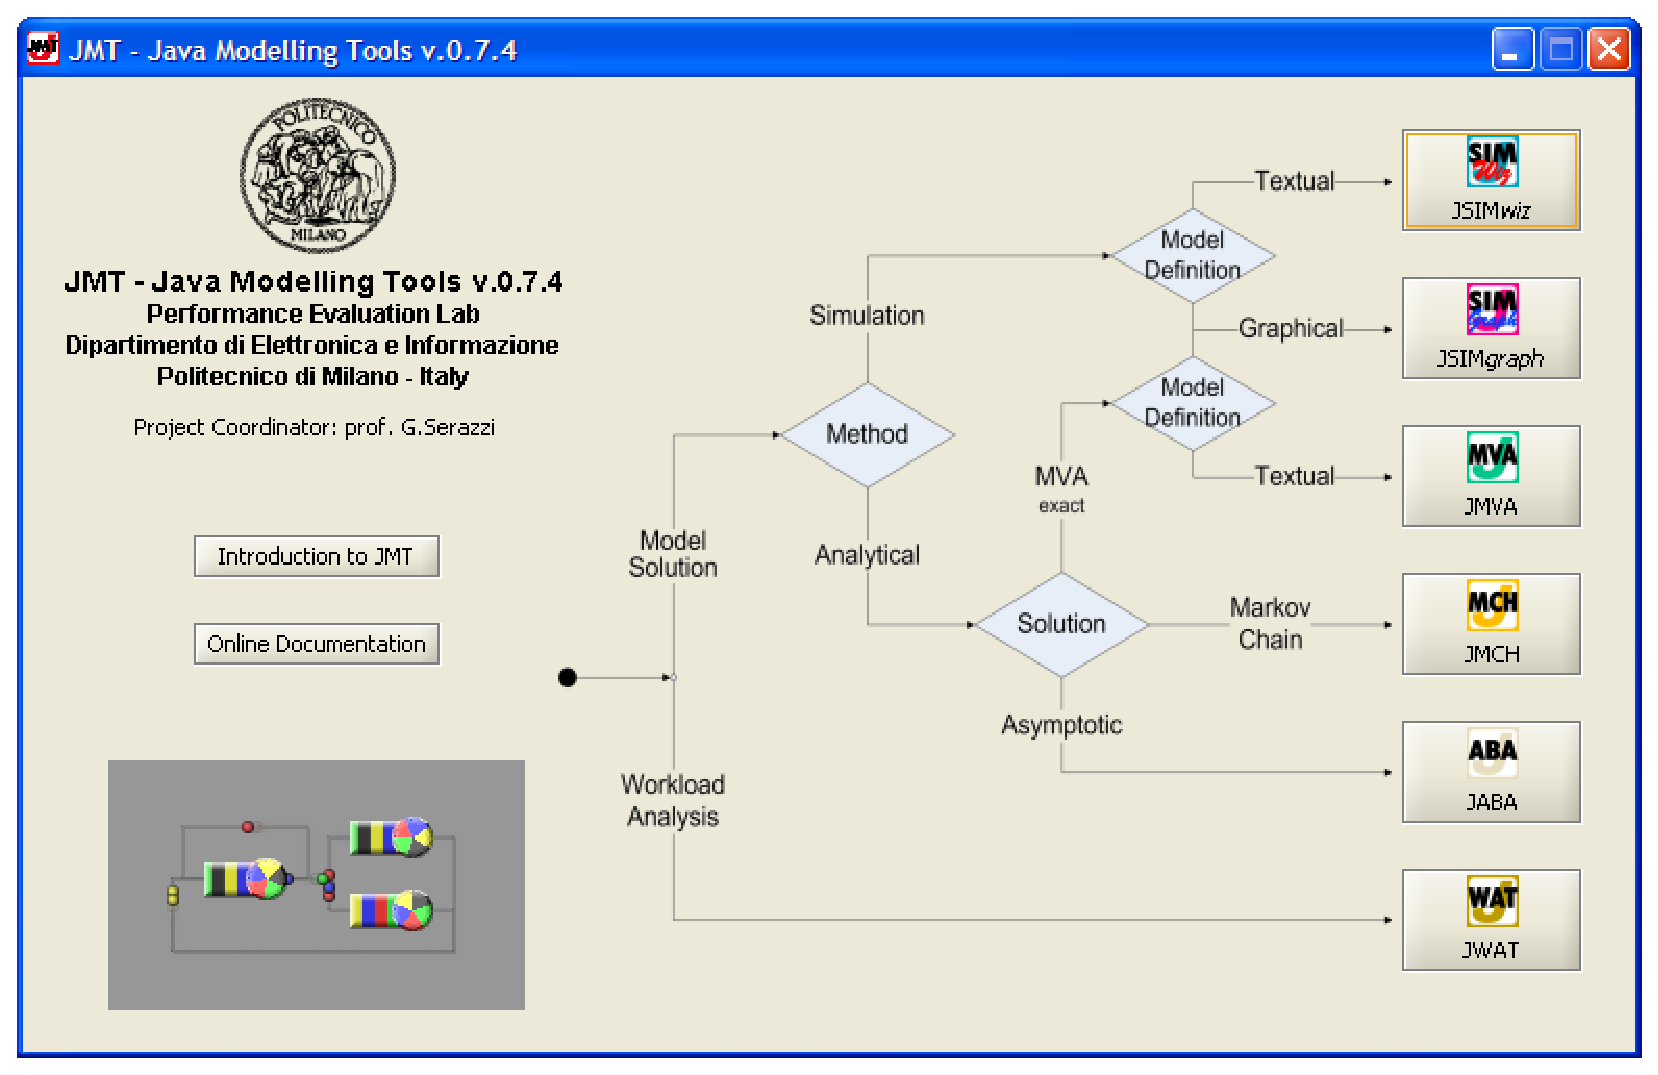
\includegraphics[scale=.5]{img/StartScreen}
    \end{center}
    \caption{The JMT suite Starting Screen}
    \label{fig:startscreen}
\end{figure}

This starting screen is used to select the application of the
suite to be executed by clicking on the corresponding button. The
flow chart should help the user to select the application that
best fits its needs.

In the following chapters the tools will be examined in details
and some examples are given. This manual is intended for the
general user that wants to learn how to interact with JMT.
Advanced users that want to learn details on internal data
structures, computational engines and XML interfaces should refer
to \emph{JMT system manual}.\\
Several other documents related to JMT description and
applications are provided with the suite. Click on \texttt{Online
Documentation} button to access the library. An exercise
book is also available.\\

%
% This document is free; you can redistribute it and/or modify
% it under the terms of the GNU General Public License as published by
% the Free Software Foundation; either version 2 of the License, or
% (at your option) any later version.
%
% This document is distributed in the hope that it will be useful, but
% WITHOUT ANY WARRANTY; without even the implied warranty of
% MERCHANTABILITY or FITNESS FOR A PARTICULAR PURPOSE.  See the GNU
% General Public License for more details.
%
% You should have received a copy of the GNU General Public License
% along with this document; if not, write to the Free Software
% Foundation, Inc., 51 Franklin Street, Fifth Floor, Boston, MA
% 02110-1301, USA.
%
% Author: Bertoli Marco
%
\chapter{JMVA}
\label{cha:jmva}
\section{Overview}
JMVA solves open, closed and mixed product form \cite{BCMP} queueing
networks with the exact MVA algorithm \cite{MVA}. In order to avoid
fluctuations of the solutions when the model contains load dependent
stations, the implemented algorithm is a stabilized version
\cite{AMVA} of the classic MVA algorithm.

Resources may be of two types: \emph{queueing} (either with
\texttt{load independent} or \texttt{load dependent} service times)
and \texttt{delay}. The model is described in alphanumeric way: user
is guided through the definition process by steps of a \emph{wizard}
interface (5 or 6 steps). What-if analyses, where a sequence of model are solved for different
values of parameters, are also possible (see \autoref{sec:jmva:whatif}). A graphical interface to describe the model in a user-friendly environment is also available, see \autoref{cha:jmodel} for details.

\subsection{Starting the alphanumeric MVA solver}
Selecting 
\includegraphics[scale=.5]{img/JMVAIcon} button on the
starting screen, \autoref{fig:jmva:Classes} window shows up.
\begin{figure}[htbp]
    \begin{center}
        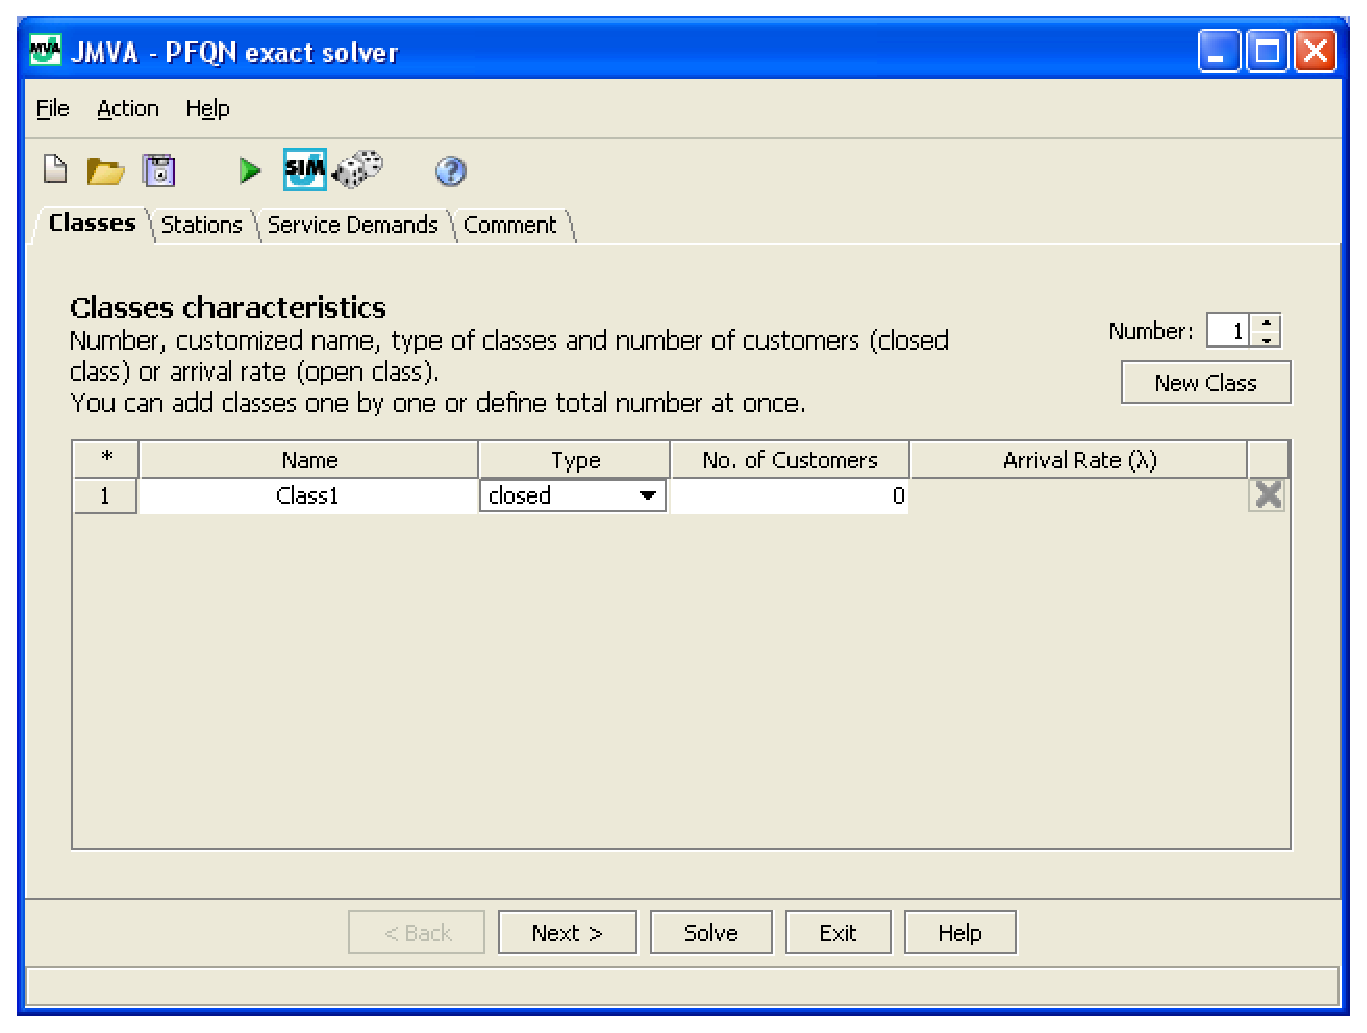
\includegraphics[scale=.5]{img/jmva/classes}
    \end{center}
    \caption{Classes tab}
    \label{fig:jmva:Classes}
\end{figure}
Three main areas are shown:
\begin{description}
\item[Menu :] it is organized into three groups of functions. To use a
menu, click on the menu heading and choose the appropriate option.
For the description of menu entries, see \autoref{sec:jmva:Menu}
\item[Toolbar :] contains some buttons to speed up access to JMVA functions
(e.g. New model, Open, Save\dots See \autoref{sec:jmva:Menu} for
details). If you move the mouse pointer over a button a tooltip will
be shown up.
\item[Page Area :] this is the core of the window. All MVA parameters are grouped in
different tabs. You can modify only a subset of them by selecting
the right tab, as will be shown later.
\end{description}

\section{Model definition}
Models with one or multiple customer classes provide estimates of
performance measures. For a brief description of basic terminology
please refer to \autoref{cha:glossary}.

In the case of single class models, the workload is characterized by
two inputs: the set of service demands, one for each resource, and
the workload intensity. On the other hand, in multiple class models,
a matrix of service demands is requested \cite{Lazowska}.

\subsection{Defining a new model}
To define a new model select toolbar button

\includegraphics[scale=.8]{img/jmva/new} or the \emph{New} command
from \emph{File} menu. The following parameters must be defined:
\begin{enumerate*}
\item \texttt{Classes} with their workload intensities (number of customer
$N$ for closed classes and arrival rate $\lambda$ for open classes)
\item \texttt{Stations} (service centers)
\item \texttt{Service demands} (or Service Times and Visits)
\item Optional short \texttt{Comment}
\end{enumerate*}

The execution of JMVA provides, for each class and each station, the
following performance indices:

\begin{itemize*}
\item Throughput
\item Queue Length
\item Residence Time
\item Utilization
\end{itemize*}

\noindent The following \emph{aggregate} indices are provided:
\begin{itemize*}
\item System Throughput
\item System Response Time
\item Average number of customers in the system
\end{itemize*}

\subsubsection{Input tabs}
As can be seen in \autoref{fig:jmva:Classes}, the parameters that
must be entered in order to define a new model are divided in four
tabs: \texttt{Classes}, \texttt{Stations}, \texttt{Service Demands}
and \texttt{Comment}.

Tabs number can become five, if you click  \emph{Service Times and
Visits} button in \texttt{Service Demands Tab}. As will be discussed
in \autoref{sec:jmva:ServiceDemand}, the \texttt{Service Demands
Tab} will be hidden and it will appear \texttt{Service Times Tab}
and \texttt{Visit Tab}. You can navigate through tabs:
\begin{itemize*}
\item using sequential wizard buttons, if enabled, at the bottom of
the window (\autoref{fig:jmva:Wizardbuttons})
\item using sequential buttons located in menu
\item using the tab selector, clicking on the corresponding
tab (\autoref{fig:jmva:Tabselector})
\end{itemize*}

\begin{figure}[htbp]
    \begin{center}
        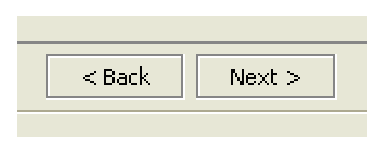
\includegraphics[scale=.5]{img/jmva/wizBut}
    \end{center}
    \caption{Wizard buttons}
    \label{fig:jmva:Wizardbuttons}
\end{figure}

\begin{figure}[htbp]
    \begin{center}
        
\includegraphics[scale=.5]{img/jmva/tabSel}
    \end{center}
    \caption{Tab selector}
    \label{fig:jmva:Tabselector}
\end{figure}

\subsection{Classes Tab}
An example screenshot of this tab can be seen in
\autoref{fig:jmva:Classes}. This tab allows to characterize customer
classes of the model. Your model will be a single class model if and
only if there will be only one class, closed or open. On the
contrary multiple class models will have at least two classes,
closed and/or open.

The number of classes in the model can be specified in the
corresponding input area, shown in \autoref{fig:jmva:ClassNum} and
can be modified using the keyboard or using the spin controls.

\begin{figure}[htbp]
    \begin{center}
        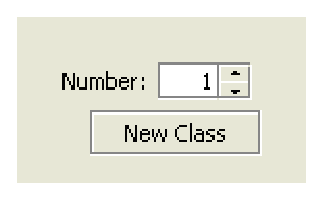
\includegraphics[scale=.5]{img/jmva/classNum}
    \end{center}
    \caption{Number of classes}
    \label{fig:jmva:ClassNum}
\end{figure}

Using the delete button

\includegraphics[scale=.6]{img/jmva/x} associated to a specific
class, a class can be removed provided that there will be at least
one class after the deletion. Similar result may be obtained using
spin controls, decreasing classes number; in this case last inserted
class will be removed.

Default class names are \emph{Class1}, \emph{Class2}, \dots
\emph{ClassN}. A model can be personalized by changing this names.

In \autoref{fig:jmva:3Classes} there are three classes of customers,
two closed and one open. The third class has the default name
\emph{Class3} while the other two classes have personalized names,
namely \emph{ClosedClass} and \emph{OpenClass}.

\begin{figure}[htbp]
    \begin{center}
        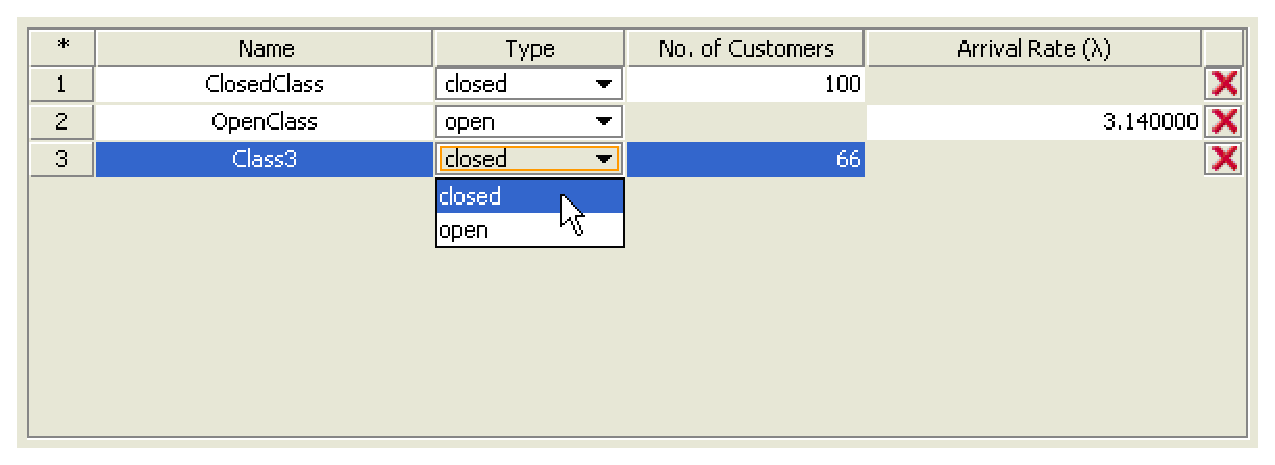
\includegraphics[scale=.5]{img/jmva/3classes}
    \end{center}
    \caption{Defining the classes types}
    \label{fig:jmva:3Classes}
\end{figure}

A class type can be \texttt{Open} or \texttt{Closed}. It is
important to define each class type because a closed class workload
is described by the number of customers in each class and the open
classes workload is described by the customer arrival rate for each
class.

As can be seen in \autoref{fig:jmva:3Classes}, a class type can be
selected in a combo-box. The input boxes \emph{No. of Customers
($N$)} referring to closed classes accept only positive integer
numbers; the input boxes of the \emph{Arrival Rate ($\lambda$)}
referring to open classes, accept positive real numbers
(\autoref{fig:jmva:workload}).

\begin{figure}[htbp]
    \begin{center}
        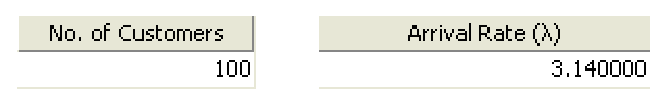
\includegraphics[scale=.5]{img/jmva/NL}
    \end{center}
    \caption{Workload definition of the number of customers of a closed
    class ($N=100$) and the arrival rate of an open class ($\lambda=3.14$)}
    \label{fig:jmva:workload}
\end{figure}

\subsection{Stations Tab}
The number of stations of the model can be specified in the
corresponding input area (\autoref{fig:jmva:stationNum}) and can be
modified using the keyboard or the spin controls.

\begin{figure}[htbp]
    \begin{center}
        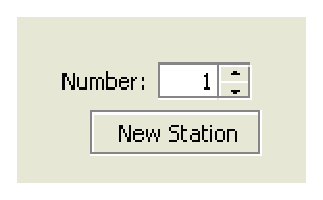
\includegraphics[scale=.5]{img/jmva/stationNum}
    \end{center}
    \caption{Number of stations}
    \label{fig:jmva:stationNum}
\end{figure}

Using the delete button

\includegraphics[scale=.6]{img/jmva/x} associated to a specific
station, a station can be removed provided that there will be at
least one station after the deletion. Similar result may be obtained
using spin controls, decreasing stations number; in this case last
inserted station will be removed.

Default station names are \emph{Station1}, \emph{Station2}, \dots
\emph{StationN}. In order to personalize your model, you can change
and give names other than default ones.

In \autoref{fig:jmva:stations} there is only one station with
default name \emph{Station4} and there are three stations with
personalized names: \emph{CPU}, \emph{Disk1} and \emph{Disk2}.

\begin{figure}[htbp]
    \begin{center}
        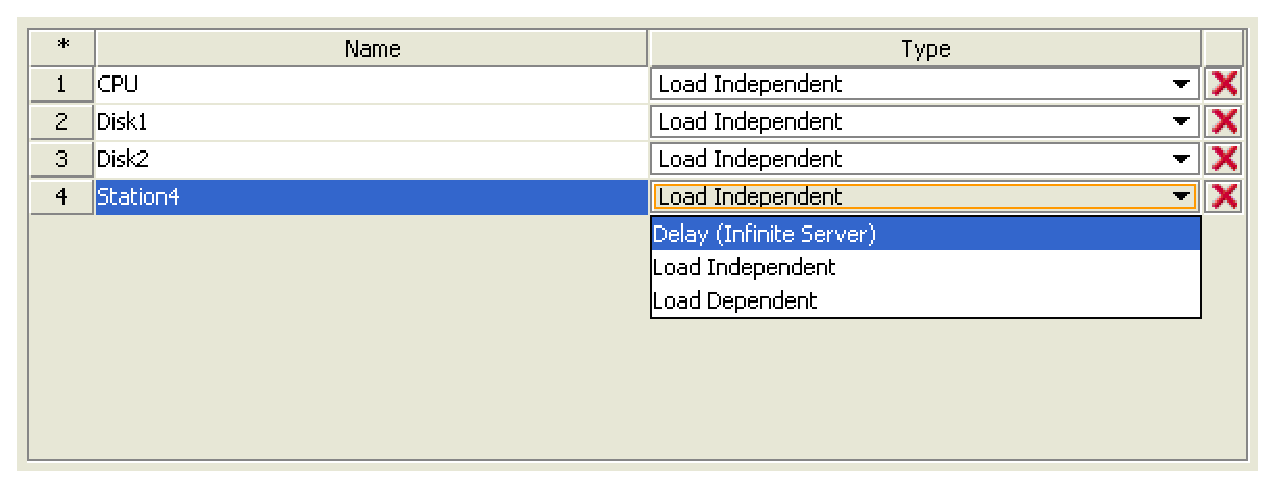
\includegraphics[scale=.5]{img/jmva/4stations}
    \end{center}
    \caption{Defining the stations type}
    \label{fig:jmva:stations}
\end{figure}

A station type can be \texttt{Load Independent}, \texttt{Load
Dependent} or \texttt{Delay}. You can insert in your model a
\texttt{Load Depend} center only if there is a unique closed
class\footnote{Multiclass, open and mixed models with load dependent
stations are not supported yet}; in all other cases the combo-box
will be disabled.

It is important to define each station type because if a station is
\texttt{Load Dependent} a set of service demand - or a set of
service times and the number of visit - must be defined (one service
demand/time for each possible value of queue length inside the
station).

In \autoref{sec:jmva:ServiceDemand} we will explain this concept
with more details.

\subsection{Service Demands, Service Times and Visits Tabs}
\label{sec:jmva:ServiceDemand} Service Demands can be defined in two
ways:
\begin{itemize*}
\item directly, by entering Service Demands ($D_{kc}$)
\item indirectly, by entering Service Times ($S_{kc}$) and Visits ($V_{kc}$)
\end{itemize*}

Service demand $D_{kc}$ is the total service requirement, that is
the average amount of time that a customer of class $c$ spends in
service at station $k$ during one interaction with the system, i.e.
it's complete execution. Service time $S_{kc}$ is the average time
spent by a customer of class $c$ at station $k$ for a single visit
at that station while $V_{kc}$ is the average number of visits at
that resource for each interaction with the system.

Remember that $D_{kc} = V_{kc} * S_{kc}$ so it's simple to compute
service demands matrix starting from service times and visits
matrixes. Inverse calculation is performed with the following
algorithm:
\[
V_{kj} = \left\{
\begin{array}{ccl} 1 & \textrm{if} & D_{kc} > 0 \\
0 & \textrm{if} & D_{kc} = 0 \end{array}\right.
\]
\[
S_{kc} = \left\{ \begin{array}{ccl} D_{kc} & \textrm{if} & D_{kc}
> 0 \\ 0 & \textrm{if} & D_{kc} = 0 \end{array}\right.
\]

\subsubsection{Service Demands Tab}
In this tab you can insert directly Service Demands $D_{kc}$ for
each pair \{station~$k$-class~$c$\} in the model. In
\autoref{fig:jmva:ServiceDemandsTab} a reference screenshot can be
seen: notice that a value for every $D_{kc}$ element of the
$D$-matrix has already been specified because default value assigned
to newly created stations is zero.

\begin{figure}[htbp]
    \begin{center}
        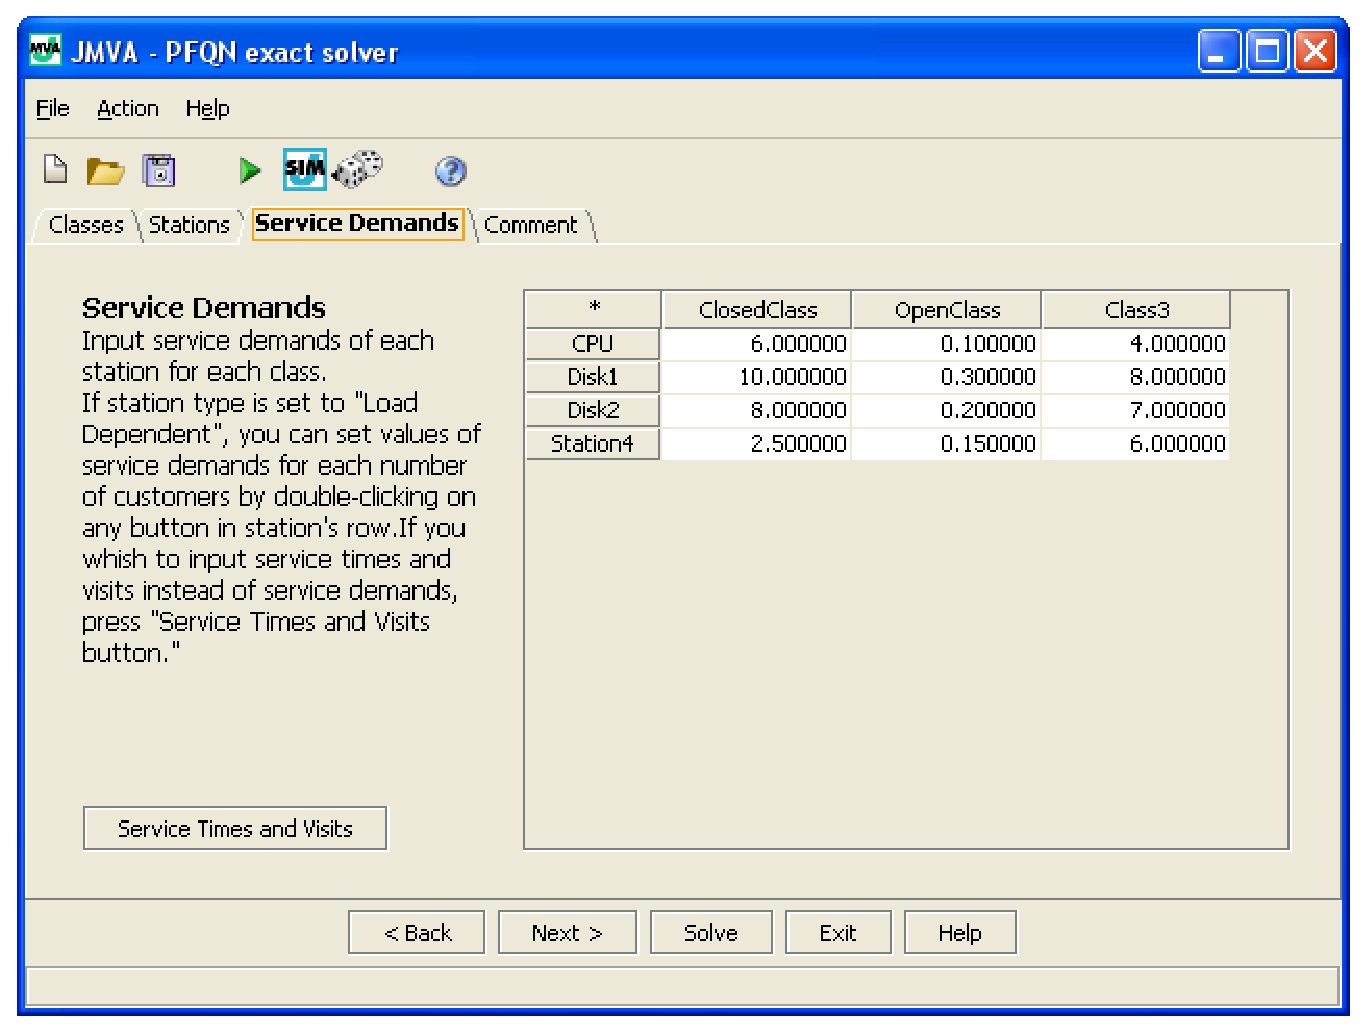
\includegraphics[scale=.5]{img/jmva/serviceDemands}
    \end{center}
    \caption{The Service Demands Tab}
    \label{fig:jmva:ServiceDemandsTab}
\end{figure}

In the example of \autoref{fig:jmva:ServiceDemandsTab}, each job of
type \emph{ClosedClass} requires an average service demand time of 6
sec to \emph{CPU}, 10 sec to \emph{Disk1}, 8 sec to
\emph{Disk2} and 2.5 sec to \emph{Station4}.\\
On the other hand, a job of type \emph{OpenClass} requires on
average 0.1 sec of \emph{CPU} time, 0.3 sec of \emph{Disk1} time,
0.2 sec of \emph{Disk2} time and 0.15 sec of \emph{Station4} time to
be processed by the system.

If the model contains any load dependent station, the behavior of
\autoref{fig:jmva:LD} will be shown.

\begin{figure}[htbp]
    \begin{center}
        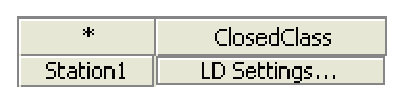
\includegraphics[scale=.5]{img/jmva/ld}
    \end{center}
    \caption{Defining a \emph{load dependent} station service demand}
    \label{fig:jmva:LD}
\end{figure}

By double-clicking on \emph{LD Settings\dots} button a window will
show up and that can be used to insert the values of the service
demands for each possible number of customer inside the station.
That values can be computed by evaluating an analytic function as
shown in \autoref{fig:jmva:LDEdit}. The list of supported operators
and more details are reported in \autoref{sec:jmva:JEP}.

\begin{figure}[htbp]
    \begin{center}
        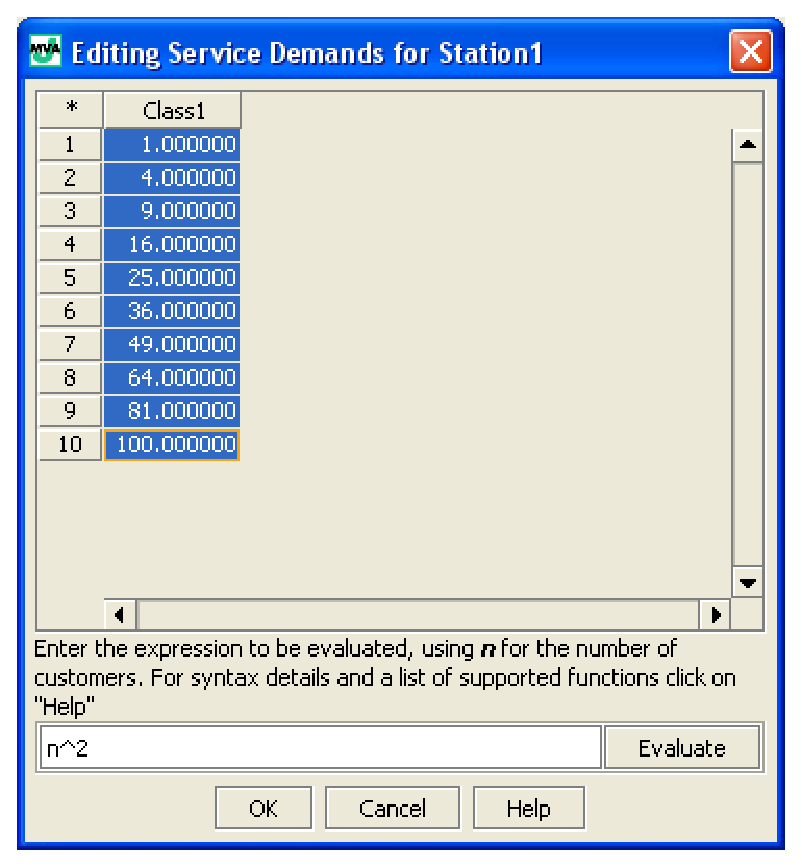
\includegraphics[scale=.5]{img/jmva/ldEdit}
    \end{center}
    \caption{Load Dependent editing window}
    \label{fig:jmva:LDEdit}
\end{figure}

\subsubsection{Service Times and Visits Tabs}
In the former tab you can insert the Service Times $S_{kc}$ for each
pair \{station~$k$-class~$c$\} in the model, in the latter you can
enter the visits number $V_{kc}$ (See \autoref{fig:jmva:visits}).

\begin{figure}[htbp]
    \begin{center}
        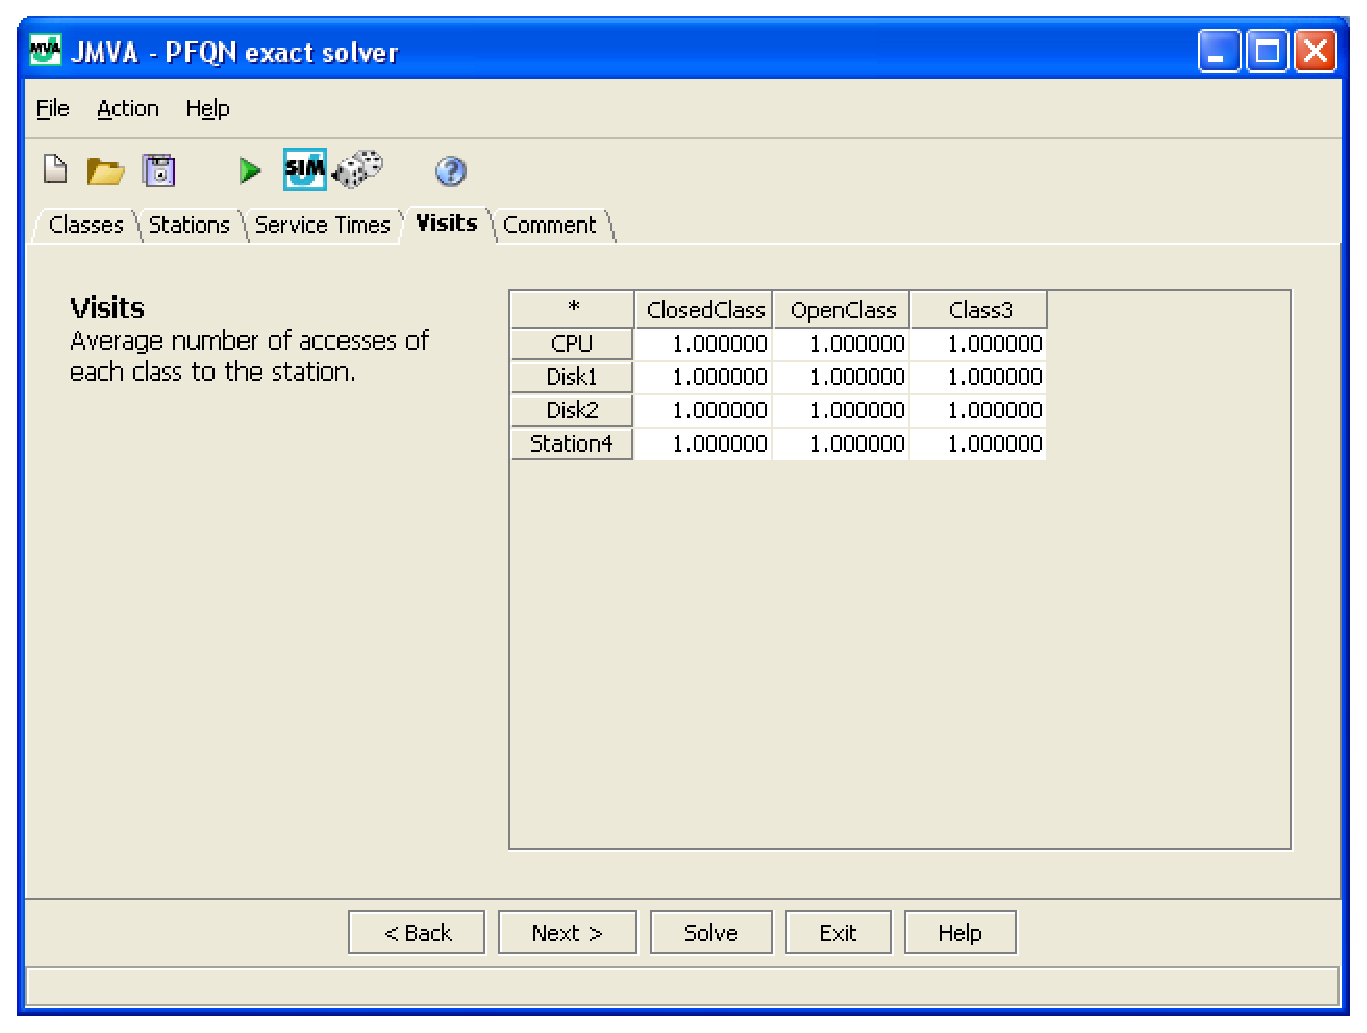
\includegraphics[scale=.5]{img/jmva/visits}
    \end{center}
    \caption{Visits Tab}
    \label{fig:jmva:visits}
\end{figure}

The layout of these tabs is similar to the one of the
\texttt{Service Demand Tab} described in the previous paragraph. The
default value for each element of the Service Times ($S$) matrix is
zero, while it's one for Visits' matrix elements.

In current model contains load dependent stations, the behavior of
\texttt{Service Times Tab} for their parametrization will be
identical to the one described on the previous paragraph for
\texttt{Service Demands Tab}. On the other hand \texttt{Visits Tab}
behavior won't change as load dependency is a property of service
times and not of visits.

\subsection{What-if Tab}
\label{sec:jmva:whatif} This Tab is used to perform a what-if
analysis, i.e. solve multiple models changing the value of a
\texttt{control parameter}. In \autoref{fig:jmva:whatifDisabled} is
shown this panel when what-if analysis is disabled.

\begin{figure}[htbp]
    \begin{center}
        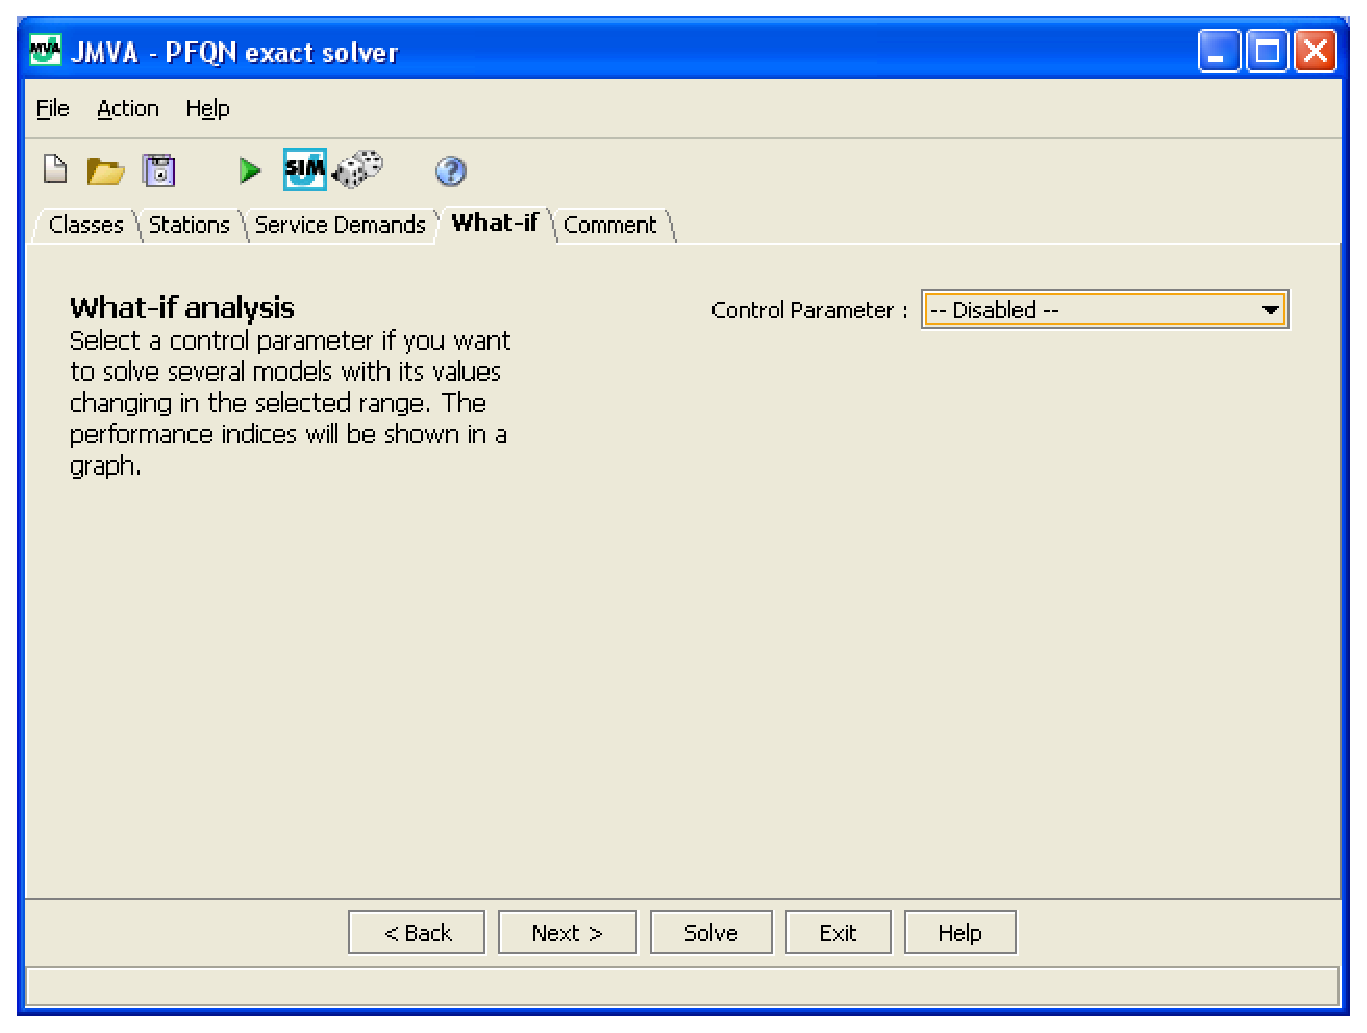
\includegraphics[scale=.5]{img/jmva/whatifDisabled}
    \end{center}
    \caption{What-if Tab - Disabled analysis}
    \label{fig:jmva:whatifDisabled}
\end{figure}

The first parameter to be set is the \texttt{control parameter} i.e.
the parameter that will be changed to solve different models in a
selected range. Five choices are possible:
\begin{description*}
\item[Disabled :] disables what-if analysis, so only a single queueing network
model, specified in the previous steps, will be solved. This is the
\emph{default} option.
\item[Customer Numbers :] different models will be
executed by changing the \texttt{number of customers} of a single
\texttt{closed} class or of every closed class proportionally. This
option is available only when current model has at least one closed
class.
\item[Arrival Rates :] different models will be
executed by changing \texttt{arrival rate} of a single \texttt{open}
class or of every open class proportionally. This option is
available only when current model has at least one open class.
\item[Population Mix :] the total number of customers will be kept
constant, but the population mix (i.e. the ratio between
\texttt{number of customers} of selected closed class $i$ and the
total number of customers in the system $\beta_i = N_i / \sum_k
N_k$). This option is available only when current model has two
closed classes.
\item[Service Demands :] different models will be solved changing
the \texttt{service demand} value of a given station for a given
class or for all classes proportionally. This option is available
only for \texttt{load independent} and \texttt{delay} stations.
\end{description*}

Whenever a control parameter is selected, the window layout will be
changed to allow the selection of a valid range of values for it.
For example in \autoref{fig:jmva:whatifDemands} \texttt{Service
Demands} control parameter was selected. On the bottom of the
window, a riepilogative table is presented: depending on selected
control parameter, that table is used to show the \emph{initial
state} of involved parameters. Every class currently selected for
what-if analysis is shown in red.

\begin{figure}[htbp]
    \begin{center}
        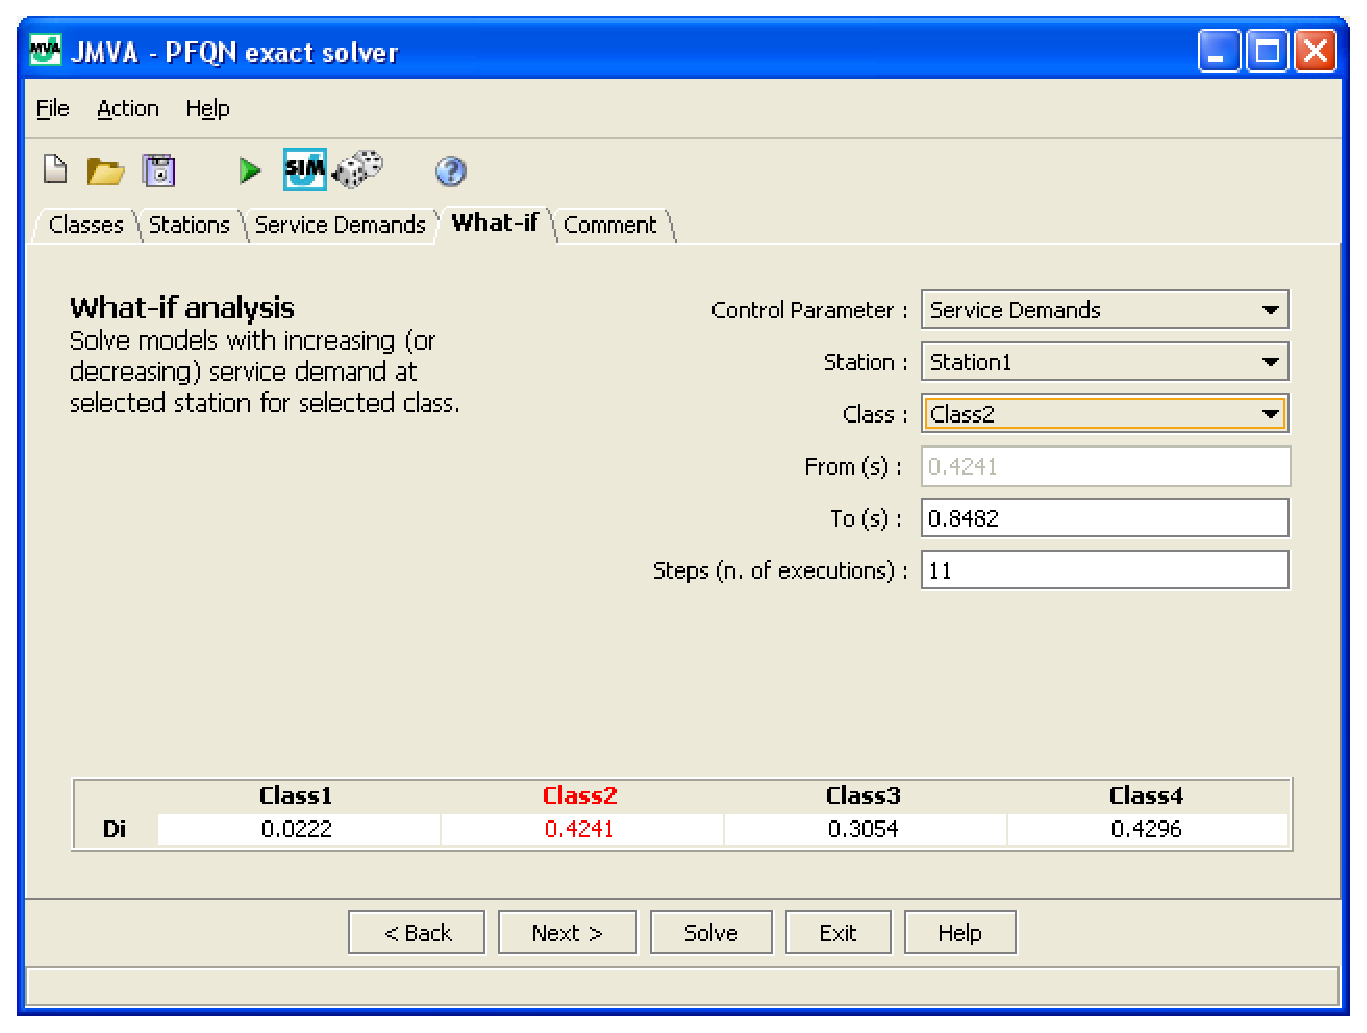
\includegraphics[scale=.5]{img/jmva/whatifDemands}
    \end{center}
    \caption{What-if Tab - Service Demands}
    \label{fig:jmva:whatifDemands}
\end{figure}

A brief description of each field is now presented:
\begin{description*}
\item[Station :] available only with \texttt{Service Demands} control
parameter. This combo box allows to select at which station service
demand values will be modified.
\item[Class :] allow to select for which class the selected
parameter will be changed. A special value, namely \texttt{All
classes proportionally}, is used to modify the control parameter for
each class keeping constant the proportion between different
classes\footnote{for example, in a model with two closed classes
with population vector (2,6), the following models can be executed:
(1,3), (2,6), (3,9), (4, 12), \dots}. This special value is not
available in \texttt{Population Mix} analysis as we are changing the
proportion of jobs between two closed classes.
\item[From :] the initial value of what-if analysis. It was chosen
to leave this value fixed to the initial value specified by the user
in the previous steps to avoid confusions, so this field acts as a
reminder. The only exception is when \texttt{Population Mix} is
changed, in that case it's allowed to modify this value too.
\item[To :] the final value of what-if analysis. Please notice that
this value can be greater or smaller than \texttt{From} value and is
expressed in the same measure unit. Whenever \texttt{All classes
proportionally} option is selected, both \texttt{From} and
\texttt{To} values are expressed as percentages of initial values
(specified in the previous steps and reminded in the table at the
bottom of the panel, see \autoref{fig:jmva:whatifDemands}), in the
other situations they are considered as absolute values for the
chosen parameter.
\item[Steps :] this is chosen number of executions i.e. the number
of different models that will be solved. When control parameter is
\texttt{Customer Numbers} or \texttt{Population Mix}, the model can
be correctly specified only for integer values of population. JMVA
will perform a fast computation to find the maximum allowed number
of executions given current \texttt{From} and \texttt{To} values: if
user specify a value bigger than that, JMVA will use the computed
value.
\end{description*}


\subsection{Comment Tab}
In this Tab, a short - optional - comment about the model can be
inserted; it will be saved with the other model parameters.

\subsection{Expression Evaluator}
\label{sec:jmva:JEP} An expression evaluator is used for the
definition of service demands or service times of a load dependent
station. It allows to specify times as an analytic function of $n$
where $n$ is the number of customer inside the station.

Expression are evaluated using
\emph{JEPLite}\footnote{http://jeplite.sourceforge.net/} (Java Math
Expression Parser enlited) package which supports all operators
enumerated in \autoref{tab:jmva:Operators} and all functions
enumerated in \autoref{tab:jmva:Functions}.

\begin{table}[htbp]
\begin{center}
\begin{tabular}{|c|c|}
Operator & Symbol\\
\hline
Power & $^{\wedge}$\\
Unary Plus, Unary Minus & $+n$, $-n$\\
Modulus & $\%$\\
Division & $/$ \\
Multiplication & $*$\\
Addition, Subtraction & $+$, $-$\\
\hline
\end{tabular}
\end{center}
\caption{List of all supported operators ordered by priority}
\label{tab:jmva:Operators}
\end{table}

\begin{table}[htbp]
\begin{center}
\begin{tabular}{|c|c|}
Function & Symbol\\
\hline
Sine & sin()\\
Cosine & cos()\\
Tangent & tan()\\
Arc Sine & asin()\\
Arc Cosine & acos()\\
Arc Tangent & atan()\\
Hyperbolic Sine & sinh()\\
Hyperbolic Cosine & cosh()\\
Hyperbolic Tangent & tanh()\\
Inverse Hyperbolic Sine & asinh()\\
Inverse Hyperbolic Cosine & acosh()\\
Inverse Hyperbolic Tangent & atanh()\\
Natural Logarithm & ln()\\
Logarithm base 10 & log()\\
Absolute Value / Magnitude & abs()\\
Random number $[0,1]$ & rand()\\
Square Root & sqrt()\\
Sum & sum()\\
\hline
\end{tabular}
\end{center}
\caption{List of supported functions for the load dependent service
times} \label{tab:jmva:Functions}
\end{table}

\subsection{Model Solution}
\label{sec:jmva:solution}Use \texttt{Solve} command to solve the
model. If the model specify a what-if analysis, please refer to
\autoref{sec:jmva:solutionWhatif}. Model results will be shown on a
separate window, like the one of \autoref{fig:jmva:results}.

\begin{figure}[htbp]
    \begin{center}
        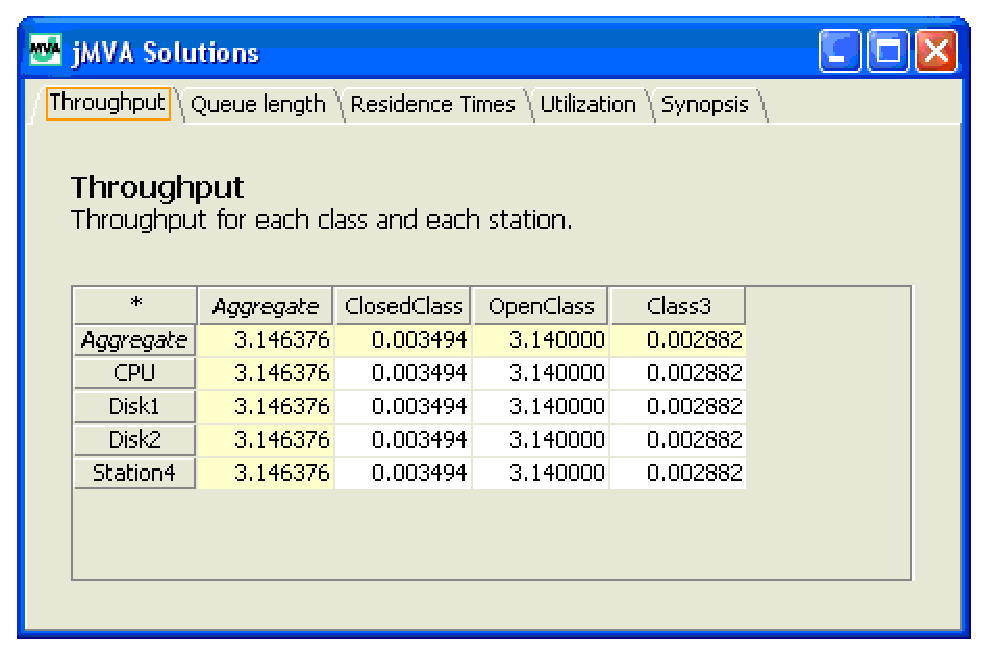
\includegraphics[scale=.5]{img/jmva/results}
    \end{center}
    \caption{Model Solution (Throughput Tab)}
    \label{fig:jmva:results}
\end{figure}

Using the tab selector, all the other computed performance indices
can be seen: Throughput, Queue lengths, Residence Times,
Utilizations and a synopsis panel with schematic report of input
model. Both results and synopsis tab data can be copied to clipboard
with \texttt{CTRL+C} keyboard shortcut.

When open classes are used, the resource saturation control is
performed. For multiple class models, the following inequality must
be satisfied:
\[
{\max_k {\sum_c{\lambda_c * D_{kc}}}} < 1
\]
This inequality ensures that no service center is saturated as a
result of the combined loads of all the classes. Let us consider, as
example, the model with the classes shown in
\autoref{fig:jmva:3Classes} with the D-matrix shown in
\autoref{fig:jmva:ServiceDemandsTab} Since $\lambda = 3.14 < 3.33 =
1 / 0.3 = 1 / D_{max}$ the model is not in saturation and the
\texttt{Solve} command will be executed correctly.

In this example, substituting $D_{\textrm{Disk1-OpenClass}}$ with
values $\geq 1/3.14 \approx 0.318$ will cause the saturation of
resource \emph{Disk1} and the error message of
\autoref{fig:jmva:saturation} will appear.

\begin{figure}[htbp]
    \begin{center}
        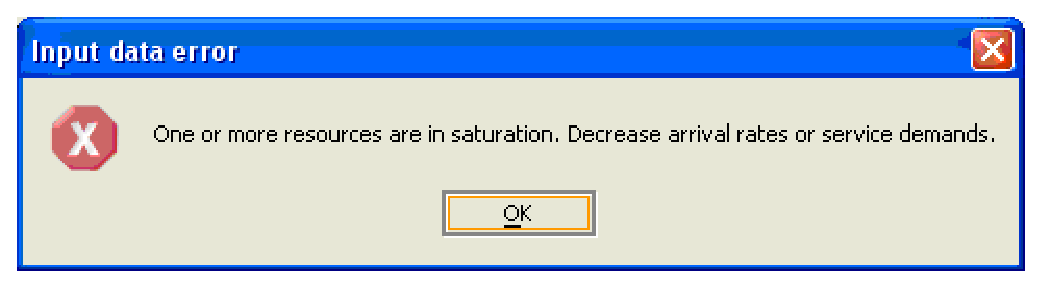
\includegraphics[scale=.5]{img/jmva/saturation}
    \end{center}
    \caption{Input data error message }
    \label{fig:jmva:saturation}
\end{figure}

\subsection{Model Solution - What-if analysis}
\label{sec:jmva:solutionWhatif}Use \texttt{Solve} command to solve
the model. During model solution, a progress window, see
\autoref{fig:jmva:progress}, shows up. It displays the cumulative
number of models currently solved, the total number of models to be
solved and the elapsed time.

\begin{figure}[htbp]
    \begin{center}
        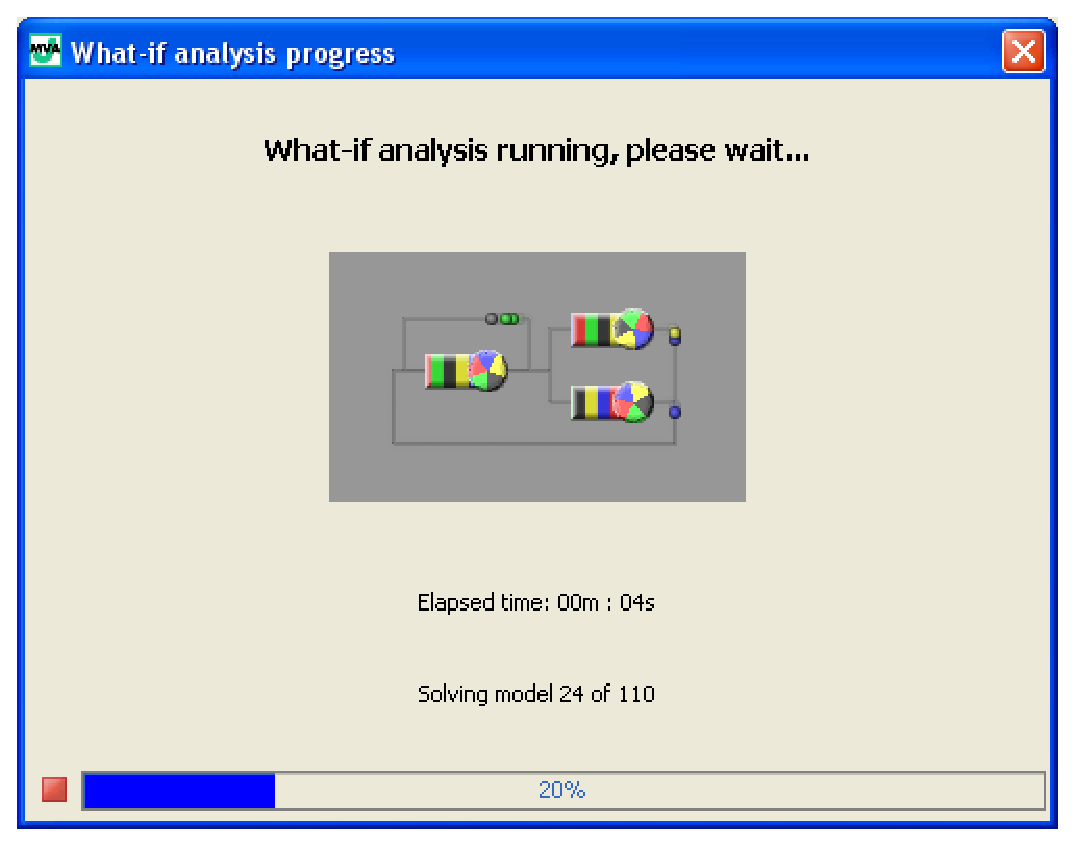
\includegraphics[scale=.5]{img/jmva/progress}
    \end{center}
    \caption{Model Solution progress window}
    \label{fig:jmva:progress}
\end{figure}

At the end of the solution, results will be shown in a separate
window, see \autoref{fig:jmva:graphical}.
\begin{figure}[htbp]
    \begin{center}
        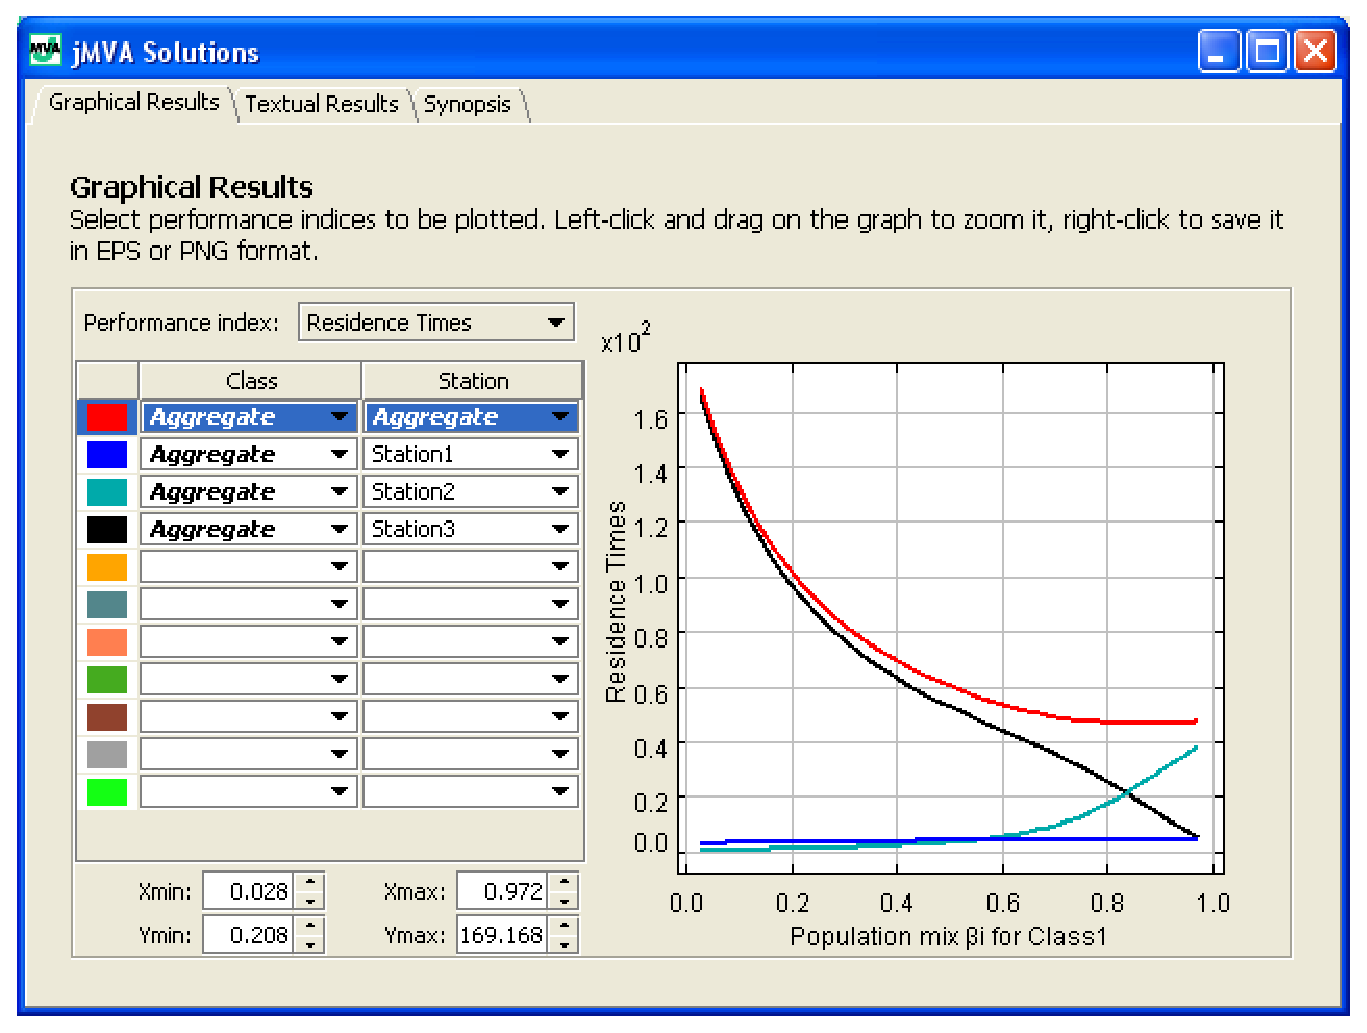
\includegraphics[scale=.5]{img/jmva/Graphical}
    \end{center}
    \caption{Model Solution - Graphical Results Tab}
    \label{fig:jmva:graphical}
\end{figure}
This tab allows to show in a plot the relation between the chosen
control parameter (see \autoref{sec:jmva:whatif}) and the
performance indices computed by the analytic engine.

The combo box \texttt{Performance Index} allows to select the
performance index to be plotted in the graph, while in the table
below, users can select the resource and the class considered.
\begin{itemize*}
\item The first column is fixed and lists all available colors to be
used in the graph.
\item The second column, named \texttt{Class}, is used to select the
class considered in the graph. The special value \texttt{Aggregate}
is used for the aggregate measure for all classes. If input model is
single-class, the class is selected by default for each row.
\item The final column, named \texttt{Station}, is used to select the
station considered in the graph. The special value
\texttt{Aggregate} is used for the aggregate measure for the entire
network. Note that the \texttt{Aggregate} value is not valid when
the \texttt{Utilization} performance index is selected.
\end{itemize*}

In addition to the \emph{center} performance indices (i.e.
\texttt{Throughput}, \texttt{Queue length}, \texttt{Residence
Times}, \texttt{Utilization}), three \emph{system} performance
indices are provided  in the \texttt{Performance Index} combo box
(\texttt{System Response Time}, \texttt{System Throughput},
\texttt{Number of Customers}). This \emph{system} indices can be
easily obtained by selecting the special \texttt{Aggregate} value
for both \texttt{Class} and \texttt{Station} columns of the
corresponding center indices (see \autoref{cha:glossary} for the
definition of the performance indices), but they were provided here
as a \emph{shortcut}. As we are referring to aggregate measures, the
selection of reference class and station is not significant and, in
this case, the table in the left of \autoref{fig:jmva:graphical}
will not be shown.

On the bottom-left corner of the window, users can modify minimum
and maximum value of both X and Y axis of the plot. JMVA is designed
to automatically best-fit the plot in the window but this controls
allow the user to specify a custom range or zoom on the plot.
Another fast method to perform a zoom operation is to left-click and
drag a rectangle on the graphic window (see
\autoref{fig:jmva:zoomDrag}) or right-click on it and select
\texttt{Zoom in} or \texttt{Zoom out} options. To automatically
reset the best-fit scale users can right-click on the graphic window
and select \texttt{Original view} option.

\begin{figure}[htbp]
    \begin{center}
        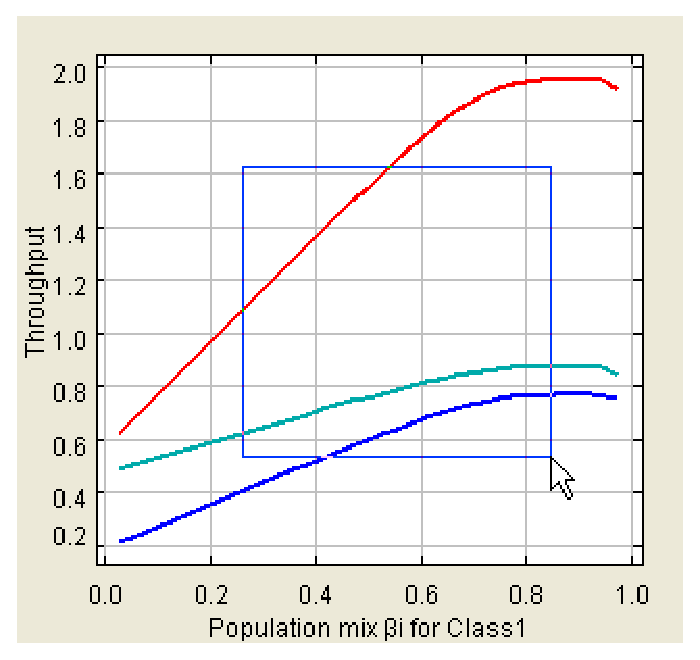
\includegraphics[scale=.5]{img/jmva/whatIfDrag}
    \end{center}
    \caption{Zoom operation on the plot}
    \label{fig:jmva:zoomDrag}
\end{figure}

The graphic window allows to export plots as image to be included in
documents and presentations. To save current graph as image,
right-click on the graphic and select \texttt{Save as\dots} option.
A dialog will be shown to request the name of the file and the
format. Currently supported format are Portable Network Graphics -
PNG - (raster) and Encapsulated PostScript - EPS - (vectorial,
currently only black and white).

The second tab of the solution window, shown in
\autoref{fig:jmva:textualResults}, is used to display the solutions
of each execution of the analytic algorithm.

\begin{figure}[htbp]
    \begin{center}
        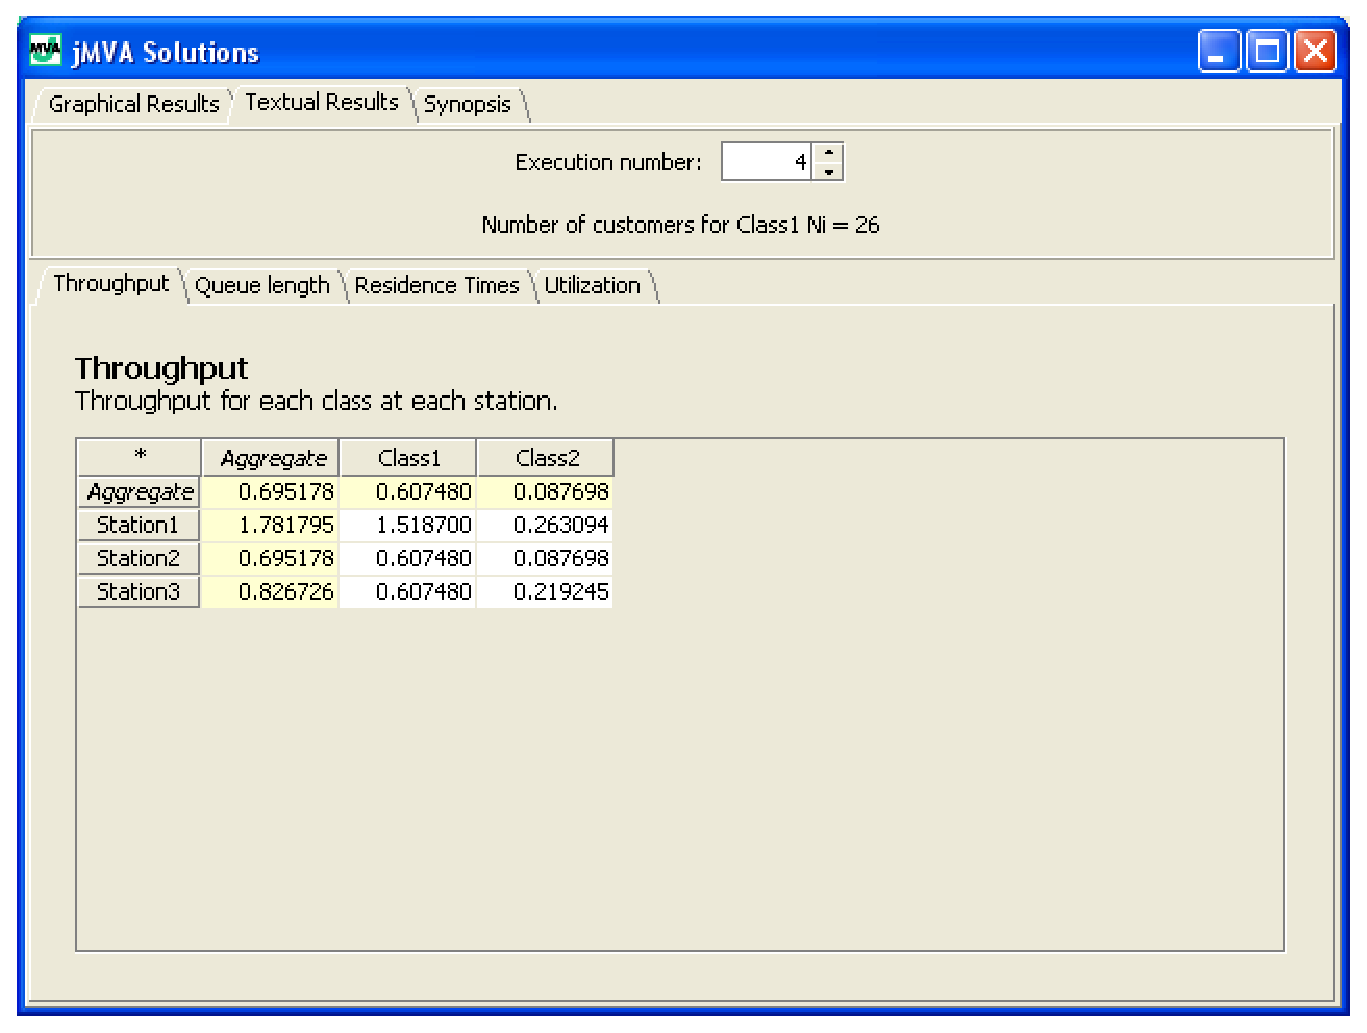
\includegraphics[scale=.5]{img/jmva/textualResults}
    \end{center}
    \caption{Model Solution - Textual Results Tab}
    \label{fig:jmva:textualResults}
\end{figure}

This Tab has the same structure of the results window without
What-if analysis (described in \autoref{sec:jmva:solution}) but
allows to select the execution to be shown in the field
\texttt{Execution Number}. By entering requested execution number in
the spinner, or using the \emph{up} and \emph{down} arrows, user can
cycle between all the computed performance indices for each
execution. Just below the spinner, a label gives information on the
value of the control parameter for the currently selected execution.

\subsection{Modification of a model}
To modify system parameters return to the main window and enter new
data. After the modifications, if you use \texttt{Solve} command, a
new window with model result will show. You can \texttt{save} this
new model with the previous name - overwriting the previous one - or
\texttt{save} it with a different name or in a different directory.

\section{Menu entries}
\label{sec:jmva:Menu}
\subsection{File}
\subsubsection{New}
Use this command in order to create a new JMVA model.

\noindent
\begin{tabular}{ll}
Shortcut on Toolbar: & 
\includegraphics[scale=.8]{img/jmva/new}\\
Accelerator Key: & CTRL+N
\end{tabular}

\subsubsection{Open}
Use this command to open an existing model. You can only open one
model at time, to edit two or more models start more than one
instance of JMVA. If current model was modified since its creation
or last save action, a popup window will be shown for confirmation.

It's possible to open not only models saved with JMVA (*.jmva), but
also with other programs of the suite (for example JABA *.jaba, JSIM
*.jsim and JMODEL *.jmodel). Whenever a foreign data file is opened, a
conversion is performed and error/warnings occurred during
conversion will be reported in a window.

Models are stored in XML format, see \emph{JMT system manual} for a
detailed description.

\noindent
\begin{tabular}{ll}
Shortcut on Toolbar: & 
\includegraphics[scale=.8]{img/jmva/open}\\
Accelerator Key: & CTRL+O
\end{tabular}

\subsubsection{Save}
Use this command in order to save the active document with its
current name in the selected directory.

When you save a document for the first time, JMVA displays the Save
As dialog box so you can rename your document. If you save a model
after its resolution, results are stored with model definition data.

\noindent
\begin{tabular}{ll}
Shortcut on Toolbar: & 
\includegraphics[scale=.8]{img/jmva/save}\\
Accelerator Key: & CTRL+S
\end{tabular}

\subsubsection{Exit}
Use this command in order to end a JMVA session. You can also use
the Close command on the application Control menu. If current model
was modified since its creation or last save action, a popup window
will be shown for confirmation.

\noindent
\begin{tabular}{ll}
\\
Accelerator Key: & CTRL+Q
\end{tabular}

\subsection{Action}
\subsubsection{Solve}
Use this command when model description is terminated and you want
to start the solution of the model. At the end of the process the
window in \autoref{fig:jmva:results} will popup.

\noindent
\begin{tabular}{ll}
Shortcut on Toolbar: & 
\includegraphics[scale=.8]{img/jmva/solve}\\
Accelerator Key: & CTRL+L
\end{tabular}

\subsubsection{Randomize}
Use this command in order to insert random values into Service
Demands - or Service Times - table. Generated values are
automatically adjusted to avoid saturation of resources.

\noindent
\begin{tabular}{ll}
Shortcut on Toolbar: & 
\includegraphics[scale=.8]{img/jmva/randomize}\\
Accelerator Key: & CTRL+R
\end{tabular}

\subsubsection{Import in JSIM}
This command will import current model into JSIM to solve it using
simulator. A simple parallel topology is derived from number of
visits at each station and generated model is equivalent to original
one.

\noindent
\begin{tabular}{ll}
Shortcut on Toolbar: & 
\includegraphics[scale=.8]{img/jmva/toJSIM}\\
Accelerator Key: & CTRL+G
\end{tabular}

\subsection{Help}
\subsubsection{JMVA Help}
Use this command to display application help. From the initial
window, you can jump to step-by-step instructions that show how use
JMVA and consult various types of reference information.

Once you open Help, you can click the Content button whenever you
want to return to initial help window.

\noindent
\begin{tabular}{ll}
Shortcut on Toolbar: & 
\includegraphics[scale=.8]{img/jmva/help}\\
Accelerator Key: & CTRL+Q
\end{tabular}

\subsubsection{About}
Use it in order to display information about JMVA version and
credits.

\section{Examples}
In this section we will describe some examples of model
parametrization and solution using MVA exact solver. Step-by-step
instructions are provided in five examples:
\begin{enumerate*}
\item A single class closed model with three load independent stations and a delay service
center (\autoref{sec:jmva:example1})
\item A multiclass open model with two classes and three load independent
stations (\autoref{sec:jmva:example2})
\item A single class closed model with a load dependent station and
a delay (\autoref{sec:jmva:example3})
\item A multiclass mixed model with three stations (\autoref{sec:jmva:example4})
\item A multiclass closed model where a what-if analysis is used to find optimal
Population Mix values (\autoref{sec:jmva:example5})
\end{enumerate*}


\subsection{Example 1 - A model with a single closed class}
\label{sec:jmva:example1} Solve the single class model specified in
\autoref{fig:jmva:Example1topology}.
\begin{figure}[htbp]
    \begin{center}
        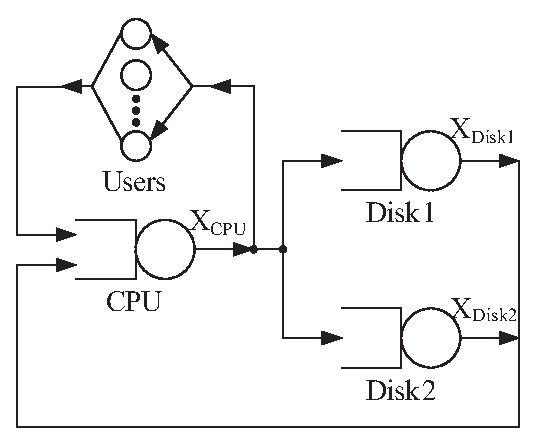
\includegraphics[scale=.65]{img/jmva/example1}
    \end{center}
    \caption{Example 1 - network topology}
    \label{fig:jmva:Example1topology}
\end{figure}
The customer class, named \emph{ClosedClass} has a population of $N
= 3$ customers.

There are four stations, three are of load independent type (named
\emph{CPU}, \emph{Disk1} and \emph{Disk2}) and one is of delay type
(named \emph{Users}). \emph{Users} delay station represents user's
\emph{think time} ($Z = 16$ s) between interaction with the system.
Service times and visits for stations are reported in
\autoref{tab:jmva:example1ServTimes}.

\begin{table}[htbp]
\begin{center}
\begin{tabular}{c|r|r|r|r|}
& \multicolumn{1}{c|}{CPU} & \multicolumn{1}{c|}{Disk1} & \multicolumn{1}{c|}{Disk2} & \multicolumn{1}{c|}{Users}\\
\hline
Service Times [s] & $0.006$ & $0.038$ & $0.030$ & $16.000$\\
Visits & $101.000$ & $60.000$ & $40.000$ & $1.000$\\
\hline
\end{tabular}
\end{center}
\caption{Example 1 - service times and visits}
\label{tab:jmva:example1ServTimes}
\end{table}

\subsubsection{Step 1 - Classes Tab}
\begin{itemize*}
\item use New command to create a new jMVA document
\item by default, you have already a \texttt{Closed} class
\item if you like, substitute default \emph{Class1} name with a customized
one (\emph{ClosedClass} in our example)
\item complete the table with workload intensity (number of customers). Remember that
intensity of a closed class N must be a positive integer number; in
this case, 3
\end{itemize*}

At the end of this step, the \texttt{Classes Tab} should look like
\autoref{fig:jmva:example1Classes}.

\begin{figure}[htbp]
    \begin{center}
        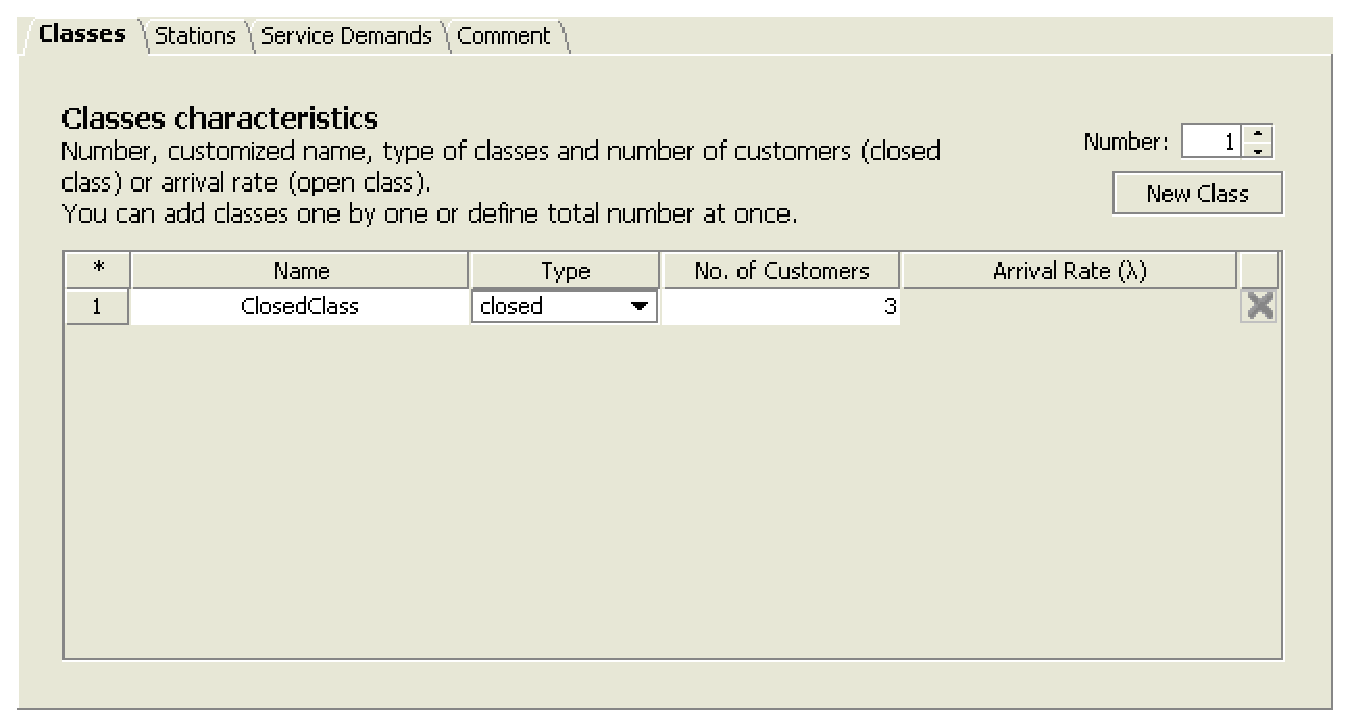
\includegraphics[scale=.5]{img/jmva/example1Class}
    \end{center}
    \caption{Example 1 - input data (Classes Tab)}
    \label{fig:jmva:example1Classes}
\end{figure}

\subsubsection{Step 2 - Stations Tab}
\begin{itemize*}
\item use \texttt{Next $>$} command to switch to \texttt{Stations Tab}
\item digit number 4 into stations number textbox or select number
4 using spin controls or push \emph{New Station} button three times.
Now your model has four \texttt{Load Independent} stations with a
default name
\item if you want you can change station names. Substitute \emph{CPU} for
default name \emph{Station1}, substitute \emph{Disk1} for default
name \emph{Station2}, substitute \emph{Disk2} for default name
\emph{Station3} and substitute \emph{Users} for default name
\emph{Station4}
\item change the type of last inserted station; \emph{Users} station is a
\texttt{Delay (Infinite Server)}
\end{itemize*}

At the end of this step, the \texttt{Stations Tab} should look like
\autoref{fig:jmva:example1Stations}.

\begin{figure}[htbp]
    \begin{center}
        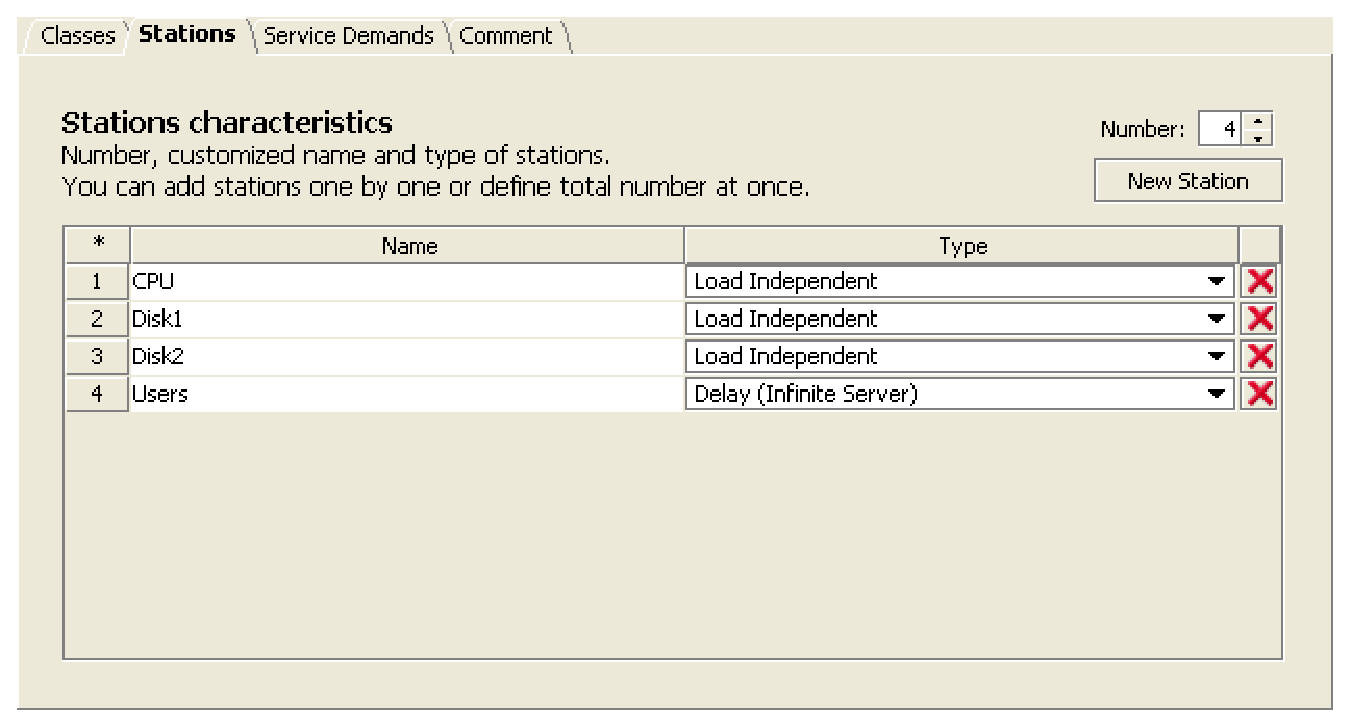
\includegraphics[scale=.5]{img/jmva/example1Stations}
    \end{center}
    \caption{Example 1 - input data (Stations Tab)}
    \label{fig:jmva:example1Stations}
\end{figure}

\subsubsection{Step 3 - Service Times and Visits Tabs}
\begin{itemize*}
\item use \texttt{Next $>$} command to switch to \texttt{Service Demands Tab}
\item press \emph{Service Time and Visit} button as you don't know
the Service Demands of the three stations: in this case Service
Times and number of Visits should be typed. After button pressure,
the \texttt{Service Demands Tab} will be hidden and \texttt{Service
times Tab} and \texttt{Visit Tab} will appear
\item you can input all Service Times in the table.
Remember that Service Time of the \emph{Users} station, of delay
type, is \emph{think time} $Z$, in this case $16$ s
\end{itemize*}

At this point, the \texttt{Service Times Tab} should look like
\autoref{fig:jmva:example1Service}.

\begin{figure}[htbp]
    \begin{center}
        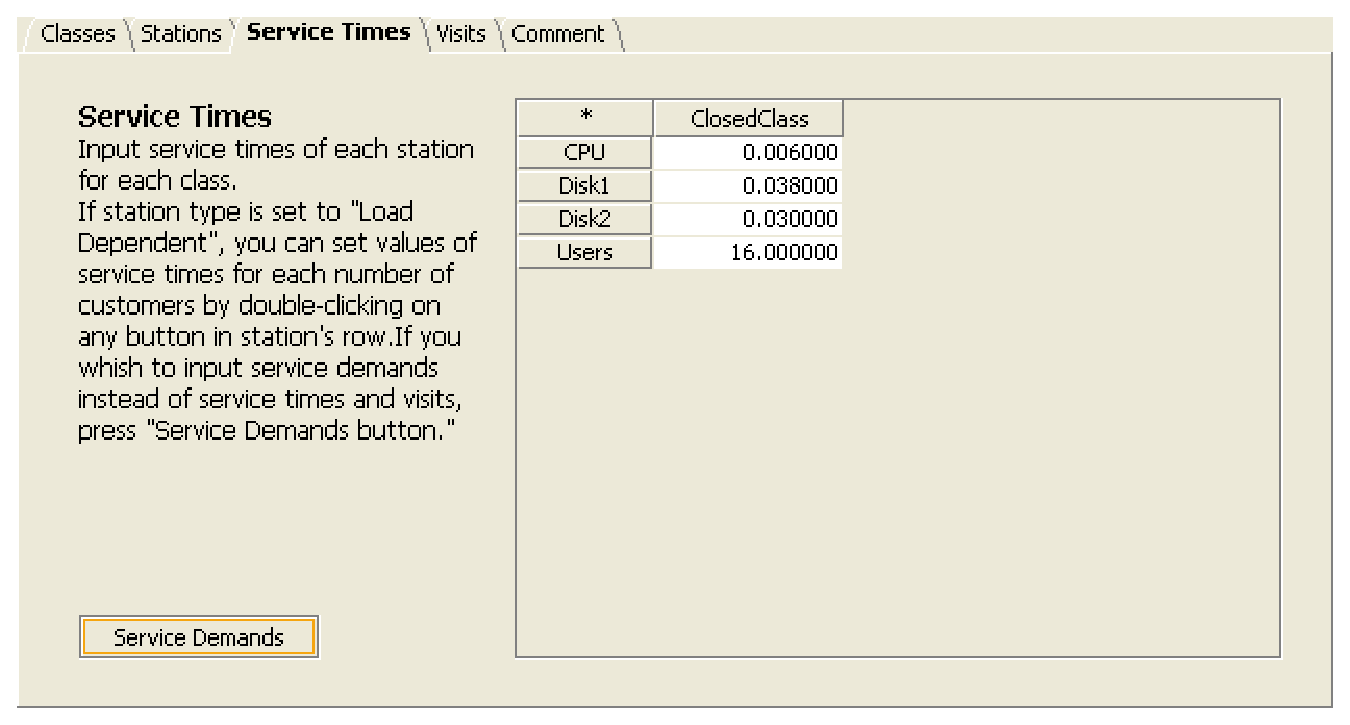
\includegraphics[scale=.5]{img/jmva/example1Service}
    \end{center}
    \caption{Example 1 - input data (Service Times Tab)}
    \label{fig:jmva:example1Service}
\end{figure}

\begin{itemize*}
\item use \texttt{Next $>$} command to switch to \texttt{Visits Tab}
\item input numbers of visits for all centers in the
table. In this case the number of visits of the \emph{Users}, the
infinite server station, is equal to 1 since a customer at the end
of an interaction with the system visits this station.
\end{itemize*}

At the end of this step, the \texttt{Visits Tab} looks like
\autoref{fig:jmva:example1Visits}.

\begin{figure}[htbp]
    \begin{center}
        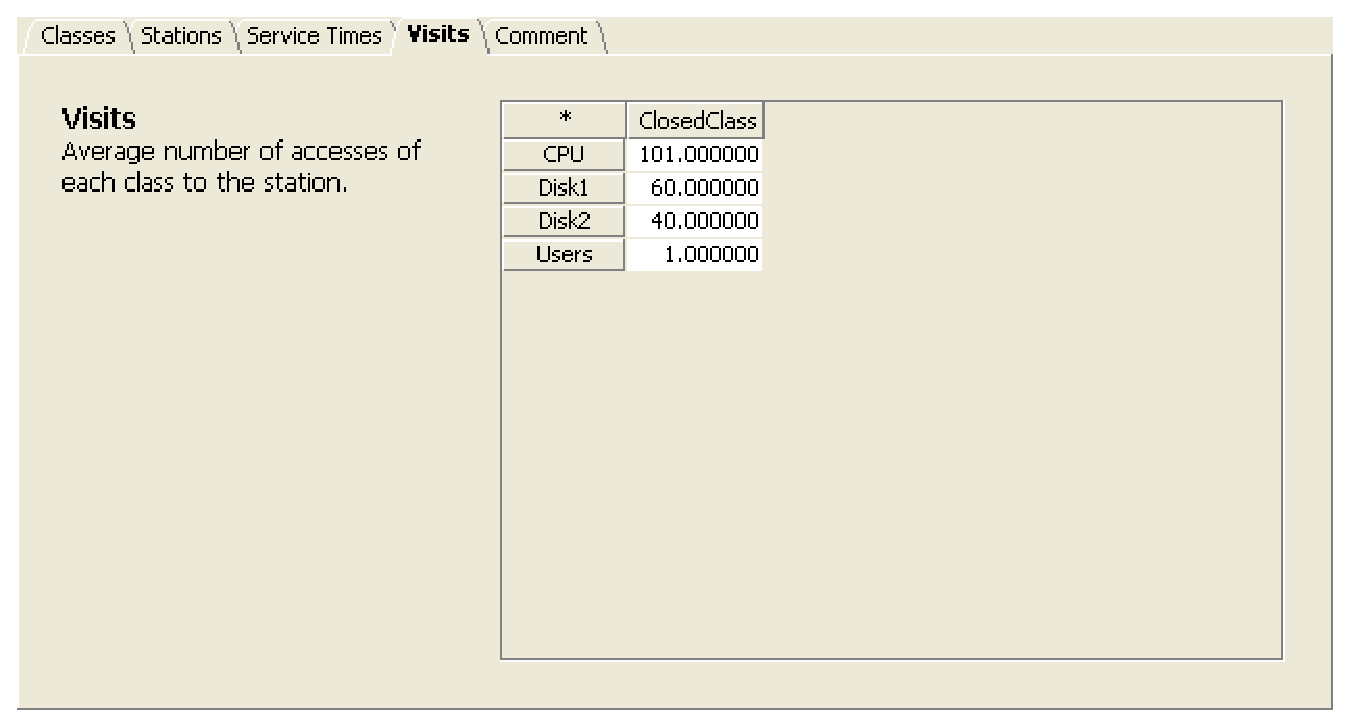
\includegraphics[scale=.5]{img/jmva/example1Visits}
    \end{center}
    \caption{Example 1 - input data (Visits Tab)}
    \label{fig:jmva:example1Visits}
\end{figure}

\subsubsection{Step 4 - Model Resolution}

Use \texttt{Solve} command to start the solution of the input model.
Model results will be displayed in a new window like the one of
\autoref{fig:jmva:example1Throughput}.

\begin{figure}[htbp]
    \begin{center}
        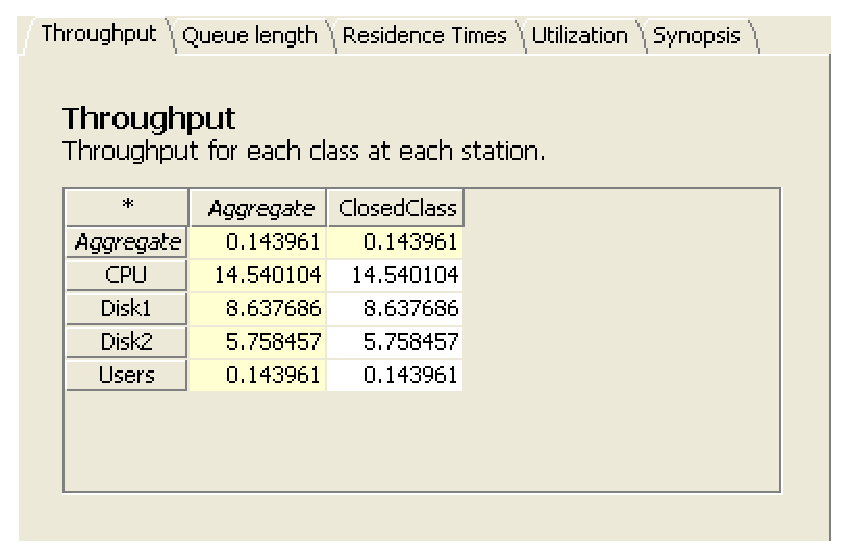
\includegraphics[scale=.5]{img/jmva/example1throughput}
    \end{center}
    \caption{Example 1 - output data (Throughput Tab)}
    \label{fig:jmva:example1Throughput}
\end{figure}

Since we are considering a single-class model, all results in the
column \emph{Aggregate} correspond to the results in the
\emph{ClosedClass} column.

JMVA computes Residence Times $W_k$, Throughputs $X_k$, Queue
lengths $Q_k$ and Utilizations $U_k$ for all stations. The algorithm
begins with the known solution for the network with zero customers,
and iterates on $N$ that, in this example, is three. Note that the
aggregate \emph{Residence Time} is the \emph{System Response Time}
measure and the aggregate \emph{Queue Length} is the average number
of customers in the system.

Using tab selector, you can change tab and see Queue length,
Residence Times, Utilizations and a synopsis panel with a schematic
report of the model (\autoref{fig:jmva:example1results}).

\begin{figure}[htbp]
    \begin{center}
        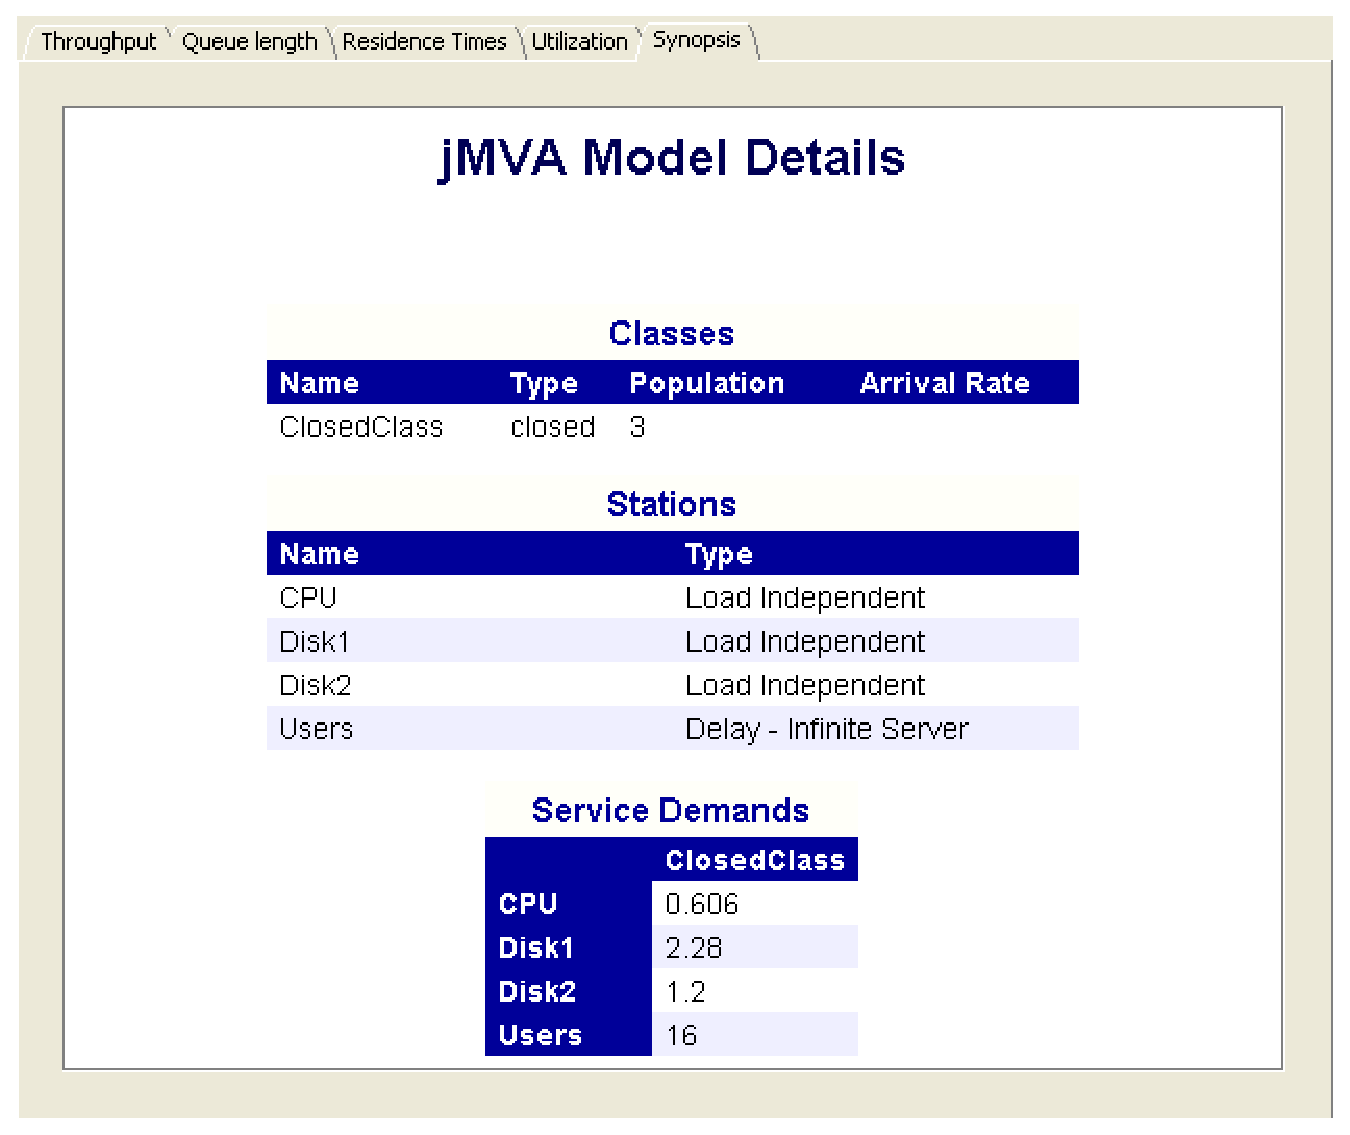
\includegraphics[scale=.5]{img/jmva/example1results}
    \end{center}
    \caption{Example 1 - output data (Synopsis Tab)}
    \label{fig:jmva:example1results}
\end{figure}

The computed performance indices are shown in
\autoref{tab:jmva:example1results}.

\begin{table}[htbp]
\begin{center}
\begin{tabular}{c|r|r|r|r|r|}
& \multicolumn{1}{c|}{Aggregate} & \multicolumn{1}{c|}{CPU} & \multicolumn{1}{c|}{Disk1} & \multicolumn{1}{c|}{Disk2} & \multicolumn{1}{c|}{Users}\\
\hline
Throughput [job/s]& $0.144$ & $14.540$ & $8.637$ & $5.758$ & $0.144$\\
Queue Length [job]& $3.000$ & $0.193$ & $0.410$ & $0.194$ & $2.303$\\
Residence Time [s]& $20.839$ & $0.643$ & $2.847$ & $1.349$ & $16.000$\\
Utilization & \multicolumn{1}{c|}{-} & $0.087$ & $0.328$ & $0.172$ & $2.303$\\
\hline
\end{tabular}
\end{center}
\caption{Example 1 - model outputs} \label{tab:jmva:example1results}
\end{table}


\subsection{Example 2 - A model with two open classes}
\label{sec:jmva:example2} Solve the multiclass open model specified
in \autoref{fig:jmva:Example2topology}.
\begin{figure}[htbp]
    \begin{center}
        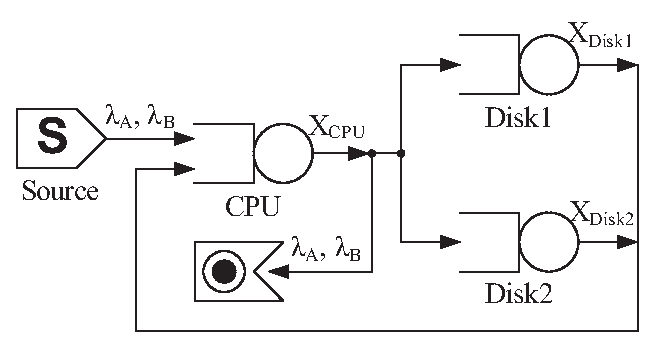
\includegraphics[scale=.65]{img/jmva/example2}
    \end{center}
    \caption{Example 2 - network topology}
    \label{fig:jmva:Example2topology}
\end{figure}
The model is characterized by two open classes $A$ and $B$ with
arrival rate (the workload intensity $\lambda$) respectively of
$\lambda_A = 0.15$ job/s and $\lambda_B=0.32$ job/s. There are three
stations of load independent type, identified with names \emph{CPU},
\emph{Disk1} and \emph{Disk2}. Service times and visits for stations
are shown in \autoref{tab:jmva:example2ServTimes} and
\autoref{tab:jmva:example2Visits}.

\begin{table}[htbp]
\begin{center}
\begin{tabular}{c|r|r|r|r|}
& \multicolumn{1}{c|}{CPU} & \multicolumn{1}{c|}{Disk1} & \multicolumn{1}{c|}{Disk2} \\
\hline
Class $A$ [s]& $0.006$ & $0.038$ & $0.030$ \\
Class $B$ [s]& $0.014$ & $0.062$ & $0.080$ \\
\hline
\end{tabular}
\end{center}
\caption{Example 2 - service times}
\label{tab:jmva:example2ServTimes}
\end{table}

\begin{table}[htbp]
\begin{center}
\begin{tabular}{c|r|r|r|r|}
& \multicolumn{1}{c|}{CPU} & \multicolumn{1}{c|}{Disk1} & \multicolumn{1}{c|}{Disk2} \\
\hline
Class $A$ & $101.0$ & $60.0$ & $40.0$ \\
Class $B$ & $44.0$ & $16.0$ & $27.0$ \\
\hline
\end{tabular}
\end{center}
\caption{Example 2 - number of visits}
\label{tab:jmva:example2Visits}
\end{table}

Since this model is similar to the network of
\autoref{fig:jmva:Example1topology} solved in
\autoref{sec:jmva:example1}, we will show how to easily create it
from a saved copy of Example~1:
\begin{enumerate*}
    \item Open the saved instance of Example~1 model
    \item Go to \texttt{Classes Tab}, change \emph{ClosedClass} name
    to \emph{A}, change its type to \texttt{Open} and set its arrival
    rate to $\lambda_A = 0.15$ job/s.
    \item Click on \emph{New Class} button, sets name of new class to
    \emph{B}, change its type to \texttt{Open} and set its arrival
    rate to $\lambda_B = 0.32$ job/s.
    \item Go to \texttt{Stations Ta}b and remove \emph{Users} delay
    center.
    \item Go to \texttt{Service Times Tab} and sets service times for
    Class $B$ according to \autoref{tab:jmva:example2ServTimes}.
    \item Go to \texttt{Visits Tab} and sets visits for
    Class $B$ according to \autoref{tab:jmva:example2Visits}.
    \item Select \texttt{Solve} action.
\end{enumerate*}

The \texttt{Synopsis Tab} with a schematic report of the model
created is shown on \autoref{fig:jmva:example2results}, while the
computed performance indices of this model are shown in
\autoref{tab:jmva:example2results}.

\begin{figure}[htbp]
    \begin{center}
        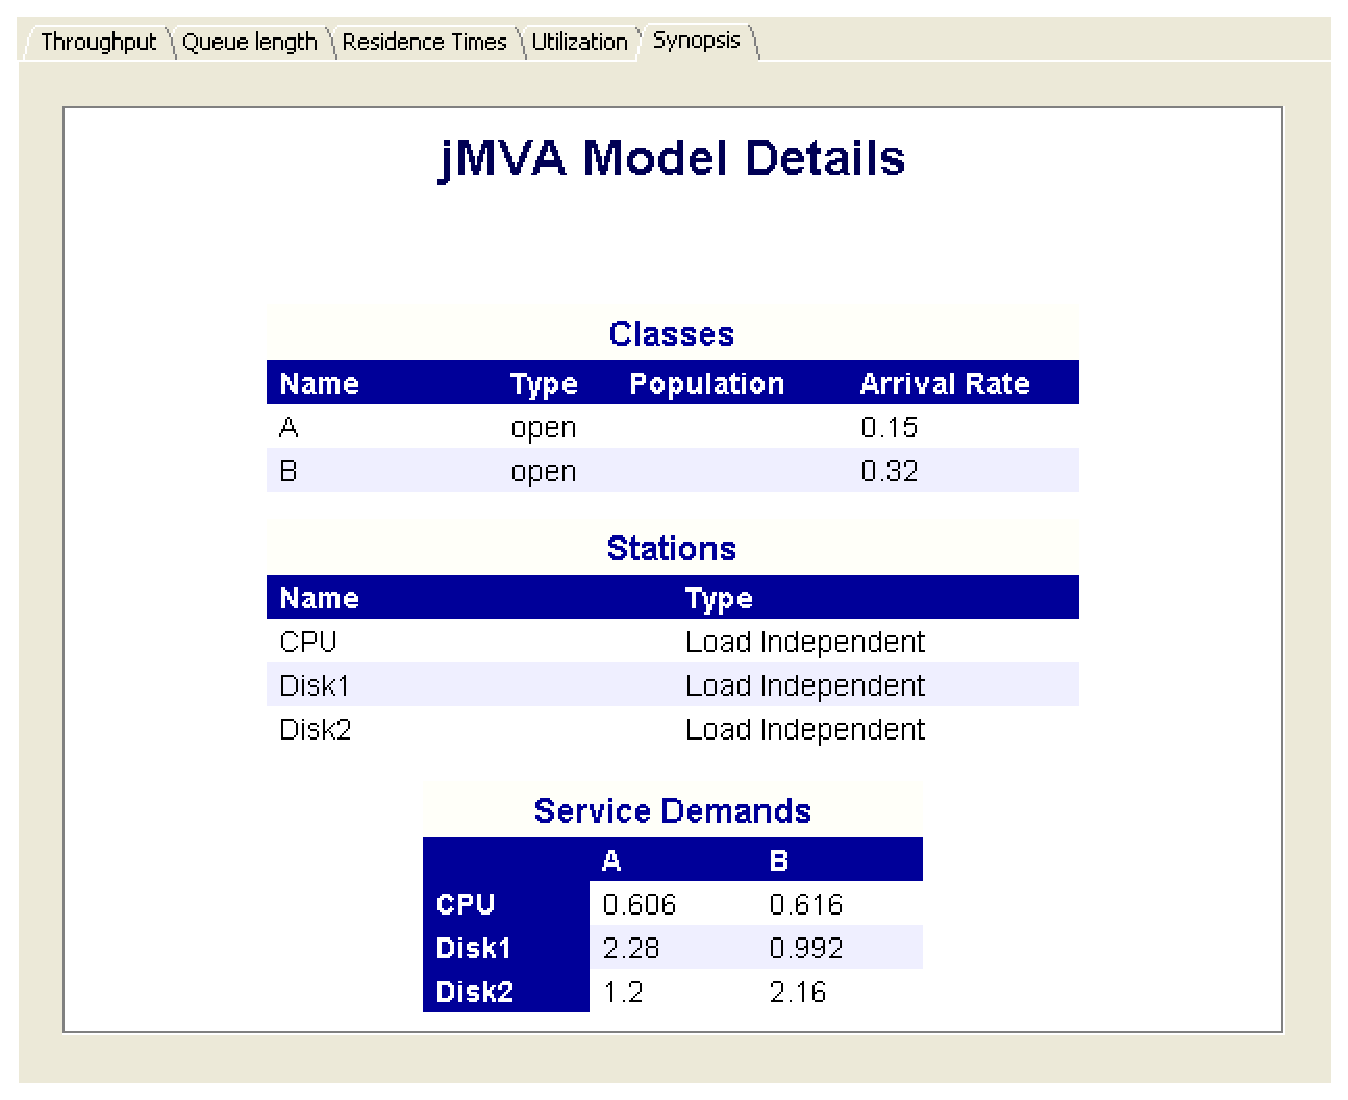
\includegraphics[scale=.5]{img/jmva/example2results}
    \end{center}
    \caption{Example 2 - output data (Synopsis Tab)}
    \label{fig:jmva:example2results}
\end{figure}

\begin{table}[htbp]
\begin{center}
\begin{tabular}{c|r|r|r|r|}
&\multicolumn{4}{c|}{Class $A$}\\
& \multicolumn{1}{c|}{Aggregate} & \multicolumn{1}{c|}{CPU} & \multicolumn{1}{c|}{Disk1} & \multicolumn{1}{c|}{Disk2}\\
\hline Throughput [job/s]& $0.150$ & $15.150$ & $9.000$ & $6.000$\\
Queue Length [job]& $2.529$ & $0.128$ & $1.004$ & $1.398$\\
Residence Time [s]& $16.863$ & $0.851$ & $6.695$ & $9.317$\\
Utilization & \multicolumn{1}{c|}{-} & $0.091$ & $0.342$ & $0.180$\\
\hline \multicolumn{5}{c}{ }\\
\multicolumn{5}{c}{ }\\
&\multicolumn{4}{c|}{Class $B$}\\
& \multicolumn{1}{c|}{Aggregate} & \multicolumn{1}{c|}{CPU} & \multicolumn{1}{c|}{Disk1} & \multicolumn{1}{c|}{Disk2}\\
\hline Throughput [job/s]& $0.320$ & $14.080$ & $5.120$ & $8.640$\\
Queue Length [job]& $6.575$ & $0.277$ & $0.932$ & $5.366$\\
Residence Time [s]& $20.548$ & $0.865$ & $2.913$ & $16.770$\\
Utilization & \multicolumn{1}{c|}{-} & $0.197$ & $0.317$ & $0.691$\\
\hline
\end{tabular}

\end{center}
\caption{Example 2 - model outputs} \label{tab:jmva:example2results}
\end{table}

\subsection{Example 3 - A model with a load dependent station}
\label{sec:jmva:example3} The network is shown in
\autoref{fig:jmva:Example3topology}.
\begin{figure}[htbp]
    \begin{center}
        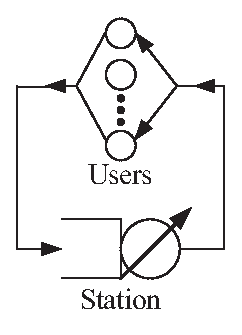
\includegraphics[scale=.65]{img/jmva/example3}
    \end{center}
    \caption{Example 3 - network topology}
    \label{fig:jmva:Example3topology}
\end{figure}
It comprises only two stations: one is of delay type (named
\emph{Users}) and the other is a load dependent station (named
\emph{Station}). This model has one closed class only with $N=8$
customers. The user's \emph{think time} is $Z = 21$ s, while the
service demands for the load dependent \emph{Station}, shown in
\autoref{tab:jmva:example3ServDemands}, are function of $n$: number
of customers in the station ($D(n) = n + 1/n$).

\begin{table}[htbp]
\begin{center}
\begin{tabular}{c|c|c|c|c|c|c|c|c|}
$n$ & $1$ & $2$ & $3$ & $4$ & $5$ & $6$ & $7$ & $8$\\
\hline
$D(n)$ [s] & $2.00$ & $2.50$ & $3.33$ & $4.25$ & $5.20$ & $6.17$ & $7.14$ & $8.13$ \\
\hline
\end{tabular}
\end{center}
\caption{Example 3 - service demands for \emph{Station}, a
load-dependent service center} \label{tab:jmva:example3ServDemands}
\end{table}

\subsubsection{Step 1 - Classes Tab}

The instructions that are the same given in Step 1 of
\autoref{sec:jmva:example1}; in this case $N$ must be 8.

\subsubsection{Step 2 - Stations Tab}

The instructions are given in Step 2 of \autoref{sec:jmva:example1};
in this case the model has two stations: a Load Dependent station
and a Delay Center.

\subsubsection{Step 3 - Service Demands Tab}

\begin{enumerate*}
\item use \texttt{Next $>$} command to switch to \texttt{Service Demands Tab}
\item double-click on cell with text \emph{LD Setting\dots}
to open the editor of load dependent service demands in a separate
window, shown in \autoref{fig:jmva:example3ldBefore}.
\item it is not mandatory to insert all values one-by-one. You can
click or drag to select cells, enter the expression $n + 1/n$ into
the textbox at the bottom of the window and click the
\emph{Evaluate} button.
\item at the end of this phase, editor window looks like
\autoref{fig:jmva:example3ldAfter}. Now you may press \emph{OK}
button to confirm changes and return to JMVA main window.
\end{enumerate*}

\begin{figure}[htbp]
    \begin{center}
        \includegraphics[scale=.5]{img/jmva/example3ldBefore}
    \end{center}
    \caption{Example 3 - editor for the description of service
    demands for a load dependent station corresponding to the different number of
    customers before the parametrization}
    \label{fig:jmva:example3ldBefore}
\end{figure}

\begin{figure}[htbp]
    \begin{center}
        \includegraphics[scale=.5]{img/jmva/example3ldAfter}
    \end{center}
    \caption{Example 3 - editor for the description of service
    demands for a load dependent station. In this case an arithmetic function
    has been defined: $S(n)=n+1/n$}
    \label{fig:jmva:example3ldAfter}
\end{figure}

\subsubsection{Step 4 - Model Resolution}

Use \texttt{Solve} command to resolve the model, results are shown
in \autoref{tab:jmva:example4results}.

\begin{table}[htbp]
\begin{center}
\begin{tabular}{c|r|r|r|r|r|}
& \multicolumn{1}{c|}{Aggregate} & \multicolumn{1}{c|}{Station} & \multicolumn{1}{c|}{Users}\\
\hline
Throughput [job/s] & $0.234$ & $0.234$ & $0.234$ \\
Queue Length [job]& $8.000$ & $3.080$ & $4.920$ \\
Residence Time [s]& $34.149$ & $13.149$ & $21.000$ \\
Utilization & \multicolumn{1}{c|}{-} & $0.810$ & $0.973$ \\
\hline
\end{tabular}
\end{center}
\caption{Example 4 - model outputs} \label{tab:jmva:example4results}
\end{table}

\subsection{Example 4 - A model with one open and one closed class}
\label{sec:jmva:example4}

The mixed queueing network model is shown in
\autoref{fig:jmva:Example4topology}.
\begin{figure}[htbp]
    \begin{center}
        \includegraphics[scale=.65]{img/jmva/example4}
    \end{center}
    \caption{Example 4 - network topology}
    \label{fig:jmva:Example4topology}
\end{figure}
Workload intensities: the open class has an arrival rate $\lambda =
1$ job/s, the closed class has a customers number $N = 57$. Service
demands are shown in \autoref{tab:jmva:example4ServDemands}.

\begin{table}[htbp]
\begin{center}
\begin{tabular}{c|r|r|r|r|}
& \multicolumn{1}{c|}{Station1} & \multicolumn{1}{c|}{Station2} & \multicolumn{1}{c|}{Station3} \\
\hline
OpenClass [s]& $0.5$ & $0.8$ & $0.6$ \\
ClosedClass [s]& $10.0$ & $4.0$ & $8.0$ \\
\hline
\end{tabular}
\end{center}
\caption{Example 4 - service demands}
\label{tab:jmva:example4ServDemands}
\end{table}

\subsubsection{Step 1 - Classes Tab}

Follow the instructions of Step~1 in the previous examples; the
\texttt{Classes Tab} is shown in \autoref{fig:jmva:example4Class}.

\begin{figure}[htbp]
    \begin{center}
        \includegraphics[scale=.5]{img/jmva/example4Class}
    \end{center}
    \caption{Example 4 - Class Tab}
    \label{fig:jmva:example4Class}
\end{figure}

\subsubsection{Step 2 - Stations Tab}

Follow the instructions of Step~2 in the previous examples; in this
case the model has three Load Independent stations (see
\autoref{fig:jmva:example4Stations}).

\begin{figure}[htbp]
    \begin{center}
        \includegraphics[scale=.5]{img/jmva/example4Stations}
    \end{center}
    \caption{Example 4 - Stations Tab}
    \label{fig:jmva:example4Stations}
\end{figure}

\subsubsection{Step 3 - Service Demands Tab}

Follow the instructions of Step~3 in the previous examples and
define service demands for both classes as illustrated in
\autoref{tab:jmva:example4ServDemands} (see
\autoref{fig:jmva:example4Services}).

\begin{figure}[htbp]
    \begin{center}
        \includegraphics[scale=.5]{img/jmva/example4Services}
    \end{center}
    \caption{Example 4 - Service Demands Tab}
    \label{fig:jmva:example4Services}
\end{figure}

\subsubsection{Step 4 - Model Solution}
Use \texttt{Solve} command. Results can be verified by computing the
\emph{equivalent model}, where the open class ``slows down'' the
closed class by subtracting utilization to it:

\begin{eqnarray*}
D_{1}^{eq}&=&\frac{D_{1,ClosedClass}}{1- \lambda * D_{1,OpenClass}} = 20 s\\
D_{2}^{eq}&=&\frac{D_{2,ClosedClass}}{1- \lambda * D_{2,OpenClass}} = 20 s\\
D_{3}^{eq}&=&\frac{D_{3,ClosedClass}}{1- \lambda * D_{3,OpenClass}} = 20 s\\
\end{eqnarray*}

MVA algorithm is used to solve the equivalent closed model. The
number of customers of the closed class is $57$, and the exact MVA
technique should require the solution of other $56$ models with
smaller population. In this particular case, the formula used to
compute the throughput can be simplified because the Service Demands
are all equals:

\begin{eqnarray*}
X^{eq}(N)&=&\frac{N}{\sum_{k=1}^{3} D_{k}^{eq} + \sum_{k=1}^{3}
\left[D_{k}^{eq}*Q_{k}^{eq}(N-1)\right]}\\
&=&\frac{N}{60 + 20*\sum_{k=1}^{3}
Q_{k}^{eq}(N-1)}\\
&=&\frac{N}{60 + 20*(N-1)}\\
\\
\\
X^{eq}(57)&=&0.048305 \textrm{ job/s}
\end{eqnarray*}

So the throughput measure for the closed class is $X_{ClosedClass} =
X^{eq} = 0.048305$ job/s while the throughput for the open class
coincide with its arrival rate $X_{OpenClass} = \lambda$. As visits
were not specified, they have been considered equal to one: that's
why throughput is equal at each station for each class (see
\autoref{fig:jmva:example4Throughput}), i.e. the solved model
consists of 3 stations that are sequentially connected with
feedback.

\begin{figure}[htbp]
    \begin{center}
        \includegraphics[scale=.5]{img/jmva/example4Throughput}
    \end{center}
    \caption{Example 4 - throughput}
    \label{fig:jmva:example4Throughput}
\end{figure}

Queue lenghts can be computed with the following formulas:
\begin{eqnarray*}
Q_{k,ClosedClass}(N)&=&Q_k^{eq}(N)\\
Q_{k,OpenClass}(N)&=&\frac{\lambda*D_{k,OpenClass}*\left[1+Q_{k,ClosedClass}(N)\right]}{1-\lambda*D_{k,OpenClass}}
\end{eqnarray*}

And the results will be equal to the ones shown in
\autoref{fig:jmva:example4Queue}.

\begin{figure}[htbp]
    \begin{center}
        \includegraphics[scale=.5]{img/jmva/example4Queue}
    \end{center}
    \caption{Example 4 - queue lengths}
    \label{fig:jmva:example4Queue}
\end{figure}

\subsection{Example 5 - Find optimal Population Mix values}
\label{sec:jmva:example5} Perform a what-if analysis to find the
value of population mix that will maximize \texttt{System
Throughput} and minimize \texttt{System Response Time} in the model
shown in \autoref{fig:jmva:Example5topology}.
\begin{figure}[htbp]
    \begin{center}
        \includegraphics[scale=.65]{img/jmva/example5}
    \end{center}
    \caption{Example 5 - network topology}
    \label{fig:jmva:Example5topology}
\end{figure}
This model has two closed classes (named \emph{Class1} and
\emph{Class2}) with a total population of $N=20$ and three load
independent stations (named \emph{Station1}, \emph{Station2} and
\emph{Station3}) with the service demands shown in
\autoref{tab:jmva:example5ServDemands}.

\begin{table}[htbp]
\begin{center}
\begin{tabular}{c|r|r|r|r|}
& \multicolumn{1}{c|}{Station1} & \multicolumn{1}{c|}{Station2} & \multicolumn{1}{c|}{Station3} \\
\hline
Class1 [s]& $1.0$ & $5.0$ & $1.0$ \\
Class2 [s]& $5.0$ & $1.0$ & $5.0$ \\
\hline
\end{tabular}
\end{center}
\caption{Example 5 - service demands}
\label{tab:jmva:example5ServDemands}
\end{table}

\subsubsection{Step 1 - Classes Tab}

Follow the instructions of Step~1 in the previous examples; as we
will change population mix, initial allocation of the $N=20$ jobs is
irrelevant. For example we can allocate $N_1=10$ jobs to
\emph{Class1} and $N_2=10$ jobs to \emph{Class2}. The
\texttt{Classes Tab} is shown in \autoref{fig:jmva:example5Class}.

\begin{figure}[htbp]
    \begin{center}
        \includegraphics[scale=.5]{img/jmva/example5Class}
    \end{center}
    \caption{Example 5 - Class Tab}
    \label{fig:jmva:example5Class}
\end{figure}

\subsubsection{Step 2 - Stations Tab}

Follow the instructions of Step~2 in the previous examples; in this
case the model has three Load Independent stations (see
\autoref{fig:jmva:example5Stations}).

\begin{figure}[htbp]
    \begin{center}
        \includegraphics[scale=.5]{img/jmva/example5Stations}
    \end{center}
    \caption{Example 5 - Stations Tab}
    \label{fig:jmva:example5Stations}
\end{figure}

\subsubsection{Step 3 - Service Demands Tab}

Follow the instructions of Step~3 in the previous examples and
define service demands for both classes as illustrated in
\autoref{tab:jmva:example5ServDemands} (see
\autoref{fig:jmva:example5Services}).

\begin{figure}[htbp]
    \begin{center}
        \includegraphics[scale=.5]{img/jmva/example5Services}
    \end{center}
    \caption{Example 5 - Service Demands Tab}
    \label{fig:jmva:example5Services}
\end{figure}

\subsubsection{Step 4 - What-if Tab}
\begin{enumerate*}
    \item use \texttt{Next $>$} command to switch to \texttt{What-if Tab}
    \item Select \texttt{Population Mix} as a \emph{control parameter} of
    the analysis in the combo box, several fields will be shown below.
    \item \emph{Class1} is already selected, by default, as reference class for the what-if
    analysis. This means that $\beta_i$ values in \texttt{From} and
    \texttt{To} fields are referred to \emph{Class1}.
    \item By default, JMVA suggests the minimum allowed value of $\beta_1$
    in the \texttt{From} field and its the maximum value in the \texttt{To}
    field\footnote{Since it is requested that one class has at least one job and customer
    number must be integer, the minimum value is $1 / N$ and the maximum value is $(N-1)/N$.}.
    Since we want to find the optimal value in the entire
    interval, we leave this unchanged.
    \item we want to perform the maximum number of allowed
    executions, so we enter a big number in the \texttt{Steps} field ($100$ for
    example). JMVA will automatically calculate the maximum number
    of allowed executions provided that number of customers for each
    class must be an integer and will report $19$.
\end{enumerate*}
At the end of this phase, the What-if Tab will look like
\autoref{fig:jmva:example5Whatif}.

\begin{figure}[htbp]
    \begin{center}
        \includegraphics[scale=.5]{img/jmva/example5Whatif}
    \end{center}
    \caption{Example 5 - What-if Tab}
    \label{fig:jmva:example5Whatif}
\end{figure}


\subsubsection{Step 5 - Model Solution}
Use \texttt{Solve} command. In the \texttt{Graphical Results Tab}
select \texttt{System Response Time} and \texttt{System Throughput}
as \emph{Performance Index}
(\autoref{fig:jmva:example5SystemResponse} and
\autoref{fig:jmva:example5SystemThroughput}). Zooming on the plot,
allows to identify the maximum value of System Throughput ($0.32$
job/s) and the minimum value of System Response Time ($62.50$ s).
They both corresponds to the execution with population mix $\beta_1
= 0.40$ for \emph{Class1}, which means that the optimal population
values are $N_1 = 8$ and $N_2 = 12$.

\begin{figure}[htbp]
    \begin{center}
        \includegraphics[scale=.5]{img/jmva/example5SystemResponse}
    \end{center}
    \caption{Example 5 - System Response Time}
    \label{fig:jmva:example5SystemResponse}
\end{figure}

\begin{figure}[htbp]
    \begin{center}
        \includegraphics[scale=.5]{img/jmva/example5SystemThroughput}
    \end{center}
    \caption{Example 5 - System Throughput}
    \label{fig:jmva:example5SystemThroughput}
\end{figure}

\chapter{JSIM\emph{wiz}}
\label{cha:jsimwiz}
\section{Overview}
Simulation can be applied when the characteristics of
the network to be analyzed make analytical techniques no
longer useful for its performance evaluation. A simulator is a
dynamic model able to follow the evolution in time of both the
system complexity it represents and the pattern of arrival
requests to be executed.\\
In the JMT \emph{suite} a discrete-event simulator JSIM for the
analysis of queueing network models is provided. It can be used
through two interfaces: alphanumerical (JSIM\emph{wiz}) and
graphical (JSIM\emph{graph}). \textbf{The manual of
JSIM\emph{graph} is more detailed than this one. If
some information are omitted or unclear in the present manual you
may consult it.}

An intuitive user interface allows even an unexperienced user to
build with JSIM\emph{wiz} system models with sophisticated
characteristics. It helps the users to perform an evaluation study
in two ways. Firstly, critical statistical decisions, such as
transient detection and removal, variance estimation, and
simulation length control, have been \emph{completely automated},
thus freeing the users from taking decisions about parameters s/he
may not be familiar with. The simulation is automatically stopped
when all performance indexes can be estimated with the required
accuracy. Secondly, a user-friendly graphical interface allows the
user to describe, both the network layout and the input
parameters. Furthermore, the graphical interface also provides
support for the use of advanced features (several of them are for
networks with very general characteristics, usually referred to as
\emph{non-product-form} networks) like fork and join of customers,
blocking mechanisms, regions with capacity constraints on
population, state-dependent routing strategies, user-defined
general distributions, import and reuse of log data. A module for
\emph{What-If Analysis}, where a sequence of simulations is run
for different values of control parameters, particularly useful in
capacity planning, tuning and optimization studies, is also
provided.

The simulation engine performs on-line the statistical analysis of
measured performance indices, plots the collected values, discards
the initial
transient periods and computes the confidence intervals.\\
All the plots generated by a simulation can be exported in vector
(e.g., eps, pdf) or raster (e.g., jpeg,
png) image formats.\\

\ \\
\noindent \textbf{\large Main Features}\\
\noindent \textbf{Arrival rates} for open classes of customers
generated by Source stations and station \emph{service times} (for
any type of station in open and closed models) can be generated
according to the following distributions: Burst (general), Burst (MMPP2),
Constant, Erlang, Exponential, Gamma, Hyperexponential, Normal,
Pareto, Poisson, Student-T, Uniform \\

\noindent \textbf{Queueing discipline}: the following strategies
are available:  First Come First Served, FCFS with priority, Last
Come First Served, LCFS with priority\\

\noindent \textbf{Routing} of the customers in the network, i.e.,
the path followed by the requests among the resources, can be
described either probabilistically or according to the following
strategies: Fastest service, Least utilization, Random, Round
robin, Join the Shortest Queue, Shortest response time (the values
of the control parameters are evaluated on the stations connected
in output to the considered one). These strategies can be further
combined among themselves through the use of a \emph{routing
station}.\\

\noindent \textbf{Other peculiar features} of the simulator are:
\vspace{-0.2cm}
\begin{itemize*}
    \item Load dependent service time strategies
    \item Fork-and-join stations to model parallelism
    \item Simulation of complex traffic pattern and service times (e.g., burst)
    \item Blocking regions (in which the number of customer is limited)
    \item What-if analysis (with various control parameters)
    \item Customization of default values
    \item Import/Export of the model from/to JMVA, the exact solver (when
    the required analytic assumptions are satisfied)
    \item Logging of the job flows in any part of the model
    (\emph{Logger} station)
    \item Graphical visualization of the evaluated performance
    indices together with their confidence intervals
    \item automatic transient detection and removal
    \item automatic stop of the simulation when all performance
    metrics can be estimated with the required accuracy.
\end{itemize*}
JSIM\emph{wiz} has a modular Java-based architecture that allows
the introduction of new Java classes in the simulation engine
without any modification to the source codes of the other classes.


\subsection{Starting the discrete-event simulator}
Selecting \includegraphics[scale=.5]{img/JSIMIcon.eps} button on the
starting screen, \autoref{fig:jsim:Classes} window shows up.
\begin{figure}[htb]
    \begin{center}
        \includegraphics[scale=.5]{img/jsim/define_class1.eps}
    \end{center}
    \caption{The home window of JSIM\emph{wiz} simulator}
    \label{fig:jsim:Classes}
\end{figure}
Three main areas are shown:
\begin{description*}
\item[Menu :] it is organized into three groups of functions. To use a
menu, click on the menu heading and choose the appropriate option.
For the description of menu entries, see \autoref{sec:jmva:Menu}
\item[Toolbar :] contains some buttons to speed up access to JSIM functions
(e.g. New model, Open, Save\dots ). If you move the mouse pointer over a button a tooltip will be shown up.
\item[Page Area :] this is the core of the window. All JSIM parameters are grouped in
different tabs. You can modify only a subset of them by selecting
the right tab, as will be shown later.
\end{description*}

\section{Defining a new model}
\label{sec:DefiningANewModel}
To define a new model, select the New command from the File menu, or the button \includegraphics[scale=.5]{img/jsim/new.eps} or use the shortcut CTRL+N. A new model is automatically created every time JSIM is started.\\\\
The following parameters must be defined in order to complete the new model:
\begin{itemize*}
\item Classes
\item Stations
\item Connections
\item Station parameters \textbf{*}
\item Performance indices
\item Reference stations
\item Finite capacity regions \textbf{*}
\item Simulation *
\end{itemize*}
To set each parameter, follow the user manual step by step.

\noindent \textbf{NOTE:} if no values are provided for the parameters marked with \textbf{*}, default values will be used and the simulation will run anyway.

\subsection{Define Classes}
\label{sec:DefineClasses}
Customer classes identify different customer behavior and
characteristics, such as the type (closed or open), the size of the customer population (for closed classes) or the interarrival time distribution (for open classes).
They can be set using the \texttt{Classes} tab during the creation of a new model.\\
\begin{center}
\includegraphics[scale=.5]{img/jsim/define_class1}
\end{center}

\noindent\textbf{{Adding a Class}}

Classes must be explicitly added to the model, either one at a time by clicking the \includegraphics[scale=.5]{img/jsim/button_addClass.eps} button, or by selecting directly the final number of classes desired in the form \includegraphics[scale=.5]{img/jsim/button_NClass.eps}. The newly added classes will be listed with deafult parameters.\\
Double click on the default name (ClassN) to change it.\\
Each new class has a priority in the system. A smaller number indicates a lower priority. Default value is 0 and it can be changed by double clicking on the corresponding area.\\\\
\textbf{{Defining the Class Type: Open Classes}}

After adding a class and possibly changing its name and priority,
you must choose the type of customers comprising the class.
Classes are created Closed by default, so if you want an Open
class, select the type \texttt{Open} in the menu.
\begin{figure}[h!]
\begin{center}
\includegraphics[scale=.5]{img/jsim/type_class.eps}
\end{center}
\end{figure}
The class characteristics looks like this now
\begin{figure}[h!]
\begin{center}
%\includegraphics[scale=.5]{img/jsim/open_class1.eps}
\includegraphics[scale=.5]{img/jsim/open_class1.eps}
\end{center}
\end{figure}

Open classes describe customer populations that vary during time,
therefore they are best characterized by the probability
distribution of the interarrival time, rather than by a constant
number of customers. The default Interarrival Time Distribution is
exp(1) (Exponential Distribution with $\lambda$ =1).\\ To change
the Interarrival Time Distribution click the \texttt{Edit} button
\begin{center}
\includegraphics[scale=.5]{img/jsim/arrival_time_distribution1.eps}
\end{center}

The following window will appear
\begin{center}
\includegraphics[scale=.5]{img/jsim/erlang.eps}
\end{center}

Click on the \texttt{Selected Distribution} drop down menu to
choose from any of the following distributions (see
\autoref{distns}):
\begin{itemize*}
    \item Burst (General)
    \item Burst (MMPP2)
    \item Constant
    \item Erlang
    \item Exponential
    \item Gamma
    \item Hyperexponential
    \item Normal
    \item Pareto
    \item Poisson
    \item Replayer
    \item StudentT
    \item Uniform
\end{itemize*}

In each case, it is possible to configure the distribution
parameters as you wish, or use the default values. Parameters that
are related each other are automatically adjusted if one is
modified (for example,the figure shows how for an Erlang
distribution, if you set the ($\alpha$, r) pair, the (mean, c)
pair is automatically adjusted to the correct value). The Replayer
distribution allows you to provide data traces from files.
Click OK when you are done to return to Class parameters definition.\\
The final step in defining a class is the definition of the
Reference Station, i.e., that station in the model with
respect to which the performance indices will be computed.
For Open classes there is no choice since the Source station
is the unchangeable default Reference Station used to compute
System Throughput for all the Open classes.\\
\begin{center}
\includegraphics[scale=.5]{img/jsim/reference_open1.eps}
\end{center}
\ \\
\noindent \textbf{{Defining the Class Type: Closed Classes}}\\
\begin{center}
\includegraphics[scale=.5]{img/jsim/closed_class1.eps}
\end{center}

Classes are created Closed by default, so there is not need to change the Type. Priority can be changed as in the Open class case. The population size is the parameter that characterizes a Closed class. It is fixed and does not change for the entire life of the system. By default is 1 and it can be changed by clicking on the corresponding area in the class properties matrix.\\\\
The final step is to define a Reference Station for the class that will be used to compute the performance indices selected for the class. Use the Reference Station tab menu to select the Station.All stations but the sink can be used as reference station for a closed class.\\
\begin{center}
\includegraphics[scale=.5]{img/jsim/reference_closed1.eps}
\end{center}

\subsubsection{Distributions}
\label{sec:Distributions}

See \autoref{distns}


\subsection{Define stations}
\label{sec:DefineStations}
When you create a new model, you must define the Stations from the \textbf{Stations} page of the tabs menu.\\
\begin{center}
\includegraphics[scale=.5]{img/jsim/define_station1.eps}
\end{center}
You can insert one station at a time, by pressing the \includegraphics[scale=.5]{img/jsim/button_addStation.eps} button, or multiple stations all at once, by choosing the desired number in the input form \includegraphics[scale=.5]{img/jsim/button_Nstations.eps}
The added stations will be listed in the page. Various types of stations are available, the default type being \emph{server}.
If you want to remove any of the stations, select the target and press the corresponding \includegraphics[scale=.5]{img/jsim/delete.eps} delete button.
Stations are name Station1, Station2, and so on by default. If you want to assign model-relevant names, left-clik on a name to change and replace
it.
Similarly, if the default station type Server is not what you need, select from the drop down menu of each station the correct type.\\
\begin{center}
\includegraphics[scale=.5]{img/jsim/station_types.eps}
\end{center}
You can choose among the following types of station:
\begin{enumerate*}
\item \textbf{Delay station:} \includegraphics[scale=0.5]{img/jsim/delay.eps}\\
Customers that arrive at this station are delayed for the amount
of time that defines the station service time. They do not
experience any queueing, since a delay station is modelled as a
station with an infinite number of servers with identical service
time. Because customers never have to wait for service, response
time at delay stations is equal to service time, $R_i= S_i$.
Furthermore, the queue length corresponds in this case to the
number of jobs receiving service since there is no waiting in
queue: $Q_i = R_i\;X_i = S_i\;X_i = U_i$. The utilization of the
delay center represents the average number of jobs receiving
service (i.e., in think state). Delay centers are used when it is
necessary to reproduce some known average delay (with the selected
distribution).\\
In the \texttt{Station Parameters} tab menu page, you can modify:
\begin{description*}
\item[Service Section:]
in this section you can choose the service time distribution for the station.
For more information, see Service section \autoref{sec:ServiceSection}.
\item[Routing Section:]
in this section you can specify how serviced customers should be routed to the next station they will visit in the model.
For more information, see Routing section \autoref{sec:RoutingSection}.
\end{description*}
\item \textbf{Server station:} \includegraphics[scale=0.5]{img/jsim/server.eps}\\
The Server station is one of the most important components in a queuing network model. Service stations represent the service facilities of the system being modelled. A server station provides the required service to its customers. Server stations may have any (finite) number of servers. If all the servers in the service station are busy when a customer arrives at the station, the arriving customer is put in a waiting queue until its turn to receive service from the first available server is up.
The queueing discipline decides which customer is served next when a server becomes free. Therefore, the response time at server stations includes service time and
queuing time. Server stations may have more than one server. Their number is a parameter to be specified (default is 1).\\\\
In the Station Parameters tab menu page, you can modify:
\begin{description*}
\item[Queue Section:]
in this section you can choose the type of queue (finite or infinite) and the policy used to select the next customer to be served.
For more information, see Queue section \autoref{sec:QueueSection}.
\item[Service Section:]
in this section you can choose the service time distribution for the station.
For more information, see Service section \autoref{sec:ServiceSection}.
\item[Routing Section:]
in this section you can specify how serviced customers should be routed to the next station they will visit in the model.
For more information, see Routing section \autoref{sec:RoutingSection}.
\end{description*}
\item \textbf{Fork station:}
\includegraphics[scale=0.5]{img/jsim/fork.eps} A JSIM Fork station
is simply a station where jobs are split into tasks. No service is
provided, therefore there is no service time specification. Tasks
are then routed along the Fork station outgoing links. Unlike
classical queueing theory fork-join queues, a JSIM Fork station is
not associated with a join station automatically. Any combination
of server stations, finite regions, fork-join, routing stations,
etc., is possibile after a Fork station. This feature allows the
modeling of very general parallel behaviors, of which the
traditional Fork-Join one is a special case. In JSIM the classical
queueing theory Fork-Join queue behavior is obtained by connecting
the Fork station to as many Server stations as the degree of
parallelism requested, with one task per outgoing link. Each
Server station is then connected to a Join station, where the job
is recomposed. A Fork station is characterized by the forking
degree, i.e., the number of tasks routed on each one of its
outgoing links, and the capacity, i.e., the maximum number of jobs
that can be served by the station simultaneously. Therefore, the
number of sibling tasks a job is split into is given by the
product of the number of outgoing links from the Fork station
times the forking degree. Note that a finite station capacity
makes sense only when there is a join station downstream from the
fork station that can recompose the split jobs. Otherwise,
inconsistencies in the model and subsequent simulation error, such
as out-of-memory, may occur. No automatic checks are available at
the moment that can identify such critical conditions. Both the
forking degree and the capacity are section parameters to be
specified in the model. As an example, a Fork station with forking degree 1, connected to three Server stations, would split a job into 3 sibling tasks (this is a traditional Fork-Join like behavior). If no Join station is connected to any of the three Servers, a warning message is displayed since the model could quickly saturate due to the extra load (3 more jobs) created in addition to each job entering the Fork station.\\\\
In the Station Parameters page of the tabs menu,you can modify:\\
\begin{description*}
\item[Fork Section:] in this section you can choose the forking degree of a job on each outgoing link and the fork station capacity, i.e., the maximum number
of jobs that can be served in parallel by the station.
For more information, see Fork section \autoref{sec:ForkSection}.
\item[Queue Section:] in this section you can choose the type of queue (finite or infinite) of the fork station in case its capacity is finite and jobs must wait before
proceeding through the fork station.
For more information, see Queue section \autoref{sec:QueueSection}.
\end{description*}
\item \textbf{Join station:}
\includegraphics[scale=0.5]{img/jsim/join.eps}Join stations are
complementary to fork stations. In classical queueing network
theory, a task arrives at a join station from the corresponding
Fork station. In JSIM, a Join station may have incoming links from
stations other than the corresponding Fork one. A Join station has
no service time, as it is only used to recombine the tasks a job
had been previously split into and then route the job to some
other station(s). When a task arrives at a join station, it waits
until all its sibling tasks have arrived. At this time, the
original job is
recomposed and routed to the next station. If a job arrives from a station other than the corresponding Fork, i.e., a job that was not split, it is simply routed to the next station. In this case the Join station operates as a routing station.\\\\
In the Station Parameters tab menu page, you can modify:
\begin{description*}
\item[Routing Section:] in this section you can specify how serviced customers should be routed to the next station they will visit in the model.
For more information, see Routing section \autoref{sec:RoutingSection}.
\end{description*}
\item \textbf{Routing station:}
\includegraphics[scale=0.5]{img/jsim/load_splitter.eps} A routing
station is a dummy station, with service time equal 0, that is
used to create more complex and sophisticated routing strategies
by sending jobs through one or more such stations. For example, if
we wanted two thirds of the incoming traffic at station Z to be
randomly routed to either station A or B and the remaining third
to go either to station C or D, depending on the shortest queue at
the two stations, we could implement the following. Add a routing
station, Y, among Z's output stations and define random routing
for the three of them (A, B, Y).
Then connect Y to C and D and define Join the Shortest Queue routing to C and D.\\\\
In the Station Parameters tab menu page, you can modify:
\begin{description*}
\item[Routing Section:] in this section you can specify how serviced customers should be routed to the next station they will visit in the model.
For more information, see Routing section \autoref{sec:RoutingSection}.
\end{description*}
\item \textbf{Source station:}
\includegraphics[scale=0.5]{img/jsim/source.eps}
If the model comprises at least an open class, a sink and  a source stations are created by default, as they are necessary for the simulation and cannot be removed\\
\begin{center}
\includegraphics[scale=.5]{img/jsim/source_sink.eps}
\end{center}
Open classes are characterized by an infinite stream of jobs that can enter the system. Source stations are used to introduce jobs in the model. Their service time is the interarrival time of each customer class and as such, it is defined as a parameter of the class the job belongs to. The routing strategy defines the first station
a newly created job will visit. Only open class jobs can be routed from source stations.\\\\
In the Station Parameters tab menu page, you can modify:
\begin{description*}
\item[Routing Section:] in this section you can specify how newly
created customers should be routed to the next station they will
visit in the model. For more information, see Routing section
\autoref{sec:RoutingSection}.
\end{description*}
\item \textbf{Sink Station:} \includegraphics[scale=0.5]{img/jsim/sink.eps}\\
Open class customers leave the system once they have received all
the service the need. Sink stations are used to model customers
leaving the system, as they enter the sink station but do not ever
leave it. Sink stations have no parameters, only incoming
connections from one or more stations, depending upon the model.
\item \textbf{Logger station}
A logging station (i.e., \emph{logger}) reads information
flowing through it and writes it to a file.   In the simplest way,
it is a tool to understand and debug the traffic flow moving
through the interesting part(s) of the model. Place the logger
station into the model, choose the parameters, and trace the data
as it passes through the model.\\

\noindent \textbf{Set or change of the properties}\\
Double click on the \texttt{Logger Station} icon
\includegraphics[scale=.5]{img/jsimg/logger}
to open the \texttt{Editing Logger Properties} station's
configuration dialog (see \autoref{fig:deditlogg}). There are two
sections:
\texttt{Logger Section} and \texttt{Routing Section}.\\
\begin{figure}[htb]
    \begin{center}
        \includegraphics[scale=.8]{img/jsimg/logger_editFull_sm.eps}
    \end{center}
    \caption{Window for the \texttt{Logger Station} configuration.}
    \label{fig:deditlogg}
\end{figure}

\noindent{\textbf{Logger Section}}\\
The configuration properties of the \texttt{Logger Section} are:
\begin{itemize*} \item \textbf{Logging Options:}
\begin{itemize*} \item   The Logfile's name to use, either individual or merged
(Logger0.csv or global.csv, respectively). \item The information
to log (fields): Logger Name, Job Arrival Time (simulation units),
unique Job ID, defined Class ID, Interarrival time of same class,
Interarrival time of any class. These fields are found in the next
section. \end{itemize*} \item \textbf{Logfile Options:}
\begin{itemize*} \item Browse button: allows changing the directory where
logfiles are stored. \item Overwrite method to use when the
logfile exists, and a new simulation needs to overwrite the file.
Replace overwrites the file, append adds data to the end of the
file. \item Delimiter chooses the character to separate between.
\end{itemize*}
\item \textbf{Status} displays the path and file-status of the
logfile that is going to be written.
\end{itemize*}

As messages flow through the Logger from one station to another,
the following information can be logged:
\begin{itemize*} \item \texttt{Logger Name}, the name of the logger
where the message occured (e.g., \emph{Logger0}) \item \texttt{Job
arrival time}, this timestamp marks the current simulation time
from start of simulation (not seconds) \item \texttt{Job ID}, the
auto-generated unique sequence number of the message (e.g.
1,2,3...). \item \texttt{Class ID}, the name of \emph{customer
class} of message (e.g., \emph{Class0}) \item \texttt{Interarrival
time (same class)}, is a time difference between customer of the
same class that passes through the logger \item
\texttt{Interarrival time (any class)}, is a time difference
between customers of any class that passes through the logger.
\end{itemize*}

Once a \emph{Logger} is configured, running a simulation produces
a logfile with the chosen fields. An example
of logfile output is:\\
\texttt{LOGGERNAME;TIMESTAMP;JOBID;JOBCLASS;TIMEELAPSED\_SAMECLASS;
TIMEELAPSED\_ANYCLASS\\ Logger0;0.199;1;Class0;0.000;0.199\\
Logger0;0.559;2;Class0;0.341;0.341}\\
\end{enumerate*}

\subsubsection{Fork section}
\label{sec:ForkSection} \textbf{How to define the Forking
Behavior} This section is characteristic only of fork stations. It
defines the parallelism degree of a job, in terms of the number of
tasks it is split into and how many jobs can be serviced
concurrently.

In this section you can define the station forking degree, i.e., the number of tasks created for each job arriving at the fork station, and its capacity, i.e., the maximum number of of jobs that can be in a fork-join section (when a join is present):\\
\begin{center}
\includegraphics[scale=.5]{img/jsim/fork1.eps}
\end{center}
\emph{Forking degree:} it is the number of tasks that are routed on each outgoing link of the fork station. Therefore, each job is split into (forking degree)*(number of outgoing links) tasks. By default the forking degree is 1 and it can be modified using this form:\\
\begin{center}
\includegraphics[scale=.5]{img/jsim/tasks.eps}
\end{center}
\emph{Capacity:} it is the maximum number of jobs that can be served by a fork-join
section simultaneously. It makes sense only if there is a join station matching the fork one. It can be finite, in which case once the limit is reached, jobs wait in the queue of the fork station. A job is removed from the queue and serviced (i.e., split into tasks) when a job is recomposed at the matching join station and leaves it. Capacity is defined using the form below, after checking the \emph{Finite capacity...} box:\\
\begin{center}
\includegraphics[scale=.5]{img/jsim/blocking.eps}
\end{center}

\subsubsection{Queue section}
\label{sec:QueueSection}
\textbf{How to Define the Queue Strategy}\\
The Queue section is part of the \textbf{Station Parameters} definition page; it is present only for server and fork stations.

The Queue section allows the specification of the queueing capacity (whether finite or infinite) and policy. Different classes may have different policies associated with them.
\begin{center}
\includegraphics[scale=.5]{img/jsim/queue_section1.eps}
\end{center}
\emph{Capacity:} a station can accept any customer and let them
wait in queue, in which case its capacity is considered infinite,
or it can only accept a finite number
of customers. In this case its capacity is finite, with a length to be specified in the form \includegraphics[scale=.5]{img/jsim/lenght.eps}\\\\
\emph{Queue policy:}it is the algorithm used to decide which customer to serve next. A variety of factors can contribute to the order in which customers are served, such as arrival order, priorities associated with a class, the amount of service already provided to customers, etc.

In JSIM queueing disciplines based on arrival order and priority are the only available, namely:

\begin{description*}
\item[FCFS:] under the First Come First Served queueing discipline, customers are served in the order in which they arrive at the station. If the model is exported to MVA, the following constraint is enforced in the exported model. Since all customer classes must have the same average service time at a FCFS station, the total number of visits to the station (Vc,k) is adjusted in order to comply with the constraint and at the same time allow for distinct service demands (Dc,k).
\item[FCFS (Priority):] under this policy, customers are ordered according to their arrival time but customers with higher priority jump ahead of customers with lower priority (conventionally a \emph{small} priority number = low priority). Customers with the same priority are served FCFS.
\item[LCFS:] under the Last Come First Served queueing discipline, an arriving job jumps ahead of the queue and will be served first, unless other jobs arrive before the one currently in service finishes. The LCFS discipline implemented in JSIM is not the preemptive-resume type.
\item[LCFS (Priority):] under this policy, the next customer to be served is one with the highest priority (conventionally a \emph{small} priority number = low priority), so an arriving customer can only jump ahead of the queue of the other jobs with the equal or smaller priority. Customers with the same priority are served LCFS.
\end{description*}

\subsubsection{Routing section}
\label{sec:RoutingSection} \textbf{How to Define the Routing
Strategy} The Routing section is part of the \textbf{Station
Parameters} definition page defined for all stations, except for
fork and sink stations. In the routing section, for every class
defined, you may decide how the completed jobs are routed to the
other devices connected to station for which the routing strategy
is defined.
\begin{center}
\includegraphics[scale=.5]{img/jsim/routing1.eps}
\end{center}
For each class, the routing algorithm to be used on the outgoing links of the station is selected from this menu:\\
\begin{center}
\includegraphics[scale=.5]{img/jsim/strategy.eps}
\end{center}
By clicking an algorithm, a brief explanation of the selected algorithm is shown and routing options can be specified,where necessary:
\begin{center}
\includegraphics[scale=.5]{img/jsim/routing2.eps}
\end{center}
You can choose among the following algorithms (NOTE: in each of the pictures illustrating the algorithms, the blue station implements the routing strategy to the other devices):
\begin{description*}
\item[Random:] with this strategy, jobs are routed randomly to one of the stations connected to the routing device. The outgoing links are selected with the same probability.The figure illustrates the routing strategy with 3 output links. For each link the probability to be selected is 1/3.
\begin{center}
\includegraphics[scale=.5]{img/jsim/random.eps}
\end{center}
\item[Round Robin:] with this algorithm, jobs are cyclically routed to the outgoing links according to a circular routing. As the figure shows, the first job is sent to the top station, the second job is sent to the central station, and the third job is sent to the bottom station. The next job would be sent to the top station again, and so on.
\begin{center}
\includegraphics[scale=.5]{img/jsim/round_robin.eps}
\end{center}
\item[Probabilities:] with this algorithm, you can define the routing probability for each outgoing link.The sum of all probabilities must equal 1. If the values provided do not satisfy the constraint, JSIM automatically normalizes the values before the simulation starts.
\begin{center}
\includegraphics[scale=.5]{img/jsim/probability.eps}
\end{center}
This strategy requires that you define the probability for each
output link via the panel on the bottom right of the window.
\begin{center}
\includegraphics[scale=.5]{img/jsim/prob1.eps}
\end{center}
\item[Join the Shortest Queue:] with this strategy, each job is
routed to the device that has the smallest queue length, i.e.,
number of jobs waiting, at the time the job leaves the routing
station. The figure shows a case where the queue lengths at the
devices are 3, 2, and 1 jobs, respectively, from top to bottom.
The exiting job will be routed to the bottom station, since its
queue is the shortest(1 job).
\begin{center}
\includegraphics[scale=.5]{img/jsim/Q_length.eps}
\end{center}
\item[Shortest Response Time:] with this algorithm, jobs are sent
to the station where the average response time for the job's class
is the smallest at the moment a job leaves the routing station.The
figure shows that at the time of routing, the middle station has
the smallest average response time, R, so the job will be sent to
it.
\begin{center}
\includegraphics[scale=.5]{img/jsim/R_length.eps}
\end{center}
\item[Least Utilization:] with this strategy, the destination device is chosen as the one with the smallest average utilization at the time routing is performed. In the example depicted in the picture, the top station is the least utilized, so it will receive the next job to leave the blue station.
\begin{center}
\includegraphics[scale=.5]{img/jsim/utilization.eps}
\end{center}
\item[Fastest Service:] with this strategy, a job is routed to the device with the smallest average service time, S, for the job's class. In the figure, the exiting job will be routed to the top station since it service time is the minimum among the three.
\begin{center}
\includegraphics[scale=.5]{img/jsim/S_time.eps}
\end{center}
\end{description*}

\subsubsection{Service section}
\label{sec:ServiceSection}
\textbf{How to Define the Service Strategy}
This section is present in server and delay stations.
This section allows the specification of the number of servers, for server stations, and the service time distribution, for both server and delay stations.

Delay stations are infinite servers with identical service time, therefore they only need the service time distribution. The infinite number of servers provides for equal average response time for all jobs, as no job waits in queue for service.

In this section, the load dependent or independent nature of the service time is also specified for each class in server stations:
\begin{center}
\includegraphics[scale=.5]{img/jsim/service_section1.eps}
\end{center}
The number of servers in a server station can be modified using the corresponding input area:
\begin{center}
\includegraphics[scale=.5]{img/jsim/num_servers.eps}
\end{center}
For each class, you must specify whether the service time is Load Dependent or Load Independent using this menu:
\begin{center}
\includegraphics[scale=.5]{img/jsim/load.eps}
\end{center}
A load independent service indicates that, regardless of the number of jobs that are in the station, the system will serve all jobs following a fixed policy modelled by the chosen statistical distribution.\\
For each class, the Service Time Distribution is set to Exponential with average equal to 1. It can be modified by clicking the  \includegraphics[scale=.5]{img/jsim/edit.eps} button and inserting all the required parameters from this window:
\begin{center}
\includegraphics[scale=.5]{img/jsim/erlang.eps}
\end{center}
Click the drop down menu and choose the service time distribution among the following:
\begin{itemize*}
\item Burst (General) \item Burst (MMPP2) \item Constant \item
Erlang \item Exponential \item Gamma \item Hyperexponential \item
Normal \item Pareto \item Poisson \item Replayer \item StudentT
\item Uniform
\end{itemize*}
A load dependent service time indicates that the amount of time
the server spends with each customer depends upon the current
number of customers in the station. A set of intervals for the
number of jobs in the station is specified, either by adding one
range at a time via the
\includegraphics[scale=.5]{img/jsim/add_range.eps} button or by
specifying the total number at once. Each range must them be
specified by its lower (\texttt{From}) and upper (\texttt{To})
extremes. Each such range can be associated with different service
times, as for the distribution, the mean and the coefficient of
variation, or a subset thereof. To set the parameters of a Load
Dependent service time, click the
\includegraphics[scale=.5]{img/jsim/edit.eps} button and then
specify the parameters for each added range.
\begin{center}
\includegraphics[scale=.5]{img/jsim/load_dipendent.eps}
\end{center}
For each customer number range you must specify the following parameters:
\begin{description*}
\item [Distribution:] you can choose among Burst (general), Burst
(MMPP2), Pareto, Erlang, Exponential, Hyperexponential, Poisson,
Uniform, Constant, Gamma and Normal distribution. \item [Mean:]
the mean value of each distribution is specified in the
\emph{Mean} form by double clicking on it. Insert a number or an
arithmetic expression that will be evaluated with JFEP - Java Fast
Expression Parser. For a complete list of the command supported by
JFEP you can read the \emph{Help} tab or see the JFEP web site at
http://jfep.sourceforge.net/ \item [c:] The coefficient of
variation of each distribution (when C exist) can be specified by
double clicking on the \emph{c} form. For example, in the previous
picture two policies are defined: From 1 to 4 jobs in the station,
the server will behave according to an Erlang distribution with
mean = 1 and c=0.5. For any number of jobs greater or equal to 5
in the station, the system will behave according to an Exponential
distribution with mean = 1. If you want to delete a range click
\includegraphics[scale=.5]{img/jsim/delete.eps}
\end{description*}

\subsection{Define Connections}
\label{sec:DefineConnections} The \textbf{Connections} tab allows
you to define how stations are connected with each other. In order
to create a connection from station \emph{i} to a station
\emph{j}, check the table entry (i,j) in the connection matrix
(rows identify source stations, columns identify destination
stations)
\begin{center}
\includegraphics[scale=.5]{img/jsim/connections1.eps}
\end{center}
\textbf{NOTE:} if there are open classes in the model, the Source
and Sink station automatically created by the system appear in the
connection matrix.  A \emph{Source} station may have only outgoing
links, a \emph{Sink} station may have only incoming links.
\begin{center}
\includegraphics[scale=.5]{img/jsim/sink_source_connections.eps}
\end{center}
To define a consistent model a Source station must have at
least one outgoing connection and a Sink station must have an incoming connection.\\\\
\textbf{Example 1:} if you want to connect station1 to station2 in this way \includegraphics[scale=.5]{img/jsim/es1.eps} you must check this box
\begin{center}
\includegraphics[scale=.5]{img/jsim/connection1.eps}
\end{center}
\textbf{Example2:} if you want to connect station1 to station2 in this way \includegraphics[scale=.5]{img/jsim/es2.eps} you must check this box
\begin{center}
\includegraphics[scale=.5]{img/jsim/connection2.eps}
\end{center}
\textbf{Example3:} if you want to connect station1 to itself (with a feedback loop) \includegraphics[scale=.5]{img/jsim/es3.eps} you must check this box
\begin{center}
\includegraphics[scale=.5]{img/jsim/connection3.eps}
\end{center}
\textbf{NOTE: }if connections among the stations are inconsistent, the system displays error-warning messages. For more information about connection errors, read ref{}.

\subsection{Station Parameters}
\label{sec:StationParameters}
The \textbf{Station Parameters} tab allows you to define the characteristic parameters of each station.
For each station, a different menu is presented depending upon the station type. Queuing, service, routing and forking, or subsets thereof, are the characteristics to be defined through a series of tabs. Default settings are provided that can be modified at the user's need. The Sink station does not have any parameter.
\begin{center}
\includegraphics[scale=.5]{img/jsim/station_parameters1.eps}
\end{center}
\textbf{Example }(with a server station):
\begin{center}
\includegraphics[scale=.5]{img/jsim/sub_tabs_menu.eps}
\end{center}
\textbf{NOTE:} You can find detailed information about station parameters \autoref{sec:DefineStations}.

\subsection{Define Performance Indices}
\label{sec:DefinePerformanceIndices}
Performance Indices are selected using the \textbf{Performance Indices} tab.
\begin{center}
\includegraphics[scale=.5]{img/jsim/define_indices1.eps}
\end{center}
You can choose any subset of indices from the list below to be
plotted as the model output:
\begin{description*}
\item [Queue Length] Number of customers at a station, both
waiting and receiving service. \item [Queue Time] Average time
spent by the customers waiting in a station queue. It does not
include the Service Time. \item [Residence Time] Total time spent
at a station by a customer, both queueing and receiving service,
considering all the visits at the station. \item [Response Time]
Average time spent in a station by a customer for a single request
(it is the sum of Queueing time and Service time). \item [System
Response Time] Average time a customer spends in the system in
order to receive service from the various stations it visits. It
corresponds to the intuitive notion of response time, as the
interval between the submission of a request and the reception of
the response. \item [Utilization] Percentage of time a resource is
used w.r.t. the system lifetime; it varies from 0 (0\%), when the
station is always idle, to a maximum of 1 (100\%), when the
station is constantly busy serving customers for the entire system
lifetime. Utilization may be greater than 1 if a station has more
than one server. \item [Throughput] Rate at which customers
departs from a station, i.e., the number of services completed in
a time unit. \item [System Throughput] Rate at which customers
departs from the system. \item [Customer Number] Average number of
customers in the system. If the index is associated with a closed
class, then it is  equal to the number of customers in the class.
\end{description*}
Each index is associated with a class and a station and will be computed within a given Confidence Interval and Max Relative Error, both defined on the (0-1) range, by performing the following steps:
\begin{enumerate*}
\item Select the index you want to add to the model from this menu:
\begin{center}
\includegraphics[scale=.5]{img/jsim/indices1.eps}
\end{center}
\item Click \includegraphics[scale=.5]{img/jsim/add_indice.eps} and the index will be added to the panel. Next the index parameters must be set.
\item Select from the Class menu a single class, or All Classes, for which the index must be computed.
\begin{center}
\includegraphics[scale=.5]{img/jsim/classes.eps}
\end{center}
\item Select the Station for which the index must be computed from Station menu. In case of system wide indices, namely, System Throughput and System Response Time, this option is not available.
\begin{center}
\includegraphics[scale=.5]{img/jsim/station.eps}
\end{center}
\item Double click on the values to modify the default values for the Confidence Interval size of the solution and for the Max Relative Error of the greatest sample error, if you want more/less accurate results.
\begin{center}
\includegraphics[scale=.5]{img/jsim/err_conf.eps}
\end{center}
\item Repeat these steps for all the indices you want to include in the model output.
\end{enumerate*}
\textbf{NOTE:} erroneous parameter settings will be detected only when the simulation is started, raising a warning or an error message.

\subsection{Reference Stations}
\label{sec:ReferenceStations}
The \textbf{Reference Stations} tab allows you to specify the Reference Station for each customer class.
For each customer class, a reference station must be specified in order to compute system throughput for that class. For open classes, there is only one possible reference station, that is, the Source station. Such an association is done by the system automatically each time an open class is created and cannot be modified.
\begin{center}
\includegraphics[scale=.5]{img/jsim/open_reference.eps}
\end{center}
For each closed class, any of the existing stations can be selected using the scroll menu below
\begin{center}
\includegraphics[scale=.5]{img/jsim/closed_reference.eps}
\end{center}
\textbf{NOTE:} if a reference station is missing for any of the classes, an error message is returned when the simulation will start.

\subsection{Finite Capacity Regions}
\label{sec:FiniteCapacityRegions}
The \textbf{Finite Capacity Regions} tab allows you to define Finite Capacity Regions in the model.
Finite Capacity Regions can either be added one at a time by clicking the \emph{Add Region} button or all at once by selecting the desired number in the \emph{Regions} selector.
\begin{center}
\includegraphics[scale=.5]{img/jsim/add_fcr.eps}
\end{center}
When a new region is created, two new sub areas devoted to the parameters of the region, namely the stations involved and class properties when in the region, appear on the screen on the right.
\begin{center}
\includegraphics[scale=.5]{img/jsim/fcr_bottom.eps}
\end{center}
For each region, define first the capacity (infinite by default). If the check in the Infinity box is removed, the desidered number can be input in the Capacity field.
\begin{center}
\includegraphics[scale=.5]{img/jsim/fcr_selection.eps}
\end{center}
Then for each region define which stations are part of that region. Stations are added in alphabetical order on their names. If the model has more than one station, a drop down menu from the station name allows you to change the station to add.
\begin{center}
\includegraphics[scale=.5]{img/jsim/station_selection.eps}
\end{center}
Finally, in the bottom right panel, you can define class specific properties for the finite capacity region selected. Region capacity for that class (finite or infinite -the default value) and the dropping characteristic (true or false) in case the capacity is exceeded are defined here.
\begin{center}
\includegraphics[scale=.5]{img/jsim/class_selection.eps}
\end{center}

\subsection{Define Simulation Parameters}
\label{sec:DefineSimulationParameters}
The Simulation Parameters and Initial State of the model are defined using the \textbf{Simulation} tab.
\begin{center}
\includegraphics[scale=.5]{img/jsim/sim_tabs.eps}
\end{center}
\begin{description*}
\item [Simulation parameters:] In the top section of this windows
you can edit general simulation parameters.
\begin{figure}
\begin{center}
%\includegraphics[scale=.5]{img/jsim/first_section.eps}
\end{center}
\end{figure}

\item [Simulation Seed:] The simulation seed is a
number used by the simulation engine to generate pseudo-random
numbers. As this numbers are pseudo-random, if you change the
seed, you will obtain a different sequence of pseudo-random
numbers. If a simulation is repeated using the same seed, the same
sequence of pseudo-random numbers will be generated, thus leading
to identical results. The default value is random, which indicates
that the simulation engine will pick a seed of its choice in a
pseudo-random fashion each time it is started; deselect
\emph{random} and insert a number if you want a custom simulation.
\item[Maximum duration (sec):] It represents the maximum amount of
time in seconds that the simulation will run. If the simulation
ends before the maximum duration, the parameter is ignored and
does not affect the results. The default value is \emph{infinite}
deselect it and specify the preferred maximum time if you do not
want the simulation to run for a possibly very long time. In this
case, the simulation stops when the time limit is reached,
although a solution may not be available yet. \item [Maximum
number of samples:] It is the greatest number of samples for each
index that JSIM collects before ending the simulation. During a
simulation, measurements can be stopped in case of:
\begin{itemize*}
\item Success, if the results have reached the required Confidence Interval and the Max Relative Error
\item Failure, if the simulation has analyzed the maximum number of samples but has not reached the required Confidence Interval or Max Relative Error
\item Failure, if timeout occurs before successfully calculating the final results.
\end{itemize*}
The default value for the maximum number of samples is 500,000; you may increase it (for a more accurate simulation) o decrease it (for a faster simulation).
\item [Representation Interval (sec):] This is the granularity at which results are plotted on the screen, i.e., the time interval before a new point is added to the graphs, as the simulation proceeds. A large value will make the simulation to proceed slower, as the graphs are updated less often. Small values will provide an impression of better \emph{responsiveness} from the simulation, as graphs are updated more frequently.
\end{description*}
\textbf{Initial state:}
Initial state is the model situation at time 0, typically expressed by the number of customers in each station before starting the simulation. For closed customer classes, all jobs are initially allocated to their reference station. You can modify this allocation, as long as  the total number of jobs remains the one defined in the
Classes (\autoref{sec:DefineClasses}) tab.
For open customer classes, it is possible to initialize each station with any desired number of jobs. The following table represents an example of an initial state of a model with three stations and two classes.
\begin{center}
\includegraphics[scale=.5]{img/jsim/bottom_section.eps}
\end{center}

\subsection{Define what if analysis}
\label{sec:DefineWhatIfAnalysis}
The parameters of a what-if analysis are defined using the \textbf{What-if-analysis} tab.
\begin{center}
\includegraphics[scale=.5]{img/jsim/whatif_tab.eps}
\end{center}
A What-If Analysis consists of a series of simulations in which one or more parameters are varied over a specified range. This allows the observation of system behavior under a spectrum of conditions, unlike the single JSIM simulation run where the system is observed under a specific set of configuration parameters.
By default the what-if-analysis is not enabled. It must be activated explicitly and its parameters defined.
\textbf{Activating the What-If Analysis }\\
After completing the definition of the model and selecting the \textbf{What-if analysis} tab, check the Enable what-if analysis checkbox to activate it.
\begin{center}
\includegraphics[scale=.5]{img/jsim/enable_box.eps}
\end{center}
\textbf{Selecting the What-If Analysis Parameter}\\
After enabling the what-if analysis, it is possible to select the parameter to control the series of simulation runs using the menu below:
\begin{center}
\includegraphics[scale=.5]{img/jsim/type_selection.eps}
\end{center}
When you select a what-if analysis parameter, the bottom section
of the window will change depending upon the parameter. In the
right portion a description is provided of the selected parameter
and of the impact of its variation. In the left portion the
details of the parameter range (From and To fields) and the number
of executions (Steps) on the range are provided. The set of
modifiable parameters depends upon the number and type of classes
in the model:
\begin{itemize*}
\item In a single class model, you simply select the parameters you want to change during simulation.
\item In a multiclass model, you select the parameter and specify whether you want to apply the variation to all classes or just to one class.
\end{itemize*}

\textit{Number of Customers (only for models with closed classes)}
JSIM repeats the simulation changing the number of jobs in each run,
starting from the number inserted in the \emph{From N} field, to the value inserted
in the \emph{To N} field. The simulation is repeated \emph{Steps (n. of exec.)} number of times.
\begin{center}
\includegraphics[scale=.5]{img/jsim/customers.eps}
\end{center}
In the figure above a what-if analysis is planned on a single class model.
The initial value of the number of customers is not modifiable from this window, as it is part of the \textbf{Classes} tab. The final value is specified in the field \emph{To N}. In this case, with a final value
of 20 and 6 Steps, simulations are run for 10, 12, 14, 16, 18 and 20 customers, respectively. Only the customer number in the class selected in the \emph{Class} (Chiusa, in the picture) will be changed. The remaining classes will keep their initial number of customers. The simulator makes sure that the sum of the percentages of customers in various classes add up to 1, as shown in the \emph{Population mix} table on the bottom of the window.
If the \emph{all-classes} option is selected, the overall population is increased while keeping the relative proportion of jobs in the various classes constant. Because the number of customers in each class can only be an integer number, only the population vectors with integer components can be considered. Therefore, the actual number of executions may be smaller than the one specified.\\\\
\textit{Population Mix: (only for models with two closed classes)}
The population mix describes the way the population is divided
between the two class, i.e., the percentage of customers in each
class over the total population. Because of the complexity of the
underlying modelling, this type of analysis is possible only for
models with two closed classes. Mixed class models can be analyzed
too, as long as there are two closed classes. Only the closed
classes will be considered.
\begin{center}
\includegraphics[scale=.5]{img/jsim/popmix.eps}
\end{center}
In order to allow for a complete analysis of the population mix, in this case the initial value of the percentage of customers in one of the two classes, the one selected through the \textbf{Class} field, can be modified. Its default value is the ratio of the class population to the total population of closed customers, defined in the \textbf{Class} tab. Both the final and the initial \emph{beta} are numbers on the range [0-1].\\\\
\textit{Arrival Rate: (only if there are open classes)}
Arrival rate is the frequency at which jobs arrive at a station during a period of time.
Similarly to the number of customers, the arrival rate can be changed for one specific open class or for all the open classes in the model. If a single class is selected, the final arrival rate and the number of steps must be specified. The initial arrival rate is specified in the Arrival Rate section of the \textit{Classes} tab and it is not modifiable here.
If the arrival rate is to be changed for all classes, the final value is expressed as a percentage, which is applied to all classes.
\begin{center}
\includegraphics[scale=.5]{img/jsim/ex1.eps}
\end{center}
The figure above shows the settings for a what-if analysis on the arrival rate of all the open classes. The \emph{To} field is seto to 150\%, which means that for each class the final arrival rate will be one and a half times the initial value. 10 runs will be exectued with equally spaced (in percentage) intermediate values.\\\\
\textit{Service time (for all types of classes)}
Service Time is the time required by a customer class at each visit at a station. In this case, besides the final value and the number of runs to be executed, the station and the customer class (or all the classes) whose service time will be varied must be specified.
\begin{center}
\includegraphics[scale=.5]{img/jsim/ex2_service_time.eps}
\end{center}
The figure above shows the settings for a what-if analysis of the service time of class Class1 at station Server1. The service time distribution will not change. Only its average will be modified to span the range defined by the intial value (specified in the \textbf{Station Parameters} tab) and the final value specified here in
the \emph{To} field.
If the \emph{All classes} option is selected, the range of service time to explore is expressed in percetange, starting from the initial value specified at model definition (100\%). The station where the service time change is applied must be specified.\\\\
\textit{Seed (for all types of classes)}
\begin{center}
\includegraphics[scale=.5]{img/jsim/sedd.eps}
\end{center}
Unlike the previous cases, where the analysis is performed for a range of values of one of the model parameters in order to investigate the system behavior under a variety of conditions, a what-if analysis on the seed aims at evaluating the sensitivity of the simulation engine to numerical conditions, in particular to the initial value fed to the pseudo-random number generator, i.e., the seed.
The Simulation engine uses a pseudo-random number generator to generate the sequence of values used in each execution. By changing the seed, a different sequence of values is produced, thus leading to different numerical results. The first value is the one defined in the \textbf{Simulation Parameters} tab. In this panel, the number of executions is specified and the simulation engine generates as many pseudo-random seeds to be used in the executions.

\section{Import in JMVA}
\label{sec:importInJMVA}
After creating a simulation model, you can export it to the analytic solver component of the JMT suite, namely JMVA. In the Action menu, click \emph{Export to MVA}.
\begin{center}
\includegraphics[scale=.5]{img/jsim/import_to_JMVA.eps}
\end{center}
If there are errors in the model, i.e., conditions not allowed in models with analytical solution, a dialog window with information about such errors appears (See \autoref{sec:ErrorAndWarningMessages}). If you want to continue with the analytical solution, you must corret the errors.
When the model satisfies all the constraints for analytical solution, a JMVA window appears on the screen and the model can be solved with JMVA.
\begin{center}
\includegraphics[scale=.5]{img/jsim/jmva.eps}
\end{center}
Refer to JMVA user's guide (\autoref{cha:jmva}) for specific help on JMVA functionalities.

\section{Modify default parameters}
\label{sec:ModifyDefaultParameters} The simulator default settings
as for Class, Station, Simulation, and Finite Capacity Region
parameters, may be changed using the Define menu in the menu bar.
Click the \emph{Default parameters}
\begin{center}
\includegraphics[scale=.5]{img/jsim/define1.eps}
\end{center}
or the \includegraphics[scale=.5]{img/jsim/define2.eps}
\emph{Define default values of model parameters} button. In JSIM
all parameters have predefined, or default, values. Such values
can be change to suit the user's most common modelling activities.
Defaults can be modified for the following sections:
\begin{itemize*}
\item Class Parameters
\item Station Parameters
\item Simulation Parameters
\item Finite Capacity Region (FCR) Parameters
\end{itemize*}
\textbf{Class Parameters}
These settings define the default class parameters used when a new class is created. For detailed information about classes, see \autoref{sec:DefineClasses}.
\begin{center}
\includegraphics[scale=.5]{img/jsim/Class_Parameters.eps}
\end{center}
\emph{Name:} the default name for each newly created class of customers is \emph{Class}, followed by a progressive integer, starting from 1, indicating how many classes you have created so far. It can be reset to any alphanumerical string, which will be followed by the same numbering scheme.\\\\
\emph{Type:}
the default class type is Closed. If open classes are used more often, you may want to change to Open as default, so as to minimize the type changes in the class definition section.\\\\
\emph{Priority:}
the default class priority is 0. Higher numbers correspond to higher priority.\\\\
\emph{Population:}
this parameter applies only to \emph{closed classes}; the default value is 1, i.e., all closed classes are created with 1 customer in each of them. Change the value if you want larger populations by default in each closed class.\\\\
\emph{Distribution:}
this parameter applies only to <em>open classes; the default value is \emph{Exponential} since it is the most popular distribution that characterizes customer interarrival times at a system. Change it to any of the distributions available if most of your customer interarrival times follow a non-exponential pattern.\\\\
\textbf{Station Parameters}
These settings are general parameters for every type of station. For a detailed description of station types, see \autoref{sec:DefineStations}
\begin{center}
\includegraphics[scale=.5]{img/jsim/Station_parameters.eps}
\end{center}
\emph{Name:}
the default name of each newly created station is \emph{Station},
followed by a progressive integer, starting from 1, indicating how
many classes you have created so far. It can be reset to any alphanumerical
string, which will be followed by the same numbering scheme.\\\\
\emph{Type:}
the default station type is \emph{Server}, since this is the most
popular type of station in performance models. Alternative
types are \emph{Server}, Fork, Join, Routing, Delay.\\\\
\emph{Queue Capacity:}
this parameter applies only to \emph{Server} and \emph{Fork} station
types; the default value is infinite, i.e., an infinite number can queue at such stations. It can be reset to finite, with a finite value specified, by checking out the Infinite checkbox.\\\\
\emph{Number of Servers:}
this parameter applies only to <em>Server stations; the default value is 1, as most devices are single server. It can be changed to any finite value.\\\\
\emph{Queue Strategy:}
this parameter applies only to <em>Server and <em>Fork station types; the default value is FCFS and can be changed to LCFS. In both cases, a priority version of the discipline is also available.\\\\
\emph{Service Distribution:}
this parameter applies only to <em>Server stations; the default value is Exponential, as it is the most popular when modelling device service time. It can be changed to any of the available distributions if most of the devices modelled are non-exponential.\\\\
\emph{Delay Service Distribution:}
this parameter applies only to \emph{Delay stations}; the default value is Exponential but i can be changed to any of the distributions available.\\\\
\emph{Routing Strategy:} this parameter applies only to <em>Delay,
Server, Join, and \emph{Routing stations}; the default value is
Random and it can be changed to any of the available routing
strategies, namely
Random, Round robin, Probabilities, Join the Shortest Queue, Shortest R time, Least utilization, and Fastest service.\\\\
\emph{Drop Rule:}
this parameter applies only to \emph{Fork stations}. When a finite capacity is defined, the default value of the Drop Rule is Drop, i.e., all customers exceeding the station capacity are discarded. Two other policies are possible. When the capacity is infinite, the Drop Rule is disabled by default.\\\\
\emph{Fork Capacity: }
this parameter applies only to \emph{Fork stations}; the default value is infinite, i.e., no limit on the number of customers entering a Fork station exists. It can be changed to finite, by checking the blocking checkbox and a finite number must then be specified.\\\\
\emph{Forking Degree: }
this parameter applies only to \emph{Fork stations}; the default value is 1, i.e., one task is generated for each outgoing link of the Fork station. It can be changed to any finite value, thus increasing the degree of parallelism a job has (and the number of tasks it is split into).\\\\
\textbf{Simulation Parameters}
These parameters define the simulation behavior from a statistical point of view. For more information, see \autoref{sec:DefineSimulationParameters} for simulation parameters or \autoref{sec:DefineSimulationParameters} for Confidence Interval and Max Relative Error.\\\\
\begin{center}
\includegraphics[scale=.5]{img/jsim/Simulation_parameters.eps}
\end{center}
\emph{Confidence Interval Measure: }
this parameter is set by default at 90\%, a commonly used value as it provides a good trade-off between results accuracy and simulation time; larger values will lead to more accurate results at the expenses of an increase in the time the simulation takes to complete, smaller values will achieve the opposite effect.\\\\
\emph{Max Relative Error Measure:}
this parameter is set by default at 10\%; smaller values will increase results accuracy while bigger values allow for larger errors in the samples. This metric is intended as the maximum ratio between the half-width of the confidence interval and the estimated mean.\\\\
\emph{Simulation Seed:}
this parameter is used to initialize the pseudo-random number generator; it should be changed very cautiously, since the statistical quality of the sequence of pseudo-randomly generated numbers is affected by the seed choice.\\\\
\emph{Maximum Duration:}
this parameter is set to infinite by default, so that even lengthy simulations can complete and satisfy even narrow confidence intervals; finite values (in seconds) may force termination before the end of the simulation.\\\\
\emph{Maximum Number of Samples: }
this parameter is set by default to 500,000; with a smaller number of samples it may not be possible to achieve the requested confidence interval, a larger number may not necessarily increase the results accuracy and simply extend the simulation time.\\\\
\emph{Animation Update Interval:}
this parameter indicates the time interval between consecutive graph updates on the screen; the default value is 2 sec, as it provides for a smooth progression of the graphs on the screen. Larger values will make the evolution of the simulation appear jerky.\\\\
\emph{Number of classes in queue animation: }
this parameter controls the number of classes for which graphs will be plotted for the selected performance indices; by setting the default value to 10, all classes are represented in most models. Graph animation is enabled by default but can be disabled.\\\\
\textbf{Finite Capacity Region (FCR) Parameters}
These parameters define the default values for newly created Finite Capacity regions. For information about Finite Capacity Regions, see \autoref{sec:DefineClasses}\\\\
\emph{Name:}
the default name of each newly created Finite Capacity Region is \emph{FCRegion}, followed by a progressive integer, starting from 1, indicating how many classes you have created so far. It can be reset to any alphanumerical string, which will be followed by the same numbering scheme.\\\\
\emph{Global Region Capacity: }
the default value of this parameter is infinite, i.e., there is no upper limit to the total number of customers allowed in the region; the value can be  changed to finite, and a number must be specified.\\\\
\emph{Region Capacity per Class: }
the default value of this parameter is infinite, i.e., there is no upper limit to the per class total number of customers allowed in  the region; the value can be changed to finite and a number must be specified.\\\\
\emph{Drop:}
the default value of this parameter is \emph{False}, i.e., no customer is ever discarded when arriving at the region; it can be changed to \emph{True}, in which case customers in excess of the region capacity are discarded.

\section{Modify the Current Model}
\label{sec:ModifyTheCurrentModel}
After creating a model and possibly running a simulation, you can go back to the model and modify it.
To modify the current model parameters after a simulation, close the simulation windows with the \includegraphics[scale=.5]{img/jsim/exit_simulation.eps} button and select the tab of the feature you wish to modify. No constraints on the order apply in this case, since all the model parameters are already defined. If no simulation was run, simply select the tab of interest.
\begin{center}
\includegraphics[scale=.5]{img/jsim/tabs_list_complete.eps}
\end{center}
Parameters are changed the same way they were set when creating the model the first time \autoref{sec:DefiningANewModel}.

\section{Error and warning messages}
\label{sec:ErrorAndWarningMessages} When you start the simulation,
JSIM analyzes the model and if there are errors or
inconsistencies, a diagnostic window will pop up, describing the
problems found.
\begin{center}
\includegraphics[scale=.5]{img/jsim/error_window.eps}
\end{center}
In what follows, a list of common problems and the respective solutions are presented:
\begin{itemize*}
\item \includegraphics[scale=.5]{img/jsim/1.eps}\\
This error occurs when the station (source or join) has not outgoing, or forward, links to any other station in the model. Only Sink stations do not have forward links.
To see how to connect two stations, see \autoref{sec:DefineConnections}.
\item \includegraphics[scale=.5]{img/jsim/2.eps}\\
Each sink station must have at least an incoming, or backward, link from other stations, for open class jobs to be able to leave the system. Only the Source station does not have a backward link. To see how to connect stations, see \autoref{sec:DefineConnections}.
\item \includegraphics[scale=.5]{img/jsim/3.eps}\\
 For each class you must define a Reference Station that is used to compute the performance indices for the class. To see how to define a reference  station, see \autoref{sec:ReferenceStations}.
\item \includegraphics[scale=.5]{img/jsim/4.eps}\\
This error occurs when you try to start the simulation but no performance index is defined. Performance indices are defined through \autoref{sec:DefinePerformanceIndices}.
\item \includegraphics[scale=.5]{img/jsim/5.eps}\\
\includegraphics[scale=.5]{img/jsim/9.eps}\\
Fork and Join stations should be inserted together in the model.
If you have inserted only one of the two stations, when the
simulation is run JSIM will show a diagnostic message. Having a
Fork without a Join is possible, although it may lead the system
to saturate quickly, hence the Warning message. Having a Join
without a Fork is a mistake, hence the Error message. The missing
station must be added with the corresponding links, see subsection
\autoref{sec:DefineStations} and subsection
\autoref{sec:DefineConnections} respectively.
\item \includegraphics[scale=.5]{img/jsim/6.eps}\\
Customer classes are a mandatory parameter of a model. If you forget to define any, the simulator will raise an error. Add classes as described in \autoref{DefineClasses}.
\item \includegraphics[scale=.5]{img/jsim/10.eps}\\
In the definition of the model output, the same index has been added more than once for the same station and class. Multiple occurrences must be removed, see subsection
\autoref{sec:DefinePerformanceIndices}.
\item \includegraphics[scale=.5]{img/jsim/11.eps}\\
Customers of closed classes keep circulating in the system. They may not visit a Sink station or a station that is connected on the outgoing link only to the Sink, since this would cause them to leave the system. The station connections must be changed, see \autoref{sec:DefineConnections}.
\item \includegraphics[scale=.5]{img/jsim/12.eps}\\
When exporting a JSIM model to JMVA, a few constraints apply as for the admissible routing strategies. Round Robin routing is not implemented in JMVA, so it will be automatically transformed into Random, if you click the \emph{Continue} button. Otherwise, you can change it as described in subsetion \autoref{sec:StationParameters}.
\item \includegraphics[scale=.5]{img/jsim/13.eps}\\
When exporting a JSIM model to JMVA, a few constraints apply as for the admissible service time distributions. A FCFS station must have exponentially distributed service time with the same mean for all the classes of customers that visit the station. If you click the \emph{Continue} button, the station service time is
reset to the default value, the same for all classes. Otherwise, you can change it as described in \autoref{sec:StationParameters}.
\item \includegraphics[scale=.5]{img/jsim/14.eps}\\
When you add a new performance index, the station for which it is defined must be specified, otherwise the error message above appears. Specify the missing station as described in subsection  \autoref{sec:DefinePerformanceIndices}.
\end{itemize*}

\section{Simulation Results}
\label{sec:SimulationResults}
When a simulation terminates successfully, performance indices are plotted on tabbed windows, as illustrated below.
\begin{center}
\includegraphics[scale=.5]{img/jsim/sim_window.eps}
\end{center}
In each window, results for all the stations for which the
performance index is specified are listed. Numerical values and
graphs are given. Successful results are indicated by a checkmark
sign on a green bullet. In case of errors or of early termination,
a cross on a red bullet indicates that the results obtained are
not within the requested confidence interval. In case of
syntactically correct components that make no sense from a
modelling point of view, e.g., a station that is never visited by
any customer, a question mark on a yellow bullet indicates that
the simulator could not compute the index for lack of
measurements. Values are available for:
\begin{itemize*}
\item Station Name: This is the name of the station for which the index is computed.
\item Class Name: This is the name of the class for which the index is computed at the station (it could be \emph{All}, to mean All Classes).
\item Conf.In / Max Rel.Err.: This is the Confidence Interval and Maximum Relative Error of the computed index.
\item Analyzed Samples: This is the number of samples used to compute the performance index.
\item Min.: This is the minimum value observed for the index.
\item Max.: This is the maximum value observed for the index.
\item Average Value: This is the computed average value of the index, usually the value of greater interest.
\end{itemize*}

\section{Start Simulation}
\label{sec:StartSimulation}
When a model is complete and the Simulation Parameters have been defined, you can start the simulation clicking the \includegraphics[scale=.5]{img/jsim/start2.eps} button or selecting \emph{Start} Simulation from the Simulation menu
\begin{center}
\includegraphics[scale=.5]{img/jsim/start1.eps}
\end{center}
If there are errors and/or potentially critical conditions, error and/or warning messages will appear, see \autoref{}. In case of errors, the simulation may not start
and errors must be corrected. In case of warnings, you can still start the simulation but the results may not be consistent.
If another simulation was executed before the current one, JSIM will warn you that previous simulation results will be overwritten if you continue. Click Yes if you do not care about previous results, click No if you wish to save previous results first and then restart the simulation.
\begin{center}
\includegraphics[scale=.5]{img/jsim/confirm.eps}
\end{center}
After the simulation has started, the results window appears, with partial values. In particular, for each performance index and for each station the index has been selected, the current number of analyzed samples, the current average value and the graph of the latter are constantly updated. The graph plots in blue the current average value estimated by the simulator and in red the confidence intervals. Confidence intervals appear in the graph when the simulator has gather sufficient samples to compute a reasonably accurate confidence interval: note that the number of samples required for the confidence intervals to appear is not constant and depends also on other factors such as the degree of fluctuation of the average value estimate.
\begin{center}
\includegraphics[scale=.5]{img/jsim/running.eps}
\end{center}
An hourglass indicates that the computation of that index is not finished yet. A checkmark in a green bullet indicates that the computation of that index has successfully terminated. In this case, the minimum and maximum average are reported as well.
At the bottom of the result window are the simulation control buttons, namely the pause button (double bar), the start button (right pointing triangle), and the stop button (square).The status bar indicates the percentage of simulation executed so far, both graphically and numerically.

\chapter{JSIM\emph{graph}}
\label{cha:jsimgraph}
\section{Overview}
In the JMT \emph{suite} a discrete-event simulator for the
analysis of queueing network models is provided. It can be used
through two interfaces: alphanumerical (JSIM\emph{wiz}) and
graphical (JSIM\emph{graph}).

JSIM\emph{graph} is the GUI front-end to JMT simulation engine. It
helps the users to perform an evaluation study in two ways.
Firstly, critical statistical decisions, such as transient
detection and removal, variance estimation, and simulation length
control, have been \emph{completely automated}, thus freeing the
users from taking decisions about parameters s/he may not be
familiar with. The simulation is automatically stopped when all
performance indexes can be estimated with the required accuracy.
Secondly, a user-friendly graphical interface allows the user to
describe, both the network layout and the input parameters.
Furthermore, the graphical interface also provides support for the
use of advanced features (several of them are for networks with
very general characteristics, usually referred to as
\emph{non-product-form} networks) like fork and join of customers,
blocking mechanisms, regions with capacity constraints on
population, state-dependent routing strategies, user-defined
general distributions, import and reuse of log data. A module for
\emph{what-if analysis}, where a sequence of simulations is run
for different values of control parameters, particularly useful in
capacity planning, tuning and optimization studies, is also
provided.

The simulation engine performs on-line the statistical analysis of
measured performance indices, plots the collected values, discards
the initial
transient periods and computes the confidence intervals.\\
Network topologies implemented and solved using JSIM\emph{graph}
can be exported in vector (e.g., eps, pdf) or raster (e.g., jpeg,
png) image formats.\\

\ \\
\noindent \textbf{\large Main Features}\\
\noindent \textbf{Arrival rates} for open classes of customers
generated by Source stations and station \emph{service times} (for
any type of station in open and closed models) can be generated
according to the following distributions: Burst (General),
Constant, Erlang, Exponential, Gamma, Hyperexponential, Normal,
Pareto, Poisson,
Student-T, Uniform \\

\noindent \textbf{Queueing discipline}: the following strategies
are available:  First Come First Served, FCFS with priority, Last
Come First Served, LCFS with priority\\

\noindent \textbf{Routing} of the customers in the network, i.e.,
the path followed by the requests among the resources, can be
described either probabilistically or according to the following
strategies: Fastest service, Least utilization, Random, Round
robin, Join the Shortest Queue, Shortest response time (the values
of the control parameters are evaluated on the stations connected
in output to the considered one). These strategies can be further
combined among themselves through the use of a \emph{routing
station}.\\

\noindent \textbf{Other peculiar features} of the simulator are:
\vspace{-0.2cm}
\begin{itemize}
    \item Load dependent service time strategies
    \item Fork-and-join stations to model parallelism
    \item Simulation of complex traffic pattern and service times (e.g., burst)
    \item Blocking regions (in which the number of customer is limited)
    \item What-if analysis (with various control parameters)
    \item Customization of default values
    \item Import/Export of the model from/to JMVA, the exact solver (when
    the required analytic assumptions are satisfied)
    \item Logging of the data flowing in any part of the model
    (\emph{Logger} station)
    \item Graphical visualization of the evaluated performance
    indices together with their confidence intervals
    \item automatic transient detection and removal
    \item automatic stop of the simulation when all performance
    metrics can be estimated with the required accuracy.
\end{itemize}
JSIM\emph{graph} has a modular Java-based architecture that allows
the introduction of new Java classes in the simulation engine
without any modification to the source codes of the other classes.

\section{The home window} In the initial window of the
JSIM\emph{graph} (\autoref{fig:jsimg:Classes}), all the icons in
the toolbar except the first two (\texttt{Create a new model} and
\texttt{Open} a previously saved model) are inactive. Choosing
\texttt{Create a new model} from the toolbar or \texttt{New} from
the \texttt{File} menu bar activates the other icons in the
toolbar.
\begin{figure}[htbp]
    \begin{center}
        \includegraphics[scale=.5]{img/jsimg-eps/2.1.eps}
    \end{center}
    \caption{The home window of JSIM\emph{graph}}
    \label{fig:jsimg:Classes}
\end{figure}
From Fig.~\ref{fig:jsimg:Classes}, we can see that the home window
has a \emph{menu bar} and \emph{two toolbars}. The menu bar has 5
menus: \texttt{File, Edit, Define,
Solve, Help}.\\

\noindent{\textbf{The \emph{first} toolbar has the following
icons:}}\\
\includegraphics[scale=.5]{img/jsimg-eps/new.eps} Create a new model\\
\includegraphics[scale=.5]{img/jsimg-eps/open.eps} Open a previously saved
model\\
\includegraphics[scale=.5]{img/jsimg-eps/save.eps} Save the current
model\\
\includegraphics[scale=.5]{img/jsimg-eps/cut.eps} Cut\\
\includegraphics[scale=.5]{img/jsimg-eps/copy}
Copy\\
\includegraphics[scale=.5]{img/jsimg-eps/paste.eps} Paste\\
\includegraphics[scale=.5]{img/jsimg-eps/definecustclasses.eps} Define customer
classes\\
\includegraphics[scale=.5]{img/jsimg-eps/defineperformanceindices.eps} Define the performance
indices to be evaluated and plotted\\
\includegraphics[scale=.5]{img/jsimg-eps/defineSimulationParameters.eps} Define simulation
parameters\\
\includegraphics[scale=.5]{img/jsimg-eps/whatIf} Define What-if analysis
parameters\\
\includegraphics[scale=.5]{img/jsimg-eps/exportToJMVA} Export the current model to
JMVA\\
\includegraphics[scale=.5]{img/jsimg-eps/play} Start simulation
model\\
\includegraphics[scale=.5]{img/jsimg-eps/pause} Pause simulation\\
\includegraphics[scale=.5]{img/jsimg-eps/stop}
Stop simulation\\
\includegraphics[scale=.5]{img/jsimg-eps/showResultsWindow} Show simulation results
window\\
\includegraphics[scale=.5]{img/jsimg-eps/defineDefaults} Define new default values of model
parameters\\

\noindent{\textbf{The \emph{second} toolbar has the following icons:}}\\
\includegraphics[scale=.5]{img/jsimg-eps/select}Select\\
\includegraphics[scale=.5]{img/jsimg-eps/insertSource} Insert a source
station\\
\includegraphics[scale=.5]{img/jsimg-eps/insertSink} Insert a sink station\\
\includegraphics[scale=.5]{img/jsimg-eps/insertRouter} Insert a routing
station\\
\includegraphics[scale=.5]{img/jsimg-eps/insertDelay} Insert a delay station\\
\includegraphics[scale=.5]{img/jsimg-eps/insertServer} Insert a queueing station\\
\includegraphics[scale=.5]{img/jsimg-eps/insertFork} Insert a fork node\\
\includegraphics[scale=.5]{img/jsimg-eps/insertJoin}  Insert a join node\\
\includegraphics[scale=.5]{img/jsimg-eps/logger}  Insert a logger station\\
\includegraphics[scale=.5]{img/jsimg-eps/connect}  Connect two elements\\
\includegraphics[scale=.5]{img/jsimg-eps/addStationToNFCR}  Add selected
stations to a new Finite Capacity
Region\\
\includegraphics[scale=.5]{img/jsimg-eps/rotate}  Rotate the component\\
\includegraphics[scale=.5]{img/jsimg-eps/optimizeGraph}  Optimize the graph\\

\section{Working with the graphical interface}
\subsection{Defining a new model} \label{sec:DefiningANewModel}
To define a new model the following steps have to be performed.\\
1. Draw the network (click and drop) \\
2. Define \emph{Customer Classes} and select the \emph{Reference Station} for each
class\\
3. Set the parameters for each object\\
4. Select the performance indices to be collected and evaluated\\
5. If needed, insert one or more \emph{Finite Capacity Regions} (FCR)\\
6. Choose or change the simulation parameters\\
7. Enable \emph{What-If Analysis} and set its parameters, if required\\
8. Start the simulation\\
9. If diagnostic errors are detected, click on them and the
related window that allows immediately to fix them will be
shown.\\

\noindent{\textbf{Step 1: Create the new model}}

To draw a new network, select
\includegraphics[scale=.5]{img/jsimg-eps/new.eps} or choose
\texttt{New} from \texttt{File menu}.  A white area in which the
model should be drawn will be shown. Utilize the pre-defined objects
like queueing station, delay,
source, sink, logger, connection, routing station and fork/join.

\noindent{\textbf{Step 2: Define customer classes}}

In all the networks implemented, one or more \emph{Customer Classes} must
be defined. To describe them, see Section ~\ref{sec:DefineClasses} -
"\emph{Defining Customers Classes}" and parameterize the classes to use.\\
For each class of customers, a \emph{Reference Station} should be
set. This station is used to compute the system throughput for
each class (i.e., the number of customers of that class that flow
through the system in a time unit). It is a \emph{required
parameter} in order to compute correctly the simulation results.
If a simulation is started without its prior definition, an error
message will appear.

\noindent{\textbf{Step 3: Define station parameters}}

All the stations have default parameters. The proper parameters of
the objects should be defined: either the numeric values or the
qualitative parameters such as routing strategy, queueing policy,
maximum number of customers in a FCR region, etc. See
Section~\ref{defnettop} - "\emph{Defining Network Topology}" for
details.

\noindent{\textbf{Step 4: Define performance indices}}

The performance indices that will be evaluated during the
simulation should be selected. Select the indices and set the
class and the station which each index refers to. See
Section~\ref{perfinde} - "\emph{Performance Indices}" for details.

\noindent{\textbf{Step 5: Define a Finite Capacity Region}}

A \emph{F}inite \emph{C}apacity \emph{R}egion (FCR) is a section
of the model, that may consists of one or more stations, in which
the number of customers is limited. Several FCRs can be defined in
a network, provided that they \emph{do not} overlap. See
Section~\ref{defcap} "\emph{Finite Capacity Region (FCR)}" to
learn how to set this type of region.

\noindent{\textbf{Step 6: Setting simulation parameters}}

The parameters that control the simulation and the initial state
of the network should be defined. See Section~\ref{modifpa}
"\emph{Modification of the parameters}" for details.

\noindent{\textbf{Step 7: Enabling a What-If Analysis}}\\
If you decide to set up a What-If Analysis read
Section~\ref{whaif}.

\noindent{\textbf{Step 8: Start the simulation}}\\
Press
\includegraphics[scale=.5]{img/jsimg-eps/play} or select
\texttt{Simulate} from the \texttt{Solve} menu to start the
simulation.  Before starting the simulation, a check if the
defined network is correct is performed, and the errors detected
(fatal or warning) are shown.  The results of a simulation are
described in Section~\ref{ressults}.

\noindent{\textbf{Step 9: Fatal Errors and Warning Messages}}\\
The detected errors and warning messages are shown in
Section~\ref{erwar}.\\



\subsection{Defining the classes of customers} \label{sec:DefineClasses}
 The workload intensity is described by one of the following
 parameters:\\
$\lambda$ the arrival rate (for open models)\\
N the population size (for closed models).\\
In \emph{open} models the workload intensity is specified by the
parameter $\lambda$, i.e., the rate at which requests (customers)
arrive at the system. In these type of models there is an infinite
stream of arriving customers and the customer population, i.e.,
the number of customers in execution, varies over time. Customers
that have completed their execution leave the system (and reach a
\emph{sink station}). The class of customers of an open model is
also referred to as \emph{Open Class}.\\
 In \emph{closed} models the workload intensity is specified by a
parameter N, indicating the average number of jobs (customers) in
execution. In these models the population is fixed, i.e., N is
kept constant. Customers that have completed their service are
considered as if they left the model and have been replaced
immediately by a new customer. The class of customers in execution
in a closed model is also referred as \emph{Closed Class}.
 Multiple class models consist of N customer classes, each of which
 has its own workload intensity and its own service demand at each center.
 Within each class, the customers are indistinguishable, i.e., statistically
 equal. Models, in which the customers belong to both of the two types of
 classes, open and closed, are referred to as Mixed models.
The parameters defining the two types of classes are given below.
\begin{itemize}
\item \textbf{Open Classes parameters:} priority, interarrival
time distribution, reference station, service time distributions
of the stations \item \textbf{Closed Classes parameters:}
priority, population value, reference station, service time
distributions of the stations. \end{itemize}

 The classes
of customers identify different customer behavior and
characteristics, such as the type (closed or open), the size of
the customer population (for closed classes) or the interarrival
time distribution (for open classes), the path among the
resources, the service time required.

They can be set from the \texttt{Define} menu by choosing
\texttt{Customer Classes}. The following panel will be shown.

\begin{figure}[htb]
    \begin{center}
        \includegraphics[scale=.5]{img/jsimg-eps/3.1.eps}
    \end{center}
    \caption{Window for the definition of the classes of customers}
    \label{fig:jsimg:defclwin}
\end{figure}

Classes must be explicitly added to the model, either one at a
time by clicking the \texttt{Add Class} button, or by selecting
directly the desired final number of classes from the
\texttt{Classes} counter. The newly added classes will be listed
with default parameters.

Double click on the default name (i.e., Class0, Class1, etc.) to
change it. Each new class has a priority in the system. A smaller
number indicates a lower priority. Default value is 0, it can be
changed by double clicking on the corresponding area. In this
panel you can insert either one or multiple
customer classes.\\

\textbf{Defining Open Classes}\\
After adding a class and set its name and priority, you must
select the type of the class. Classes are created \emph{Closed by
default}, so if you want an \emph{Open} class, select the type
\emph{Open} from the \texttt{Type} menu.
\begin{figure}[htb]
    \begin{center}
        \includegraphics[scale=.5]{img/jsimg-eps/3.2.eps}
    \end{center}
    \caption{Selection of the type of the class}
    \label{fig:typeclass}
\end{figure}

Now the class characteristics should look like Fig.~\ref{fig:classchar}.

\begin{figure}[htb]
    \begin{center}
        \includegraphics[scale=.5]{img/jsimg-eps/3.3.eps}
    \end{center}
    \caption{Class characteristics window}
    \label{fig:classchar}
\end{figure}

Open classes describe customer populations that vary over time.
They are characterized by the probability distribution of the
interarrival time of customers arriving at the system. The
\emph{default} Interarrival Time Distribution is \emph{exp(1)}
(Exponential Distribution with $\lambda$ =1). To change the
Interarrival Time Distribution, click the \texttt{Edit} button.
\begin{figure}[htb]
    \begin{center}
        \includegraphics[scale=.5]{img/jsimg-eps/3.4.eps}
    \end{center}
    \caption{Definition of the interarrival time distribution and its parameters (\texttt{Edit} button)}
    \label{fig:defclasschar}
\end{figure}

The following window will appear:
\begin{figure}[htb!]
    \begin{center}
        \includegraphics[scale=.5]{img/jsimg-eps/3.5.eps}
    \end{center}
    \caption{Window for the editing of the distribution of interarrival times}
    \label{fig:editdistrib}
\end{figure}

\noindent{Click on the \texttt{Selected Distribution} drop down
menu to
choose one of the following distributions:}\\
\emph{Burst (General)\\
Constant\\
Erlang\\
Exponential\\
Gamma\\
Hyperexponential\\
Normal\\
Pareto\\
Poisson\\
Replayer\\
StudentT\\
Uniform.\\
} For each distribution the correct values of the
parameters should be described, \emph{default} values can eventually be
used. Parameters that are related each others are automatically
updated when one of them is modified. For example, for an
\emph{Erlang} distribution, when you set the ($\alpha, r$) pair, the
($mean, c$) pair is automatically set to the correct values. The
\emph{Replayer} distribution
allows the user to use trace of data collected from real experiments.\\
Click \texttt{OK} to return to \texttt{Class parameters} definition.\\
The final step of a class definition is the identification of the
\emph{Reference Station}, i.e., the station of the model used to
compute the system throughput and response time of a class. It can be
selected from
the \texttt{Reference
Station} menu (Fig.~\ref{fig:selrefstat}). For
\emph{Open Classes}, \emph{only} one of the stations of
\texttt{Source} type can be selected as \emph{Reference Station}.
\begin{figure}[htb!]
    \begin{center}
        \includegraphics[scale=.5]{img/jsimg-eps/3.6.eps}
    \end{center}
    \caption{Selection of the Reference Station for an open class of customers}
    \label{fig:selrefstat}
\end{figure}\\

\textbf{Defining Closed Classes}
\begin{figure}[htb]
    \begin{center}
        \includegraphics[scale=.5]{img/jsimg-eps/3.7.eps}
    \end{center}
    \caption{Closed class definition parameters}
    \label{fig:closecldef}
\end{figure}


By \emph{default} Classes are created as \emph{Closed}. Priority
can be changed as in the case of Open class (the default value is
0, the minimum). The population size (also referred to as $N$) is
the parameter that characterizes a closed class.  For a closed
class N is constant and does not change during the execution of
the simulation. Its \emph{default} value is 1 and it may be
changed by clicking on the corresponding area in the class
properties matrix.
\begin{figure}[htb]
    \begin{center}
        \includegraphics[scale=.5]{img/jsimg-eps/3.8.eps}
    \end{center}
    \caption{Selection of a Reference Station for a closed class of customers}
    \label{fig:closerefstat}
\end{figure}
A Reference Station for the class \emph{must} be selected from the
\texttt{Reference Station} menu. With a closed class all the type
of stations can be selected but neither a \emph{Source} nor a
\emph{Sink}. The \emph{Reference Station} is used to compute the
system throughput and response time for the class considered.

\section{Distributions}
\label{distns}
Open class models are workloads where the number of
requests in the system fluctuates over time and new  requests
arrive at the system as if generated by an infinite source. The
arrival pattern can be described by a probability distribution
simple or very complex. It is often used the distribution of the
\emph{inter-arrival} times of consecutive requests, or customers.

A probability distribution $f(x)$ can be characterized by:\\
\emph{Mean} (if it exists):
\[
E[X]\; =\;\int_{-\infty}^{\infty} x\, f(x)\,dx
\]
\emph{Variance} (if it exists):
\[
Var[X] = \; \int_{-\infty}^{\infty} (x-E[X])^2 f(x)\; dx \;\; =
E[X^2] - E[X]^2
\]
\emph{Coefficient of variation c} (when mean and variance exist
and mean is not 0):
\[
c\; = \; \frac{\sqrt{variance}}{mean}
\]
The following probability distributions are currently supported.\\

\textbf{\emph{Burst (General)} distribution}\\
The Burst (General) distribution is a complex distribution
obtained combining two different distributions. It allows the
simulation of complex patterns of arrivals and may be suitable for
simulating the load generated by web 2.0 applications. A Burst
(General) distribution consists of two different types of
intervals (A and B) independent among each other. For both the
interval types the following parameters have to be specified:
\begin{itemize}
\item the \emph{probability} of \emph{occurrence} of that type of
interval in the generated stream \item the \emph{length
distribution} for that type of intervals \item the distribution of
the \emph{values} generated into each interval.
\end{itemize}
The Burst (General) distribution behaves as follows. As soon as
the simulation starts, an interval is chosen based on the
specified probability of occurrence. If, for example, interval
type A has probability of occurrence of 0.7 and interval B has
0.3, then an interval of type A is chosen with 70\% probability.
In order to determine the duration of an interval, an event from
the interval-length distribution is obtained. The distribution of
the events of an interval is then used to compute the arrival time
of customers or the service time of a station, depending on where
the Burst (General) distribution is used. As soon as the interval
ends, a new interval is chosen based on the given probability as
before.

Fig.~\ref{fig:strburdistr} shows the concept idea of the Burst
(General) distribution, clarifying the role of the occurrence
probability and the role of the interval length.
\begin{figure}[htb]
    \begin{center}
        \includegraphics[scale=.5]{img/jsimg-eps/4.1.eps}
    \end{center}
    \caption{Main structure of the \emph{Burst (General)} distribution consisting
    of two type of intervals with independent statistical characteristics}
    \label{fig:strburdistr}
\end{figure}\\

\textbf{\emph{Constant} (Const(k)) distribution}\\
 This distribution
describes a constant (deterministic) flow of customers, arriving
exactly every \emph{k} time units. The probability density function is:
\[ f(x) = \left\{ \begin{array} {ll}
          1   &   \mbox{ $x=k$ } \\
          0   &   \mbox{$x\neq{k}$}
                 \end {array}
\right.   \] The only parameter that should be specified is the
\emph{mean}, equal to \emph{k}.
\begin{figure}[htb]
    \begin{center}
        \includegraphics[scale=.5]{img/jsimg-eps/4.2.eps}
    \end{center}
    \caption{\emph{Constant} distributions for two different mean values}
    \label{fig:constk}
\end{figure}\\

\textbf{\emph{Erlang} (erl($\alpha$,r)) distribution}\\
The \emph{Erlang} distribution is a continuous distribution, with
two parameters: the \emph{shape} \emph{r}, an integer value, and the
\emph{rate}
$\alpha$, a real value. It is a special case of a Gamma
distribution with integer shape parameter. The probability density
function is:
\[
f(x)\; = \; \frac{\alpha^r}{\Gamma(r)} \; x^{r-1} \; e^{-\alpha x}
\]
$\Gamma(r)$ is called Eulero function and when \emph{r} is a non
null positive integer, as in the case of the Erlang distribution,
the Eulero function reduces to $\Gamma(r)= (r-1)!$.\\
A random variable with Erlang distribution of order \emph{r} can
be obtained as a sum of \emph{r} exponentially distributed random
variables with mean $1/r \alpha$ (see Fig.~\ref{fig:simErl}).
\begin{figure}[htb]
    \begin{center}
        \includegraphics[scale=.5]{img/jsimg-eps/4.3.eps}
    \end{center}
    \caption{Simulation of an Erlang distribution with a sequence of exponential stages}
    \label{fig:simErl}
\end{figure}
When the values of $\alpha$ and \emph{r} are changed, the system
will automatically recompute the mean = r/$\alpha$ and the
variance $Var = r/\alpha^2$. A family of probability density
functions that illustrate the impact of various ($\alpha$, r)
pairs is shown in Fig.~\ref{fig:famErl}.
\begin{figure}[htb]
    \begin{center}
        \includegraphics[scale=.5]{img/jsimg-eps/4.4.eps}
    \end{center}
    \caption{A family of Erlang distributions with different values of the
    parameters ($\alpha$, \emph{r})}
    \label{fig:famErl}
\end{figure}\\


\textbf{\emph{Exponential} (exp($\lambda$)) distribution}\\
 This
is a continuous probability distribution where $\lambda >$ 0 is
the distribution parameter, often called the \emph{rate}
parameter; the distribution is defined in the interval
[0,$\infty$). The probability density function is:
\[ f(x) = \left\{ \begin{array} {ll}
          \lambda e^{- \lambda x}   &   \mbox{ $x \geq 0$ } \\
          0   &   \mbox{$x < 0$}
                 \end {array}
\right.   \]

The exponential distribution is used to model Poisson processes.
The time interval between two consecutive events generated by a
Poisson process can be described by an exponential random variable
with parameter $\lambda$.\\
The parameter $\lambda$ is a real number, the mean value is
 given by $1/\lambda$, the variance is given by $1/\lambda^2$.

A family of exponential density functions with different values of
$\lambda$ is shown in Fig.~\ref{fig:famExp}.
\begin{figure}[htb]
    \begin{center}
        \includegraphics[scale=.5]{img/jsimg-eps/4.5.eps}
    \end{center}
    \caption{Exponential density functions with different mean (1/$\lambda$) values)}
    \label{fig:famExp}
\end{figure}\\

\textbf{\emph{Gamma} (gam($\alpha,\lambda$)) distribution}\\
The \emph{Gamma} is a continuous probability distribution with two
parameters: the shape $\alpha$ and the scale $\lambda$, both real
numbers. The probability density function is:
\[
f(x)\; = \; \frac{x^{\alpha-1}}{\Gamma(\alpha) \lambda^\alpha} \;
\; e^{- x/\lambda}
\]
where $\Gamma(t)$ is the Eulero function. When the Gamma
distribution is selected, the user can either provide $\alpha$ and
$\lambda$ or the distribution mean equal to $\alpha \lambda$ and
the variance $\alpha \lambda^2$. A family of probability density
functions is shown in Fig.~\ref{fig:famGam}, for a set of $\alpha$
and $\lambda$ values.
\begin{figure}[htb]
    \begin{center}
        \includegraphics[scale=.5]{img/jsimg-eps/4.6.eps}
    \end{center}
    \caption{\emph{Gamma} density functions for different values of $\alpha$ and $\lambda$}
    \label{fig:famGam}
\end{figure}\\

\textbf{\emph{Hyperexponential} (hyp(p,$\lambda_1,\lambda_2$))
distribution}\\
A hyperexponential distribution describes a random variable
characterized by a variability higher with respect to an
exponential one with the same mean. It is the result of a weighted
sum of two independent exponentially distributed random variables,
with parameters $\lambda_1$ and $\lambda_2$ respectively. The
weight \emph{p} is the probability  that the random variable
behaves like the exponential variable with parameter $\lambda_1$
and \emph{1-p} that it behaves like the exponential variable with
parameter $\lambda_2$. The probability density function is:
\[ f(x) = p \; \lambda_1 e^{- \lambda_1 x}\; + \;
(1-p) \; \lambda_2 e^{- \lambda_2 x}
\]
\begin{figure}[htb]
    \begin{center}
        \includegraphics[scale=.5]{img/jsimg-eps/4.7.eps}
    \end{center}
    \caption{Generation of the values of an hyperexponential function
    through two exponential stages in parallel}
    \label{fig:genHyper}
\end{figure}
When this distribution is used to model customer interarrival time
or a station service time, with probability \emph{p} the next
interval before a new arrival (or the next service time) is
distributed like the upper server in Fig.~\ref{fig:genHyper} the
figure above while with probability \emph{1-p} it will be
distributed like the lower server.

A family of hyperexponential density functions is shown in
Fig.~\ref{fig:famHyper}. Note that when $\lambda_1 = \lambda_2$,
the hyperexponential reduces to a simple exponential.\\

\begin{figure}[htb]
    \begin{center}
        \includegraphics[scale=.5]{img/jsimg-eps/4.8.eps}
    \end{center}
    \caption{Family of hyperexponential density functions}
    \label{fig:famHyper}
\end{figure}

\textbf{\emph{Normal} (norm($\mu,\sigma$)) distribution}\\
The \emph{Normal} distribution is also called Gaussian since its
probability density function is the Gaussian function. It is well
known for its bell-shaped density function.

The two parameters are $\mu$ = location (real number, it is the
\emph{mean} of the distribution), and $\sigma$ = scale (real
number, it is the \emph{standard deviation} of the distribution,
i.e., the square root of the variance). The density is symmetrical
around the mean and the variance. The probability density function
is:
\[
f(x) = \frac{1}{\sqrt{2 \pi \sigma}} \; e^{-\frac{(x-\mu)^2}{2
\sigma^2}}
\]
 The \emph{standard normal distribution} is the normal
distribution with $\mu$ = 0 (mean equal 0) and $\sigma$ = 1
(variance and standard deviation equal 1). A family of normal
density functions is shown in Fig.~\ref{fig:famNorm}.
\begin{figure}[htb]
    \begin{center}
        \includegraphics[scale=.5]{img/jsimg-eps/4.9.eps}
    \end{center}
    \caption{Family of normal density functions. The
standard normal density is the green colored.}
    \label{fig:famNorm}
\end{figure}\\

\textbf{\emph{Pareto} (par($\alpha$,k)) distribution}\\
 This
distribution is usually utilized to describe the behavior of
social and economical phenomena (e.g., the distribution of wealth,
where a small portion of the people owns the larger part of the
wealth). It is characterized by the parameters $k>0$, \emph{location}
(real), and $\alpha>0$, \emph{shape} (real). The probability density
function is:
\[ f(x) = \alpha k^\alpha x^{-(\alpha + 1)  }
\]
If \emph{k} and $\alpha$ are provided as input parameters, the simulator
compute the mean  $k \alpha/(\alpha - 1)$ for $k>1$ and the
variance
\[ \frac{\alpha^2 x }{(x-1)^2 (x-2)}
\]
A family of Pareto density functions is shown in
Fig.~\ref{fig:famPar}.
\begin{figure}[htb]
    \begin{center}
        \includegraphics[scale=.5]{img/jsimg-eps/4.10.eps}
    \end{center}
    \caption{Family of Pareto density functions.}
    \label{fig:famPar}
\end{figure}\\

\textbf{\emph{Poisson} (poisson($\lambda$)) distribution}\\
The Poisson distribution describes the number of events occurring
in a time interval, when such events are independent of the amount
of time elapsed and they occur at a fix rate. It is a discrete
probability distribution characterized by a single parameter,
$\lambda$, a positive real number, which is the average number of
events in a time interval and its variance. The probability of
having an arrival in a time interval (t, t+$\Delta$t) is $\lambda
\Delta$t+{$o(\Delta t)^2$}, while the probability of more than one
arrival in the same interval is o($\Delta$t).

For large time intervals T, the distribution is near the mean
value, thus the number \emph{n} of arrivals over the interval is
given by \emph{n} = $\lambda$T. The time intervals between two
consecutive events having a Poisson distribution are exponentially
distributed with average value equal to $1/\lambda$. The
probability mass function is:
\[ f(x) = \frac{\lambda^x}{x!} \; e^{-\lambda}
\]
A family of Poisson probability mass functions is shown in
Fig.~\ref{fig:famPois}.
\begin{figure}[htb]
    \begin{center}
        \includegraphics[scale=.5]{img/jsimg-eps/4.11.eps}
    \end{center}
    \caption{Family of Poisson probability mass functions.}
    \label{fig:famPois}
\end{figure}\\

\textbf{\emph{Replayer} (replayer("filename")) distribution}\\
When Replayer is chosen, a trace of data provided by the users can
be reused as interarrival times or service times. The file format
should be \texttt{text/binary} with values separated by CR
("\emph{Carriage Return}"). In order to use this user-supplied
file of data, the user should provide in the input window the
absolute path name of the file.\\

\textbf{\emph{Student-T} (studT($\nu$)) distribution}\\
The \emph{T}-distribution, or StudentT distribution, is a continuous
distribution characterized by the single parameter $\nu$, a real
positive number. It is used when the mean of a normally
distributed population must be estimate using only a small sample
size. It is the basis of the Student-\emph{t}'s test that is used to
evaluate the statistical significance of the difference between
two sample means and for the difference between two population
means. It is a special case of the generalized hyperbolic
distribution. The mean is 0 for $\nu>1$ and the variance is
$\nu/(\nu-2)$ for $\nu >$ 2 (infinite otherwise). The probability
density function is:
\[ f(x) = \frac{\Gamma(\frac{\nu+1}{2})}{\sqrt{\nu \pi} \;\;
\Gamma(\frac{\nu}{2}) \;\; (1+\frac{x^2}
{\nu})^\frac{\nu+1}{2}}
\]
where $\Gamma(t)$ is the Eulero function. A family of probability
density functions for a set of $\nu$ values is shown in Fig.
~\ref{fig:famStut}.
\begin{figure}[htb]
    \begin{center}
        \includegraphics[scale=.5]{img/jsimg-eps/4.12.eps}
    \end{center}
    \caption{Family of \emph{Student-T} density functions.}
    \label{fig:famStut}
\end{figure}\\

\textbf{\emph{Uniform} (U(min,max)) distribution}\\
The \emph{Uniform} distribution, also referred to as Rectangular
distribution due the shape of its density function, describes a
random variable that may assume all the values in the range (min,
max) with the \emph{constant} probability $1/(max-min)$. The
probability is 0 outside the considered range.

The user can either provide the pair (min, max) or the \emph{mean}
$m=(max+min)/2$ and \emph{variance} $c=(max-min)^2 / 12$. Two
uniform density functions are plotted in Fig.~\ref{fig:famUnif}.
\begin{figure}[htb]
    \begin{center}
        \includegraphics[scale=.5]{img/jsimg-eps/4.13.eps}
    \end{center}
    \caption{\emph{Uniform} density functions with different range of values.}
    \label{fig:famUnif}
\end{figure}

\section{Performance indices}
\label{perfinde}

The following list include the performance indices that can be obtained from
a simulation run.
\begin{itemize}
\item \textbf{Queue Length (of a station):} number of customers $N$ at a
station, both waiting and receiving service.

\item \textbf{Queue Time (of a station):} average time spent by the
customers waiting in a station \emph{queue}. It does not include the
Service Time.

\item \textbf{Residence Time (of a station):} total time spent at a
station by a customer, both queueing and receiving service,
considering \emph{all} the visits at the station performed during its complete execution.

\item \textbf{Response Time (of a station):} average time spent in a
station by a customer for a \emph{single} visit (sum of Queue time and
Service time).

\item \textbf{Utilization (of a station):} percentage of time a
station is used (i.e., \emph{busy}) evaluated over all the
simulation run. It ranges from 0 (0\%), when the station is always
\emph{idle}, to a maximum of 1 (100\%), when the station is
constantly \emph{busy} servicing customers for the entire
simulation run. \emph{Queueing stations} may have more than one
server, their number is a parameter to be specified
(\emph{default} is 1). It is important to point out that the
\emph{utilization U} of a queueing station with a \emph{single
server} is given by $U=\lambda S$, and in a station with $m
servers$ the utilization of \emph{any} individual server
is given by $U=\lambda S /m$.\\
In \emph{delay stations}, for consistency with Little's law, the
\emph{utilization} is computed as the \emph{average number of
customers} in the station, and thus it may be \emph{greater than
1}.

\item \textbf{Throughput (of a station):} rate at which customers
departs from a station, i.e., the number of requests completed in
a time unit.

\item \textbf{System Throughput (of the system):} rate at which customers departs
from the system.

\item \textbf{System Response Time (of the system):} average time a customer
spends in the system in order to receive service from the various
stations it visits. It corresponds to the intuitive notion of
response time, as the interval between the submission of a request
and the reception of the response.

\item \textbf{Customer Number (of the system):} average number of
customers in the system. If the index is associated with a closed
class, then it is equal to the number of customers in the class.
\end{itemize}
Any subset of indices from the above list can be plotted as
model output.
\begin{figure}[htb]
    \begin{center}
        \includegraphics[scale=.5]{img/jsimg-eps/5.1.eps}
    \end{center}
    \caption{The window for the selection of the \texttt{performance indices}.}
    \label{fig:selperfind}
\end{figure}
Each index is associated with a class and a station and will be
computed within the given Confidence Interval and Maximum Relative
Error, both defined on the (0-1) range, by performing the
following steps:\\
\textbf{1.} Select the index you want to add to the model from
this menu:
\begin{figure}[htb]
    \begin{center}
        \includegraphics[scale=.5]{img/jsimg-eps/5.2.eps}
    \end{center}
    \caption{The drop-down list for the selection of the \emph{performance indices}.}
    \label{fig:dropdownlistperfind}
\end{figure}\\
\textbf{2.} Select \texttt{Add Selected Index} and the index will
be added to the
panel. Then the index must be set.\\
\textbf{3.} Select from the \texttt{Class} menu a \texttt{Single
class}, or \texttt{All Classes}, for which the index must be
computed.
\begin{figure}[h!]
    \begin{center}
        \includegraphics[scale=.5]{img/jsimg-eps/5.3.eps}
    \end{center}
    \caption{The drop-down list for the selection of the \texttt{Class}.}
    \label{fig:dropdownlistclass}
\end{figure}\\
\textbf{4.} Select the \emph{Station} for which the index must be
computed from \texttt{Station} menu. In case of system wide
indices, namely, System Throughput and System Response Time, this
option is not available.
\begin{figure}[h!]
    \begin{center}
        \includegraphics[scale=.5]{img/jsimg-eps/5.4.eps}
    \end{center}
    \caption{The drop-down list for the selection of the \texttt{Station}.}
    \label{fig:dropdownliststat}
\end{figure}\\
\textbf{5.} Double click to modify the default values for the
\emph{Confidence Interval} size of the solution and for the
\emph{Max Relative Error} of the greatest sample error, if you
want more/less accurate results.\\
\begin{figure}[!]
    \begin{center}
        \includegraphics[scale=.5]{img/jsimg-eps/5.5.eps}
    \end{center}
    \caption{Definition of the \texttt{Confidence Interval} and
    \texttt{Max.Relative Error}.}
    \label{fig:ConfIntMaxerr}
\end{figure}
\textbf{6.} Repeat these steps for all the indices you want to
include in
the model output.\\

NOTE: Errors in parameter settings will be detected only when the
simulation is started, raising a warning or an error message.

\subsection{Confidence Intervals}
\label{conint} The confidence interval shown at the end of a
simulation run contains the true value of the estimated index with
the selected probability (1-$\alpha$) or, equivalently, if an
experiment is repeated many times, in (1-$\alpha$)*100\% of cases.
Various difficulties in meeting theoretical assumptions can cause
that the real percentage of the confidence intervals containing
the true parameter differs significantly from (1-$\alpha$). The
robustness of the above methods of data collection and analysis is
usually measured by the coverage of confidence intervals, defined
as the frequency with which the intervals (X(n)-$\Delta x$,
X(n)+$\Delta x$) contain the true parameter value $\mu_x$, at a
given confidence level (1-$\alpha$), 0$<\alpha<$1.
\begin{figure}[h]
    \begin{center}
        \includegraphics[scale=.5]{img/jsimg-eps/5.6.eps}
    \end{center}
    \caption{\emph{Confidence intervals} for the correct parameter value $\mu_x$ evaluated
    in 10 runs. The coverage is 80\% since two of them do not include
    the correct value.}
    \label{fig:ConfIntexam}
\end{figure}
The coverage analysis can be applied only to systems with a
theoretical well-known behavior, since the value of $\mu_x$ has to
be known. Any analyzed method must be applied in a statistically
significant number of repeated simulation experiments, usually 200
or more replications, to determine the fraction of experiments
producing the final confidence intervals covering the true mean
value of the estimated parameter.

\subsection{Max Relative Error}
\label{mrerr} Let $x$ be the true value of a quantity and $x_i$ be
the measured or inferred value. The relative error is defined by:
\[ \frac{|\overline{X}(n) - \mu_x|} {|\mu_x|} \;\;\;\; where
\;\;\;\;\overline{X}(n) = \sum_{i=1}^{n}  \frac{x_i}{n}\] where
$\mu_x$ is the mean value.  The relative error is the sum of the
deviations between the sample values and the mean value, divided
for the mean value.

\section{Simulation Parameters}
The \texttt{Define Simulation Parameters} window can be reached
either by selecting \texttt{Simulation Parameters} from the
\texttt{Define} menu or by clicking the \texttt{Define Simulation
Parameters} icon
\includegraphics[scale=.5]{img/jsimg-eps/defineSimulationParameters.eps}
from the toolbar (see Fig.~\ref{fig:inistat}).

\begin{figure}[h]
    \begin{center}
        \includegraphics[scale=.5]{img/jsimg-eps/6.2.eps}
    \end{center}
    \caption{Window for the definition of the \texttt{Simulation Parameters}}
    \label{fig:inistat}
\end{figure}

The parameters required by the simulator are:
\begin{itemize}
\item \textbf{Simulation Seed:} is the number used by the
simulation engine to generate pseudo-random numbers. If you change
the seed, you will obtain a different sequence of pseudo-random
numbers. If a simulation is repeated using the same seed, the same
sequence of pseudo-random numbers will be generated, thus leading
to identical results. The default value is random, which indicates
that the simulation engine will pick a seed of its choice in a
pseudo-random fashion each time it is started; deselect
\texttt{random} and insert a number if you want a custom
simulation.

\item \textbf{Maximum duration (sec):} It represents the maximum
amount of time in seconds that the simulation will run. If the
simulation ends before the maximum duration, the parameter is
ignored and does not affect the results. The \emph{default} value
is \emph{infinite}, deselect it and specify the preferred maximum
time if you do not want the simulation to run for a possibly very
long time. In this case, the simulation stops when the time limit
is reached, although a reliable solution may not be available yet.

\item \textbf{Maximum number of samples:} It is the greatest
number of samples for each index that JSIMgraph collects before
ending the simulation. During a simulation, measurements can be
stopped in case of:\\
- \emph{Success}, if the results have reached the required
Confidence
Interval and the Max Relative Error\\
- \emph{Failure}, if the simulation has analyzed the maximum
number of samples but has not reached the required Confidence
Interval or
Max Relative Error\\
- \emph{Failure}, if timeout occurs before successfully
calculating the final results.

The default value for the maximum number of samples is 500,000;
 you may increase it (for a more accurate simulation) or decrease
it (for a faster simulation).

\item \textbf{Representation Interval (sec):} This is the
granularity at which results are plotted on the screen, i.e., the
time interval before a new point is added to the graphs, as the
simulation proceeds. A large value will make the simulation to
proceed slower, as the graphs are updated less often. Small values
will provide an impression of better "responsiveness" from the
simulation, as graphs are updated more frequently. Animation
checkbox is used to enable or disable queue animation during the
simulation process. \end{itemize}

{\large{\noindent{\textbf{Initial state of a simulation}}}}

The \emph{Initial state} is the model state at time 0, typically
described by the number of customers in each station at the
beginning of the simulation.

For closed customer classes, all customers are allocated by
\emph{default} to their \emph{reference stations}. You can modify
this allocation, as long as the total number of customers remains
the one defined in the \texttt{Classes} tab. For open customer
classes, it is possible to initialize each station with any
desired number of customers. In Fig.~\ref{fig:inistat} the
\emph{initial state} of a model with four stations and two classes
(\emph{ClosedClass} with 3 customers in the \emph{CPU} station and
\emph{Class0} with 10 customers in the \emph{Users} station) is
shown.


\section{What-If Analysis}
\label{whaif}

A What-If Analysis consists of a series of simulations in which
one or more \emph{control} parameters are varied over a specified
range. This allows the observation of system behavior under a
spectrum of conditions, unlike the single simulation run where the
system is observed under a fixed set of parameters. By default the
What-If Analysis is not enabled. It must be activated explicitly
and its parameters should be defined.
\begin{figure}[hbt]
    \begin{center}
        \includegraphics[scale=.5]{img/jsimg-eps/7.1.eps}
    \end{center}
    \caption{The window for \texttt{What-If Analysis} definition.}
    \label{fig:iniwhatif}
\end{figure}

\noindent{\emph{Activating the What-If Analysis}}\\ After
completing the definition of the model and selecting the
\texttt{What-If Analysis} tab, check the \texttt{Enable what-if
analysis} checkbox to activate it.

\noindent{\emph{Selecting the What-If Analysis}}\\ After enabling
the What-If Analysis, it is possible to select the parameter to
control the sequence of simulation runs using the menu of
Fig.~\ref{fig:selparwhatif}.
\begin{figure}[hbt]
    \begin{center}
        \includegraphics[scale=.5]{img/jsimg-eps/7.2.eps}
    \end{center}
    \caption{Selection of the parameter for the control
    of a What-If Analysis.}
    \label{fig:selparwhatif}
\end{figure}
When you select a What-If Analysis parameter, the bottom section
of the window of Fig.~\ref{fig:iniwhatif} will change depending
upon the parameter. In the right portion a \texttt{Description} is
provided of the selected parameter and of the impact of its
variation. In the left portion the details of the parameter range
(\texttt{From} and \texttt{To} fields) and the number of
executions (\texttt{Steps}) on the range are provided. The set of
modifiable parameters depends upon the number and type of classes
in the model: in a \emph{single class} model, you simply select
the parameters you want to change during simulation while in a
\emph{multiclass} model, you must select the parameter and specify
whether you want to apply the variation to all the classes or just
to one specific class.\\

\noindent{The parameters that may be used to \emph{control the sequence
of executions} in a What-If Analysis are:}
\begin{itemize}
\item \textbf{Number of Customers:} (only for models with
\textbf{closed} classes)\\
JSIM repeats the simulation changing
the number of customers in each run, starting from the number
inserted in the \texttt{From N} field, to the value inserted in
the \texttt{To N} field. The simulation is repeated
\texttt{Steps(n.of exec.)} number of times.
\begin{figure}[hbt]
    \begin{center}
        \includegraphics[scale=.5]{img/jsimg-eps/7.3.eps}
    \end{center}
    \caption{Selection of the \texttt{Type of population growth} in
    a What-If Analysis.}
    \label{fig:seltypepopg}
\end{figure}
In Fig.~\ref{fig:seltypepopg} a What-If Analysis is planned on a
single closed class model. The option \texttt{Increase number of
jobs of one closed class} has been selected. The initial value of
the number of customers is not modifiable from this window, as it
is part of the \texttt{Classes} tab. The final value should be
specified in the field \texttt{To N}. In this case, with a final
value of 20 and 6 Steps, simulations are run for 10, 12, 14, 16,
18 and 20 customers, respectively. Only the customer number in the
class selected in the \texttt{Class} (\emph{ClosedClass}, in the
picture) will be changed. The remaining classes (if they are
present) will keep their initial number of customers. The
simulator control that the sum of the \emph{percentages of jobs}
of the various classes (represented by the components $\beta_i$ of
vector \textbf{$\beta$}) evaluated over the global population $N$
of the model add up to 1, as shown in the \texttt{Population mix}
table on the bottom of the window of Fig.~\ref{fig:seltypepopg} in
the simple case of a single class model.

If the \texttt{Increase number of jobs of all closed classes}
option is selected, the overall population is increased keeping
constant the relative proportion of jobs in the various classes,
i.e., the values $\beta_i$ (also referred to as \emph{population
mix}). Because in the JSIM the number of customers in each class
can only be integer numbers, only the population vectors with all
integer components can be considered. Therefore, the actual number
of executions may be
smaller than the one specified.\\
The population mix describes the way the global population is
subdivided between the classes, i.e., the percentage of customers
in each class ($\beta_i$ values) over the total population. The
population mix can be modified extensively selecting the way we
want to change it with the increasing of the global population of
customers: all classes increase proportionally or only one class
increases keeping constant the jobs of the other classes (select
the option \texttt{Increase number of jobs of one closed class} in
this case). Mixed models can be analyzed too. Remember that only
models with closed classes (at least one) will be considered in
this What-If Analysis.

\item \textbf{Arrival Rate:} (only if there are \textbf{open}
classes)

Arrival rate is the frequency at which jobs arrive at a station
during a period of time. Similarly to the number of customers, the
arrival rate can be changed for one specific open class or for all
the open classes in the model.\\ If the option \texttt{Change the
arrival rate of one open class} is selected, the final arrival
rate and the number of steps must be specified.\\
The initial arrival rate is specified in the \texttt{Arrival Rate}
section of the \texttt{Classes} tab and it is not modifiable
here.\\
If the option \texttt{Change arrival rates for all open classes}
is selected, the final value is expressed as a percentage of
increase with respect to the actual value that is applied to the
arrival rates of all the classes.
%\begin{figure}[hbt]
%    \begin{center}
%        \includegraphics[scale=.5]{img/jsimg-eps/7.5.eps}
%    \end{center}
%    \caption{Selection of the final value of \texttt{arrival rate}
%    in a What-if analysis.}
%    \label{fig:selarrrat}
%\end{figure}
Figure~\ref{fig:iniwhatif} shows the settings for a What-If
Analysis of the arrival rate of all the open classes. The
\texttt{To} field is set to 150\%, which means that for each class
the final arrival rate will be 1.5 times greater than the initial
value. 10 runs will be executed with equally spaced (in
percentage) intermediate values of arrival rates.

\item \textbf{Service time:} (for \textbf{all types} of classes)

Service Time is the time required by a customer at each visit of a
station. In this case, besides the final value and the number of
runs to be executed, the station and the customer's class (or all
the classes) whose service time will be varied must be specified.
\begin{figure}[hbt]
    \begin{center}
        \includegraphics[scale=.5]{img/jsimg-eps/7.6.eps}
    \end{center}
    \caption{Selection of the final value of \texttt{service time}
    in a What-If Analysis.}
    \label{fig:selservti}
\end{figure}
Figure~\ref{fig:selservti} shows the settings for a What-If
Analysis of the service time of class \emph{Class1} at station
\emph{Server1}. The service time distribution will not change.
Only its average will be modified to span the range defined by the
initial value (specified in the \texttt{Station Parameters} tab)
and the final value specified here in the \texttt{To} field.

If the \texttt{Change service time of all classes} option is
selected, the range of service time to explore is expressed in
percentage, starting from the initial value specified at model
definition (which is considered as 100\%). The station whose
service time should be modified must be specified.

\item \textbf{Seed:} (for \textbf{all types} of classes)

Unlike the previous cases, where the analysis is performed for a
range of values of one of the model parameters in order to
investigate the system behavior under a variety of conditions, a
What-If Analysis on the seed aims at evaluating the sensitivity of
the simulation engine to numerical conditions, in particular to
the numerical value used by the pseudo-random number algorithm to
generate the sequence of numbers, i.e., the seed.
\begin{figure}[hbt]
    \begin{center}
        \includegraphics[scale=.5]{img/jsimg-eps/7.7.eps}
    \end{center}
    \caption{Selection of the number of repeated executions with
    different \texttt{seeds} in a What-if analysis.}
    \label{fig:selseed}
\end{figure}
The simulation engine uses a pseudo-random number generator to
generate the sequence of values used in each execution. By
changing the seed, a different sequence of values is produced,
thus leading to different numerical results. The first seed is the
one defined in the \texttt{Simulation Parameters} tab. The number
of executions is specified in the panel of Fig.~\ref{fig:selseed}
and the simulation engine generates as many pseudo-random seeds to
be used (one for each execution).
\end{itemize}

\section{Finite Capacity Region (FCR)}
\label{defcap}


A Finite Capacity Region is a region of the model where the number
of customers is controlled. It is possible to define two types of
FC region capacity constraints:
\begin{itemize}
\item \emph{Shared}: an upper bound for the number of customers
that are in the region, regardless of the classes they belongs to.
\item \emph{Dedicated}: an upper bound for the number of jobs for
a specific customer class in the region
\end{itemize}
During the simulation the most restrictive constraint is applied.
For example consider a multiclass model with two classes
(\emph{Class1} and \emph{Class2}) with a shared constraint of 100
customers, a dedicated constraint of 30 customers for
\emph{Class1} and no dedicated constraint for \emph{Class2}. If
during the simulation the queue contains 30 customers belonging to
Class1 and 60 customers belonging to \emph{Class2}, an incoming
job of \emph{Class1} will be rejected (as it's dedicated
constraint is violated) while an incoming job of \emph{Class2}
will be accepted (as it will not exceed the shared constraint). If
the initial state was 20 jobs of \emph{Class1} and 80 jobs of
\emph{Class2} an incoming job will always be rejected, despite of
its class, as it would violate the shared constraint.\\

\textbf{How to define a FCR:}\\
\textbf{ 1.}  Select the stations to include in the region with
the mouse: left-click with the mouse and hold it pressed until all
the elements are included. The selected stations are framed with
green dashed lines, as shown in Fig.~\ref{fig:selsatfcr}.\\
\begin{figure}[h]
    \begin{center}
        \includegraphics[scale=.5]{img/jsimg-eps/8.1.eps}
    \end{center}
    \caption{Selection of the stations to be included in a FCR.}
    \label{fig:selsatfcr}
\end{figure}
\noindent{\textbf{2.}  Select the icon
\includegraphics[scale=.5]{img/jsimg-eps/addStationToNFCR}  and
the Finite Capacity Region will
appear with a blue background, see Fig.~\ref{fig:selfcrblueback}}.\\
\begin{figure}[h]
    \begin{center}
        \includegraphics[scale=.5]{img/jsimg-eps/8.2.eps}
    \end{center}
    \caption{The area with the blue background is the FRC.}
    \label{fig:selfcrblueback}
\end{figure}
\textbf{3.}  Double click on \texttt{FCRegion} to set the
properties. The properties panel will appear,
Fig.~\ref{fig:fcrdefprop}.
\begin{figure}[h!]
    \begin{center}
        \includegraphics[scale=.5]{img/jsimg-eps/8.3.eps}
    \end{center}
    \caption{Window for the definition of the FCRegion properties.}
    \label{fig:fcrdefprop}
\end{figure}

\textbf{Global Properties}\\
 \emph{Region Name}: the name of the region
created\\
\emph{Region Capacity}: max number of customers that can be in the
region. Enable Infinite if you don't want a bound.\\

\textbf{Class Specific Properties}\\
 In the bottom part of the
panel the class specific properties can be defined. Here you can
define each class capacity as infinite or as defined, in same way
stated above for FCR capacity, and choose the dropping property of
the class.

\emph{Capacity}: maximum number of customers of that class into
the FCR.\\
\emph{Drop}: when the FCR is busy, and Drop is "false", the
incoming jobs are not dropped but are put into a temporary queue,
until the FCR can accept them, otherwise they are dropped from the
network.

\section{Defining Network Topology}
\label{defnettop}
To define a new model select \texttt{New} from \texttt{File} menu or
click the icon
\includegraphics[scale=.5]{img/jsimg-eps/new.eps} and draw the
network topology.\\

\noindent \textbf{Selecting the stations}\\ From the second
toolbar (Fig.~\ref{fig:statdraw}), select a station and click on
the model panel to insert it (drag and drop). The available
stations
are:\\
\begin{figure}[h!]
    \begin{center}
        \includegraphics[scale=.5]{img/jsimg-eps/8.4.eps}
    \end{center}
    \caption{The toolbar for the selection of the stations to be
    inserted in the network.}
    \label{fig:statdraw}
\end{figure}\\

\noindent{\includegraphics[scale=.5]{img/jsimg-eps/insertSource}
Insert a source
station}\\
\includegraphics[scale=.5]{img/jsimg-eps/insertSink} Insert a sink station\\
\includegraphics[scale=.5]{img/jsimg-eps/insertRouter} Insert a routing
station\\
\includegraphics[scale=.5]{img/jsimg-eps/insertDelay} Insert a delay station\\
\includegraphics[scale=.5]{img/jsimg-eps/insertServer} Insert a queueing station\\
\includegraphics[scale=.5]{img/jsimg-eps/insertFork} Insert a fork node\\
\includegraphics[scale=.5]{img/jsimg-eps/insertJoin}  Insert a join node\\
\includegraphics[scale=.5]{img/jsimg-eps/logger}  Insert a logger station\\
\includegraphics[scale=.5]{img/jsimg-eps/addStationToNFCR}  Add selected stations to a new Finite Capacity
Region\\
To rotate a component press the
\includegraphics[scale=.5]{img/jsimg-eps/rotate} button.
To optimize the final layout of the network press the Press the
\includegraphics[scale=.5]{img/jsimg-eps/optimizeGraph} button.

\textbf{Connecting two elements}\\
To link two stations of the model:

1. Select the icon
\includegraphics[scale=.5]{img/jsimg-eps/connect}

2. Select and hold the mouse pressed from one station to the other
station to which you want to connect to.


\subsection{Source Station}
\label{sstatlab} \textbf{Setting station properties}\\ \emph{Open
classes} are characterized by an infinite stream of jobs that can
enter the system. Source stations are used to generate customers
in the model. The interarrival time of the customers of each class
should be defined as a parameter of the class. The routing
strategy defines the first station a newly created customer will
visit. Only open class customers can be routed from source
stations.\\

\noindent{\textbf{Setting or changing the properties}}\\ Double
click on the station icon to open the properties panel of
Fig.~\ref{fig:statprop}. There is only one section:
\texttt{Routing Section}.\\
\begin{figure}[htb]
    \begin{center}
        \includegraphics[scale=.5]{img/jsimg-eps/8.5.eps}
    \end{center}
    \caption{Window for the \texttt{Editing} of the properties of a
    \texttt{Source} station.}
    \label{fig:statprop}
\end{figure}

\noindent \textbf{Routing Section}\\ In the routing section, for
each class, the generated customers are routed to the devices
connected to the analyzed station according to various routing
strategies. The following algorithms are available:
\begin{itemize}
\item \textbf{Random:} Customers are routed randomly to one of the
stations connected in output to the considered station. The
outgoing links are selected with the same probability. Figure
~\ref{fig:routrand} illustrates the routing strategy with 3 output
links. For each link the probability to be selected is 1/3.
\begin{figure}[htb]
    \begin{center}
        \includegraphics[scale=.5]{img/jsimg-eps/8.7.eps}
    \end{center}
    \caption{Routing with \emph{Random} algorithm.}
    \label{fig:routrand}
\end{figure}

\item \textbf{Round Robin:} Customers are cyclically routed to the
outgoing links according to a circular routing. As shown in
Fig.~\ref{fig:routrr}, the first customer is sent to the top
station, the second customer is sent to the central station, and
the third customers is sent to the bottom station. The next
customers would be sent to the top station again, and so on.
\begin{figure}[htb]
    \begin{center}
        \includegraphics[scale=.5]{img/jsimg-eps/8.8.eps}
    \end{center}
    \caption{Routing with \emph{Round Robin} algorithm.}
    \label{fig:routrr}
\end{figure}

\item \textbf{Probabilities:} The routing probability for each
outgoing link must be defined. The sum of all probabilities must
be equal 1 (Fig.s~\ref{fig:defprobw},~\ref{fig:routexe}). If the
values provided do not satisfy the constraint, JSIM automatically
normalizes the values before the simulation starts. The
probability for each output link may be set in the panel on the
bottom right of the window shown in Fig.~\ref{fig:statprop}.
\begin{figure}[h!]
    \begin{center}
        \includegraphics[scale=.5]{img/jsimg-eps/8.9.eps}
    \end{center}
    \caption{Definition of the probability of the outgoing links.}
    \label{fig:defprobw}
\end{figure}
\begin{figure}[h!]
    \begin{center}
        \includegraphics[scale=.5]{img/jsimg-eps/8.10.eps}
    \end{center}
    \caption{Routing according to the \emph{Probability} algorithm.}
    \label{fig:routexe}
\end{figure}
\item \textbf{Join the Shortest Queue, JSQ}: (sometimes referred
to as \emph{Shortest Queue Length}) Each customer is routed to the
station connected in output that has the \emph{smallest} number of
customers either in queue and in service at the time the customer
leaves the routing station. Figure ~\ref{fig:routsql} shows a case
where the number of customers (in queue and in service) at the
devices are 3, 2, and 1 job, respectively, from top to bottom. The
exiting customer will be routed to the bottom station, since its
queue is the shortest (1 customer).
\begin{figure}[htb]
    \begin{center}
        \includegraphics[scale=.5]{img/jsimg-eps/8.11.eps}
    \end{center}
    \caption{Routing according to the \emph{Join the Shortest Queue} algorithm.}
    \label{fig:routsql}
\end{figure}
\item \textbf{Shortest Response time:} Customers are sent to the
station where the average response time for the job's class is the
smallest at the moment a customer leaves the routing station.
Figure ~\ref{fig:routstrespt} shows that at the time of routing,
the middle station has the smallest average response time, R, so
the customer will be sent to it.
\begin{figure}[htb]
    \begin{center}
        \includegraphics[scale=.5]{img/jsimg-eps/8.12.eps}
    \end{center}
    \caption{Routing according to the \emph{Shortest Response Time} algorithm.}
    \label{fig:routstrespt}
\end{figure}

\item \textbf{Least Utilization:} The destination station is
chosen as the one with the smallest average utilization at the
time routing is performed. In the example, shown in
Fig.~\ref{fig:routleasut} depicted in the picture, the top station
is the least utilized, so it will receive the next customer to
leave the blue station.
\begin{figure}[htb]
    \begin{center}
        \includegraphics[scale=.5]{img/jsimg-eps/8.13.eps}
    \end{center}
    \caption{Routing according to the \emph{Least utilization} algorithm.}
    \label{fig:routleasut}
\end{figure}

\item \textbf{Fastest Service:} A customer is routed to the device
with the smallest average service time, S, for the job's class. In
Fig.~\ref{fig:routfastserv} the exiting customer will be routed to
the top station since its service time is the minimum among the
three.
\begin{figure}[htb]
    \begin{center}
        \includegraphics[scale=.5]{img/jsimg-eps/8.14.eps}
    \end{center}
    \caption{Routing according to the \emph{Fastest Service}
    algorithm.}
    \label{fig:routfastserv}
\end{figure}
\end{itemize}

\subsection{Sink Station} Open class customers leave the
system once they have received all the services they need. Sink
stations are used to model customers leaving the system, as they
enter the sink station but do not ever leave it. Sink stations
have no parameters, only incoming connections from one or more
stations, depending upon the model.

\subsection{Delay Station}
\label{dstat} Customers that arrive at this
station are delayed for the amount of time that defines the
station service time. They do not experience any queuing, since a
delay station is modelled as a station with an infinite number of
servers with the same service time. Thus response time of delay
stations is equal to the service time, $R_i = S_i$. Furthermore,
the queue length corresponds in this case to the number of
customers receiving service since there is no waiting: $Q_i = R_i
X_i = S_i X_i = U_i$. \emph{In delay stations}, for consistency
with Little's law, the \emph{utilization} is computed as the
\emph{average number of customers} in the station, and thus it may
be \emph{greater than 1}.

Delay stations are used when it is necessary to produce some known
average delay. A common application of delay stations is to model
transmission time (download, upload, ...) of large amounts of data
over a network (Internet, lans, ...) or to model users think time
at the browsers.\\

\noindent{\textbf{Setting or changing the properties}}\\ Double
click on the icon representing the delay station to see the
property panel.\\
\begin{figure}[htb]
    \begin{center}
        \includegraphics[scale=.5]{img/jsimg-eps/8.15.eps}
    \end{center}
    \caption{Windows for the editing of \texttt{delay properties}.}
    \label{fig:editdprop}
\end{figure}

\noindent{\textbf{Service Section}}\\ Delay stations are infinite
servers with the same service time characteristics; the service
time distribution should be defined. The infinite numbers of
servers provide the same  average response time for all jobs, as
no job waits in queue for service. The load \emph{dependent} or
\emph{independent} characteristic of the service time must be
specified for each class of customers through the menus of
Fig.s~\ref{fig:editdprop}, \ref{fig:selloaddep}.
\begin{figure}[htb]
    \begin{center}
        \includegraphics[scale=.5]{img/jsimg-eps/8.16.eps}
    \end{center}
    \caption{Selecting load dependency.}
    \label{fig:selloaddep}
\end{figure}

\begin{itemize}
\item \textbf{Load Independent}: A load independent service
indicates that, regardless of the number of customers that are in
the station, the system will serve all the customers following a
fixed policy modelled by the chosen statistical distribution. To
choose the Distribution press the \texttt{Edit} button and insert
all the parameters from the window of Fig.~\ref{fig:cldistrw}.
\begin{figure}[htb]
    \begin{center}
        \includegraphics[scale=.5]{img/jsimg-eps/8.17.eps}
    \end{center}
    \caption{Editing of the parameters of a \texttt{distribution}.}
    \label{fig:cldistrw}
\end{figure}

The following service time distributions (see Sect.~\ref{distns})
are supported: \emph{Burst (General), Constant, Erlang,
Exponential, Gamma, Hyperexponential, Normal, Pareto, Poisson,
Student-T, Uniform}.

\item \textbf{Load Dependent}: A load dependent service time
indicates that the amount of time the server spends with each
customer depends upon the current number of customers in the
station. A set of intervals for the number for jobs in the station
is specified, either by adding one range at a time via the
\texttt{Add Range} button or by specifying the total number at
once. For each range its lower (\texttt{From} button) value must
be specified. Automatically its upper value (\texttt{To} field) is
computed. Each range of values can be associated with different
service times, distribution, mean and coefficient of variation, or
a subset of them. To set the parameters of a Load Dependent
service time, click the \texttt{Edit} button to edit the Service
Time Distribution. The panel of Fig.~\ref{fig:ldservstrat}
appears, then specify the parameters for each range.\\
\begin{figure}[htb]
    \begin{center}
        \includegraphics[scale=.5]{img/jsimg-eps/8.18.eps}
    \end{center}
    \caption{Window for editing a \texttt{load dependent} service strategy.}
    \label{fig:ldservstrat}
\end{figure}
For each range of the number of customers the following parameters
must be described: \begin{itemize} \item \textbf{Distribution}:
you can choose among Pareto, Erlang, Exponential,
Hyperexponential, Poisson, Uniform, Constant, Gamma and Normal
distribution. \item \textbf{Mean}: the mean value of each
distribution is specified in the "Mean" form by double clicking on
it. Insert a number or an arithmetic expression that will be
evaluated with JFEP - Java Fast Expression Parser by Bertoli
Marco. For a complete list of the command supported by JFEP you
can read the "Help" tab or see the official JFEP web site at
http://jfep.sourceforge.net/ \item \textbf{c}: The coefficient of
variation of each distribution (when $c$ exists) can be specified
by double clicking on the $c$ form. For example, in
Fig.~\ref{fig:ldservstrat} two distributions are defined: when there is
only one customer in the station the service times are generated
according to an Erlang distribution with \emph{mean=1} and
\emph{c=0.5}. For any number of customers greater than 1 in the
station, the service times are generated according to an
Hyperexponential distribution with \emph{mean=1} and $c=1.19$.
\end{itemize}
\noindent To delete a range click on the \emph{delete} icon
\includegraphics[scale=.5]{img/jsim/delete.eps}
at the end of the correspondent row.

\end{itemize}

\noindent{\textbf{Routing Section}}\\ In the routing section, for
every class defined, you can decide how the completed jobs are
routed to the other devices connected to station for which the
routing strategy is defined.
\begin{figure}[htb]
    \begin{center}
        \includegraphics[scale=.5]{img/jsimg-eps/8.19.eps}
    \end{center}
    \caption{Selecting the \texttt{Routing Strategy}.}
    \label{fig:selroutstrate}
\end{figure}
For each class, the user should select the algorithm you want to
use for outgoing connections. The following algorithms are available:\\
- Random\\ - Round Robin\\ - Probabilities\\ - Join the Shortest Queue\\
- Shortest Response time\\ - Least Utilization\\ - Fastest Service.\\
To know details about these algorithms, please refer to
Section~\ref{sstatlab} of \emph{Source Station}.

\subsection{Fork Station}
\label{fstlab}
 A Fork station is a station where jobs
are split into tasks. No service is provided; therefore there is
no service time specification. Tasks are then routed along the
Fork station outgoing links (see Fig.~\ref{fig:forkprop}).\\
\begin{figure}[htb]
    \begin{center}
        \includegraphics[scale=.5]{img/jsimg-eps/8.23.eps}
    \end{center}
    \caption{The Fork and Join stations.}
    \label{fig:forkprop}
\end{figure}
Unlike classical queueing theory fork-join queues, a JSIM Fork
station is not associated with a join station automatically. Any
combination of queueing stations, Finite Capacity Regions,
fork-join, routing stations, loggers, etc., is possible after a
Fork station. This feature allows the modelling of very general
parallel behaviors, of which the traditional Fork-Join one is a
special case. In JSIM the classical queueing theory fork-join
queue behavior is obtained by connecting the Fork station to as
many queueing stations as the degree of parallelism requested,
with one task per outgoing link. Each queueing station is then
connected to a Join station, where the job is recomposed.\\ A Fork
station is characterized by the \emph{forking degree}, i.e., the
number of tasks routed on each one of its outgoing links, and the
\emph{capacity}, i.e., the maximum number of jobs that can be
served by the station simultaneously. Therefore, the number of
\emph{sibling tasks} a job is split into is given by the product
of the number of outgoing links from the Fork station times the
forking degree. Note that a finite station capacity makes sense
only when there is a Join station downstream from the Fork station
that can recompose the split jobs. Otherwise, inconsistencies in
the model and subsequent simulation error, such as out-of-memory,
may occur. No automatic checks to identify such critical
conditions have been implemented since it may happen that users
are required to simulate special conditions purposely. Both the
forking degree and the capacity are section parameters to be
specified in the model. As an example, a Fork station with forking
degree 1, connected to three queueing stations, would split a job
into 3 sibling tasks (this is a traditional Fork-Join like
behavior). If no Join station is connected to any of the three
Servers, a warning message is displayed since the model could
quickly saturate due to the extra load (3 more customers) created
in addition to each job entering
the Fork station.\\

\noindent{\textbf{Set or change of properties}}\\
 The station has two
sections: \texttt{Fork Section} and \texttt{Queue Section}.

\noindent \textbf{Fork Section}: In this section the user can
define the station \emph{forking degree}, i.e., the number of
tasks created for each job arriving at the fork station, and its
\emph{capacity}, i.e., the maximum number of jobs that can be in a
fork-join section (when a join is present):
\begin{figure}[htb]
    \begin{center}
        \includegraphics[scale=.5]{img/jsimg-eps/8.21.eps}
    \end{center}
    \caption{Setting of the \texttt{Fork degree} and the \texttt{Fork capacity}.}
    \label{fig:forkdegcap}
\end{figure}
\begin{itemize}
\item \textbf{Forking degree}: It is the number of tasks that are
routed on each outgoing link of the fork station. Therefore, each
customer is split into \emph{(forking degree)}x\emph{(number of
outgoing links)} tasks. By \emph{default} the forking degree is 1,
it can be modified as shown in Fig.~\ref{fig:forkdegcap}. \item
\textbf{Capacity:} It is the maximum number of customers (jobs)
that can be served by a Fork-Join section simultaneously. It makes
sense only if there is a Join station matching the Fork one. It
can be \emph{finite}, in this case when the limit is reached the
jobs wait in the queue of the Fork station. A job is removed from
the queue and serviced (i.e., split into tasks) when a job is
recomposed at the matching Join station and leaves it. Capacity is
defined using the form shown in Fig.~\ref{fig:forkpropwind}, after
checking the \texttt{Finite capacity...} box.
\end{itemize}

\noindent \textbf{Queue Section}\\
 The Queue section allows the
specification of the queueing \emph{capacity} (finite or infinite)
and \emph{policy}. Different classes of customers may have
different policies associated with
them.\\
\begin{figure}[htb]
    \begin{center}
        \includegraphics[scale=.6]{img/jsimg-eps/8.22.eps}
    \end{center}
    \caption{Window for the editing of the \texttt{Fork properties}.}
    \label{fig:forkpropwind}
\end{figure}
\begin{itemize}
\item \textbf{Capacity:} a station can accept any customer and let
them wait in queue, in which case its capacity is considered
infinite, or it can only accept a finite number of customers. In
this case its capacity is finite, the max number of customers is
to be specified in the field \texttt{length}.

\item \textbf{Queue policy:} it is the algorithm used to decide
which customer to serve next. A variety of factors can contribute
to the order in which customers are served, such as arrival order,
priorities associated with a class, the amount of service already
provided to customers, etc. In JSIM queuing disciplines based on
arrival order and priority are the only available, namely:
\begin{itemize}
\item \textbf{FCFS:} under the First Come First Served queuing
discipline, customers are served in the order in which they arrive
at the station. If the model is exported to MVA, the following
constraint is enforced in the exported model. Since all customer
classes must have the same average service time at a FCFS station,
the total number of visits to the station ($V_c,k$) is adjusted in
order to comply with the constraint and at the same time allow for
distinct service demands ($D_c,k$). \item \textbf{FCFS
(Priority)}: under this policy, customers are ordered according to
their arrival time but customers with higher priority jump ahead
of customers with lower priority (conventionally a small priority
number = low priority). Customers with the same priority are
served FCFS. \item \textbf{LCFS:} under the Last Come First Served
queuing discipline, an arriving job jumps ahead of the queue and
will be served first, unless other jobs arrive before the one
currently in service finishes. The LCFS discipline implemented in
JSIM is not the preemptive-resume type. \item \textbf{LCFS
(Priority):} under this policy, the next customer to be served is
one with the highest priority (conventionally a small priority
number = low priority), so an arriving customer can only jump
ahead of the queue of the other jobs with the equal or smaller
priority. Customers with the same priority are served LCFS.
\end{itemize}
\item \textbf{Drop Rule:} it is not active when infinite capacity
is selected. For each class you can select a rule to apply when a
customer cannot enter a station since the max number of customers
allowed is reached.
\end{itemize}

\subsection{Join Station}
 \emph{Join} stations are complementary to fork
stations (see Fig.~\ref{fig:forkprop}). In classical queueing
network theory, a task arrives at a join station from the
corresponding Fork station.\\

In JSIM, a Join station may have incoming links from stations
other than the corresponding Fork one. A \emph{Join} station has
\emph{no service time}, as it is only used to recombine the tasks
a job had been previously split into and then route the job to
some other station(s). When a task arrives at a join station, it
waits until all its sibling tasks have arrived. At this time, the
original job is recomposed and routed to the next station. If a
job arrives from a station other than the corresponding Fork,
i.e., a job that was not split, it is simply routed to the next
station. In this
case the Join station operates as a routing station\\

\noindent \textbf{ Set or change of properties}\\ It has only the
\texttt{Routing} section.\\
\begin{figure}[htb]
    \begin{center}
        \includegraphics[scale=.5]{img/jsimg-eps/8.24.eps}
    \end{center}
    \caption{Editing of the \texttt{Routing Strategy}.}
    \label{fig:edjprop}
\end{figure}

\noindent \textbf{Routing Section:}\\ In the routing section, for each class
defined, you can decide how the completed jobs are routed to the
other devices connected to the station for which the routing
strategy is defined.
%\begin{figure}[htb]
%    \begin{center}
%        \includegraphics[scale=.5]{img/jsimg-eps/8.25.eps}
%    \end{center}
%    \caption{Selecting the \texttt{Routing strategy}.}
%    \label{fig:selroutstrat}
%\end{figure}
For each class, the user should select the algorithm applied to
determine the path followed by the outgoing customers.
The following algorithms are available:\\
- Random\\  - Round Robin\\ - Probabilities\\   - Join the Shortest Queue JSQ\\
- Shortest Response time\\ - Least Utilization\\  - Fastest Service.\\

\noindent To know details about these algorithms, please refer to the
Section~\ref{sstatlab} \emph{Source Station}.


\subsection{Routing Station}
 A \emph{routing} station is a dummy
station, with service time equal 0, which is used to create more
sophisticated routing strategies by sending customers through one
or more such stations. For example, if we want that two thirds of
the incoming traffic at station Z to be randomly routed to either
station A or B or the remaining third to go either to station C or
D, depending on the shortest queue at the two stations, we could
implement the following. Add a routing station, Y, to the output
of Z station and define random routing for the three stations
connected in output (namely, A, B, Y). Then connect Y to C and D
and define
shortest queue routing JSQ for C and D.\\
\begin{figure}[htb]
    \begin{center}
        \includegraphics[scale=.5]{img/jsimg-eps/8.26.eps}
    \end{center}
    \caption{The \texttt{Routing Station}.}
    \label{fig:routstat}
\end{figure}

\noindent \textbf{Set or change of properties}\\ With a double click on the
routing station icon, the \texttt{Editing Routing Station
Properties} window is shown (see Fig.~\ref{fig:edjprop}).
%\begin{figure}[htb]
%    \begin{center}
%        \includegraphics[scale=.5]{img/jsimg-eps/8.27.eps}
%    \end{center}
%    \caption{Window for the editing of \texttt{Routing station properties}.}
%    \label{fig:rstprop}
%\end{figure}
It has only one tab \texttt{Routing Section}.\\

\noindent \textbf{Routing Section:}\\ In the routing section, for
each class, you can decide how the completed jobs are routed to
the other devices connected to the considered station.
%\begin{figure}[htb]
%    \begin{center}
%        \includegraphics[scale=.5]{img/jsimg-eps/8.28.eps}
%    \end{center}
%    \caption{Window for the selection of the \texttt{Routing strategy}.}
%    \label{fig:rostrat}
%\end{figure}
For each class, the user should select the algorithm applied to
determine the path followed by the outgoing customers.
The following algorithms are available:\\
- Random\\  - Round Robin\\ - Probabilities\\   - Join the Shortest Queue JSQ\\
- Shortest Response time\\ - Least Utilization\\  - Fastest Service.\\

\noindent To know details about these algorithms, please refer to the
Section~\ref{sstatlab} \emph{Source Station}.

\subsection{Queueing Station}
 The \emph{Queueing Station} is one of the most
important components in a queueing network model. A queueing
station consists of two main components: a \texttt{queue} and a
\texttt{server} (one or more) to execute the requests. If all the
servers of the station are busy when a new customer arrives at the
station, the arriving customer join the queue and waits its turn
to receive service from the first idle server. The queueing
discipline determine which customer is served next when a server
becomes free. The response time at queueing stations includes
service time and queueing time. Queueing stations may have more
than one server, their number is a parameter to be specified
(\emph{default} is 1).
\begin{figure}[htb]
    \begin{center}
        \includegraphics[scale=.5]{img/jsimg-eps/8.29.eps}
    \end{center}
    \caption{The \texttt{Queueing Station} icon.}
    \label{fig:questat}
\end{figure}
It is important to point out that the \emph{utilization U} of a
queueing station with a \emph{single server} (i.e., the fraction
of time in which the server is busy) is given by $U=\lambda S$,
and in a station with $m servers$ the utilization of \emph{any}
individual server
is given by $U=\lambda S /m$.\\

\noindent \textbf{Set or change of the properties}\\
Double click on the \texttt{Queueing Station} icon and the
\texttt{Editing Server
Properties} window will open (see Fig.~\ref{fig:questatset}).\\
\begin{figure}[htb]
    \begin{center}
        \includegraphics[scale=.5]{img/jsimg-eps/8.30.eps}
    \end{center}
    \caption{Window for editing the \texttt{Queueing (server) Station} properties.}
    \label{fig:questatset}
\end{figure}
\texttt{Station name} is the name of the station that the user
like to assign. There are three tabs: \texttt{Queue Section,
Service Section} and \texttt{Routing Section}.\\

\noindent \textbf{Queue Section}\\
Please refer to \emph{Queue Section} of Par.~\ref{fstlab} \emph{Fork Station}\\


\noindent{\textbf{Service Section}}\\
The service time
distribution and the number of servers (\emph{default} is 1)
should be defined. The load \emph{dependent} or \emph{independent}
characteristic of the service times must be specified for each
class of customers through the menus of Fig.s~\ref{fig:editdprop},
\ref{fig:selloaddep}.\\
Please refer to \emph{Service Section} of Par.~\ref{dstat} \emph{Delay Station}.\\



\noindent{\textbf{Routing Section}}\\ In the routing section, for
each class of customers, you can decide the path followed by the
completed jobs are routed to the devices connected to station for
which the routing strategy is defined.
%\begin{figure}[htb]
%    \begin{center}
%        \includegraphics[scale=.5]{img/jsimg-eps/8.19.eps}
%    \end{center}
%    \caption{Selecting the \texttt{Routing Strategy}.}
%    \label{fig:selroutstrate}
%\end{figure}
For each class, the user should select the algorithm you want to
use in order to determine the outgoing connection followed by a
customer.
The following algorithms are available:\\
- Random\\ - Round Robin\\ - Probabilities\\ - Join the Shortest Queue - JSQ\\
- Shortest Response Time\\ - Least Utilization\\ - Fastest Service.\\
To know details about these algorithms, please refer to the
\texttt{Routing Section} of Par.~\ref{sstatlab}-\emph{Source
Station}.
%\begin{figure}[htb]
%    \begin{center}
%        \includegraphics[scale=.5]{img/jsimg-eps/8.32.eps}
%    \end{center}
%    \caption{Window for edit a \texttt{Distribution} parameters.}
%    \label{fig:distrubpar}
%\end{figure}

%\begin{figure}[htb]
%    \begin{center}
%        \includegraphics[scale=.5]{img/jsimg-eps/8.33.eps}
%    \end{center}
%    \caption{Definition of the service times for load dependent stations.}
%    \label{fig:distrubpar}
%\end{figure}


\subsection{Logger station}
\label{logsta} A logging station (i.e., \emph{logger}) reads information
flowing through it and writes it to a file.   In the simplest way,
it is a tool to understand and debug the traffic flow moving
through the interesting part(s) of the model. Place the logger
station into the model, choose the parameters, and trace the data
as it passes through the model.\\

\noindent \textbf{Set or change of the properties}\\
Double click on the \texttt{Logger Station} icon
\includegraphics[scale=.5]{img/jsimg-eps/logger}
to open the \texttt{Editing Logger Properties} station's
configuration dialog (see Fig.~\ref{fig:deditlogg}). There are two
sections:
\texttt{Logger Section} and \texttt{Routing Section}.\\
\begin{figure}[htb]
    \begin{center}
        \includegraphics[scale=.8]{img/jsimg-eps/logger_editFull_sm.eps}
    \end{center}
    \caption{Window for the \texttt{Logger Station} configuration.}
    \label{fig:deditlogg}
\end{figure}

\noindent{\textbf{Logger Section}}\\
The configuration properties of the \texttt{Logger Section} are:
\begin{itemize} \item \textbf{Logging Options:}
\begin{itemize} \item   The Logfile's name to use, either individual or merged
(Logger0.csv or global.csv, respectively). \item The information
to log (fields): Logger Name, Job Arrival Time (simulation units),
unique Job ID, defined Class ID, Interarrival time of same class,
Interarrival time of any class. These fields are found in the next
section. \end{itemize} \item \textbf{Logfile Options:}
\begin{itemize} \item Browse button: allows changing the directory where
logfiles are stored. \item Overwrite method to use when the
logfile exists, and a new simulation needs to overwrite the file.
Replace overwrites the file, append adds data to the end of the
file. \item Delimiter chooses the character to separate between.
\end{itemize}
\item \textbf{Status} displays the path and file-status of the
logfile that is going to be written.
\end{itemize}

As messages flow through the Logger from one station to another,
the following information can be logged:
\begin{itemize} \item \texttt{Logger Name}, the name of the logger
where the message occured (e.g., \emph{Logger0}) \item \texttt{Job
arrival time}, this timestamp marks the current simulation time
from start of simulation (not seconds) \item \texttt{Job ID}, the
auto-generated unique sequence number of the message (e.g.
1,2,3...). \item \texttt{Class ID}, the name of \emph{customer
class} of message (e.g., \emph{Class0}) \item \texttt{Interarrival
time (same class)}, is a time difference between customer of the
same class that passes through the logger \item
\texttt{Interarrival time (any class)}, is a time difference
between customers of any class that passes through the logger.
\end{itemize}

Once a \emph{Logger} is configured, running a simulation produces
a logfile with the chosen fields. An example
of logfile output is:\\
\texttt{LOGGERNAME;TIMESTAMP;JOBID;JOBCLASS;TIMEELAPSED\_SAMECLASS;
TIMEELAPSED\_ANYCLASS\\ Logger0;0.199;1;Class0;0.000;0.199\\
Logger0;0.559;2;Class0;0.341;0.341}\\

\noindent{\textbf{Routing Section}}\\
For each class of customers, the user should select the algorithm
that want to apply in order to determine the outgoing connection
(i.e., the routing strategy) followed by a customer  that
completed its service in the current station.
The following algorithms are available:\\
- Random\\ - Round Robin\\ - Probabilities\\ - Join the Shortest Queue - JSQ\\
- Shortest Response Time\\ - Least Utilization\\ - Fastest Service.\\
To know details about these algorithms, please refer to the
\texttt{Routing Section} of Par.~\ref{sstatlab}-\emph{Source
Station}.


\section{Modification of the Parameters}
\label{modifpa}

\subsection{Modifying Simulation Parameters}
To modify the simulation or initial state parameters , the user
has to select \texttt{Simulation Parameters} (icon
\includegraphics[scale=.4]{img/jsimg-eps/defineSimulationParameters.eps})
from the \texttt{Define} menu and change the values. From
\texttt{Simulation Parameters} the user can:
\begin{enumerate} \item change the \emph{Initial state}, i.e., the location
of the customers at the beginning of the simulation \item change
or confirm the \emph{seed} of the random number algorithm in order
to have different run of the simulation \item change the maximum
number of \emph{samples} \item change the time interval used in
the graphical representation of the indices \item change or
confirm the maximum \emph{duration} of the simulation.
\end{enumerate}

\noindent For more details about these parameters see the Section
\texttt{Simulation Parameters} of Par.~\ref{modefpara}.

\subsection{Modifying station parameters}
 To modify the
parameters of a station select the icon
\includegraphics[scale=.5]{img/jsimg-eps/select} and double
click on the station to modify. The properties panel of a station
will be opened and the modifications could be applied.\\
To see a complete list of properties of each station see
Section~\ref{defnettop} \emph{Defining Network Topology}.

\subsection{Modifying the default values of parameters}
\label{modefpara} The simulator default settings for \emph{Class,
Station, Simulation,} and \emph{Finite Capacity Region} parameters
can be changed from the \texttt{Define} menu in the menu bar. At
first the user need to select \texttt{Default parameters} from the
\texttt{Define} menu.
\begin{figure}[htb]
    \begin{center}
        \includegraphics[scale=.5]{img/jsimg-eps/9.1.eps}
    \end{center}
    \caption{Selection of the \texttt{Default parameters} from the
    \texttt{Define} menu.}
    \label{fig:seldepardef}
\end{figure}
Alternatively, the user can select the
\includegraphics[scale=.5]{img/jsimg-eps/defineDefaults} (\texttt{Define
default values} of model parameters) button. In JSIMgraph all the
parameters have default values. Such values can be changed to suit
the user's most common modelling activities. The default values of
\emph{Class, Station, Simulation, Finite Capacity Region (FCR)}
and their possible modifications are described in the
following sections.\\

\noindent \textbf{Class Parameters}\\
These settings define the default values of class parameters
assigned to a new class (see Fig.~\ref{fig:clparam}).
\begin{figure}[htb]
    \begin{center}
        \includegraphics[scale=.5]{img/jsimg-eps/9.2.eps}
    \end{center}
    \caption{The \texttt{Class parameters} modification window.}
    \label{fig:clparam}
\end{figure}
\begin{itemize}
\item \emph{Name:} The default name for each newly created class
of customers is "\emph{Class}", followed by a progressive integer,
starting from 1, indicating how many classes you have created so
far. It can be set to any alphanumerical string, which
automatically will be followed by the same numbering scheme. \item
\emph{Type:} The default class type is "\emph{Closed}". If open
classes are used more often, you may want to change to Open as
default, so as to minimize the type changes in the class
definition section. \item \emph{Priority:} The default class
priority is 0. Higher numbers correspond to higher priority. \item
\emph{Population:} This parameter applies \emph{only} to closed
classes; the default value is 1, i.e., all closed classes are
created with 1 customer each. Change the value if you want larger
populations by default in each closed class. \item
\emph{Distribution:} This parameter applies \emph{only} to open
classes; the default value is Exponential since it is the most
popular distribution that characterizes customer interarrival
times at a system. Change it to any of the distributions available
if most of your customer interarrival times follow a
non-exponential pattern.
\end{itemize}

\noindent \textbf{Station Parameters}\\
These settings are general parameters for any type of station (see
Fig.~\ref{fig:stparam}).
\begin{figure}[htb]
    \begin{center}
        \includegraphics[scale=.5]{img/jsimg-eps/9.3.eps}
    \end{center}
    \caption{\texttt{Station parameters} modification window.}
    \label{fig:stparam}
\end{figure}
\begin{itemize}
\item \emph{Name:} the default name of each newly created station
is "\emph{Station}", followed by a progressive integer, starting
from 1, indicating how many classes you have created so far. It
can be set to any alphanumerical string, which will be followed by
the same numbering scheme. \item \emph{Type:} the default station
type is "\emph{Queueing}" (sometimes referred to as Server), since
this is the most popular type of station in performance models.
Alternative types are Fork, Join, Routing, Delay, Logger. \item
\emph{Queue Capacity:} this parameter applies only to Queueing and
Fork station types; the default value is \emph{infinite}, i.e., an
infinite number of customers can queue at such stations. It can be
set to finite, with a finite value specified, by checking out the
\texttt{Infinite} checkbox. \item \emph{Number of Servers:} this
parameter applies only to Queueing stations; the default value is
1, as most devices are single server. It can be changed to any
finite value. \item \emph{Queue Strategy:} this parameter applies
only to Queue and Fork station types; the default value is FCFS
and can be changed to LCFS. In both cases, a priority version of
the discipline is also available. \item \emph{Service
Distribution:} this parameter applies only to Queueing Stations;
the default value is Exponential. It can be changed to any of the
available distributions if most of the devices modelled are
non-exponential. \item \emph{Delay Service Distribution:} this
parameter applies only to Delay stations; the default value is
Exponential but i can be changed to any of the distributions
available. \item \emph{Routing Strategy:} this parameter applies
only to Delay, Queueing, Join, and Routing stations; the default
value is \emph{Random} and it can be changed to any of the
available routing strategies, namely Random, Round robin,
Probabilities, Join the Shortest Queue, Shortest Response time,
Least utilization, and Fastest service. \item \emph{Drop Rule:}
this parameter applies only to \emph{Fork stations}. When a finite
capacity is defined, the default value of the Drop Rule is Drop,
i.e., all customers exceeding the station capacity are discarded.
Two other policies are possible. When the capacity is infinite,
the Drop Rule is disabled by default. \item \emph{Fork Capacity:}
this parameter applies only to \emph{Fork} stations; the default
value is infinite, i.e., no limit on the number of customers
entering a Fork station exists. It can be changed to finite, by
checking the blocking checkbox and a finite number must then be
specified. \item \emph{Forking Degree:} this parameter applies
only to \emph{Fork} stations; the default value is 1, i.e., one
task is generated for each outgoing link of the Fork station. It
can be changed to any finite value, thus increasing the degree of
parallelism a job has
(and the number of tasks it is split into).\\
\end{itemize}

\noindent \textbf{Simulation Parameters}\\
These parameters define the simulation run from a statistical
point of view. More details on \emph{Confidence Interval} and \emph{Max
Relative
Error} are reported in Sect.s~\ref{conint},~\ref{mrerr}.\\
\begin{figure}[htb]
    \begin{center}
        \includegraphics[scale=.5]{img/jsimg-eps/9.4.eps}
    \end{center}
    \caption{Parameters for the control of the simulation.}
    \label{fig:simcontr}
\end{figure}
\begin{itemize}
\item \emph{Confidence Interval Measure:} This parameter is set by
default at 90\%, a commonly used value as it provides a good
trade-off between results accuracy and simulation time. Larger
values will lead to more accurate results at the expenses of an
increase in the time the simulation takes to complete, smaller
values will achieve the opposite effect. \item  \emph{Max Relative
Error Measure:} This parameter is set by default at 10\%; smaller
values will increase results accuracy while bigger values allow
for larger errors in the samples. \item \emph{Simulation Seed:}
This parameter is used to initialize the pseudo-random number
generator. It should be changed very cautiously, since the
statistical quality of the sequence of pseudo-randomly generated
numbers is affected by the seed choice. \item \emph{Maximum
Duration:} This parameter is set to infinite by default, so that
even lengthy simulations can complete and satisfy even narrow
confidence intervals; finite values (in seconds) may force
termination before the end of the simulation. \item \emph{Maximum
Number of Samples:} this parameter is set by default to 500,000.
With a smaller number of samples it may not be possible to achieve
the requested confidence interval, a larger number may not
necessarily increase the results accuracy and simply extend the
simulation time. It should be tuned depending on the objectives of
the simulation study performed. \item \emph{Animation Update
Interval:} this parameter indicates the time interval between
consecutive graph updates on the screen; the default value is 2
sec, as it provides for a smooth progression of the graphs on the
screen. Larger values will make the evolution of the simulation
appear jerky. \item \emph{Number of classes in queue animation:}
this parameter controls the number of classes for which graphs
will be plotted for the selected performance indices. By setting
the default value to 10, all classes are represented in most
models. Graph animation is enabled by default but can be disabled.
\end{itemize}

\noindent \textbf{Finite Capacity Region (FCR) Parameters}\\
These parameters define the default values for newly created
Finite Capacity Regions.\\
\begin{figure}[htb]
    \begin{center}
        \includegraphics[scale=.5]{img/jsimg-eps/9.5.eps}
    \end{center}
    \caption{Parameters of a \texttt{Finite Capacity Region}.}
    \label{fig:parfcreg}
\end{figure}
\begin{itemize}
\item \emph{Name:} The default name of each newly created Finite
Capacity Region is "\emph{FCRegion}", followed by a progressive
integer, starting from 1, indicating how many classes you have
created so far. It can be reset to any alphanumerical string,
which will be followed by the same numbering scheme. \item
\emph{Global Region Capacity:} The default value of this parameter
is infinite, i.e., there is no upper limit to the total number of
customers allowed in the region; the value can be changed to
finite, and a number must be specified. Region Capacity per Class:
the default value of this parameter is \emph{infinite}, i.e.,
there is no upper limit to the per class total number of customers
allowed in the region; the value can be changed to finite and a
number must be specified. \item \emph{Drop:} the default value of
this parameter is "\emph{False}", i.e., no customer is ever
discarded when arriving at the region; it can be changed to "
\emph{True}", in which case customers in excess of the region
capacity are discarded.
\end{itemize}

\noindent \textbf{Reset to Default Parameters}\\
 If you have modified the
default parameter and you want to restore the original values
press the \texttt{Reset} button at the bottom of the panel.


\section{Error and Warning Messages}
\label{erwar}

JSIMgraph analyzes the network before starting the simulation. If
errors or warnings are found, a window reporting the description
of the errors, like the one of Fig.~\ref{fig:diagerr}, is shown.\\
Click on an error or warning message to open the panel where you
can fix it (modifying the wrong parameters or changing the network).\\
In the following table the \emph{diagnostic messages} of the most
common errors and the suggested actions to fix them are shown.

\pagebreak

{\small{
 \begin{tabular}{|l|l|l|}
\hline
    \parbox{1.5in}{\emph{Station X is not forward linked}} &   Error &
      \parbox{4in}{This error occurs when the station
      (source or join) has not outgoing, or forward,
      links to any other station in the model. Only Sink
      stations do not have forward links.}  \\ \hline
    \parbox{1.5in}{\emph{Station X is not backward linked}}   & Error &
    \parbox{4in}{Each station must have at least an incoming,
    or backward, link from other stations, for open
    class jobs to be able to leave the system. Only the
    Source station does not have a backward link.} \\ \hline
    \parbox{1.5in}{\emph{No reference station defined for Class X}}
    &Error&\parbox{4in}{For each class you must define a Reference
    Station that is used to estimate system throughput and
    response time. Click on this error to open and set the missing
    reference station.}\\ \hline
    \parbox{1.5in}{\emph{No performance indices defined}}
    &Error&\parbox{4in}{This error occurs when you try to
    start the simulation but no performance index is defined.}\\ \hline
    \parbox{1.5in}{\emph{Fork found but no join}}&Warning&
    \parbox{4in}{Fork and Join stations should be inserted together
    in the model. If you have inserted only one of the two stations,
    when the simulation is run JSIM will show a diagnostic message.
    Having a Fork without a Join is possible, although it may lead
    the system to saturate quickly.}\\ \hline
    \parbox{1.5in}{\emph{Join without fork}}&Error&
    \parbox{4in}{Having a Join without a Fork is a mistake, hence
    the Error message. The missing station must be added with
    the corresponding links.}\\ \hline
    \parbox{1.5in}{\emph{Source X without open classes associated}}
    &Error&\parbox{4in}{Insert in the network a Source only if you
    have an open class. If you have only a closed class, the source
    cannot be defined. But if you have open and closed classes you
    have to define a Source and a Sink in the network. This error
    appears when you have built a model with a source but without
    open customer classes.}\\ \hline
    \parbox{1.5in}{\emph{No classes defined}}&Error&
    \parbox{4in}{The definition of at least one class of customers is
    required in order to solve a model.
    Customer classes are a mandatory parameter of any
    model.}\\ \hline
    \parbox{1.5in}{\emph{A performance index is defined more than once}}
    &Error&\parbox{4in}{In the definition of the model output,
    the same index has been added more than once for the same
    station and class. Multiple occurrences must be removed.}\\ \hline
    \parbox{1.5in}{\emph{Closed class Class X routed to a station
    linked only to sink}}&Error&
    \parbox{4in}{Customers of closed classes keep circulating in
    the system. They may not visit a Sink station or a station
    that is connected on the outgoing link only to the Sink, since
    this would cause them to leave the system. The station
    connections must be changed.}\\ \hline
    \parbox{1.5in}{\emph{Undefined station in performance index}}
    &Error&\parbox{4in}{When a new performance index is defined,
    a connected station should also be selected. Click on Performance
    Index from Define menu and select the correct station.}\\ \hline
    \parbox{1.5in}{\emph{No station defined}}&Error&
    \parbox{4in}{You have to insert at least one station in the
    model.}\\ \hline
    \parbox{1.5in}{\emph{Open class found but no source defined}}&Error&
    \parbox{4in}{When an open customer class is defined, a Source and
    a Sink must be added to the network (to generate and collect
    the jobs). Add a source to the network.}\\ \hline
    \parbox{1.5in}{\emph{Closed class ClassX at station Server0
    is routed to a sink with p=1}}&Error&
    \parbox{4in}{In the routing section of station Server0, the
    routing probability of a closed class job to a sink is one.
    This is an error because jobs cannot leave a closed model.
    Add another link to connect the station with other components
    of the network and set the new routing probabilities.}\\ \hline
    \parbox{1.5in}{\emph{Open classes were found but no sink have been
    defined}}&Error&
    \parbox{4in}{When an open customer class is defined, a Source
    and a Sink must be added to the network (to generate and collect
    the jobs). Add a sink to the network.}\\ \hline
    \parbox{1.5in}{\emph{Sink without open classes}}&Error&
    \parbox{4in}{A sink is only used to collect customers of open
    classes. This means that a sink without any closed class is
    useless.}\\ \hline
    \parbox{1.5in}{\emph{More than one sink defined, measures may not
    be accurate}}&Warning&
    \parbox{4in}{The evaluation of System Throughput performance
    index may be inaccurate with multiple sinks. We recommend to
    use one sink only.}\\ \hline
    \parbox{1.5in}{\emph{What-if analysis model modified}}&Warning&
    \parbox{4in}{One What-if analysis has been defined but after
    the model has been modified adding a station. The analysis
    may not work properly. Redefine the What-if Analysis}\\ \hline
    \parbox{1.5in}{\emph{Finite Capacity Region RegionX is empty}}
    &Error&\parbox{4in}{You have defined a Finite Capacity Region
    that is empty. A Finite Capacity Region must contain least
    one station.}\\ \hline
    \parbox{1.5in}{\emph{Preloading of stations inside a finite
    capacity region is not supported}}&Error&
    \parbox{4in}{This error appears because you have defined some
    initial states for the stations in the Finite Capacity Region.
    All Stations in a FCR must have initial state equal to 0
    otherwise this error will appear. Preloading is not supported
    in FCR.}\\ \hline
  \end{tabular}
}}

\begin{figure}[h]
    \begin{center}
        \includegraphics[scale=.5]{img/jsimg-eps/10.1.eps}
    \end{center}
    \caption{Window with some diagnostic errors found by the simulator.}
    \label{fig:diagerr}
\end{figure}
When you try to Export model defined with JSIM to JMVA some
additional errors can appear due to the assumptions that must hold
in order to apply the MVA algorithm.\\

{\small{
 \begin{tabular}{|l|l|l|}
\hline
    \parbox{1.5in}{\emph{XXX routing strategy in ClassX for
    Source is not allowed. This was considered as RandomRouting }}
    &Warning& \parbox{4in}{A few constraints apply as for the admissible
    routing strategies. Round Robin routing is not implemented in
    JMVA, so it will be automatically transformed into Random, if
    you click the "Continue" button. Otherwise, you can change it
    following the link. }\\ \hline
    \parbox{1.5in}{\emph{A state dependent routing strategy was
    found }}&Warning& \parbox{4in}{You have defined a Routing
    strategy that doesn't match the one of the BCMP theorem.
    Click on the warning message and choose if you want to
    convert all non state independent routing strategies to
    Random routing or change the routing strategy manually. }\\ \hline
\parbox{1.5in}{\emph{ServerX with non valid service time distribution
}}&Warning& \parbox{4in}{You have defined a service time
distribution not accepted by MVA. Modify the service time
distribution to an exponential one. If "Continue" button is
pressed, this distribution is considered as an Exponential with
the same mean value of the original one.}\\ \hline
\parbox{1.5in}{\emph{What-If Analysis (WIA)not available }}&Warning&
\parbox{4in}{When you have defined a WIA and you want to
export the model in JMVA, this error appears because the JMVA
can't support WIA. If "Continue" button is pressed, WIA
is ignored. }\\ \hline
\parbox{1.5in}{\emph{Different per-class queueing strategy found
at StationX }}&Warning& \parbox{4in}{This error appears during the
export in JMVA because you have defined, for the stationX, a queue
strategy different for the various classes. To export in JMVA, all
queue strategies must be equal for all the classes. If "Continue"
button is pressed, each queue strategy is considered as "Processor
Sharing"}\\ \hline
\parbox{1.5in}{\emph{Non uniform service strategy inside FCFS
station StationX }}&Warning& \parbox{4in}{A few constraints apply
as for the admissible service time distributions. A FCFS station
must have exponentially distributed service time with the same
mean for all the classes of customers that visit the station. If
you click the "Continue" button, this issue is ignored.}\\ \hline
\parbox{1.5in}{\emph{Non exponential service time inside FCFS
station StationX }}&Warning& \parbox{4in}{A few constraints apply
as for the admissible service time distributions. A FCFS station
must have exponentially distributed service time with the same
mean for all the classes of customers that visit the station. If
you click the "Continue" button, this issue is ignored.}\\ \hline

    \end{tabular}
}}
\section{Results of simulation}
\label{ressults}

Two types of results are generated depending on the type of
simulation executed: \emph{single simulation run} and
\emph{What-If Analysis} run.

\subsection{Results from a single simulation run}
At the end of a simulation, a panel with several tabs
corresponding to the performance indices previously selected is
shown (see Fig.~\ref{fig:ssimrun}).\\
\begin{figure}[htb]
    \begin{center}
        \includegraphics[scale=.5]{img/jsimg-eps/11.1.eps}
    \end{center}
    \caption{Results of a single simulation run.}
    \label{fig:ssimrun}
\end{figure}
If there are more indices of the same type, for example one index
is referred by two or more different stations or different classes,
you can see the graphs under the same tab.

In each window, results for all the stations for which the
performance index is specified are listed. Numerical values and
graphs are given. Successful results (i.e. if the confidence
interval has been computed with the precision set by the user) are
indicated by the checkmark sign \includegraphics[scale=.3]
{img/jsimg-eps/tick} (see, e.g.,
Fig.~\ref{fig:ssimrun}). In case of errors or of early
termination, the sign \includegraphics[scale=.3]
{img/jsimg-eps/cross2} indicates that the
results obtained are not within the requested confidence interval.

In case of a syntactically correct network with some connections
that make no sense from a modelling point of view, e.g., a station
that is never visited by any customer, a question mark \includegraphics[scale=.3]{img/jsimg-eps/question}
indicates that the simulator could not
compute the index for lack of measurements.

Values are available for the following parameters:
\begin{itemize}

\item \texttt{Station Name:} This is the name of the station for
which the index is computed \item \texttt{Class Name:} This is the
name of the class for which the index is computed at the station
(it could be "All", to mean All Classes) \item \texttt{Conf.In /
Max Rel.Err.:} This is the Confidence Interval and Maximum
Relative Error of the computed index \item \texttt{Analyzed
Samples:} This is the number of samples used to compute the
performance index \item  \texttt{Min.:} This is the minimum value
observed for the index \item \texttt{Max.:} This is the maximum
value observed for the index \item \texttt{Average Value:} This is
the computed average value of the index, usually the value of
greater interest.
\end{itemize}

Click on the graph to magnify it.

Each graph plotted represents the values of the corresponding
index (blue line) with the Confidence Interval (red lines), see
Fig.~\ref{fig:valconfint}.
\begin{figure}[htb]
    \begin{center}
        \includegraphics[scale=.5]{img/jsimg-eps/11.2.eps}
    \end{center}
    \caption{Plots representing the value of a performance index and its
    Confidence Interval.}
    \label{fig:valconfint}
\end{figure}\\

\subsection{Result of What-If Analysis simulation run}
At the end of a \emph{What-If Analysis} simulation run, a panel
showing the statistical values of the indices, a plot of the
indices behavior with respect to the control variable of the
What-If Analysis and a table are shown. The panel shows a number
of tabs
corresponding to the number of indices inserted.\\
\begin{figure}[htb]
    \begin{center}
        \includegraphics[scale=.5]{img/jsimg-eps/11.3.eps}
    \end{center}
    \caption{Results of a What-If-Analysis.}
    \label{fig:reswia}
\end{figure}
For each tab, i.e., each performance index, the results are
grouped into three parts:
\begin{itemize}
\item  The first part consists of the names of the index, of the
station, and of the Class, the number of samples executed, the
confidence interval and the maximum relative error, and the
minimum and maximum values of the index.

\item   The second part is represented by a graph with a grid to
facilitate the reading and the X and Y axes with their measure
unit and scale. By default, on the graph are plotted the
confidence interval range for all the executions with different
values of the What-if analysis control variable, that can disabled
through the checkbox.

\item  The third part consists of a table showing the results of
each simulation run. The number of columns of the table
corresponds to the number of steps executed. When the simulation
engine cannot compute the confidence interval or the max relative
error with the required probabilities, the values are written in
red.
\end{itemize}
The size of each plot can be magnified double-clicking on it.

\subsection{Export to JMVA}
A simulation model created with JSIMgraph can be exported to the
analytic solver component of the JMT suite, namely JMVA. In the
\texttt{Action} menu, click \texttt{Export} to MVA.

If there are errors or conditions not allowed in models to be
solved by analytical techniques, a dialog window with information
about such errors appears. If you want to continue with the
analytical solution, you must correct the errors.

Refer to JMVA user's guide for specific help on JMVA
functionalities.\\

\section{Examples}
Two simple examples of performance evaluation studies executed
using JSIM\emph{graph} are shown. We believe that readers could
benefit from their analysis by concentrating on the abstraction
process and on the model design rather than on the actual
quantitative results presented in the projects.\\
The first example is a single simulation run whereas the second
one is a What-If Analysis.

\subsection{Example 1 - A model with single closed class}
For teaching purposes we are considering here the same
\emph{Example 1} presented in the JMVA user manual. We will see
that the results obtained with JSIM\emph{graph} include in their
confidence intervals the correct values obtained with the exact
solver JMVA.\\

\noindent \textbf{The model}\\
The digital infrastructure of a company consists of a computing
server and a storage server equipped with two large disks arrays.
The user requirements are homogeneous and the workload generated
may be considered as a single class. The layout of the digital
infrastructure is shown in Fig.~\ref{fig:ex1layout}. The customer
class, referred to as \emph{ClosedClass}, has a population of
$N=3$ customers.
\begin{figure}[htb]
    \begin{center}
        \includegraphics[scale=.5]{img/jsimg-eps/12.1.eps}
    \end{center}
    \caption{The system of Example 1.}
    \label{fig:ex1layout}
\end{figure}
There are four stations (\emph{CPU, Disk1 and Disk2}), three are
of queueing type load independent and one is of delay type
(\emph{Users}). Users delay station represents user's think time
($Z=16s$) between interaction with the system. Service times,
distributed exponentially, and the visits at the stations are
reported in Table~\ref{fig:ex1par}.\\

\begin{table}
\begin{center}
  \begin{tabular}{|l|c|c|c|c|}
\hline
     &CPU  &Disk1  &Disk2&Users  \\ \hline
    Service time [sec] &0.006  &0.038  &0.030&16  \\ \hline
    Visits &101  &60  &40&1  \\ \hline
      \end{tabular}\\
\end{center}
 \caption{The parameters for the single class model of Example 1.}
 \label{fig:ex1par}
\end{table}

\noindent \textbf{Drawing the graph}
\begin{itemize}
\item  Select \texttt{File -> New} or click on the
\includegraphics[scale=.5]{img/jsimg-eps/new.eps} icon from
the first toolbar. \item Insert a \texttt{Queueing station} in the
drawing window by at first clicking the
\includegraphics[scale=.5]{img/jsimg-eps/insertServer} icon and then clicking
on the drawing window. Perform this task 3 times in order to add 3
stations. \item Double click on a \texttt{Queueing station}. You
will find a textbox to modify \texttt{Station Name}. By clicking
each of the queueing stations, rename \texttt{Station Names} as
\emph{CPU, Disk1,} and \emph{Disk2}. \item Insert a \texttt{Delay
Station} by selecting the
\includegraphics[scale=.5]{img/jsimg-eps/insertDelay} icon from
the toolbar. Double click on it and rename the \texttt{Station
Name} as \emph{Users}. \item By selecting the
\includegraphics[scale=.5]{img/jsimg-eps/connect} icon, connect
the queueing stations and the delay station as given in the
problem. The graph should look like Fig.~\ref{fig:ex1repr}.
\end{itemize}
\begin{figure}[htb]
    \begin{center}
        \includegraphics[scale=.5]{img/jsimg-eps/12.2.eps}
    \end{center}
    \caption{The system represented with JSIMgraph}
    \label{fig:ex1repr}
\end{figure}
Now we have to describe the values of the parameters.\\

\noindent \textbf{Defining customer class} \begin{itemize} \item
Select \texttt{Define -> Customer Classes} from the menu bar or
click on the
\includegraphics[scale=.5]{img/jsimg-eps/definecustclasses.eps}
icon. \item Click on \texttt{Add Class}. Set \texttt{Population}
as 3 and \texttt{Reference Station} as \emph{Users}. Note that
that reference station is the station which initiates and
completes the flow of customers in the network.
\end{itemize}

\noindent \textbf{Setting the values of the parameters}
\begin{itemize} \item
Double click on \texttt{Users} delay station. \item  Click on
\texttt{Edit}. \item The default \texttt{Selected Distribution}
should be \texttt{Exponential}. Set \texttt{Mean} value as 16
(recall that the Customer think time is Z=16s). Click \texttt{OK}.
Note that the value of $\lambda$ is automatically computed by the
tool.

\begin{figure}[htb]
    \begin{center}
        \includegraphics[scale=.5]{img/jsimg-eps/12.3.eps}
    \end{center}
    \caption{Setting the mean value of Users think time for the delay station}
    \label{fig:meanthin}
\end{figure}
\item Click \texttt{Done} on the window of
Fig.~\ref{fig:uspropwin}.
\begin{figure}[htb]
    \begin{center}
        \includegraphics[scale=.5]{img/jsimg-eps/12.4.eps}
    \end{center}
    \caption{The Users properties window}
    \label{fig:uspropwin}
\end{figure}
\item Double click on \emph{CPU}. Click on Service Section tab.
Click on Edit. \item The default \texttt{Selected Distribution}
should be \texttt{Exponential}. Set \texttt{Mean} value as 0.006.
Click \texttt{OK}. Note that the value of $\lambda$ is
automatically computed by the tool.

\item Click on the \texttt{Routing Section} tab. Set
\texttt{Routing Strategies} as \texttt{Probabilities}. As there
are 3 outgoing links from \emph{CPU}, we have to set a job's
probability to choose each of these paths. This is done by setting
the probabilities of \emph{Disk1, Disk2} and \emph{Users} as 60,
40 and 1 respectively (see Fig.~\ref{fig:probcpu}). Click on
\texttt{Done}. Note that the values of the \texttt{Probabilities}
are automatically adjusted by the tool.
\begin{figure}[htb]
    \begin{center}
        \includegraphics[scale=.5]{img/jsimg-eps/12.6.eps}
    \end{center}
    \caption{Setting the probabilities (or the visits) in output
    of  \emph{CPU} station}
    \label{fig:probcpu}
\end{figure}
\item Double click on \emph{Disk1}. Click on \texttt{Service
Section} tab. Click on \texttt{Edit}. \item The default
\texttt{Selected Distribution} should be \texttt{Exponential}. Set
\texttt{Mean} value as 0.038s. Click OK. The value $\lambda$ is
automatically computed by the tool. \item Click on the
\texttt{Routing Section} tab. Choose \texttt{Routing Strategies}
as \texttt{Probabilities}. Since there is only one outgoing link,
which goes to the \emph{CPU}, from \emph{Disk1} so select the
\texttt{Probability} of going to CPU (under the Routing Options
subsection) as 1 (see Fig.~\ref{fig:probDisk1}). Click on
\texttt{Done}.
\begin{figure}[htb]
    \begin{center}
        \includegraphics[scale=.5]{img/jsimg-eps/12.8.eps}
    \end{center}
    \caption{Setting the routing probabilities (or the visits) in output
    of \emph{Disk1} station}
    \label{fig:probDisk1}
\end{figure}
\item Double click on \emph{Disk2}. Click on Service Section tab.
Click on Edit. \item The default \texttt{Selected Distribution}
should be \texttt{Exponential}. Set \texttt{Mean} value as 0.030.
Click OK. The value of $\lambda$ is automatically computed by the
tool. \item Click on the \texttt{Routing Section} tab. Choose
\texttt{Routing Strategies} as \texttt{Probabilities}.  Since
there is only one outgoing link, which goes to \emph{CPU} from
\emph{Disk2}, set the \texttt{Probability} of going to CPU (in the
\texttt{Routing Options} subsection) to 1. Click on \texttt{Done}.
\end{itemize}

\noindent \textbf{Defining the Performance Indices}\\
 Before start the
simulation we must select the performance indices to analyze. In
Example 1 we want to study the following
indices:\\
-- \emph{Queue length [jobs]} (for CPU, Disk1, Disk2, Users and
the global System)\\
-- \emph{Throughput [jobs/sec]} (for CPU, Disk1, Disk2, Users and
the System)\\
-- \emph{Residence time [sec]} (for CPU, Disk1, Disk2, Users and
the System)\\
-- \emph{Utilization} (for CPU, Disk1, Disk2 and Users)\\

\noindent The following actions should be done:
\begin{itemize}
\item From menu bar select \texttt{Define -> Performance Indices}
or select
\includegraphics[scale=.5]{img/jsimg-eps/defineperformanceindices.eps}
from the toolbar. \item From the drop down menu at the right,
select Queue Length. Click on \texttt{Add Selected Index} for four
times. Change \texttt{State/Region} of these Indices to \emph{CPU,
Disk1, Disk2} and \emph{Users}.
\begin{figure}[htb]
    \begin{center}
        \includegraphics[scale=.5]{img/jsimg-eps/12.11.eps}
    \end{center}
    \caption{Setting the \texttt{Queue length} performance index}
    \label{fig:qlperfind}
\end{figure}
\item From the drop down menu at the right, select
\texttt{Throughput}. Click on \texttt{Add Selected Index} for four
times. Change \texttt{State/Region} of these \texttt{Indices} to
\emph{CPU, Disk1, Disk2} and \emph{Users}.

\item From the drop down menu at the right, select
\texttt{Residence Time}. Click on \texttt{Add Selected Index} for
four times. Change \texttt{State/Region} of these \texttt{Indices}
to \emph{CPU, Disk1, Disk2} and \emph{Users}.

\item From the drop down menu at the right, select
\texttt{Utilization}. Click on Add \texttt{Selected Index} for
four times. Change \texttt{State/Region} of these \texttt{Indices}
to \emph{CPU, Disk1, Disk2} and \emph{Users}.
\end{itemize}
The \texttt{Define Performance Indices} window should look like
Fig.~\ref{fig:globperindw}. It should be noted that we can change
the \texttt{Confidence Interval} and/or \texttt{Maximum Relative
Error} for any performance index from this window. At the end
click on \texttt{Done}.\\
\begin{figure}[htb]
    \begin{center}
        \includegraphics[scale=.5]{img/jsimg-eps/12.13.eps}
    \end{center}
    \caption{The \texttt{Define Performance Indices} window at the end
    of the selection of the indices}
    \label{fig:globperindw}
\end{figure}

\noindent \textbf{Running the Simulation}\\
To run the simulator - press \texttt{Alt+s} or select
\texttt{Simulate} from the \texttt{Solve} menu or press
\includegraphics[scale=.5]{img/jsimg-eps/play} from the toolbar.
Note that if you had run the simulation for the same program
before, JSIM\emph{graph} asks for a confirmation whether you want
to replace the previous simulation results or not. Choose
\texttt{yes} to confirm. In the drawing window of the Simulator
(Fig.~\ref{fig:progsimw}),
\begin{figure}[htb]
    \begin{center}
        \includegraphics[scale=.5]{img/jsimg-eps/12.14.eps}
    \end{center}
    \caption{Example 1 - The layout of the model with the percentage of
    utilization and queue length (colored areas)}
    \label{fig:progsimw}
\end{figure}
the colored parts of a station represents the percentages of
station busy time and of the queue length due to the customers of
\emph{Class0}. In the \texttt{Simulation Results} window,
Fig.~\ref{fig:simres},  opened automatically when simulation
starts, the progress of the average values of the selected
performance indices and the extremes of the confidence intervals
are shown.\\ Table~\ref{fig:ressm1} shows the average, min and max
values of the indexes at the station level at the end of the
simulation. Table~\ref{fig:globres} shows the average, min, and
max values of Response Time, Throughput, and number of customers
at the level of the global system.\\
Note that the results of different simulation runs may slightly
vary due to the differences in the sequence of random numbers
generated with different seeds.
\begin{figure}[htb]
    \begin{center}
        \includegraphics[scale=.5]{img/jsimg-eps/12.15.eps}
    \end{center}
    \caption{Progress of the simulation (average values and confidence
    intervals)}
    \label{fig:simres}
\end{figure}

\begin{table}
\begin{center}
  \begin{tabular}{|c|c||c|c|c|c|}
\hline
  &&Queue length&Residence time&Utilization  &Throughput \\
    &&[jobs]&[sec]&[\%]  &[jobs/sec] \\ \hline
         &min  &0.080  &0.882&0.076&13.067  \\
     CPU &max  &0.096  &1.019&0.089&15.014  \\
         &avg  &0.088  &0.950&0.082&13.973  \\ \hline
         &min  &2.157  &15.681&2.157&7.496  \\
   Users &max  &2.463  &17.302&2.463&8.606  \\
   (delay)&avg  &2.310  &16.492&2.310&8.013  \\ \hline
         &min  &0.373  &2.836&0.276&4.996  \\
    Disk1&max  &0.434  &3.327&0.318&5.713  \\
             &avg  &0.403  &3.082&0.297&5.331  \\ \hline
         &min  &0.181  &1.326&0.159&0.135  \\
    Disk2&max  &0.216  &1.495&0.185&0.149  \\
         &avg  &0.199  &1.410&0.172&0.141  \\ \hline
      \end{tabular}\\
\end{center}
 \caption{The results of the simulation at the stations level.}
 \label{fig:ressm1}
\end{table}

\begin{table}
\begin{center}
  \begin{tabular}{|c||c|c|c|}
\hline
  &System Response Time &System Throughput&Customers number \\
    &[sec]&[job/sec]&[jobs]  \\ \hline
     Min    &20.510  &0.134 & 2.952 \\ \hline
   Max &21.413 &0.149  &3.047  \\ \hline
        Avg &20.961 &0.141  &3.000  \\ \hline
      \end{tabular}\\
\end{center}
 \caption{The results of the simulation at the system level.}
 \label{fig:globres}
\end{table}

\ \\
\subsection{Example 2 - What-If Analysis of a system with multiclass
customers}
\noindent \textbf{The problem}\\
 Consider an intranet consisting of a storage server and an Apache server.
 The storage server consists of three disks used according to a RAID0 algorithm
 (striping). The web server consists of two independent systems that
 for performance
 issue can accept globally a limited number of customers in concurrent execution,
 i.e., they are allocated in
 a Finite Capacity Region with the maximum number of customers
 \emph{MaxClients = 100}.
 A \emph{load balancer} split the requests among them according to
 policies described later.\\
\begin{figure}[htb]
    \begin{center}
        \includegraphics[scale=.5]{img/jsimg-eps/12.16.eps}
    \end{center}
    \caption{Example 2 - A system with a multiclass workload, a
    RAID0 storage server (modelled with \texttt{Fork} and
    \texttt{Join} Stations), and a web server consisting of two
    systems used in parallel, with a limited number of
    requests in execution (modelled with a Finite Capacity Region)}
    \label{fig:mulworkex2}
\end{figure}
The customers are subdivided into two \emph{open} classes,
\emph{Class0} and \emph{Class1}: the first class access only the
Apache server while the customers of the second class visit either
the storage or the Apache server according to a probabilistic
algorithm. All \emph{Class0} customers go to the \emph{Load
Balancer} and their interarrival times are hyperexponentially
distributed with parameters ($p, \lambda_1, \lambda_2$) = (0.291,
0.182, 0.442), see Fig.~\ref{fig:hypeexponcl0}, resulting in a
mean value equal
to 3.2 sec and coefficient of variation equal to 1.192.\\
The interarrival times of Class1 customers are exponentially
distributed with mean 5 sec. In order to model the RAID0 striping
algorithm a Fork station is used. When a request arrive at the
Fork station RAID0 it is splitted in three requests sent in
parallel to all the disks of the storage server. Fork degree at
\emph{RAID0} station is 3, that is, for each incoming request
three requests are generated in each outgoing link. Service times
for all the disks - \emph{Disk1, Disk2} and \emph{Disk3} are 5 for
Class0 and 0.5 for \emph{Class1} customers respectively. An FCR is
used in order to model the Apache server, which contains two web
servers - \emph{Web Server 1} and \emph{Web Server 2}, that accept
a maximum number of requests equal to 100. The \emph{load
balancer} station in this FCR split the load among the two web
servers with the following algorithms: \emph{Class0} customers
with \texttt{Join the Shortest Queue} and \emph{Class1} customers
with \texttt{Shortest Response Time}. The service times for both
Web Servers are \emph{1 sec} for both the
classes.\\
According to some enterprise  objectives, we need to study the
behavior of this system when the \texttt{Service Times for all
classes} of \emph{WebServer1} increase from current values to
150\%. Particularly, we want to forecast the \texttt{System
Response Time} for both \emph{Class0} and \emph{Class1} customers
at \emph{Confidence Interval} 0.99 and \emph{Maximum Relative
Error} 0.05. We want also to know the global \texttt{throughput}
of \emph{WebServer1} at \emph{Confidence Interval} 0.90 and
\emph{Maximum Relative Error} 0.10. Thus, the control parameter
that should be selected in the What-If Analysis is the
\texttt{Service Times for all classes}.\\

{\large{\textbf{Defining the model}}}
\begin{itemize}
\item Insert \emph{Source, Fork, Join, Routing, Queueing Stations}
and \emph{Sink} as required in the problem considered. Then
connect them according to the specifications. \item Double click
on the added resource, rename each of them as given in the
problem. \item Hold Ctrl key on the keyboard and select
\texttt{Load Balancer, Web Server 1} and \texttt{Web Server 2}.
Then click on the
\includegraphics[scale=.5]{img/jsimg-eps/addStationToNFCR}
icon. It will create a new Finite Capacity Region consisting of
those three elements. \item Double click on the finite capacity
region, rename it as Apache, uncheck the infinite checkbox and set
Region Capacity as 100. Click \texttt{Done}. \item From the menu
bar choose \texttt{Define -> Customer Classes}. Add two open
customer classes - \emph{Class0} and \emph{Class1}. \emph{Class0}
is hyperexponentially distributed with ($p, \lambda_1, \lambda_2$)
= (0.291, 0.182, 0.442). \emph{Class1} is exponentially
distributed with mean value 5.
\begin{figure}[htb]
    \begin{center}
        \includegraphics[scale=.5]{img/jsimg-eps/12.18.eps}
    \end{center}
    \caption{Definition of the hyperexponential distribution
    of \emph{Class0} customers}
    \label{fig:hypeexponcl0}
\end{figure}
\item Double click on \texttt{Requests}. Set \texttt{routing
strategy} for both \emph{Class0} and \emph{Class1} as
\emph{Probabilities}. Since all \emph{Class0} customers go to the
\texttt{LoadBalancer}, set \texttt{Probability} of the
\texttt{LoadBalancer} as 1. Whereas, since the \emph{Class0}
customers may go either to the \texttt{LoadBalancer} or to the
RAID0 station, set the \texttt{Probability} of both
\texttt{LoadBalancer} and RAID0 as 0.5. Then Click on
\texttt{Done} (see Fig.~\ref{fig:parroutstrat}).
\begin{figure}[htb]
    \begin{center}
        \includegraphics[scale=.5]{img/jsimg-eps/12.19.eps}
    \end{center}
    \caption{Setting the \texttt{Routing strategy} (\emph{probabilities}) in output
    of station \emph{Requests} for Class1 customers}
    \label{fig:parroutstrat}
\end{figure}
\item Double click on RAID0 and set \texttt{Fork degree} at 3 (see
Fig.~\ref{fig:raid0prop}).
\begin{figure}[htb]
    \begin{center}
        \includegraphics[scale=.5]{img/jsimg-eps/12.20.eps}
    \end{center}
    \caption{Setting the RAID0 \emph{Fork} station properties}
    \label{fig:raid0prop}
\end{figure}

\item Double click on the disks, then, clicking \texttt{Edit} in
the \texttt{Service Section} tab, set the mean values for all the
disks - \emph{Disk1, Disk2} and \emph{Disk3} as 5 for
\emph{Class0} and 0.5 for \emph{Class1}.

\item Double click on the \texttt{LoadBalancer}. Set the
\texttt{Routing Strategy} of \emph{Class0} to \texttt{Shortest
Queue length}, and that of \emph{Class1} to \texttt{Shortest
Response Time} (see Fig.~\ref{fig:loadbalprop}).
\begin{figure}[htb]
    \begin{center}
        \includegraphics[scale=.5]{img/jsimg-eps/12.22.eps}
    \end{center}
    \caption{Edit \texttt{Loadbalancer} properties}
    \label{fig:loadbalprop}
\end{figure}
\item By double clicking on the Web Servers, then under the
\texttt{Service Section} tab, by clicking \texttt{Edit}, set the
mean values for all the web servers - \emph{WebServer1} and
\emph{WebServer2} as 1 for both the classes. \item From the menu
bar \texttt{Define -> Performance Indices} add the index
\texttt{System Response Time} twice - the first one for
\emph{Class0} and the second one for \emph{Class1}. Change the
\texttt{Confidence Interval} to 0.99 and \texttt{Maximum Relative
Error} to 0.05. Then add the index \texttt{Throughput}. Set its
\texttt{Station/Region} as \emph{WebServer1} (see
Fig.~\ref{fig:conintmaxer}).
\begin{figure}[htb]
    \begin{center}
        \includegraphics[scale=.5]{img/jsimg-eps/12.23.eps}
    \end{center}
    \caption{Definition of the performance indices,
    Confidence Interval, and Max Relative Error.}
    \label{fig:conintmaxer}
\end{figure}
\item From the menu bar choose \texttt{Define -> What-if
analysis}. Check the checkbox \texttt{Enable What-if analysis}.
Select the \texttt{Service Times} parameter. Set \texttt{To(\%)}
as 150, \texttt{Steps (n. of exec.)} as 10 and \texttt{Station} as
\emph{WebServer1}. Keep the values of the \texttt{Arrival Rates}
parameter as it is (\texttt{To} should be 150 and \texttt{Steps}
should be 10). Steps in the Seed parameter should remain 10 by
default. Click \texttt{Done} (see Fig.~\ref{fig:wiaparam}).
\begin{figure}[htb]
    \begin{center}
        \includegraphics[scale=.5]{img/jsimg-eps/12.24.eps}
    \end{center}
    \caption{Setting the \texttt{What-If-Analysis} parameters.}
    \label{fig:wiaparam}
\end{figure}
\item To run the simulator - press \texttt{Alt+s} or select
\texttt{Simulate} from the \texttt{Solve} menu or press
\includegraphics[scale=.5]{img/jsimg-eps/play}
from the toolbar. Note that if you had run the simulation for the
same program before, JSIM\emph{graph} asks for your confirmation
whether you want to replace the previous simulation results or
not. Choose \texttt{yes} to carry on. If we look the drawing
window of the Simulator, we can see the simulation going on.
\end{itemize}
The windows of Fig.s~\ref{fig:throughbehav}, ~\ref{fig:respcl0},
~\ref{fig:respcl1} show the results of the What-If Analysis. Note
that the results of different simulation runs may slightly vary
due to the differences in the sequence of random numbers generated
with different seeds.
%\begin{figure}[htb]
%    \begin{center}
%        \includegraphics[scale=.5]{img/jsimg-eps/12.26.eps}
%    \end{center}
%    \caption{Throughput behavior from the \emph{What-If-Analysis}.}
%    \label{fig:throughbehav}
%\end{figure}
\begin{figure}[htb]
    \begin{center}
        \includegraphics[scale=.36]{img/jsimg-eps/EX2Throughput.eps}
    \end{center}
    \caption{Throughput of the station \emph{WebServer1} for all the classes of customers.}
    \label{fig:throughbehav}
\end{figure}


%\begin{figure}[htb]
%    \begin{center}
%        \includegraphics[scale=.35]{img/jsimg-eps/12.28.eps}
%    \end{center}
%    \caption{Behavior of System Response Time for \emph{Class0} customers.}
%    \label{fig:respcl0}
%\end{figure}
\begin{figure}[htb]
    \begin{center}
        \includegraphics[scale=.36]{img/jsimg-eps/EX2_SRT_Class0.eps}
    \end{center}
    \caption{Behavior of System Response Time for \emph{Class0} customers.}
    \label{fig:respcl0}
\end{figure}

%\begin{figure}[htb]
%    \begin{center}
%        \includegraphics[scale=.35]{img/jsimg-eps/12.29.eps}
%    \end{center}
%    \caption{Behavior of System Response Time for \emph{Class1} customers.}
%    \label{fig:respcl1}
%\end{figure}
\begin{figure}[htb]
    \begin{center}
        \includegraphics[scale=.35]{img/jsimg-eps/EX2_SRT_Class1.eps}
    \end{center}
    \caption{Behavior of System Response Time for \emph{Class1} customers.}
    \label{fig:respcl1}
\end{figure}

%
% This document is free; you can redistribute it and/or modify
% it under the terms of the GNU General Public License as published by
% the Free Software Foundation; either version 2 of the License, or
% (at your option) any later version.
%
% This document is distributed in the hope that it will be useful, but
% WITHOUT ANY WARRANTY; without even the implied warranty of
% MERCHANTABILITY or FITNESS FOR A PARTICULAR PURPOSE.  See the GNU
% General Public License for more details.
%
% You should have received a copy of the GNU General Public License
% along with this document; if not, write to the Free Software
% Foundation, Inc., 51 Franklin Street, Fifth Floor, Boston, MA
% 02110-1301, USA.
%
% Author: Carlo Gimondi
%
\chapter{JABA (Asymptotic Bound Analysis)}
\label{cha:jaba}
\section{Overview}
Product-form queueing network models are used for modelling the
performance of many type of systems, from large computing
infrastructures to distributed applications. The complexity of
modern systems makes the application of exact solution techniques,
such as the convolution algorithm or the MVA, prohibitively
expensive in terms of computational resource requirements. Also
approximate solution techniques become less accurate or more
expensive with the growing complexity of the models. The
alternative is represented by \emph{asymptotic} techniques that
can efficiently determine asymptotic values for several
performance indices such as throughput, response time and queue
lengths. The asymptotic techniques are particularly useful in
tuning studies where one needs to evaluate the performance gains
of different tuning alternatives. The key to determine the
asymptotic performances is the knowledge of the queueing center(s)
with the highest utilization, i.e. the \emph{bottleneck
station(s)}. Multiclass models can exhibit multiple simultaneous
bottlenecks depending of the population mix. While identifying the
bottleneck stations under a single-class workload is a
well-established practice, no simple methodology for multiclass
models has yet been found. JABA provides such a technique, called
Polyhedral Analysis, using convex polytopes based approach
presented in \cite{polytopes}.

Among the no-bottleneck station, we distinguish two different
centers: \emph{dominated} and \emph{masked-off} stations. This
distinction is important since the \emph{masked-off} stations,
despite having lower utilization than the bottleneck center(s),
may still exhibit the largest queue-length and hence the highest
response times. \emph{Dominated} stations, instead, typically play
a marginal role in determining system performance, and have always
the smallest utilization and queue-lengths.


\subsection{Starting the alphanumeric JABA solver}
Selecting \includegraphics[scale=.5]{img/JABAIcon} button on the
starting screen, \autoref{fig:jaba:Classes} the JABA window shows up.
\begin{figure}[htbp]
    \begin{center}
        \includegraphics[scale=.5]{img/jaba/classes}
    \end{center}
    \caption{Classes tab}
    \label{fig:jaba:Classes}
\end{figure}

Three main areas are shown:
\begin{description*}
\item[Menu :] it is organized into three groups of functions. To use a
menu, click on the menu heading and choose the appropriate option.
For the description of menu entries, see \autoref{sec:jaba:Menu}
\item[Toolbar :] contains some buttons to speed up access to JABA functions
(e.g. New model, Open, Save\dots See \autoref{sec:jaba:Menu} for
details). If you move the mouse pointer over a button a tooltip will
be shown up.
\item[Page Area :] this is the core of the window. All JABA parameters are grouped in
different tabs. You can modify only a subset of them by selecting
the proper tab, as will be shown later.
\end{description*}

\section{Model definition}
Models with two or three customer classes provide estimates of wich stations are potential bottleneck.
For a brief description of basic terminology please refer to \autoref{cha:glossary}.

The workload is characterized for each station by the service
demands of every customer class.
Al least JABA works with 2 classes of custumers therefore a matrix of
service demands is required \cite{Lazowska}.

\subsection{Defining a new model}
To define a new model select toolbar button
\includegraphics[scale=.8]{img/jaba/new} or the \emph{New} command
from \emph{File} menu. The following parameters must be defined:
\begin{enumerate*}
\item \texttt{Classes}
\item \texttt{Stations} (service centers)
\item \texttt{Service demands} (or Service Times and Visits)
\item Optional short \texttt{Comment}
\end{enumerate*}

The execution of JABA produces the following graph:

\begin{itemize*}
\item Saturation Sector - Graphics
\item Convex Hull - Graphics
\end{itemize*}

\noindent And a textual report about the saturation sectors:
\begin{itemize*}
\item Saturation Sectors - Text
\end{itemize*}

\subsubsection{Input tabs}
As shown in \autoref{fig:jaba:Classes}, the parameters that
must be entered in order to define a new model are divided in four
tabs: \texttt{Classes}, \texttt{Stations}, \texttt{Service Demands}
and \texttt{Comment}.

The number of tabs become five, if you click  \emph{Service Times and
Visits} button in \texttt{Service Demands Tab}. As will be discussed
in \autoref{sec:jaba:ServiceDemand}, the \texttt{Service Demands
Tab} will be hidden and it will appear \texttt{Service Times Tab}
and \texttt{Visit Tab}. You can navigate across tabs:
\begin{itemize*}
\item using sequential wizard buttons, if enabled, at the bottom of
the window (\autoref{fig:jaba:Wizardbuttons})
\item using sequential buttons located in menu
\item using the tab selector, clicking on the corresponding
tab (\autoref{fig:jaba:Tabselector})
\end{itemize*}

\begin{figure}[htbp]
    \begin{center}
        \includegraphics[scale=.5]{img/jaba/wizBut}
    \end{center}
    \caption{Wizard buttons}
    \label{fig:jaba:Wizardbuttons}
\end{figure}

\begin{figure}[htbp]
    \begin{center}
        \includegraphics[scale=.5]{img/jaba/tabSel}
    \end{center}
    \caption{Tab selector}
    \label{fig:jaba:Tabselector}
\end{figure}

\subsection{Classes Tab}
An example screenshot of this tab can be seen in
\autoref{fig:jaba:Classes}. This tab allows to set the number of custumer classes.
It's possible to set two or three clesses.

The number of classes in the model can be specified in the
corresponding input area, shown in \autoref{fig:jaba:ClassNum} and
can be modified using the keyboard or the spin controls.
\begin{figure}[htbp]
    \begin{center}
        \includegraphics[scale=.5]{img/jaba/classNum}
    \end{center}
    \caption{Number of classes}
    \label{fig:jaba:ClassNum}
\end{figure}

Using the delete button
\includegraphics[scale=.6]{img/jaba/x} associated to a specific
class, a class can be removed provided that there will be at least
one class after the deletion. Similar result may be obtained using
spin controls, decreasing classes number; in this case last inserted
class will be removed.

Default class names are \emph{Class1}, \emph{Class2}, \dots
\emph{ClassN}. The model can be personalized by changing these names.

\subsection{Stations Tab}
The number of stations of the model can be specified in the
corresponding input area (\autoref{fig:jaba:stationNum}) and can be
modified using the keyboard or the spin controls.

\begin{figure}[htbp]
    \begin{center}
        \includegraphics[scale=.5]{img/jaba/stationNum}
    \end{center}
    \caption{Number of stations}
    \label{fig:jaba:stationNum}
\end{figure}

Using the delete button
\includegraphics[scale=.6]{img/jaba/x} associated to a specific
station, a station can be removed provided that there will be at
least one station after the deletion. Similar result may be obtained decreasing stations number using spin controls; in this case last inserted station will be removed.

Default station names are \emph{Station1}, \emph{Station2}, \dots
\emph{StationN}. In order to personalize your model, you can change
and give names other than default ones.

In \autoref{fig:jaba:stations} there is only one station with
default name \emph{Station4} and there are three stations with
personalized names: \emph{CPU}, \emph{Disk1} and \emph{Disk2}.

\begin{figure}[htbp]
    \begin{center}
        \includegraphics[scale=.5]{img/jaba/4stations}
    \end{center}
    \caption{Defining the stations name}
    \label{fig:jaba:stations}
\end{figure}


\subsection{Service Demands, Service Times and Visits Tabs}
\label{sec:jaba:ServiceDemand} Service Demands can be defined in two
ways:
\begin{itemize*}
\item directly, by entering Service Demands ($D_{kc}$)
\item indirectly, by entering Service Times ($S_{kc}$) and Visits ($V_{kc}$)
\end{itemize*}

Service demand $D_{kc}$ is the total service requirement, that is
the average amount of time that a customer of class $c$ spends in
service at station $k$ during one interaction with the system, i.e.
it's complete execution. Service time $S_{kc}$ is the average time
spent by a customer of class $c$ at station $k$ for a single visit
at that station while $V_{kc}$ is the average number of visits at
that resource for each interaction with the system.

Remember that $D_{kc} = V_{kc} * S_{kc}$ so it's simple to compute
service demands matrix starting from service times and visits
matrixes. Inverse calculation is performed with the following
algorithm:
\[
V_{kj} = \left\{
\begin{array}{ccl} 1 & \textrm{if} & D_{kc} > 0 \\
0 & \textrm{if} & D_{kc} = 0 \end{array}\right.
\]
\[
S_{kc} = \left\{ \begin{array}{ccl} D_{kc} & \textrm{if} & D_{kc}
> 0 \\ 0 & \textrm{if} & D_{kc} = 0 \end{array}\right.
\]

\subsubsection{Service Demands Tab}
In this tab you can insert directly Service Demands $D_{kc}$ for
each pair \{station~$k$-class~$c$\} in the model. \autoref{fig:jaba:ServiceDemandsTab} shown a reference screenshot can be seen: notice that a value for every $D_{kc}$ element of the $D$-matrix has already been specified because the default value assigned to newly created stations is zero.
\begin{figure}[htbp]
    \begin{center}
        \includegraphics[scale=.5]{img/jaba/serviceDemands}
    \end{center}
    \caption{The Service Demands Tab}
    \label{fig:jaba:ServiceDemandsTab}
\end{figure}

In \autoref{fig:jaba:ServiceDemandsTab}, each job of \emph{Class1} requires an average service demand time of 6
sec to \emph{CPU}, 16.53 sec to \emph{Disk1}, 8 sec to
\emph{Disk2} and 9.75 sec to \emph{Station4}.\\

\subsubsection{Service Times and Visits Tabs}
In the former tab you can insert the Service Times $S_{kc}$ for each
pair \{station~$k$-class~$c$\} in the model, in the latter you can
enter the visits number $V_{kc}$ (See \autoref{fig:jaba:visits}).
\begin{figure}[htbp]
    \begin{center}
        \includegraphics[scale=.5]{img/jaba/visits}
    \end{center}
    \caption{Visits Tab}
    \label{fig:jaba:visits}
\end{figure}

The layout of these tabs is similar to the one of the
\texttt{Service Demand Tab} described in the previous paragraph. The
default value for each element of the Service Times ($S$) matrix is
zero, while it's one for Visits' matrix elements.


\subsection{Comment Tab}
In this Tab, a short - optional - comment about the model can be
inserted; it will be saved with the other model parameters.


\subsection{Saturaction Sector - Graphic}
\label{sec:jaba:saturationSectorGraphic}

Using the \texttt{Solve} command the Saturaction Sector graphic appears.

\subsubsection{Two Classes graphic}

We indicate a certain mix population with the couple (N1,N2) where N1 is the percentage of the customers belong to class1 and N2 is the percentage of the customers of class2. Because the sum of N1 and N2 must be 100$\%$ we will only consider N1 (N2 can be calculated subtrahend N1 at 100). In the hypothesis that the number of customers in the system is constant (and high) it is possible to find an interval [N1 to N1'] where the same two stations are bottleneck.
We define this interval saturation sector and its extremity switching points that are the value in with the station change from non-bottleneck to bottleneck or viceversa.

It is possible to represent a saturation sector and the switching points using a bidimentional graphic \autoref{fig:jaba:saturationSector}.
\begin{figure}[htbp]
    \begin{center}
        \includegraphics[scale=.5]{img/jaba/saturationSector}
    \end{center}
    \caption{Saturation Sector Graphic}
    \label{fig:jaba:saturationSector}
\end{figure}

In this example we can observe that \emph{Disk1} is a bottleneck for a mix population
among (0;1) and (0.499,0.501). At the point (0.499,0.501) color switches from green to blue because
this point is a switching point. In fact for a mix population from (0.499,0.501) to (0.757,0.243)
\emph{Disk1} and \emph{Disk2} are both bottleneck. After the point (0.757,0.243), that is a swiching
point too, only \emph{Disk2} is a bottleneck.


\subsubsection{Three Classes graphic}

Suppose we can split the customers of our system in 3 class of customers, a specific population mix could be represented by a point whose coordinates are the percentage of customers of a specific class.
on a triangle that has the vertex in the points (1,0,0), (0,1,0) e (0,0,1). The triangle area represent every possible population mix. So we can divide the triangle in different sub-areas and each area
rapresent a population mix range where one, two or more stations are bottleneck at the same time.
It is clearly understandable that we have no more a switching point (such as in the two classes graph)
but a switching segment.
\begin{figure}[htbp]
    \begin{center}
        \includegraphics[scale=.5]{img/jaba/saturationSector3Class}
    \end{center}
    \caption{Saturation Sector Graphic}
    \label{fig:jaba:saturationSector3Class}
\end{figure}

In this example \autoref{fig:jaba:saturationSector3Class} we can observe a big area,on the top of the triangle, that rapresents the range of mix population where \emph{Station4} is a bottleneck. In the center of the triangle there is a little red area that rapresent the range of mix population where \emph{Disk1}, \emph{Disk2} and \emph{Station4} are all bottleneck.

This graph is useful for understanding what station begin bottlenek and when but it is not simple to recornize the exat value of the swiching segment. In order to obtain the exact value select the ``Saturation Sector - Text'' tab \autoref{sec:jaba:saturationSectorText}.



\subsection{Convex Hull - Graphic}
\label{sec:jaba:convexHullGraphic}

Using the \texttt{Solve} command and selecting the ``Convex Hull - Graphic''
tab the Convex Hull graphic is show.

\subsubsection{Overview}
The Convex Hull graphic implements the polyhedral analysis technique.
The polyhedral analysis technique implemented in JABA is limited to queueing networks with customers grouped in two classes. The points in the graph are obtained from the service demand matrix as follows. Each station corresponds to a point on the graph whose co-ordinates are represented by the service demand of the two customer classes. For example, a queue with service demands 10 sec for class 1, and 15 sec for class 2 is represented as a point with coordinates (10,15).  Then JABA builds the convex hull of this set of points, that is the smallest convex set containing all the points.

The distinction of queues among the different types of bottleneck and non-bottleneck classes can be immediately operated from the knowledge of the convex hull using the following rules:
\begin{itemize}
    \item All \emph{potential bottlenecks} lie on the boundary of the convex polytope.
    \item All \emph{dominated} station are interior points P of the convex polytope such that there is at least one point Q whose co-ordinates are all higher or equal in value than those of P;
    \item All non-dominated stations in the interior of the convex polytope are \emph{masked-off} stations.
The application of these rules is described below in the case study.
\end{itemize}
\begin{figure}[htbp]
    \begin{center}
        \includegraphics[scale=.5]{img/jaba/convexHull}
    \end{center}
    \caption{Convex Hull Graphic}
    \label{fig:jaba:convexHull}
\end{figure}

>From this plot,\autoref{fig:jaba:convexHull} we can see that \emph{Disk1} and \emph{Disk2} (depicted in red) lie on the boundary of the convex hull, thus are potential bottlenecks. \emph{CPU} (green) is instead a dominated non-bottleneck station, since  it is dominated by \emph{Sation4} and \emph{Disk1}. \emph{Sation4} (blue) is also in the interior of the convex hull, but it is a non-bottleneck station as there is no other point with all coordinates greater than those of \emph{Sation4} so it is a masked-off station.

\subsubsection{Determining points coordinates}

In order to gain exact information about the coordinates of a point it is sufficient to click, using the left button of the mouse, on the point and additional information will appear after the point's name. If the clicked point is a dominated one, then it will be possible to see by which point (there could be more than one) it is dominated.
\begin{figure}[htbp]
    \begin{center}
        \includegraphics[scale=.8]{img/jaba/convexHullCoordinate}
    \end{center}
    \caption{Convex Hull Graphic while CPU is selected}
    \label{fig:jaba:convexHullCoordinate}
\end{figure}

\subsubsection{Determining heavy-load throughputs and bottlenecks under a certain workload mix}

Clicking (left button) on the line that it connects two bottleneck stations you can obtain information about the saturation sector  such as the interval of mix population that make possible the bottleneck and also the throughput of the two classes.
\begin{figure}[htbp]
    \begin{center}
        \includegraphics[scale=.8]{img/jaba/convexHullSaturationSector}
    \end{center}
    \caption{Convex Hull Graphic while saturation sector is selected}
    \label{fig:jaba:convexHullSaturationSector}
\end{figure}

\subsubsection{Move a station to another point}
\label{sec:jaba:convexHullDrag}
Now suppose  that we have to analyze the upgrade of the station \emph{Station4}, the new \emph{Station4} will have half demand for both the customer's classes compared to the old one. In order to do this we can change the value in the demand's table of JABA or click on the point (left button) and drag it in the new position.
\begin{figure}[htbp]
    \begin{center}
        \includegraphics[scale=.7]{img/jaba/convexHullDragPoint}
    \end{center}
    \caption{Convex Hull Graphic while is dragging a point}
    \label{fig:jaba:convexHullDragPoint}
\end{figure}

While dragging the point temporary co-ordinates are shown and when the point is released all data are update and a new graph is created.

\subsubsection{Identify a point's label in a crowded area}
It is possible that a area of the graph could be crowded of points whose names are difficult to read as showed in  thefollowing graph \autoref{fig:jaba:convexHullaCrowded}.
\begin{figure}[htbp]
    \begin{center}
        \includegraphics[scale=.5]{img/jaba/convexHullCrowded}
    \end{center}
    \caption{Convex Hull Graphic whith a crowded area}
    \label{fig:jaba:convexHullaCrowded}
\end{figure}

It is difficult to understand - or simply read - which of the dominated point the label belongs to; at first we can try to change the zoom, we can therefore zooming in by a double click on the mouse's left button or zooming out by a double click on the mouse's right button.
If the zooming is no enough we can try filtering the zone and freeing only some points. In order to filter the area is enough to select it keeping the mouse's left button pressed. The background of the selected area will become grey, points will become dark grey and their labels will disappear.
\begin{figure}[htbp]
    \begin{center}
        \includegraphics[scale=.5]{img/jaba/convexHullFiltered}
    \end{center}
    \caption{Convex Hull Graphic whith a filtered area}
    \label{fig:jaba:convexHullaFiltered}
\end{figure}

Now we try to reduce the filtered area adding some free area; to do that we select the area that we wish to free keeping the mouse's right button pressed. In the following example we have set the tallest point free.
\begin{figure}[htbp]
    \begin{center}
        \includegraphics[scale=.5]{img/jaba/convexHullFree}
    \end{center}
    \caption{Convex Hull Graphic whith a filtered area}
    \label{fig:jaba:convexHullaFree}
\end{figure}

Only the name of the station that is in the free area is showed.


\subsection{Saturation Sector - Text}
\label{sec:jaba:saturationSectorText}
It's a simple report about the saturation sector, for each saturation sector you can find:
\begin{itemize}
\item The station that are bottleneck
\item The switching point or the switching segment bound points.
\end{itemize}
This tab could be helpful in the Saturation Sector graphic of three classes of costumers.\autoref{sec:jaba:saturationSectorGraphic}



\subsection{Modification of a model}
To modify system parameters return to the main window and enter new
data or moving a station in Convex Hull - graphic tab (see \autoref{sec:jaba:convexHullGraphic}).
After the modifications, if you use \texttt{Solve} command, the
new graphs will show. You can \texttt{save} this
new model with the previous name - overwriting the previous one - or
\texttt{save} it with a different name or in a different directory.

\section{Menu entries}
\label{sec:jaba:Menu}
\subsection{File}
\subsubsection{New}
Use this command in order to create a new JABA model.

\noindent
\begin{tabular}{ll}
Shortcut on Toolbar: & \includegraphics[scale=.8]{img/jaba/new}\\
Accelerator Key: & CTRL+N
\end{tabular}

\subsubsection{Open}
Use this command to open an existing model. You can only open one
model at time, to edit two or more models start more than one
instance of JABA. If current model was modified since its creation
or last save action, a popup window will be shown for confirmation.

It's possible to open not only models saved with JABA (*.jaba), but
also with other programs of the suite (for example JMVA *.jmva, JSIM
*.jsim and JMODEL *.jmodel). Whenever a foreign data file is opened, a
conversion is performed and error/warnings occurred during
conversion will be reported in a window.

Models are stored in XML format, see \emph{JMT system manual} for a
detailed description.

\noindent
\begin{tabular}{ll}
Shortcut on Toolbar: & \includegraphics[scale=.8]{img/jaba/open}\\
Accelerator Key: & CTRL+O
\end{tabular}

\subsubsection{Save}
Use this command in order to save the active document with its
current name in the selected directory.

When you save a document for the first time, JABA displays the Save
As dialog box so you can rename your document. If you save a model
after its resolution, results are stored with model definition data.

\noindent
\begin{tabular}{ll}
Shortcut on Toolbar: & \includegraphics[scale=.8]{img/jaba/save}\\
Accelerator Key: & CTRL+S
\end{tabular}

\subsubsection{Exit}
Use this command in order to end a JABA session. You can also use
the Close command on the application Control menu. If current model
was modified since its creation or last save action, a popup window
will be shown for confirmation.

\noindent
\begin{tabular}{ll}
\\
Accelerator Key: & CTRL+Q
\end{tabular}

\subsection{Action}
\subsubsection{Solve}
Use this command when model description is terminated and you want
to start the solution of the model. At the end of the process the
Saturation Sector - Graphic \autoref{sec:jaba:saturationSectorGraphic} will show.

\noindent
\begin{tabular}{ll}
Shortcut on Toolbar: & \includegraphics[scale=.8]{img/jaba/solve}\\
Accelerator Key: & CTRL+L
\end{tabular}

\subsubsection{Randomize}
Use this command in order to insert random values into Service
Demands - or Service Times - table.

\noindent
\begin{tabular}{ll}
Shortcut on Toolbar: & \includegraphics[scale=.8]{img/jaba/randomize}\\
Accelerator Key: & CTRL+R
\end{tabular}


\subsection{Help}
\subsubsection{JABA Help}
Not still avaiable.

\section{Examples}
In this section we will describe some examples of model
parametrization and solution using JABA exact solver. Step-by-step
instructions are provided in two examples:
\begin{enumerate*}
\item A two class model
(\autoref{sec:jaba:example1})
\item A three class model
(\autoref{sec:jaba:example2})
\end{enumerate*}

\subsection{Example 1 - A two class model}
\label{sec:jaba:example1} Solve the two class model specified in
\autoref{fig:jaba:Example1topology}.
\begin{figure}[htbp]
    \begin{center}
        \includegraphics[scale=.35]{img/jaba/example1}
    \end{center}
    \caption{Example 1 - network topology}
    \label{fig:jaba:Example1topology}
\end{figure}

There are three stations (named
\emph{CPU}, \emph{Disk1} and \emph{Disk2}).
Service demands for each station are reported in
\autoref{tab:jaba:example1ServDemand}.

\begin{table}[htbp]
\begin{center}
\begin{tabular}{c|r|r|r|}
& \multicolumn{1}{c|}{CPU} & \multicolumn{1}{c|}{Disk1} & \multicolumn{1}{c|}{Disk2} \\
\hline
FirstClass & $2.60$ & $7.02$ & $4.81$ \\
SecondClass & $7.02$ & $4.51$ & $5.70$ \\
\hline
\end{tabular}
\end{center}
\caption{Example 1 - service demand}
\label{tab:jaba:example1ServDemand}
\end{table}

\subsubsection{Step 1 - Classes Tab}
\begin{itemize*}
\item use New command to create a new JABA document
\item by default, you have already two classes
\item if you like, substitute default \emph{Class1} and \emph{Class2} name with a customized
one (\emph{FirstClass} and \emph{SecondClass} in our example)
\end{itemize*}

At the end of this step, the \texttt{Classes Tab} should look like
\autoref{fig:jaba:example1Classes}.

\begin{figure}[htbp]
    \begin{center}
        \includegraphics[scale=.7]{img/jaba/example1Class}
    \end{center}
    \caption{Example 1 - input data (Classes Tab)}
    \label{fig:jaba:example1Classes}
\end{figure}

\subsubsection{Step 2 - Stations Tab}
\begin{itemize*}
\item use \texttt{Next $>$} command to switch to \texttt{Stations Tab}
\item digit number 3 into stations number textbox or select number
3 using spin controls or push \emph{New Station} button twice.
Now your model has three stations with a default name
\item if you want you can change station names. Substitute \emph{CPU} for
default name \emph{Station1}, substitute \emph{Disk1} for default
name \emph{Station2}, substitute \emph{Disk2} for default name
\emph{Station3}
\end{itemize*}

At the end of this step, the \texttt{Stations Tab} should look like
\autoref{fig:jaba:example1Stations}.

\begin{figure}[htbp]
    \begin{center}
        \includegraphics[scale=.7]{img/jaba/example1Stations}
    \end{center}
    \caption{Example 1 - input data (Stations Tab)}
    \label{fig:jaba:example1Stations}
\end{figure}

\subsubsection{Step 3 - Service Demand Tabs}
\begin{itemize*}
\item use \texttt{Next $>$} command to switch to \texttt{Service Demands Tab}
\item you can input all Demands in the table.
\item press \emph{Service Time and Visit} button if you don't know
the Service Demands of the three stations. After button pressure,
the \texttt{Service Demands Tab} will be hidden and \texttt{Service
times Tab} and \texttt{Visit Tab} will appear. Now Service
Times and number of Visits should be typed.
\end{itemize*}

At this point, the \texttt{Service Demands Tab} should look like
\autoref{fig:jaba:example1ServiceDemand}.

\begin{figure}[htbp]
    \begin{center}
        \includegraphics[scale=.75]{img/jaba/example1ServiceDemand}
    \end{center}
    \caption{Example 1 - input data (Service Demand Tab)}
    \label{fig:jaba:example1ServiceDemand}
\end{figure}


\subsubsection{Step 4 - Saturation Sectors - Graphics}


Use \texttt{Solve} command to start the solution of input model.
In the \textit{Saturation Sector - Grlaphic Tab} will be displayed a graphic like the one of
\autoref{fig:jaba:example1SatSector}.

\begin{figure}[htbp]
    \begin{center}
        \includegraphics[scale=.5]{img/jaba/example1SatSector}
    \end{center}
    \caption{Example 1 - Saturation Sectors Graphics}
    \label{fig:jaba:example1SatSector}
\end{figure}

This graphic show the range of mix population where two or more stations are both bottleneck.
In this example \textit{Disk1} and \textit{Disk2} are both bottleneck when \textit{FirstClass} is among
\textit{0.545 - 0.689} and \textit{SecondClass} is among \textit{0.311 - 0.455}

\subsubsection{Step 5 - Convex Hull - Graphics}
Using \texttt{Next $>$} command to switch to \texttt{Convex Hull - Graphics} and a graphic like \autoref{fig:jaba:example1ConvexHull} will be shown.

\begin{figure}[htbp]
    \begin{center}
        \includegraphics[scale=.6]{img/jaba/example1ConvexHull}
    \end{center}
    \caption{Example 1 - Convex Hull - Graphics}
    \label{fig:jaba:example1ConvexHull}
\end{figure}

This graphic implements the polyhedra analysis technique. The points on this graphic represent the stations. Dominated stations are green, masked-off ones are blue and bottlenek ones are red. If you click on a station, additional information will be shown, otherwise you can drag a station and see what will change in your model.

\subsubsection{Step 6 - Saturation Sectors - Text}

If you use \texttt{Next $>$} command again you will see the \textit{Saturation Sectors - Text}, a simple textual report about the Saturation Sectors.


\subsection{Example 2 - A three class model}
\label{sec:jaba:example2} Solve the multiclass open model specified
in \autoref{fig:jaba:Example2topology}.
\begin{figure}[htbp]
    \begin{center}
        \includegraphics[scale=.35]{img/jaba/example2}
    \end{center}
    \caption{Example 2 - network topology}
    \label{fig:jaba:Example2topology}
\end{figure}
The model is characterized by three $A$ , $B$ and $C$.
There are three
stations, identified with names \emph{CPU},
\emph{Disk1} and \emph{Disk2}. Service times and visits for stations
are shown in \autoref{tab:jaba:example2ServTimes} and \autoref{tab:jaba:example2Visits}.

\begin{table}[htbp]
\begin{center}
\begin{tabular}{c|r|r|r|r|r|}
& \multicolumn{1}{c|}{CPU} & \multicolumn{1}{c|}{Disk1} & \multicolumn{1}{c|}{Disk2} \\
\hline
Class $A$ [s]& $0.01$ & $0.38$ & $0.30$ \\
Class $B$ [s]& $0.02$ & $0.62$ & $0.80$ \\
Class $C$ [s]& $0.09$ & $0.42$ & $0.50$ \\
\hline
\end{tabular}
\end{center}
\caption{Example 2 - service times}
\label{tab:jaba:example2ServTimes}
\end{table}

\begin{table}[htbp]
\begin{center}
\begin{tabular}{c|r|r|r|r|r|}
& \multicolumn{1}{c|}{CPU} & \multicolumn{1}{c|}{Disk1} & \multicolumn{1}{c|}{Disk2} \\
\hline
Class $A$ & $101.0$ & $60.0$ & $40.0$ \\
Class $B$ & $44.0$ & $16.0$ & $27.0$ \\
Class $C$ & $63.0$ & $21.0$ & $35.0$ \\
\hline
\end{tabular}
\end{center}
\caption{Example 2 - number of visits}
\label{tab:jaba:example2Visits}
\end{table}


\subsubsection{Step 1 - Classes Tab}
It is the same procedure of the Example 1 (\autoref{sec:jaba:example1}). You have only to add one more class.
\subsubsection{Step 2 - Stations Tab}
It is the same procedure of the Example 1 (\autoref{sec:jaba:example1}).
\subsubsection{Step 3 - Service Times and Visits Tabs}
\begin{itemize*}
\item use \texttt{Next $>$} command to switch to \texttt{Service Demands Tab}
\item press \emph{Service Time and Visit} button if you don't know
the Service Demands of the three stations, Now Service
Times and number of Visits should be typed. After button pressure,
the \texttt{Service Demands Tab} will be hidden and \texttt{Service
times Tab} and \texttt{Visit Tab} will appear
\item you can input all Service Times in the table.
\end{itemize*}

At this point, the \texttt{Service Times Tab} should look like
\autoref{fig:jaba:example2Service}.

\begin{figure}[htbp]
    \begin{center}
        \includegraphics[scale=.70]{img/jaba/example2Service}
    \end{center}
    \caption{Example 2 - input data (Service Times Tab)}
    \label{fig:jaba:example2Service}
\end{figure}

\begin{itemize*}
\item use \texttt{Next $>$} command to switch to \texttt{Visits Tab}
\item input number of visits for each center in the
table.
\end{itemize*}

At the end of this step, the \texttt{Visits Tab} looks like
\autoref{fig:jaba:example2Visits}.

\begin{figure}[htbp]
    \begin{center}
        \includegraphics[scale=.8]{img/jaba/example2Visits}
    \end{center}
    \caption{Example 2 - input data (Visits Tab)}
    \label{fig:jaba:example2Visits}
\end{figure}


\subsubsection{Step 4 - Saturation Sectors - Graphics}


Use \texttt{Solve} command to start the solution of the input model.
In the \textit{Saturation Sector - Graphic Tab} will be displayed a graphic like the one of
\autoref{fig:jaba:example2SatSector}.

\begin{figure}[htbp]
    \begin{center}
        \includegraphics[scale=.75]{img/jaba/example2SatSector}
    \end{center}
    \caption{Example 2 - Saturation Sectors Graphics}
    \label{fig:jaba:example2SatSector}
\end{figure}

This graphic show the range of mix population where two or more stations are both bottleneck.
For example the orange area is a renge of mix population in which \textit{Disk1} and \textit{Disk2} are both bottlenek.

\subsubsection{Step 5 - Saturation Sectors - Text}

If you use \texttt{Next $>$} command again you will see the
\textit{Saturation Sectors - Text}, a simple textual report about
the Saturation Sectors.

\chapter{JWAT - Workload Analyzer Tool}
\label{cha:usrman} A computer system can be viewed as a set of
hardware and software resources that are used in a time-variant
fashion by the processing requests generated by the user. During
any given time interval, the users submit their processing
requests to the systems by inputting sets of programs, data,
commands, requests for web sites or file downloads, etc. All this
input requests are usually designated by the collective term of
$workload$. Every time the value of a system or network
performance index is given, the workload under which that values
obtained must be reported or, at any rate, known, since
performance cannot be expressed by quantities independent of the
system's workload. Thus, no evaluation problem can be adequately
solved if the workloads to be processed by the systems or
transmitted over a network are not specified.\\
The quantitative description of a workload's characteristics is
commonly called {\it workload characterization}. A
characterization is usually done in terms of workload parameters
that can affect system behavior and are defined in a form suitable
for a desired use. Thus, a workload is characterized correctly if,
and only if, its result is a set of quantitative parameters
selected according to the goals of the characterization operation.
Workload characterization is fundamentally important in all
performance evaluation studies and is indispensable for designing
useful workload models.\\
A workload may be regarded as a set of vectors in a space with a
number of dimensions equal to the number of the workload
parameters used to describe each element considered. Since the
amount of resulting data is generally considerable, their analysis
for the purpose of identifying groups of components with similar
characteristics will have to be performed by statistical
techniques that can handle multidimensional samples, that is,
techniques that deal with multiple factors.

The JWAT tool is based on the application of a set of statistical
techniques oriented towards the characterization of log data
representing resource utilizations, traffic of requests, user web
paths, etc. Its application provides the input data for the models
to be used in all types of performance evaluation studies.

The main window of  JWAT (\autoref{fig:jwat_start_screen}) is
opened pressing the
\includegraphics[scale=.15]{img/jwat/Manual/JWATIcon.eps} button
in the JMT suite main window.
\begin{figure}[htbp]
    \begin{center}
        \includegraphics[scale=.6]{img/jwat/Manual/jwat_start_screen.eps}
    \end{center}
    \caption{Main window of JWAT - Workload Analyzer Tool}
    \label{fig:jwat_start_screen}
\end{figure}
Through this window, it is possible to select one of the three
main components of JWAT:

\begin{description}
\item \includegraphics[scale=.2]{img/jwat/TrafficIcon.eps}
\textbf{Traffic Analysis:} Characterization of the arrival traffic
of requests analyzing the timestamp in a log file and deriving the
parameters that refer to the burstiness of requests

\item \includegraphics[scale=.15]{img/jwat/WorkLoadIcon.eps}
\textbf{Workload Analysis:} Characterization of the workload of a
system through the analysis of the log files applying a clustering
algorithm (k-Means or Fuzzy k-Means) and other statistical
techniques. The input data can be loaded directly from standard
log files (e.g., Apache log files, IIS) or from files with any
format described by the users. Several graphical representations
of the results are also provided for their statistical comparison
(histograms, pie-charts, dispersion matrix, QQ-Plot, QQ-Plot
matrix, scatter plots, ...).

\item \includegraphics[scale=.3]{img/jwat/PathIcon.eps} \textbf{Path
Analysis:} The navigation paths followed by the users of a web
site allow the identification of the access paths that should be
considered as representatives of the workload analyzed.
\end{description}

\newpage


\section{Workload analysis}
\label{cha:usrman:wla} To perform a workload analysis press the
button
\includegraphics[scale=.18]{img/jwat/Manual/WorkLoadIcon.eps}
 of the JWAT window and the
window of \autoref{fig:wl_start_screen} will be opened.
\begin{figure}[htbp]
    \begin{center}
        \includegraphics[scale=.5]{img/jwat/Manual/WLStartScreen.eps}
    \end{center}
    \caption{Main window for the Workload analysis}
    \label{fig:wl_start_screen}
\end{figure}
This application help the user to perform in the proper sequence
the various steps of the workload characterization from the data
loading to the statistical analysis, to the results visualization
and to their evaluation. The main components of the workload
analysis window are:
\begin{itemize}
\item \emph{Men�}: three groups of functions are available: File,
Action, Help.
%(\autoref{fig:menu_toolbar}).
To utilize the menu select the desired option. For the description
of menu options see Section \autoref{sec:usrman:desc_menu}. \item
\emph{Toolbar}: several buttons are available
%(\autoref{fig:menu_toolbar})
to facilitate and to speed up the access to the functions (e.g,
New input file, Help ... see Section \autoref{sec:usrman:desc_menu}).
When the cursor is over a button tooltips appear.
\begin{figure}[htbp]
    \begin{center}
        \includegraphics[scale=.5]{img/jwat/Manual/menu_toolbar.eps}
    \end{center}
    \caption{Men� and application toolbar}
    \label{fig:menu_toolbar}
\end{figure}
\item \emph{Tabbed pane}: It concerns the main functions of the
application. All the operations that can be performed on the input
data are shown in four navigable tabs: input, statistics,
clustering, clustering information (\autoref{fig:tabs_all}).
\begin{figure}[htbp]
    \begin{center}
        \includegraphics[scale=.5]{img/jwat/Manual/tabs_all.eps}
    \end{center}
    \caption{Tabs selector}
    \label{fig:tabs_all}
\end{figure}
\item \emph{Navigation buttons}: used for navigate between panels.
The buttons are enabled and disabled automatically depending on
the operations to be performed in the actual step (\autoref{fig:nav_button_menu}).
\begin{figure}[htbp]
    \begin{center}
        \includegraphics[scale=.5]{img/jwat/Manual/nav_button_menu.eps}
    \end{center}
    \caption{Navigation buttons}
    \label{fig:nav_button_menu}
\end{figure}
\end{itemize}
In the following sections the utilization of the panels  will be
described in detail together with the available options.


\subsection{A workload characterization study}
In this section  the main operations to be performed in a workload
characterization study are described. The definition of the {\it
workload basic components}, that is, the identification of the
smallest level of detail that is to be considered and of the set
of variables to be used for their description, is among the first
operations to be performed. Depending on the intended use of the
study, as workload basic components one may select interactive
commands, database queries and updates, web site requests, web
downloads, programs, scripts, servlets, applets, traffic
intensity, source level instructions, etc. In the following we
will refer to a workload basic component as an {\em observation}
(i.e., an item in the input file) and to the parameters that
describe each component as {\em variables}.
\begin{enumerate}
\item The first step consists of the selection of the file
containing the data that are to be considered as input, of the
variables to load and of their format (see Section~\ref{sec:usrman:sel_def_format}). Let us remark that each
observation may be described in the input file by $n$ variables
but that the number of variables that are considered in the actual
statistical analysis may be less than $n$. It is also possible to
decrease the number of observations of the original input file
(decrease its size) that will be loaded (considered) in the
characterization study. Several filtering criteria for the
construction of a sample of data are available: random selection
of a given number of observations, selection of the observations
that belong to a given interval of their sequence number. At the
end of the data loading a panel describing the errors found in the
data is shown. A user may decide to stop the analysis and verify
the input data or may continue with the following steps.

\item Computation and visualization for each variable of the
descriptive statistics univariate and bivariate, of the frequency
graphs, of the scatter plots, and of the QQ-plot compared to a
normal or exponential distribution (Section~\ref{cha:usrman:stat}).\\
It is important to observe that usually the variables are
expressed in nonhomogeneous units. To make them comparable a
\emph{scale change} must be performed. The following statistical
analysis of the original data, especially of the histograms of
their parameters, allows us to determine when it would be useful
to apply to them a logarithmic or another transformation. Very
often the density functions of some variables are highly
positively skewed and have high values of kurtosis too. Applying a
logarithmic transformation of highly skewed variable densities it
is possible to avoid or to reduce correlations among means and
variances of the clusters that will be identified. Several {\em
transformations} may be applied to the numeric variables
(attention, {\em ONLY} to the numeric variables)
.\\
A {\em sample} may be extracted from input file by using different
criteria. The distributions of two variables may be compared
through QQ-plots and scatter plots selected in the corresponding
matrix. \item Selection of the clustering algorithm to apply and
of the variables to be considered in the cluster analysis (see
Section~\ref{cha:usrman:kmean}). The basic idea is to partition
the given set of observations into classes of components having
homogeneous characteristics. Among the various clustering
algorithms the most commonly applied to workload characterization
problems belong to the non-hierarchical k-means family. The
algorithm produces a number of classes ranging from 1 to $k$,
where $k$ is a parameter that must be specified by the user. The
observations are assigned to a class so that the sum of the
distances between all the elements and the centroid of the class
is minimized. A set of representative components will then be
selected from the classes according to some extraction criteria
(usually the centroids of the clusters) and used in the
construction of the workload model. \item A panel is available for
the visualization of the results of the clustering analysis.
Several graphics and tables are reported in order to describe the
clusters composition and the goodness of a partition. Scatter
plots are available for all the variables considered (see Section~\ref{cha:usrman:rkmean}).
\end{enumerate}
\subsection{Input definition}
The panel for the description of the input data 
(\autoref{fig:wl_start_screen}) is a very important one since it allows
the selection of the input file that contains the data to be
analyzed and the description of their structure. In such a way we
may take into consideration the log files generated by different
systems and tools. The format definition structure of the input
file is described in detail in Section
\autoref{sec:usrman:es_def_form}.
\subsubsection{Input file selection}
\label{cha:usrman:selinp} To select the input file use the panel
shown in 
 \autoref{fig:input_browse}. The \emph{Browse...} option for the selection of the
 input file is available (\autoref{fig:input_browse}).
 Once a file has been selected its name is added to the list of the files available for
 following analyses.
\begin{figure}[htbp]
\begin{center}
        \includegraphics[scale=.5]{img/jwat/Manual/input_browse.eps}
    \end{center}
    \caption{Panel for the selection of the input file}
    \label{fig:input_browse}
\end{figure}
A panel showing the number of observations loaded and the file
name will automatically appears (\autoref{fig:file_information}).
\begin{figure}[htbp]
\begin{center}
        \includegraphics[scale=.7]{img/jwat/Manual/file_information.eps}
    \end{center}
    \caption{Panel with information about the selected file}
    \label{fig:file_information}
\end{figure}
\subsubsection{Format definition}
\label{sec:usrman:sel_def_format} The next operation consists of
the definition of the data format. The format of the input data is
required by the application:
\begin{itemize}
\item to recognize the number of variables that belongs to each
observation \item to recognize the type (string, numeric or data)
of each variable \item to the right interpretation of the meaning
of each data element that belong to a single observation. For the
definition of the elements regular expressions Perl5 (Section
\autoref{sec:usrman:es_def_form}) are used. The defined formats are
stored in a library and can be browsed and reused.
 \item to select a subset of the variables of the observations that are in the original input file.
\end{itemize}
We will describe a very simple example of the format definition of
an '\emph{observation}, i.e., a single element in the input log
file. The considered log file contains several data, e.g., IP
client address that submits the request for a resource to a web
server, request timestamp,  etc...) that are called
\emph{variables}.

After the selection of the input file, the format definition table
is empty, see \autoref{fig:wl_start_screen}, since no
information regarding current format has already been defined.

Two types of format definition are available:
\begin{itemize}
\item Manual, that consists of the definition of the format of
each single variable through relative table and relative commands
\item Automatic, that load one of the predefined standard formats
previously defined and loaded in files \emph{`.jwatformat'}.
\end{itemize}
\subsubsection{Manual definition}
\label{sec:usrman:sel_def_format:man} At the beginning, the
correct number of variables of each observation in the log file is
to be set (use the spinner \emph{`Number'}). By using the
`\emph{New var}' button a new variable is added  to the format
table. The same result is obtained using the spinner
\emph{`Number'} at the right top of the table (see \autoref{fig:manual_format}).

To remove one or more variables by a format table we can utilize:
\begin{itemize}
\item the button
\includegraphics[scale=.8]{img/jwat/Manual/del_button.eps}
at the end of each row of the table. The result is the deletion of
the concerning variable \item turned arrow towards the bottom of
the spinner. The result is the deletion of the last variable of
the table \item the right button of the mouse on a single selected
variable, or on a set, to delete them from the format table
(\autoref{fig:mouse_del_var}).
\end{itemize}
%\begin{figure}[htbp]
%\begin{center}
%        \includegraphics[scale=.5]{img/jwat/Manual/single_row.eps}
%    \end{center}
%    \caption{Format table row}
%    \label{fig:single_row}
%\end{figure}
\begin{figure}[htbp]
\begin{center}
        \includegraphics[scale=.5]{img/jwat/Manual/manual_format.eps}
    \end{center}
    \caption{Format table}
    \label{fig:manual_format}
\end{figure}
\begin{figure}[htbp]
\begin{center}
        \includegraphics[scale=.5]{img/jwat/Manual/mouse_del_var.eps}
    \end{center}
    \caption{Deletion of selected variables}
    \label{fig:mouse_del_var}
\end{figure}
Once the correct number of variables in a observation is defined
the next step is their description. The columns of the format
table have the following meaning:
\begin{itemize}
\item \emph{Name:} as default, to each new added variable it is
assigned the standard name \emph{Variable X}. In order to
facilitate the analysis of the results it is recommended to change
these names with new ones related with the meaning of the
variables. \item \emph{Type:} it identifies the type of the
variable. Possible choices are \emph{number, string} and
\emph{data}. The type definition is fundamental for the right
interpretation of the results. \item \emph{Selection:} it allows
to specify which of the variables of the observations registered
in the input file will be effectively loaded. In any case, it is
necessary to define all the variables of each observation, also if
some of them will not be selected for the statistical analysis.
\item \emph{Comment:} it is allowed to add a string of comment to
each variable. \item \emph{Delimiter [Sep]:} it identifies the
character used (if it exists) in the input file to delimit the
field identified by the current variable. For example in the
Apache server log file the variable "timestamp" is contained
within square brackets. \item \emph{Regular Expression :}
definition of regular expression (Perl 5) that defines the
variable. For example in case of IP variables a possible regular
expression is:
`\emph{$\backslash$d+$\backslash$.$\backslash$d+$\backslash$.$\backslash$d+$\backslash$.$\backslash$d+}'.
\item \emph{Delete:} the corresponding variable will be deleted.
\end{itemize}

In order to help the users for each of the types the tool sets
automatically some of the fields (delimiter of field and regular
expression) supplying standard settings as shown in 
\autoref{fig:manual_format} where for for the type \emph{string} it is
proposed '' as delimiter and $\backslash$w+ as regular expression.

A format definition may be saved by using the `\emph{Save format}'
button so that it may reused in the future.
\subsubsection{Format loading}
If a standard log file (Apache, IIS) is used it is possible to
load the corresponding format by using the combobox in the panel
of \autoref{fig:file_format}.
\begin{figure}[htbp]
\begin{center}
        \includegraphics[scale=.5]{img/jwat/Manual/file_format.eps}
    \end{center}
    \caption{Panel for the loading of standard and previously saved format}
    \label{fig:file_format}
\end{figure}\\
For example, by selecting the option ``Apache log file format'',
the format definition table of 
\autoref{fig:input_table_format_apache} is automatically loaded.
\begin{figure}[htbp]
\begin{center}
    \includegraphics[scale=.5]{img/jwat/Manual/input_table_format_apache.eps}
\end{center}
    \caption{Format definition table}
    \label{fig:input_table_format_apache}
\end{figure}
At this point, the user can select through the format table
selection field the subset of variables to load.
\subsubsection{Methods for extracting a sample}
\label{cha:usrman:sampmet}In order to process the data from real
log files, that usually are constituted by a very large number of
observations (e.g., several Gigabytes), by a cluster algorithm
with a reasonable amount of processing time and storage
dimensions, the size of the original data set has to be reduced.
Thus, only a sample drawn from the original set of data is often
submitted as input to the clustering algorithm.

After the definition of the data format it is possible through the
panel \emph{Workload sampling method} of 
\autoref{fig:sampling_methods}
\begin{figure}[htbp]
\begin{center}
    \includegraphics[scale=.5]{img/jwat/Manual/sampling_methods.eps}
\end{center}
    \caption{Extraction criteria for the sample construction}
    \label{fig:sampling_methods}
\end{figure}
 to select one of the following
extraction criteria:
\begin{itemize}

\item \emph{Complete file:} all the observations of the input file
are considered. \item \emph{Random:} the number of observations to
be loaded should be specified in the panel of
Fig.\autoref{fig:sampling_methods_random}.
\begin{figure}[htbp]
\begin{center}
        \includegraphics[scale=.5]{img/jwat/Manual/sampling_methods_random.eps}
    \end{center}
    \caption{Random method for the construction of a sample}
    \label{fig:sampling_methods_random}
\end{figure}
\item \emph{Interval:} the panel of 
\autoref{fig:sampling_methods_interval} that requires to specify the
interval of observations (according to their id numbers) to load
will be shown.
\begin{figure}[htbp]
\begin{center}
        \includegraphics[scale=.5]{img/jwat/Manual/sampling_methods_interval.eps}
    \end{center}
    \caption{Interval method options}
    \label{fig:sampling_methods_interval}
\end{figure}
\end{itemize}

\subsubsection{Loading of log file}
\label{cha:usrman:load} After the definition of the input file the
loading of the selected observations will be started. After
pressing the `\emph{LOAD}' button (\autoref{fig:load_button})
 the loading window of \autoref{fig:load_panel} will be opened.
The percentage of loading completion, the number of processed
observations and the number of
 observations discarded because not consistent with the
specified format are shown.
\begin{figure}[htbp]
\begin{center}
    \includegraphics[scale=.5]{img/jwat/Manual/load_button.eps}
\end{center}
    \caption{Button for the loading of the input data.}
    \label{fig:load_button}
\end{figure}
\begin{figure}[htbp]
\begin{center}
    \includegraphics[scale=.5]{img/jwat/Manual/load_panel.eps}
\end{center}
    \caption{Window showing the loading progress}
    \label{fig:load_panel}
\end{figure}
At the end of the load a window summarizing the total number of
observations loaded and the total number of observations loaded
correctly (\autoref{fig:load_complete}) is shown.
\begin{figure}[htbp]
\begin{center}
    \includegraphics[scale=.5]{img/jwat/Manual/load_complete.eps}
\end{center}
    \caption{Loading phase results}
    \label{fig:load_complete}
\end{figure}
It is possible to visualize the log file that contains the
description of the errors found during the loading operation
(\autoref{fig:error_log}).
\begin{figure}[htbp]
\begin{center}
    \includegraphics[scale=.5]{img/jwat/Manual/error_log.eps}
\end{center}
    \caption{Example of error log in the loading phase}
    \label{fig:error_log}
\end{figure}
The error messages that are contained in the log file are:
\begin{itemize}
\item \emph{Error in row xx : Element y is wrong}: (if you defined
separators) the element corresponding to the variable \emph{y},
for the row \emph{xx}, does not correspond to the defined regular
expression. \item \emph{Error in row xx : Line does not match
format (element y not found)}: The element corresponding to the
variable \emph{y} is not present in the row (observation)
\emph{xx} of the input file. \item \emph{Error in row xx : Too
many fields} : the row \emph{xx} contains elements in excess
compared to the defined format. This may indicate with high
probability that the format definition described by the user is
not correct for the considered observation.
\end{itemize}
\subsection{Data processing}
A tabs substructure (\autoref{fig:stat_tabs}) shows the groups
of the various statistics available:
\begin{description}
\item[Univariate: ] descriptive statistics, graphs and
transformations. \item[Sample construction: ] methods of sample
construction and data filtering. \item[Bivariate: ] bivariate
statistics. \item[QQ-plot matrix: ] QQ-plots of the variables for
comparison with normal and exponential distributions \item[Scatter
plot matrix: ] Scatter plots of all the variables.
\end{description}
\begin{figure}[htbp]
\begin{center}
    \includegraphics[scale=.5]{img/jwat/Manual/stat_tabs.eps}
\end{center}
    \caption{Tabs structure for the processing of the data}
    \label{fig:stat_tabs}
\end{figure}
\subsubsection{Statistics}
\label{cha:usrman:stat} The univariate and bivariate panels show
respectively several statistical indexes concerning each variable
of the observations (\autoref{fig:univ_stats}) and the
correlation coefficients of the variables (\autoref{fig:biv_stats}).
\begin{figure}[htbp]
\begin{center}
    \includegraphics[scale=.5]{img/jwat/Manual/univ_stats.eps}
\end{center}
    \caption{Descriptive statistics of the variables}
    \label{fig:univ_stats}
\end{figure}
\begin{figure}[htbp]
\begin{center}
    \includegraphics[scale=.5]{img/jwat/Manual/biv_stats.eps}
\end{center}
    \caption{Correlation coefficients of the variables}
    \label{fig:biv_stats}
\end{figure}\\
The univariate panel shows also the following two types of graphs:
\begin{itemize}
\item a histogram, or frequency graph, preview for each variable,
that can be magnified with a double click on the preview (\autoref{fig:histogram}).
\begin{figure}[htbp]
\begin{center}
    \includegraphics[scale=.5]{img/jwat/Manual/histogram.eps}
\end{center}
    \caption{Histogram, or frequency graph, of the variable "Bytes transferred"}
    \label{fig:histogram}
\end{figure}
\item a preview of the QQ-plot graph of the variable quantiles
compared with the normal distribution quantiles with the same
average and variance or the exponential distribution with the same
average. Also this preview can be magnified with a double click
(\autoref{fig:qqplot_prev}).
\end{itemize}
\begin{figure}[htbp]
\begin{center}
    \includegraphics[scale=.5]{img/jwat/Manual/qqplot_prev.eps}
\end{center}
    \caption{QQ-plot preview for the comparison of a given distribution
    with an exponential or a normal ones.}
    \label{fig:qqplot_prev}
\end{figure}
Both magnified graphs can be saved in \emph{eps} (Encapsulated
PostScript) and \emph{png} (Portable Network Graphics) formats.

\subsubsection{Transformations and sample extraction}
\label{cha:usrman:tras} The panel of univariate statistics allows
also to perform some variables transformations. To apply a
transformation select the variable in the table of 
\autoref{fig:univ_stats}; if it is of a numeric type the panel of
\autoref{fig:transf_panel} that allows the selection of the
type of transformation (logarithmic, min-max and standard
deviation)  will be shown and press the `\emph{Apply
transformation}' button. It is possible to undo the last
transformation by pressing the `\emph{Undo transformation}'
button. The list of the variables with the transformations applied
is reported in the table. If the selected variable is not numeric,
the following message is shown: \emph{``This variable could not be
transformed since it is not numeric''}.
\begin{figure}[htbp]
\begin{center}
    \includegraphics[scale=.5]{img/jwat/Manual/transf_panel.eps}
\end{center}
    \caption{Selection of the transformation to apply to the original data}
    \label{fig:transf_panel}
\end{figure}

To extract a sample from the original input file press on tab
\emph{`Sample construction'}. The panel of
\autoref{fig:filters_list} shows the possible criteria that can be
applied to the loaded variables that depends on the selected
method and on the type of the variables.
\begin{figure}[htbp]
\begin{center}
    \includegraphics[scale=.5]{img/jwat/Manual/filters_list.eps}
\end{center}
    \caption{Sampling extraction criteria that can be applied on the selected variables}
    \label{fig:filters_list}
\end{figure}

\begin{itemize}
\item \emph{Random} and \emph{Obsev. \# interval} methods are
similar to those available in input window and allow to select
randomly \emph{n} observations from the input file or to extract
the observations whose numerical identifiers are included into the
interval defined by the user.

\item \emph{Trimming :} the outliers, i.e., those values of a
variable that are too distant from the other values of the same
variable, may distort the transformation and the statistical
analysis by causing the other observations to be assigned too much
or too little weight should be removed.  To filter a variable
distribution (trimming operation) the percentiles that should be
removed can be specified (\autoref{fig:trimming}).
\begin{figure}[htbp]
\begin{center}
    \includegraphics[scale=.5]{img/jwat/Manual/trimming.eps}
\end{center}
    \caption{Filter of the percentiles of a variable (trimming of the distribution)}
    \label{fig:trimming}
\end{figure}

\item \emph{Interval} operation applies a filter on a variable's
values. Depending on the type of the variable different options
panels will be shown. If the selected variable is \emph{numeric}
the panel is similar to that of \autoref{fig:num_filter}: the
minimum and maximum values of the variable should be specified. If
the selected variable is of \emph{data} type the panel is similar
to that of \autoref{fig:time_filter}: the dates of start and
end of observations should be specified. If the variable is of
\emph{string} type, it is possible to specify a substring that has
to be contained in the selected observations.
\begin{figure}[htbp]
\begin{center}
    \includegraphics[scale=.5]{img/jwat/Manual/num_filter.eps}
\end{center}
    \caption{Filter on the values of a numeric variable}
    \label{fig:num_filter}
\end{figure}
\begin{figure}[htbp]
\begin{center}
    \includegraphics[scale=.5]{img/jwat/Manual/time_filter.eps}
\end{center}
    \caption{Filter on the values of a data variable}
    \label{fig:time_filter}
\end{figure}
\end{itemize}
The operation of \emph{`Undo sampling'} is available.
\subsubsection{Graphs}
\label{cha:usrman:grap} The last two panels of the statistics tab
concern a preview of QQ-plot graphs and of scatter plots for all
the variables, respectively. Both allow to save graphs in the most
common formats(\emph{.png, .eps}). Previews can be magnified with
a left double click of the mouse. Several functions are available
for the graphs: portions zoom, points dimension, by clicking the
right button of the mouse on a graph various formats are available
for export the graph as image.
%\begin{multicols}{2}
\begin{figure}[htbp]
    \begin{center}
        \includegraphics[scale=.6]{img/jwat/Manual/qqplot_matrix.eps}
        \ \\
        \ \\
        \caption{QQ-plot matrix for the comparison of the distributions
        of two variables}
        \label{fig:qqplot_matrix}
    \end{center}
\end{figure}
%\columnbreak
\begin{figure}[htbp]
    \begin{center}
        \includegraphics[scale=.6]{img/jwat/Manual/scatter_matrix.eps}
        \ \\
        \ \\
        \caption{Scatter matrix}
        \label{fig:scatter_matrix}
    \end{center}
\end{figure}
%\end{multicols}
\subsection{Clustering algorithms}
The next step of the characterization process is the choice of the
clustering algorithm to be used ad of the options available. Two
clustering algorithms are actually implemented in the tool
(k-Means and Fuzzy k-Means), see \autoref{fig:cluster_lists}.
Depending on the selected algorithm, in the right panel of tab the
available options are listed.

The execution of a clustering algorithm will start when the
buttons `\emph{Solve}' or
\includegraphics[scale=.5]{img/jwat/Manual/Sim.eps} are pressed.
During the execution, the window of \autoref{fig:clust_load}
that report the progress state and allows to interrupt the
execution is shown.
\begin{figure}[htbp]
\begin{center}
    \includegraphics[scale=.5]{img/jwat/Manual/cluster_lists.eps}
\end{center}
    \caption{Clustering algorithm used and variables selected that will be
    considered in the analysis.}
    \label{fig:cluster_lists}
\end{figure}
\begin{figure}[htbp]
\begin{center}
    \includegraphics[scale=.5]{img/jwat/Manual/clust_load.eps}
\end{center}
    \caption{Clustering progress panel}
    \label{fig:clust_load}
\end{figure}
\subsubsection{K-Means algorithm}
\label{cha:usrman:kmean} The non-hierarchical k-Means algorithm
implemented in the tool requires the specification of the
following parameters, \autoref{fig:kmeans_options}:
\begin{itemize}
\item \emph{the maximum number k of clusters} that the algorithm
has to produce. Note that the algorithm produces the results for
all partitions from 1 to $k$ clusters \item \emph{the maximum
number of iterations} to perform in order to find the optimal
partition. The initial subdivision into $k$ clusters is
iteratively improved by shifting, based on the selected criterion
(in this case the Euclidean distance), the elements of a cluster
to another and computing after each assignment the new center of
mass of the clusters. The optimum configuration is obtained when
points can no longer be reassigned. The selected value is an upper
limit of the number of interactions for each partition.
Experiences suggest the value of 4 interactions as a reasonable
choice: the results are obtained in a short time and are enough
accurate. To obtain more accurate results higher values should be
used, this involves a higher computation time \item \emph{the
transformation type} to apply to selected variables (if needed).
Transformations of the values are applied before the execution of
the algorithm and at the end of the execution the results can be
transformed back to their original values. The transformation of
the values is often required since the variables are usually
expressed in different units and their ranges are very different.
Since the algorithm uses the Euclidean distance function as
comparison metric to determine if an observation belongs to a
cluster, the results could be not reliable if the values differ of
one or more order of magnitude.
\end{itemize}
\begin{figure}[htbp]
\begin{center}
    \includegraphics[scale=.5]{img/jwat/Manual/kmeans_options.eps}
\end{center}
    \caption{Parameters of the clustering algorithm k-Means}
    \label{fig:kmeans_options}
\end{figure}
\subsubsection{Fuzzy k-Means algorithm}
\label{cha:usrman:fuzzy} The fuzzy k-Means algorithm implemented
in the tool requires the following parameters,
\autoref{fig:fuzzy_options}:
\begin{itemize}
\item \emph{the maximum number k of clusters} that the algorithm
has to produce. The results for all the partitions from two to the
selected maximum value will be provided. The higher is this value
the higher is the execution time of the algorithm \item \emph{the
maximum number of iterations} to perform in order to find the
optimal partition. Four is a suggested value. See the comments
reported above for the K-means algorithm.  \item \emph{the
fuzziness level} to apply during the algorithm execution. It is
the value used by algorithm to determine the fuzziness degree of
final solution. It ranges from 2 to 100 \item \emph{the
transformation type} to apply to selected variables (if needed).
See the comments reported above for the K-means algorithm.
\end{itemize}
\begin{figure}[htbp]
\begin{center}
    \includegraphics[scale=.5]{img/jwat/Manual/fuzzy_options.eps}
\end{center}
    \caption{Parameters of the clustering algorithm Fuzzy k-Means}
    \label{fig:fuzzy_options}
\end{figure}
\subsection{The results of a clustering execution}
At the end of the execution of a clustering algorithm the tab that
allows the analysis of the results is shown. The main panel shows
the table in \autoref{fig:list_clustering} that contains the
algorithm(s) executed and the maximum number of clusters
identified. It is possible to delete the results of an execution
by clicking the button
\includegraphics[scale=.8]{img/jwat/Manual/del_button.eps}
in the last column.
\begin{figure}[htbp]
\begin{center}
    \includegraphics[scale=.5]{img/jwat/Manual/list_clustering.eps}
\end{center}
    \caption{List of executed clustering algorithms }
    \label{fig:list_clustering}
\end{figure}

Depending on the selected clustering algorithm different results
panels are shown in the results table.
\subsubsection{K-Means algorithm results}
\label{cha:usrman:rkmean} When the $k-Means$ algorithm results are
selected, a table reporting the indices concerning the goodness of
the partitions is
shown, \autoref{fig:kmeans_list}.\\
To estimate the optimal number $k$ of clusters in which the given
set of observations will be subdivided two indicators of the
goodness of a partition are used. For each variable the
\emph{Overall Mean Square Ratio, OMSR}, i.e., a measure of the
reduction of within-cluster variance between partitions in $k$ and
in $k+1$ clusters, and the \emph{ratio} of the variance among the
clusters and the within-cluster variance have been used. Large
values of the $OMSR$ justify increasing the number of clusters
from $k$ to $k+1$. An optimal partition should also be
characterized by values greater than 1 of the \emph{ratio}s of the
variances among the clusters and within the clusters for each
variable.

A visual indication of the goodness of a partition is given with
the icons
\includegraphics[scale=.25]{img/jwat/Manual/Measure_ok.eps} and
\includegraphics[scale=.25]{img/jwat/Manual/Measure_fail.eps}
representing good and bad results respectively. The values of OMSR
and of the \emph{ratio} are also reported in the table.

By selecting one of the rows of the table in 
\autoref{fig:kmeans_list} the panel is updated and in the right side a
tabs structure concerning the visualization of the results is
shown. Three main panels are available (\autoref{fig:kmenas_c_info}):
\begin{figure}[htbp]
\begin{center}
    \includegraphics[scale=.5]{img/jwat/Manual/kmeans_list.eps}
\end{center}
    \caption{Indicators of the goodness of a partition
    (\emph{Overall Mean Square Ratio} and \emph{ratio} indices)
    for the K-Means algorithm}
    \label{fig:kmeans_list}
\end{figure}
\begin{itemize}
\item \emph{Clustering Info: }It shows some statistical
information concerning the clusters. For each cluster the number
of its components and its weight with respect to the total
population are reported. Pie-charts are also used to visualize
these data. The panel at the bottom shows for each variable the
distribution (in \%) of its values among the clusters.
\begin{figure}[htbp]
\begin{center}
    \includegraphics[scale=.5]{img/jwat/Manual/kmenas_c_info.eps}
\end{center}
    \caption{Characterization of the clusters}
    \label{fig:kmenas_c_info}
\end{figure}
\item \emph{Clusters Info: }It shows statistics concerning the
clusters (\autoref{fig:kmeans_cg_info}). Besides the classic
descriptive univariate statistics, the \emph{ISC}, that indicates
which variables have been used for the clustering, and the
\emph{center} values, that refer to the centroid coordinates of
each cluster, are reported. The panel at the bottom shows a
preview (it can be magnified by a left double click of the mouse)
of the graph concerning the comparisons of the distributions of
the variables used in each cluster. It is also possible to
visualize the list of observations that belong to a cluster
through the \emph{`Show Observations'} button (attention! this
operation may requires several minutes).
\begin{figure}[htbp]
\begin{center}
    \includegraphics[scale=.5]{img/jwat/Manual/kmeans_cg_info.eps}
\end{center}
    \caption{Descriptive statistics of the clusters obtained with the k-means
    algorithm and their visual
    characterization through the dispersion matrix}
    \label{fig:kmeans_cg_info}
\end{figure}
\item \emph{Dispersion Matrix:} this panel shows the matrix of all
the possible variable \emph{vs} variable scatter plots (\autoref{fig:kmean_8_matrix}). These graphs allows a visual
interpretation of the compositions of the clusters since the
observations are represented with the color corresponding to the
cluster it is assigned. With a left double click of the mouse on a
preview, the graph is magnified and several options can be
selected with a right click on the graph.
\begin{figure}[htbp]
\begin{center}
    \includegraphics[scale=.5]{img/jwat/Manual/kmean_8_matrix.eps}
\end{center}
    \caption{K-Means scatter plots matrix. Each observation is represented
    with the color corresponding to the cluster it is assigned.}
    \label{fig:kmean_8_matrix}
\end{figure}
\end{itemize}
%\clearpage
\subsubsection{Fuzzy K-Means algorithm results}
\label{cha:usrman:rfuzzy} When the fuzzy k-Means results are
selected, the panel is uploaded and in the table of 
\autoref{fig:list_clustering} a new table containing a row for each
partition identified is shown (\autoref{fig:kmeans_list}). The
number of clusters, the \emph{Entropy} index and the \emph{ratio}
are shown. By selecting one of the rows of table in 
\autoref{fig:fuzzy_list} the panel is updated and appears in the right
side a tabs structure that permits to visualize information
concerning results, by grouping them in three main panels:
\begin{figure}[htbp]
\begin{center}
    \includegraphics[scale=.5]{img/jwat/Manual/fuzzy_list.eps}
\end{center}
    \caption{Results of a fuzzy k-Means algorithm execution}
    \label{fig:fuzzy_list}
\end{figure}
\begin{itemize}
\item \textit{Clustering Info: }It shows the clusters that have
been identified and the entropy values (
\autoref{fig:fuzzy_c_info}). The error value used to identify a
partition should be set by the user and can be easily changed
(error setting information are reported on the right). Pressing
the `\emph{Apply error}' button the assignment of the observations
in the current partitions will be changed according to the new
error value and the table at the bottom showing the composition of
each cluster (and the statistical and graphic information) of the
following panels will be updated. Note that the sum of the
percentages could be \emph{greater} than 100\% because of the
multiple assignments of the fuzzy algorithm.
\begin{figure}[htbp]
\begin{center}
    \includegraphics[scale=.5]{img/jwat/Manual/fuzzy_c_info.eps}
\end{center}
    \caption{Results of a fuzzy k-means algorithm execution}
    \label{fig:fuzzy_c_info}
\end{figure}
\item \textit{Clusters Info: }It shows statistical information
concerning the selected cluster (\autoref{fig:fuzzy_cg_info}).
See the comments reported above for the cluster info of the
k-means algorithm.
\begin{figure}[htbp]
\begin{center}
    \includegraphics[scale=.5]{img/jwat/Manual/fuzzy_cg_info.eps}
\end{center}
    \caption{Descriptive statistics of the clusters obtained with the fuzzy
    k-means algorithm and their visual
    characterization through the dispersion matrix}
    \label{fig:fuzzy_cg_info}
\end{figure}
\item \textit{Dispersion Matrix: }this last panel shows the matrix
of all the possible variable vs. variable scatter plots (
\autoref{fig:fuzzy_4_matrix}). See the comments reported above for the
dispersion matrix of the k-means algorithm.
\begin{figure}[htbp]
\begin{center}
    \includegraphics[scale=.5]{img/jwat/Manual/fuzzy_4_matrix.eps}
\end{center}
    \caption{Fuzzy k-Means scatter plot matrix. Each observation is represented
    with the color corresponding to the cluster it is assigned}
    \label{fig:fuzzy_4_matrix}
\end{figure}
\end{itemize}
\clearpage

\subsection{An example of a web log analysis}
In this section we will describe an example of application of the
JWAT tool for a workload analysis. The analyzed set of data
consists of observations stored in the log file of a web server
of a university site.\\
The input file \emph{Demo1Data.jwat} and its format
\emph{Demo1Format.jwatformat} can be found in the subfolders
\textit{Examples} and \textit{jwatFormats}, respectively, of the
Java Modelling Tools folder installed with the JMT tools.\\

\textbf{Step 1 - Input panel}\\
\begin{figure}[htbp]
        \begin{center}
            \includegraphics[scale=.5]{img/jwat/Examples/rows_example.eps}
        \end{center}
        \label{fig:rows_example}
        \caption{Example of observations in the input file considered.}
\end{figure}
\begin{figure}[htbp]
        \begin{center}
            \includegraphics[scale=.5]{img/jwat/Examples/WebLogfmt.eps}
        \end{center}
        \caption{Input format example}
        \label{fig:rows_example1wa}
\end{figure}

Each observation consists of the values of 4 variables described
in \autoref{fig:rows_example1wa}:
\begin{itemize}
    \item \textit{IP}: String type variable that defines IP address of the request.
    \item \textit{Timestamp}: Date type variable that defines the timestamp of the request,
    the regular expression\begin{verbatim}"\d\d/\w\w\w/\d\d\d\d:\d\d:\d\d:\d\d"' \end{verbatim}
    identifies that the data will be in the format dd/mmm/yyyy:hh:mm:ss (e.g., 12/Jun/2000:12:21:45).
    \item \textit{Access request}: String type variable that identifies the object that is
    the target
    of the request. The definition through delimiter " and regular expression "`.*"'
    allows the reading of all the string that is contained between
    quotation marks;
    if it is necessary it is
    possible to modify the expression "`.*"' to read only a part of the string between
    quotation marks.
    \item \textit{Bytes transferred}: Numeric type variable that identifies the quantity
    of bytes transferred due to the execution of the request submitted.
\end{itemize}

\textbf{Step 2 - Descriptive statistics and sample extraction}\\
Before the execution of the cluster analysis the size of the input
data set has been reduced executing the filter \emph{Interval} to
the values of the variable \emph{Bytes transferred} setting a
maximum value of 20000 and a minimum value of 0. The purpose of
this filtering operation is to obtain a data set more compact but
still representative of the original one. In Tables
\autoref{descr_stat_before} and \autoref{descr_stat_after} the descriptive
statistics before and after applying the filter on the input data
are shown, respectively. Scatter plot matrix of the filtered data
are shown in \autoref{scatters_of_ex1_ after}.
\begin{figure}[htbp]
        \begin{center}
            \includegraphics[scale=.5]{img/jwat/Examples/stats_prima.eps}
        \end{center}
        \caption{Descriptive statistics of the original data before
        applying the filter on the "Bytes transferred" variable}
        \label{descr_stat_before}
\end{figure}
\begin{figure}[htbp]
        \begin{center}
            \includegraphics[scale=.5]{img/jwat/Examples/stats_dopo.eps}
        \end{center}
        \caption{Descriptive statistics of the original data after
        applying the filter on the "Bytes transferred" variable}
        \label{descr_stat_after}
\end{figure}
\begin{figure}[htbp]
        \begin{center}
            \includegraphics[scale=.4]{img/jwat/Examples/scatter_matrix.eps}
        \end{center}
        \caption{Scatters matrix on the data set after applying the
        filter on the "Bytes transferred" variable.}
        \label{scatters_of_ex1_ after}
\end{figure}
\\ About 2500 observations have been dropped due to the filtering action,
reducing considerably the variance.\\

\textbf{Step 3 - Clustering panel}\\
The k-Means algorithm and the variables \emph{timestamp} and
\emph{Bytes transferred} have been selected in the clustering
panel together with the following options: number of clusters 7,
interactions 50 and transformation \emph{Max-Min}. The clustering
results panel is opened automatically. Through the \emph{`Back'}
button we went back to the previous panel to execute a new
clustering algorithm. The fuzzy k-Means algorithm and the
variables \emph{timestamp} and \emph{Bytes transferred} have been
selected together with the following options: number of clusters
6, interactions 20, fuzziness level 2.0.\\


\textbf{Step 4 - Results panel}\\
The results concerning the goodness of the partitions obtained
with the two clustering algorithms are reported in the following
tables:
\begin{multicols}{3}
        \begin{center}
        \includegraphics[scale=.5]{img/jwat/Examples/list_clustering.eps}\\
        Clustering algorithms
        \end{center}
        \columnbreak
        \begin{center}
        \includegraphics[scale=.5]{img/jwat/Examples/list_kmenas_clustering.eps}\\
        k-Means
        \end{center}
        \columnbreak
        \begin{center}
        \includegraphics[scale=.5]{img/jwat/Examples/list_fuzzy_clusters.eps}\\
        Fuzzy k-Means
\label{global_results}
        \end{center}
        \columnbreak
\end{multicols}
We have visualized different statistics for each algorithm by
varying the number of clusters, in particular we show the scatter
plots matrix for the partition with 5 clusters (as can be seen
from the OMSR values this partition has been evaluated as a good
one).
\begin{figure}[htbp]
        \begin{center}
            \includegraphics[scale=.5]{img/jwat/Examples/matrix_kmeans.eps}
        \end{center}
        \caption{K-Means algorithm scatter plots matrix}
\end{figure}
\begin{figure}[htbp]
        \begin{center}
            \includegraphics[scale=.5]{img/jwat/Examples/matrix_fuzzy.eps}
        \end{center}
        \caption{Fuzzy k-Means algorithm scatter plots matrix}
\end{figure}
\clearpage

\subsection{Menus description}
\label{sec:usrman:desc_menu}
\subsubsection{File}
\textbf{New} Use this command to start a new analysis selecting a
new log file.

\noindent
\begin{tabular}{ll}
Shortcut on Toolbar: & \includegraphics[scale=.8]{img/jwat/Manual/new.eps}\\
Accelerator Key: & CTRL+N
\end{tabular}

\subsubsection{Exit}
Use this command to terminate the JWAT current session. It is
possible to utilize `\emph{Exit}' button in the buttons bar of
application. If the session has been modified after its creation
or after its last saving, a popup window asks confirmation to save
session.

\noindent
\begin{tabular}{ll}
\\
Accelerator Key: & CTRL+Q
\end{tabular}

\subsubsection{Action}
\textbf{Solve} Use this command, when enabled, to start the
algorithm selected in the clustering panel. It is possible to
obtain the same result by using `\emph{Solve}' button in the
buttons bar of the application.

\noindent
\begin{tabular}{ll}
Shortcut on Toolbar: & \includegraphics[scale=.8]{img/jwat/Manual/sim.eps}\\
Accelerator Key: & CTRL+L
\end{tabular}

\subsubsection{Help}
\textbf{JWAT Help} Use this command to visualize the help.
Suggestions concerning the single tab in the application are also
available by using the `\emph{Help}' button in the buttons bar of
application.

\noindent
\begin{tabular}{ll}
Shortcut on Toolbar: & \includegraphics[scale=.8]{img/jwat/Manual/help.eps}\\
Accelerator Key: & CTRL+Q
\end{tabular}

\subsubsection{About}
Use this command to visualize information concerning JWAT
application.

\clearpage
\section{Format definition}
\label{sec:usrman:es_def_form} In this section we will describe
the format definition of the file in input to the application. We
will introduce the basic concepts on which the format specific is
based and then we will describe some examples with different
files.

The application allows, by using regular expression, to utilize as
input either log files of standard formats, as Apache and IIS, or
log files modified by the user. The only important requirement on
the input file structure is that every observation (i.e., the set
of the variables that refer to one element/item considered) must
end with `$\backslash$n' character (new line).

To allow the application to be able to process correctly a log
file, the user must describe:
\begin{itemize}
\item the observation structure, that is the number of variables
that compose it. \item and for each variable the name, the type
and the `structure'.
\end{itemize}
These information are specified by the user through the input
panel described in Section~\ref{sec:usrman:sel_def_format}.

Regarding the number of variables it is enough to insert in the
format table a number of rows equal to the number of elements that
compose the observation (see Section~\ref{sec:usrman:sel_def_format:man}). In \autoref{fig:add_vars}
the observation is composed of 6 variables.
\begin{figure}[htbp]
\begin{center}
    \includegraphics[scale=.5]{img/jwat/Format/add_vars.eps}
\end{center}
    \caption{Format table after the insertion of the number of variables}
    \label{fig:add_vars}
\end{figure}

The definition of the single variable requires, in addition to the
name, a comment, its selection in order to be considered in the
analysis or not, its type, the description of the possible
delimiter (Separator) and of the regular expression that
characterizes it.

The type has to be chosen among the \emph{numeric, string o data}.
The delimiter defines (if it exists) the character or the
characters that delimit the variable's value. The regular
expression (Perl 5) defines the format with which the variable
value is recorded in the log file.

A concise description of the format used for the regular
expressions (Perl 5) follows. The purpose of the definition of the
regular expression is to specify the pattern that the variable
values must have and therefore (together with selected type) to
allow the application to process correctly its value. For a
complete description of the regular expressions see a Mastering
regular expressions book. In this section we will describe some
options useful to define in a simple way the pattern of the
variables values. A list of operators follows:
\begin{description}\addtolength{\itemsep}{-0.3\baselineskip}
\item [+]: it indicates that there are one or more instances of
the preceding character ( a+ $\Rightarrow$ a,aa,aaa,...) \item
[[]]: it defines a pattern that allows to utilize as match element
one of the values within square brackets ( a[bcd]e $\Rightarrow$
abe, ace, ade) \item [*]: it indicates that there are zero or more
instances of the preceding character ( ba* $\Rightarrow$
b,ba,baa,baaa,...) \item [?]: it indicates that there are zero or
one instance of the preceding character ( ba? $\Rightarrow$ b,ba)
\item [\textasciicircum]: it has two different meanings depending
on the use. The former permits to require that a pattern starts
with a particular character (\textasciicircum abc $\Rightarrow$
abcdef,abc fg,...). If it is utilized within square brackets as
first character, it allows to match any character that doesn't
belong to the defined group ([\textasciicircum a] $\Rightarrow$
bcd,wedfgr,...) \item [()]: it defines a pattern that permits to
use as match element the string that is contained between brackets
((ab)+ $\Rightarrow$ ab,abab,ababab,...).
\end{description}
A list of \emph{Escape Sequences } used to identify intervals of
characters follows:
\begin{description}\addtolength{\itemsep}{-0.3\baselineskip}
\item [$\backslash$d]: it identifies whichever number [0-9]. \item
[$\backslash$D]: it identifies whichever thing except a number
[\textasciicircum 0-9]. \item [$\backslash$w]: it identifies
whichever character or number [0-9a-zA-Z]. \item [$\backslash$W]:
it identifies whichever thing except a character or a number
[\textasciicircum 0-9a-zA-Z]. \item [$\backslash$s]: it identifies
 a \emph{white space} character
[$\backslash$t$\backslash$n$\backslash$r$\backslash$f]. \item
[$\backslash$S]: it identifies whichever thing except a
\emph{white space} character [\textasciicircum
$\backslash$t$\backslash$n$\backslash$r$\backslash$f]. \item [.]:
it identifies whichever character except the \emph{new line}
character `$\backslash$n'.
\end{description}
Combining in an opportune way the characters, the options and the
\emph{Escape Sequences }it is possible to define correctly the
regular expression for each variable.

In the specific of regular expressions in Perl 5 there are some
characters that are considered \emph{metacharacters}. Some of them
are the same operators defined before. In this case, to use such
characters as elements in the expression is enough to precede them
with the $\backslash$ character.

The delimiter identifies one or more characters that delimit the
value of a variable. In the log file of the Apache format the page
URL requested by the user contains characters and spaces and is
delimited by ``''. A simple definition of the
\emph{$\backslash$w+} type regular expression could produce a
wrong result because the value recovered by application would
finish at the first met space and not at the closure ''. To avoid
this problem it is possible to utilize the delimiters so that by
using the expression \emph{.+} and specifying as delimiter '' the
result will be correct.

Concerning the Apache log file, and more precisely the
\emph{timestamp} field, it is possible to show another use of the
delimiter. The value is contained between characters `[' e `]'
(e.g, \emph{[12/Dec/2001:00:00:03 +0100]}) and by using the field
delimiter it is possible to specify as regular expression the
following:
\begin{center}
$\backslash$d$\backslash$d/$\backslash$w$\backslash$w$\backslash$w/
$\backslash$d$\backslash$d$\backslash$d$\backslash$d:$\backslash$d$
\backslash$d:$\backslash$d$\backslash$d:$\backslash$d$\backslash$d
\end{center}
This expression doesn't specify the last part of the field
(\emph{+0100}) but it is correct in any case because specifying
the delimiters it is possible to define the regular expression in
order to match only a part of the variable value.

\subsection{Example of a format definition}
Let's consider a file to be analyzed with the following structure
of the observations:
\begin{center}
\emph{\footnotesize String without spaces 1000 0.0876 -12.663
``String with spaces'' [12/Dec/2001:00:00:03 +0100]}
\end{center}
The variables are 6 and their definition (
\autoref{fig:format_1}) is the following:
\begin{description}
\item [String without spaces :]we can define the regular
expression in different ways, as for example \emph{[a-zA-Z]+} if
the string doesn't contain numbers or \emph{$\backslash$w+} to
indicate whichever string of numbers and characters. \item
[Integer number :] we define the regular expression as a sequence
of one or more numbers and therefore as \emph{$\backslash$d+}.
\item [Positive decimal :] in this case there is the possibility
to have decimal digits so that we define the regular expression as
a sequence of one or more digits (\emph{$\backslash$d+}) that may
have the decimal separator and a further succession of one or more
digits. The result is therefore
\emph{$\backslash$d+([$\backslash$.]$\backslash$d+)?}. \item
[Decimal with sign :] in this case in comparison to the previous
case there is the possibility that at the beginning of the number
there is a sign +, - or no sign. Therefore it is enough to add at
the beginning of the regular expression \emph{([+-])?}. \item
[String with spaces :] if we utilize the regular expression
previously defined \emph{$\backslash$w+} we would have a problem
because the value recovered from the log file would be ''String
that is not correct. The best solution is to utilize the
delimiter, in this case \emph{''}, and to utilize therefore the
definition \emph{.+}. \item [Date :] even in this case by using
the delimiter (\emph{[]}) we can define the following regular
expression
$\backslash$d$\backslash$d/$\backslash$w$\backslash$w$\backslash$w/
$\backslash$d$\backslash$d$\backslash$d$\backslash$d:$\backslash$d
$\backslash$d:$\backslash$d$\backslash$d:$\backslash$d$\backslash$d
that may be used to recover the only information
``12/Dec/2001:00:00:03'' leaving out the remaining part.
\end{description}
\begin{figure}[htbp]
\begin{center}
    \includegraphics[scale=.5]{img/jwat/Format/formato_1.eps}
\end{center}
    \caption{Example of the definition of a file format}
    \label{fig:format_1}
\end{figure}
\subsection{Example of the definition of the Apache log}
Now we will describe the format of the Apache log. Each
observation has the following structure:
\begin{center}
\emph{\footnotesize 151.29.12.105 - - [12/Dec/2001:00:00:10 +0100]
``GET /mappe HTTP/1.1'' 200 313 www.polimi.it
``http://www.polimi.it/'' ``Mozilla/4.0 (compatible; MSIE 5.0;
Windows 98; DigExt)'' ``-''}
\end{center}
A brief explanation of the regular expressions used (\autoref{fig:format_2}) follows:
\begin{enumerate}
\item for the Ip address of the request we define a sequence of
one or more digits separated by a point and therefore the regular
expression is
\emph{$\backslash$d+$\backslash$.$\backslash$d+$\backslash$.$\backslash$d+$\backslash$.
$\backslash$d+}. \item in most cases no value is set, and
therefore it is possible to define exactly the string that we want
to recover from the file through \emph{- -} (it is advisable not
to select this variable at the moment of loading). \item for the
date we use the same definition described in the previous example
or more simply by selecting the date type in the concerning box,
the application supplies a default definition that is correct too.
\item it is a string, delimited by '', that can contains within
some spaces characters and numbers. The best definition uses the
delimiter and the regular expression \emph{.+}. \item it is an
integer number and as we have seen before we can utilize a more
simple regular expression \emph{$\backslash$d+} o
\emph{([+-])?$\backslash$d+([$\backslash$.] $\backslash$d+)?}.
\item even in this case it is an integer number and as we have
seen before we can utilize the regular expression
\emph{$\backslash$d+} o
\emph{([+-])?$\backslash$d+([$\backslash$.] $\backslash$d+)?}.
\item in this case the string is not delimited by any particular
character and it doesn't contain any spaces so that we can utilize
a simple regular expression \emph{$\backslash$w+} or ones little
bit different as \emph{[\textasciicircum$\backslash$s]+}. \item
these last three strings are all delimited by the character '' and
they can contain some spaces, characters or numbers and therefore
we must utilize the regular expression \emph{.+}.
\end{enumerate}
\begin{figure}[htbp]
\begin{center}
    \includegraphics[scale=.5]{img/jwat/Format/formato_2.eps}
\end{center}
    \caption{Apache log file format definition}
    \label{fig:format_2}
\end{figure}

\appendix
%
% This document is free; you can redistribute it and/or modify
% it under the terms of the GNU General Public License as published by
% the Free Software Foundation; either version 2 of the License, or
% (at your option) any later version.
%
% This document is distributed in the hope that it will be useful, but
% WITHOUT ANY WARRANTY; without even the implied warranty of
% MERCHANTABILITY or FITNESS FOR A PARTICULAR PURPOSE.  See the GNU
% General Public License for more details.
%
% You should have received a copy of the GNU General Public License
% along with this document; if not, write to the Free Software
% Foundation, Inc., 51 Franklin Street, Fifth Floor, Boston, MA
% 02110-1301, USA.
%
% Author: Bertoli Marco
%
\chapter{Basic Definitions}
\label{cha:glossary}
\begin{description}
\item[Customer :] or \emph{job} or \emph{transaction} is the element that will require
service from our network. For example, it can be an \emph{http
request}, a \emph{database query}, or an \emph{ftp download
command}.
\item[Class :] a group of elements that are statistically equal.
The customers of a class have the same workload intensity and the
same average service demands.
\item[Station :] or service center, it represents a system resource.
Customers arrive at the station and then, if necessary, wait in
queue, receive service from server then depart.
\item[Bottleneck Station :] a station with the highest utilization
\item[Potential Bottleneck Station :] a station that can become bottleneck for some feasible network population
\item[Dominated Stations :] a station P is dominated if exist al least a station Q whose demand for each classes of custumer are highest or equal (but at least one highest) than those of P.
\item[Masked-off Stations :] a station that is not a Potential Bottleneck or a Dominated station.A Masked-off station may exhibit the largest queue-lungth and hence the highest response time.
\item[Workload Intensity ($\lambda$ or $N$) :] rate at which customers of a
given class arrive at the system.  Each class has its own workload
intensity. If a class is closed the constant \emph{number of
customers} $N$ that are present in the system must be provided, if a
class is open the \emph{arrival rate} $\lambda$ of customers to the
system is requested.
\item[Population Mix ($\beta_i$) :] the ratio between \emph{number of
customers} of closed class $i$ and the total number of customers in
the system: $\beta_i = N_i / \sum_k N_k$
\item[Saturarion Sector :] a interval of Population Mix in witch one, two ore more stations are both bottleneck.
\item[Service Time ($S_k$):] average time of service required at
each visit to resource $k$; it is computed as the ratio of the busy
time to the number of system completions. It is an alternatively way
to describe the service requirement.
\item[Visit (number of -) ($V_k$) :] average number of visits that
a customer makes at station $k$ during a complete execution; it is
computed as the ratio of the number of completions at resource k to
the number of system completions. If resource $k$ is a delay center
representing a client station, it is a convention assign a unitary
value to number of visits to this station.
\item[Service Demand ($D_k$) :] average service requirement of
a customer, that is the total amount of service required  by a
complete execution at resource $k$. In the model it is necessary to
provide separate service demand for each pair service center-class.
It is given by $D_k = V_k * S_k$.
\item[Throughput ($X_k$) :] rate at which customers are executed
by station $k$, that is the number of completions in a time unit.
\item[Queue length ($Q_k$) :] average number of customers at station
$k$, either waiting in queue and receiving service.
\item[Response Time ($R_k$):] average time interval between the instant
a customer arrives at station $k$ and the instants it terminate its
servicing.
\item[Residence Time ($W_k$) :] average
time that a customer spent at station $k$ during a complete
interaction with the system. It includes time spent queueing and
time spent receiving service. It does not correspond to
\emph{Response Time} $R_k$ of a station since $W_k = R_k * V_k$.
\item[Utilization ($U_k$) :] proportion of time in which the station $k$ is busy or, in the case
of a delay center, is the average  number of  customers in the
station (see Little Law \cite{Little}).
\item[System Throughput ($X$) :] rate at which customers perform
an entire interaction with the system. This is the aggregate measure
of \emph{Throughput}: $X = X_k / V_k$.
\item[System Response Time ($R$):] correspond to the intuitive
notion of response time perceived by users, that is, the time
interval between the instant of the submission of a request to a
system and the instant the corresponding reply arrives completely at
the user. It is the aggregate measure of \emph{Residence Times}: $R
= \sum_k W_k$.
\item[Average number of customers in the system ($N$):] the average
number of customer in the system, either waiting in queue or
receiving service. It is the aggregate measure of \emph{Queue
Length}: $N = \sum_k Q_k$.
\end{description}

%\documentclass{article}

%\begin{document}
\chapter{List of Symbols}
\label{cha:symbols}
\begin{description*}
\item[$\lambda_i$] Arrival rate of class $i$
\item[$N$] Global population
\item[$N_i$] Population of class $i$
\item[$\beta_i$] Population Mix $\beta_i = N_i / \sum_k
N_k$
\item[$Q_k$] queue-length at station $k$
\item[$V_k$] average number of visits at station $k$
\item[$W_k$] residence time at station $k$, $W_k = R_k * V_k$
\item[$R_k$] response time at station $k$
\item[$U_k$] utilization of station $k$
\item[$D_{k}$] service demand at station $k$ (single class)
\item[$D_{k,i}$] service demand at station $k$ of class $i$
\item[$R$] residence time of the system, $R= \sum_k W_k$
\item[$X$] system throughput
\item[$X_k$] throughput at station $k$
\end{description*}
%\end{document}


\bibliographystyle{alpha}
\linespread{1}
\bibliography{manual}

\end{document}
